%% Thesis 1.0
%% "Main Program"
%% 5/10/96 Rich Townsend

%% This is the main program which affects the overall
%% layout of the thesis, and patches all of the
%% chapters together

%% Set up the document class (hacked report)
%% One sided
\documentclass[11pt, a4paper, oneside, openright, fleqn]{thesis}
%% Two sided
%\documentclass[11pt, a4paper, twoside, openright, fleqn]{thesis}

%%%%%%%%%%%%%%%%%%%%%%%%%%%%%%%%%%%%%%%%%%%%%%%%%%%%%%%%%%
%% Package loading stuff
%%%%%%%%%%%%%%%%%%%%%%%%%%%%%%%%%%%%%%%%%%%%%%%%%%%%%%%%%%

% Load in srcltx package for xdvi link
%\usepackage{srcltx}
% NEEDS TO BE REMOVED BEFORE PRINTING!!!!
%\usepackage[inactive]{srcltx}


\usepackage[dvipsnames]{color}

% Load in UCL logo package
%\usepackage{uclogo}

% Load in url package
\usepackage{url}

% Load in the xspace package
\usepackage{xspace}

% For adding footnotes to tables
\usepackage{threeparttable}

% For adding colour to tables
\usepackage{colortbl}

% For adding colour to tables
\usepackage[table]{xcolor}

% Load in the ifpdf package
\usepackage{ifpdf}

% Load in the epsf packages
\usepackage{enumerate}

% Load in subfigure package
\usepackage{subfigure} 

% Load in the epsf packages
\usepackage{epsf}

% Load in the epsfig packages
\usepackage{epsfig}

% Load in the calc package
\usepackage{calc}

% Load in Landscape package
\usepackage{lscape}

% Load in Longtable package
\usepackage{longtable}

% Load in Setspace package
\usepackage{setspace}

% Load in the Supertabular package
\usepackage{supertabular}

% Load in the Tabularx package
\usepackage{tabularx}

% Load in the Multirow package
\usepackage{multirow}

% Load in Curves package
\usepackage{curves}

% Load in Epic package
\usepackage{epic}

% Load in the rotating package
\usepackage{rotating}

% Load in the FancyHeadings package
\usepackage{fancyheadings}

% Load in the Afterpage package
\usepackage{afterpage}

% Load in the ifthen package
\usepackage{ifthen}

% Load in the harvard bib style package, and configure it
%\usepackage[abbr]{harvard}
%\citationstyle{apsr}
%\renewcommand{\harvardand}{\&}
%\newcommand{\natexlab}[1]{#1}

% Load in the AmsTeX packages
\usepackage{amsmath}
\usepackage{amssymb}

% Load in the caption
\usepackage{caption}

% Load in the hacked caption stuff
%\usepackage{hackcaption}

% Load in PDF hyper link package
% \usepackage{hyperref}

% % PDF hyperlinks, with coloured links 
% % (watch for {\it ...} usage - swap to \textit{...})
% \usepackage[pdftex,bookmarks,colorlinks,breaklinks,backref]{hyperref}
% \hypersetup{linkcolor=red,citecolor=blue} % coloured links
% %\hypersetup{linkcolor=black,citecolor=black} % black links, for printed output

% Load in Natbib package
\usepackage{natbib}
\newcommand{\harvardand}{\&}
% Defining the citation style of a given bib style:
% Use \bibpunct (in the preamble only) with 6 mandatory arguments:
%    1. opening bracket for citation
%    2. closing bracket
%    3. citation separator (for multiple citations in one \cite)
%    4. the letter n for numerical styles, s for superscripts
%        else anything for author-year
%    5. punctuation between authors and date
%    6. punctuation between years (or numbers) when common authors missing
% One optional argument is the character coming before post-notes. It
%   appears in square braces before all other arguments. May be left off.
% Example (and default) \bibpunct[, ]{(}{)}{;}{a}{,}{,}
\bibpunct[ ]{(}{)}{;}{a}{}{,}

\DeclareMathOperator \erf{erf}

%%%%%%%%%%%%%%%%%%%%%%%%%%%%%%%%%%%%%%%%%%%%%%%%%%%%%%%%%%
% Page style stuff
%%%%%%%%%%%%%%%%%%%%%%%%%%%%%%%%%%%%%%%%%%%%%%%%%%%%%%%%%%

% Set up the text width and margins in terms of the binding and outer
% margin lengths - here assigned the values dictated by UCL regulations
\newlength{\bindingmargin}
\newlength{\outermargin}
\setlength{\bindingmargin}{40mm}
\setlength{\outermargin}{20mm}


% Work out the text width from these margins and the page size
\setlength{\textwidth}{\paperwidth-\outermargin-\bindingmargin}


% Now work out the LaTeX oddside and evenside margins, taking into
% account the automatic 1in offset which is included.
\setlength{\oddsidemargin}{\bindingmargin-1in}
\setlength{\evensidemargin}{\paperwidth-\textwidth-\bindingmargin-1in}


% Set up all of the other page style stuff
\setlength{\textheight}{235mm}
\setlength{\topmargin}{-0.25in}            
\setlength{\headheight}{7mm}           
\setlength{\headsep}{8mm}              
\setlength{\footnotesep}{1.5ex}
\setlength{\textfloatsep}{14pt plus 6pt minus 2pt}
\renewcommand{\baselinestretch}{1.5}

%% F SIDOLI 2009-05-11
%% Standard empty clear page
\newcommand{\clearemptydoublepage}{\newpage\thispagestyle{headings}\cleardoublepage}
%% Redefined empty clear page to include blank page comment
\newcommand{\clearthesisemptydoublepage}
{\newpage\thispagestyle{headings}\clearthesisdoublepage}

\pagestyle{headings}
%% To add my personal footer to each page comment out line above
%% and uncomment the line below
%\pagestyle{thesis}

\newcommand{\longpage}{\enlargethispage{\baselineskip}}
\newcommand{\shortpage}{\enlargethispage{-\baselineskip}}
\newcommand{\longpagef}{\enlargethispage*{\baselineskip}}
\newcommand{\shortpagef}{\enlargethispage*{-\baselineskip}}
\newcommand{\rb}[1]{\raisebox{1.6ex}[0pt]{#1}}
%%%%%%%%%%%%%%%%%%%%%%%%%%%%%%%%%%%%%%%%%%%%%%%%%%%%%%%%%%

% Font diddles

% Map in the missing math times fonts (this prevents a warning -
% it doesn't do anything useful! )

\DeclareFontFamily{OMS}{ptm}{}
\DeclareFontShape{OMS}{ptm}{m}{n}{ <-> sub * cmsy/m/n }{}

%%%%%%%%%%%%%%%%%%%%%%%%%%%%%%%%%%%%%%%%%%%%%%%%%%%%%%%%%%

% Load in the defs
\typeout{Loading defs....}
% Commands to do the journal names for bibtex

\newcommand{\mnras}{MNRAS}
\newcommand{\apj}{ApJ}
\newcommand{\apjs}{ApJSS}
\newcommand{\apjl}{ApJL}
\newcommand{\aap}{A\&A}
\newcommand{\aaps}{A\&AS}
\newcommand{\apss}{Ap\&SS}
\newcommand{\pasp}{PASP}
\newcommand{\acta}{Act Ast}
\newcommand{\aj}{AJ}
\newcommand{\araa}{Ann. Rev. Astr. Astrophys.}
\newcommand{\baas}{BAAS}
\newcommand{\nat}{Nature}
\newcommand{\gca}{Geochimica et Cosmochimica Acta}
%%%%%%%%%%%%%%%%%%%%%%%%%%%%%%%%%%%%%%%%
\newcommand{\ndash}{\textendash}

%% Definitions for writing out ions, e.g., CIV [OIII]
%
\newcommand\eline[3]{\ensuremath{{\rm #1}\,{\textsc{#2}}{#3}}} 
\newcommand\fline[3]{\ensuremath{{[\rm #1}\,{\textsc{#2}]}{#3}}} 


% Stellar lines
\newcommand\Caii[1]{\eline{Ca}{ii}{#1}}
\newcommand\Cii[1]{\eline{C}{ii}{#1}}
\newcommand\Ciii[1]{\eline{C}{iii}{#1}}
\newcommand\Civ[1]{\eline{C}{iv}{#1}}
\newcommand\Ni[1]{\eline{N}{i}{#1}}
\newcommand\Nii[1]{\eline{N}{ii}{#1}}
\newcommand\Niii[1]{\eline{N}{iii}{#1}}
\newcommand\Niv[1]{\eline{N}{iv}{#1}}
\newcommand\Nv[1]{\eline{N}{v}{#1}}
\newcommand\Oi[1]{\eline{O}{i}{#1}}
\newcommand\Oii[1]{\eline{O}{ii}{#1}}
\newcommand\Oiv[1]{\eline{O}{iv}{#1}}
\newcommand\Ov[1]{\eline{O}{v}{#1}}
\newcommand\Ovi[1]{\eline{O}{vi}{#1}}
\newcommand\Ovii[1]{\eline{O}{vii}{#1}}
\newcommand\Oviii[1]{\eline{O}{viii}{#1}}
\newcommand\Silii[1]{\eline{Si}{ii}{#1}}
\newcommand\Siliii[1]{\eline{Si}{iii}{#1}}
\newcommand\Siliv[1]{\eline{Si}{iv}{#1}}
\newcommand\Feiv[1]{\eline{Fe}{iv}{#1}}
\newcommand\Feix[1]{\eline{Fe}{ix}{#1}}
\newcommand\Fexvii[1]{\eline{Fe}{xvii}{#1}}
\newcommand\Siii[1]{\eline{S}{iii}{#1}}


% Nebular lines
\newcommand\Hi[1]{\eline{H}{i}{#1}}
\newcommand\Hii[1]{\eline{H}{ii}{#1}}
\newcommand\Hei[1]{\eline{He}{i}{#1}}
\newcommand\Heii[1]{\eline{He}{ii}{#1}}
\newcommand\Bra{Br\ensuremath{\alpha}}
\newcommand\Brg{Br\ensuremath{\gamma}}
\newcommand{\ha}{H\ensuremath{\alpha}}
\newcommand{\hb}{H\ensuremath{\beta}}
\newcommand{\hg}{H\ensuremath{\gamma}}
\newcommand{\hd}{H\ensuremath{\delta}}
\newcommand\nebNi[1]{\fline{N}{i}{#1}}
\newcommand\nebNii[1]{\fline{N}{ii}{#1}}
\newcommand\nebNiii[1]{\fline{N}{iii}{#1}}
\newcommand\nebOi[1]{\fline{O}{i}{#1}}
\newcommand\nebOii[1]{\fline{O}{ii}{#1}}
\newcommand\nebOiii[1]{\fline{O}{iii}{#1}}
\newcommand\nebSi[1]{\fline{S}{i}{#1}}
\newcommand\nebSii[1]{\fline{S}{ii}{#1}}
\newcommand\nebSiii[1]{\fline{S}{iii}{#1}}
\newcommand\nebFeii[1]{\fline{Fe}{ii}{#1}}
\newcommand\nebFeiii[1]{\fline{Fe}{iii}{#1}}
\newcommand\nebFeiv[1]{\fline{Fe}{iv}{#1}}
\newcommand\nebAriii[1]{\fline{Ar}{iii}{#1}}
\newcommand\nebAriv[1]{\fline{Ar}{iv}{#1}}
\newcommand\nebCliii[1]{\fline{Cl}{iii}{#1}}
\newcommand\nebCliv[1]{\fline{Cl}{iv}{#1}}
\newcommand\nebNeiii[1]{\fline{Ne}{iii}{#1}}



%%%%%%%%%%%%%%%%%%%%%%%%%%%%%%%%%%%%%%%%

%% Definitions for writing variables in the form: X(Y)
\newcommand\var[2]{\ensuremath{#1({\rm #2})}}
\newcommand\varit[2]{\ensuremath{#1({#2})}}
\newcommand\varnp[2]{\ensuremath{#1{\rm #2}}} % no parentheses

% Shorthand forms
\newcommand\lum[1]{\var{L}{#1}}
\newcommand\ew[1]{\var{W}{#1}}
\newcommand\ewnp[1]{\varnp{W}{#1}}
\newcommand\intflux[1]{\var{I}{#1}} 
\newcommand\obsflux[1]{\var{F}{#1}} 
\newcommand\numb[1]{\var{N}{#1}}
\newcommand\chb{\var{c}{\hb}}
\newcommand\flam{\var{f}{\lambda}}
\newcommand\fhb{\var{f}{\hb}}
%%%%%%%%%%%%%%%%%%%%%%%%%%%%%%%%%%%%%%%%



\newcommand{\reff}[1]{eq. ({\ref{#1}})}
\newcommand{\HRule}{\rule{\linewidth}{0.4mm}}
\newcommand{\rxj}{RXC J2248.7-4431}
\newcommand{\Msun}{\mbox{$M_{\odot}$}}
\newcommand{\Msol}{\mbox{$M_{\odot}$}}
\newcommand{\lephare}{\textsc{LePhare}$\;$}
\newcommand{\highlight}[1]{\colorbox{yellow}{#1}}

\newcommand{\ppxf}{\texttt{pPXF }}
\newcommand{\sextractor}{\textsc{SExtractor }}
\newcommand{\galfit}{\textsc{GalFit }}


% See if there are any includeonlys
%\typein[\inclist]{Enter includeonly...}
%\ifthenelse{\equal{}{\inclist}}{}{\includeonly{\inclist}}


%%%%%%%%%%%%%%%%%%%%%%%%%%%%%%%%%%%%%%%%%%%%%%%%%%%%%%%%%%%
% Document Start
%%%%%%%%%%%%%%%%%%%%%%%%%%%%%%%%%%%%%%%%%%%%%%%%%%%%%%%%%%%

% If you want to compile one chapter at a time
% but keep the numbering sorted. Must appear 
% before '\begin{document}'

% \includeonly{chapters/chapter1/chapter1}

%%%

\begin{document}

%%---------------------------------------------------------
%% Frontmatter
%%---------------------------------------------------------

%% Do the title page: Personal info for title page
\university{University College London}
\faculty{Faculty of Mathematics and Physical Sciences}
\department{Department of Physics \& Astronomy}  
%\thesistitle{Galaxies as a probe of gravitational waves and dark matter: results from the Dark Energy Survey}
\thesistitle{Unveiling the unseen with the Dark Energy Survey: gravitational waves and dark matter}
\thesisauthor{Antonella Palmese}
\dedication{\it{To my mum, dad and brother, who have always inspired me, supported me and loved me.}} 
\supervisorone{Prof. Ofer Lahav}
\examinerone{Prof. A.~Kathy Romer}
\supervisortwo{Dr. Filipe Abdalla}
\examinertwo{Dr. Amelie Saintonge}

\maketitle 

%% Declaration - REQUIRES SIGNING
\thispagestyle{empty}

\vspace*{3cm}

\begin{flushleft}
I, Antonella Palmese, confirm that the work presented in this thesis is my own. Where
information has been derived from other sources, I confirm that this has been indicated in
the thesis. In particular I note these contributions:
\begin{itemize}
\item The work presented in Chapter 2 has been published with the DES Science Verification data release at \url{https://des.ncsa.illinois.edu/releases/sva1}, ANNz2 has been written by Iftach Sadeh, Ofer Lahav and Filipe Abdalla, the BMA code has been written by James Annis and myself. I have worked closely with Iftach Sadeh on testing ANNz2 and providing DES Science Verification photo-$z$'s catalogues.
\item The work presented in Chapter 3 has been published in \citet{palmese17}. \textsc{GalFit} runs have been performed by Federica Tarsitano and William Hartley, pixel color magnitude diagrams have been produced by Chris Conselice. The DES gravitational wave follow up program involves the effort of a whole team composed by a dozen people. The host matching work has been performed with the help of DES Supernovae experts. The whole pipeline is shortly described in \citet{herner}, and has been used in the analysis of GW170814, which will soon be published in Doctor et al. (2018). My contribution to the DECam GW follow up work partially described in this chapter has granted me co-authorship in \citet{MMApaper}, \citet{gw170817h0}, \citet{marcelle17}, \citet{scolnic} and \citet{Cowperthwaite}.
\item The work presented in Chapter 4 has been published in \citet{palmese16}.
\item The work presented in Chapter 5 will shortly be published in Palmese et al. (2018) and Welch et al. (2018). Palmese et al. (2018) is currently undergoing the DES review process required for submission. The membership probability assignment work has been led by Brian Welch, with major contribution by James Annis, Huan Lin, Marcelle Soares--Santos and myself. The weak lensing mass calibration section is part of work that has been published in \citet{maria}, who lead the work with contributions by the same team.
\item The work presented in Chapter 6 will also shortly be published in Palmese et al. (2018). In the last sections I present work on Intra--cluster light, which has been lead by Yuanyuan Zhang and to which I gave major contributions. This work is undergoing the DES review process and will shortly be published in Zhang, Yanny, Palmese et al. (2018). The work on the effect of the Intra--cluster light on photo-$z$ has been lead by Daniel Gruen in particular for what concerns the weak lensing formalism, and will shortly be published in Gruen, Zhang, Palmese et al. (2018).
\end{itemize}
\end{flushleft}
\clearemptydoublepage

%% Abstract
\thispagestyle{empty}
\begin{raggedleft}
\vspace*{23mm}
\hfill {\huge {\bf {Abstract}}} \\
\vspace{6mm}
\hfill \rule{4in}{.015in} \\
\vspace{19mm}
\end{raggedleft}

\noindent{ }

In this thesis I show how large galaxy surveys, in particular the study of the properties of galaxies, can shed light on gravitational wave sources and dark matter. This is achieved using the latest data from the Dark Energy Survey (DES), an on-going 5000 sq. deg. optical survey. Galaxy properties such as photometric redshifts and stellar masses are derived through Spectral Energy Distribution fitting methods. The results are used to study host galaxies of gravitational wave events and how light traces dark matter in galaxy clusters.
Gravitational wave (GW) science, and particularly the electromagnetic follow up of these events, is transforming what had never been seen into a new astronomical field able to unveil the nature of cataclysmic events. Identifying the galaxies that host these events, and estimating their redshift, stellar mass, and star formation rate, is crucial for cosmological analysis with gravitational waves as standard sirens, for follow up studies and to understand the formation of the binary systems that are thought to produce observable gravitational wave signals. This thesis describes how the host matching is implemented within the DES GW pipeline and how observations of NGC 4993, the galaxy host of the event GW170817, provide important information about possible formation scenarios for binary neutron stars.
The same galaxy properties are used to derive an observable mass proxy for galaxy clusters. I show that this mass observable correlates well with the total mass of clusters, which is mainly composed of dark matter. It can therefore successfully be used for cosmological studies with galaxy clusters. The measurement of red sequence properties, stellar-to-halo mass relation and stellar mass function in clusters, sheds light on the connection between the star content and the total matter content in clusters, and how this evolves over cosmic time.

%This work aims at unlocking the nature of dark matter and gravitational wave sources, while keeping the connection to an accurate astrophysics of the systems studied by utilizing our knowledge of the astrophysics of galaxies.

%%%%%%%%%%%% Max 300 words

\newpage
\thispagestyle{empty}
\begin{raggedleft}
\vspace*{23mm}
\hfill {\huge {\bf {Impact Statement}}} \\
\vspace{6mm}
\hfill \rule{4in}{.015in} \\
\vspace{19mm}
\end{raggedleft}

\noindent{The analysis presented on host galaxy of the gravitational wave event GW170817 brought evidence that formation mechanisms of the sources of such events differ from what was previously expected. This will have an impact on the theoretical models needed to explain these events. The methodology developed for electromagnetic follow ups and host galaxy analyses will be applied to future observations, and the science results from these studies will affect our current understanding of fields that span from cosmology to particle physics. }










%% Acknowledgements
\thispagestyle{empty}
\begin{raggedleft}
\vspace*{23mm}
\hfill {\huge {\bf {Acknowledgements}}} \\
\vspace{6mm}
\hfill \rule{4in}{.015in} \\
\vspace{19mm}
\end{raggedleft}


\noindent{I acknowledge William Hartley, for the support provided over the past two years, as mentor in galaxy evolution studies and research life. I am so thankful to my supervisor Ofer Lahav, for what he taught me over the years, while also leaving space for my own research interests, and for always understanding my problems. I acknowledge the DES Fermilab team and the URA visiting scholar award for allowing me to do research at Fermilab, broaden my research horizons and opening precious opportunities for my future. In particular, I am grateful to Marcelle Soares--Santos and James Annis for being the best hosts possible during my stay at Fermilab and for introducing me to the world of gravitational waves. I also thank the whole DES collaboration for providing an extremely stimulating environment for science, but also a relaxed and even often fun atmosphere. Each single DES collaboration meeting has been an extremely stressful moment in which I also clearly remembered how much passion I have for this work. I am extremely grateful to my family, my mum, dad and brother, for the support and help always provided, especially in the darkest moments. I acknowledge all my colleagues and fellow or former PhD students at UCL, Luisa Lucie-Smith, Felix Priestley, Guido Roberts-Borsani, Boris Leistedt, Davide Gualdi, Ingo Waldmann, Nicola Baccichet, Marco Rocchetto, Daniela Saadeh, David Buckley, Paul Moseley, Stephanie Jouvel, David Johnson for making my everyday research life at UCL brighter. I acknowledge UCL for providing such a stimulating, bright and open--minded environment to work in. I acknowledge the UCL Women's Volleyball team and the UCL Elite athlete programme, which gave me the honour to represent my university and compete at high level. I acknowledge my long-time friends Elisabetta Mutidieri, Francesca Ussia, Chiara Grillo, Debora Grillo, Isabella Cuoghi, Lewis Saccocci, Federica Ferretti for being always close even when we have been far away. I acknowledge my newest and closest friends, Edoardo Mortari, Garth Oates and Chlo\"{e} Donegan for making me enthusiastic about my life in the UK again. I acknowledge who abandoned me and made me the stronger woman I am now, so that I could be able to reach my goals despite the obstacles. I also thank the sports teams and communities that have been such an important part of my life throughout these years. I would like to thank London Orcas, for being such an amazing family to me for two years, and coach Jalal, the best indoor volleyball coach I have ever had. I am grateful to world--wide famous beach volleyball coach Marco Solustri, who made me a much stronger beach volleyball player in just one season. I thank my beach volleyball partners from the past beach volleyball seasons, for their love and patience with me inside and outside the court: Michela Pessotto, Carolina Pi\~{n}a, Danae Filioti, Katja Gless, Chiara Kleinsasser. I also thank coaches Andrea Zurini, Stefano Picariello, Roberto Viscuso and Daniela Gattelli for making me feel always welcome to train and part of the Italian beach volleyball community after I left my country. I acknowledge Arianna Tallarita and Anna Valsi for being such fun friends and beach volleyball partners back in Rome. A big thank you goes to Team One Volleyball club and Progression Volleyball in Chicagoland, that welcomed me in the US volleyball world and allowed me to train and play with the top athletes in Illinois, transforming the cold winter I spent there into a great experience. Thank you to coaches Taye Im and Brian McDermand, to those great players and friends that are Lara Janson, Courtney Baleiko, Amy Nicole, Sam Crankshaw, Erin O'Connor, Candice McNally, Dorey Gray. I am finally very grateful to CrossFit Evolving, Engine Room CrossFit, Crossfit MOS and in particular coach Spud Nicholson for keeping my life active and push my limits in sports even during my busiest thesis writing times.}

%%%%%%%%%%%%%%%%%%%%%%%%%%%%%%%%%%%%%%%%%%%%%%%%%%%%%%%%%%%%%%%%%%%%%%%%%%%
% If you have more than one page in your acknowledgements, include the
% following on each page after the first:
%
% \thispagestyle{fancyplain}
% \lhead[\fancyplain{}{\vspace{4mm}\thepage \vspace{0mm}}]{}
% \rhead[]{\fancyplain{}{\vspace{4mm}\thepage \vspace{0mm}}}
% \cfoot{}
%
%%%%%%%%%%%%%%%%%%%%%%%%%%%%%%%%%%%%%%%%%%%%%%%%%%%%%%%%%%%%%%%%%%%%%%%%%%%



%% Front quote
\thispagestyle{empty}
\vspace*{\fill}

\begin{flushright}
\large {\em ``So remember, look at the stars and not at your feet.''}\\

\ \

\normalsize
{Stephen Hawking}  
\end{flushright}


\vspace*{\fill}
\vspace*{\fill}


\vspace*{\fill}

\vspace*{\fill}

\vspace*{\fill}


\clearemptydoublepage

%% Contents pages
\addcontentsline{toc}{chapter}{Table of Contents}
\tableofcontents
\clearemptydoublepage
%\addcontentsline{toc}{chapter}{List of Figures}%%%%%%%%%%DO I HAVE TO ADD THESE BACK???????
%\listoffigures
%\clearemptydoublepage
%\addcontentsline{toc}{chapter}{List of Tables}
%\listoftables
%\clearemptydoublepage

%%---------------------------------------------------------
%% Main Body
%%---------------------------------------------------------

% Put your chapters in here
\chapter{Introduction}\label{chp:chp1}

\begin{flushright}
  {\em ``The mind loves the unknown. It loves images whose meaning is unknown, since the meaning of the mind itself is unknown.''}\\

\ \

\normalsize
{Ren\'e Magritte}
\end{flushright}


\noindent{In this introductory chapter, I present the main topics necessary to understand the contents and motivation of this thesis. I start from an introduction to cosmology in Section \ref{sec:cosmology}. Sections \ref{sec:clusters} and \ref{sec:introgw} introduce the main areas treated in my work, galaxy clusters and gravitational waves, with focus on topics which are relevant within the Dark Energy Survey (DES). DES and other galaxy surveys are described in Section \ref{sec:surveys}.} %In particular, I stress the importance of galaxy evolution studies for clusters cosmology and gravitational wave optical follow ups.}

\section{Cosmology}\label{sec:cosmology}

The most accepted cosmological model nowadays is called the Friedmann-Robertson-Walker (FRW) Model, also known as the Standard Cosmological Model (SCM). In this model the geometry of the Universe is described by the Robertson-Walker (RW) metric, that can be derived assuming the Cosmological Principle, which says that ``the Universe is homogeneous and isotropic on large scales''. This principle is observationally verified over the fraction of Universe that we can see, the \emph{Observable Universe},  that corresponds more or less to the present \emph{Hubble Volume} (a few $\textrm{Gpc}^3$). The transition towards homogeneity is indeed clear from the galaxy surveys on scales greater than a megaparsec, and in the Cosmic Microwave Background (CMB) anisotropies (which are roughly only one part over $10^5$).
Although the observational evidence does not imply either that the entire Universe has these features, or that the region of the Universe we live in will last in this state forever, we can affirm that it will conserve these properties at least for the time needed to cross it at the light velocity, the \emph{Hubble time}, estimated around $10$ Gyr. So, in order to understand the Observable Universe, we first begin by describing its overall background evolution as if it were isotropic and homogeneous, neglecting the inhomogeneities that we observe today on small scales.\\

Unless otherwise stated, quantities are expressed in units such that for the light velocity $c=1$ in this Section. Further information about the Standard Cosmological Model might be found in Dodelson's monograph (\citealt{dodelson}) or in \citet{kolb}.

%%%%%%%%%%%%%%%%%%%%%%%%%%aggiungi f_k
%----------------METRICA RW------------------------------------%
\subsection{Robertson-Walker Metric}
The isotropy and homogeneity assumptions imply that all the spatial coordinates evolve in time in the same way, and that terms like $g_{0 j}$ ($j= 1, 2, 3$) in the metric are zero. It can be then proven that the RW metric can be written in a general way as:
\begin{equation}
ds^{2} = dt^{2} + h_{ij}dx^{i}dx^{j} = dt^{2} - a^{2}(t)dl^{2}, \label{RW}
\end{equation}where $a(t)$ is the \emph{scale factor} that describes the Universe dynamics on large scales, $t$ is the proper time measured by an observer standing in the comoving reference frame (that means, in polar coordinates, $r,\theta,\phi = constants$), $h_{ij}$ is the metric tensor restricted to spatial coordinates (such that if $g_{\mu \nu}$ is the metric tensor, $h_{ij} = - g_{ij}$, $i, j= 1, 2, 3$), $dl^{2}$ is the spatial line element of a three-dimensional space with constant positive, negative or zero curvature.
It can be proven that in spherical coordinates, $r, \theta, \phi$, the line element is described by:
\begin{equation}
ds^{2} = dt^{2} - a^{2}(t) \Big \{ \frac{dr^{2}}{1-kr^2} + r^{2}d\theta^{2} + r^{2}\sin^{2}{\theta} d\phi^{2} \Big\} , \label{RW4}
\end{equation}where $k = 0, 1, -1$ for respectively zero, positive or negative curvature.%\footnote{With non-zero curvatures, it is always possible to redefine $r$ and $a$ in a way such that $k=\pm 1$.}

%Before studying the kinematics of a particle in a RW space, we write down the non-zero components of the Christoffel symbols:
%\begin{eqnarray}
%\Gamma^{i}_{jk} & = & \frac{1}{2} h^{il} \Big( \frac{\partial h_{lj}}
%{\partial x^{k}} + \frac{\partial h_{lk}}{\partial x^{j}} - \frac{\partial h_{jk}}{\partial x^{l}} \Big)\,, \\
%\Gamma^{0}_{ij} & = & \frac{\dot{a}}{a} h_{ij} \label{RW7}\,,\\
%\Gamma^{i}_{0j} & = & \frac{\dot{a}}{a} \delta^{i}_{j} \,, \label{RW8}
%\end{eqnarray}of the Ricci tensor:
%\begin{eqnarray}
%R_{00} & = & -3 \frac{\ddot{a}}{a}\,,\\
%R_{ij} & = & -\Big( \frac{\ddot{a}}{a} + 2 \frac{\dot{a}^{2}}{a^{2}} + \frac{2k}{a^{2}} \Big) g_{ij}\,, \label{RW6}
%\end{eqnarray}and the Ricci scalar:
%\begin{equation}
%\mathcal{R} = -6 \Big( \frac{\ddot{a}}{a} + \frac{\dot{a}^{2}}{a^{2}} + \frac{k}{a^{2}} \Big)\,. \label{RW9} 
%\end{equation}

\subsection{Redshift and Astrophysical distances}
The motion of a free test-particle is described by the geodesic equation, which can be simplified in the RW metric to:
\begin{equation}
\frac{\dot{u}}{u} = -\frac{\dot{a}}{a}\, , \label{RW11}
\end{equation}
where $u$ is the spatial velocity of the particle. This differential equation admits the solution $u \propto a^{-1}$, which has a fundamental consequence: if $m_0$ is the rest mass of the particle, its momentum $p=m_0u$ scales as $a^{-1}$, 
therefore it changes if the Universe expands or contracts. We can therefore apply this same reasoning for a particle following $ds=0$, that is a particle with zero mass. So, for a photon of energy $\varepsilon$, if its wavelength is $\lambda$:
\begin{equation}
\varepsilon = p = \frac{2\pi}{\lambda} \propto a^{-1}.
\end{equation}Hence if a photon is emitted from a source at time $t_{em}$ with wavelength $\lambda_{em}$, it will be observed at time $t_{oss}$ with a greater wavelength $\lambda_{oss}$ if the Universe is expanding (\emph{redshift}), or with a smaller wavelength if it is contracting  (\emph{blueshift}); in fact:
\begin{equation}
1+z \equiv \frac{\lambda_{oss}}{\lambda_{em}} = \frac{a(t_{oss})}{a(t_{em})},\label{eq:z}
\end{equation}where the redshift $z$ was introduced.
In the same way, any proper length $l$ varies with the expansion or contraction of the space, and as a consequence the only physical, measurable length becomes $a(t)l$. This fact led astrophysicists to a redefinition of distances. 

The fundamental distance measure, the one from which all other distances can be computed, is that in the comoving reference frame. An important comoving distance is that between a distant photon emitter and us:\footnote{$t_0$ refers to the present time.}
\begin{equation}
\chi(a)=\int_{t(a)}^{t_0}\frac{dt'}{a(t')}\,.\label{comovingdistance}
\end{equation}

On the other hand, the \emph{proper distance}, the length of the spatial geodesic between two points, is:
\begin{equation}
d_p \equiv a(t)\chi,
\end{equation}where $\chi$ is the radial comoving distance. %It can be obtained by integrating the metric over the radial component (and neglecting the other coordinates which are zero along a geodesic\footnote{so it is finally the same of \reff{comovingdistance}.}).

Moreover, the  \emph{luminosity distance} $d_L$ is defined as:
\begin{equation}
d_L^2 \equiv \frac{\mathcal{L}}{4 \pi \mathcal{F}},
\end{equation}where $\mathcal{F}$ is the energy measured per unit time and area, and $\mathcal{L}$ is the luminosity (energy per unit time). Supposing that the emitted radiation propagates isotropically in space, from the definition it is clear that  $d_L$ would be the distance to the source if there were no expansion of the space. On the other hand, in case of expansion, light emitted from a position at $\chi$ in the comoving reference frame arrives at our position, which we choose to be at $\chi=0$, crossing an area of $4 \pi a_0^2 \chi^2=4 \pi \chi^2$.\footnote{It is usual to take $a_0=1$.} Moreover, its photons will lose a factor $(1+z)^2$ of their energy, of which $(1+z)$ comes from the greater distance travelled, and the other $(1+z)$ from the growing of the proper wavelength. Consequently from energy conservation:
\begin{equation}
\mathcal{F} = \frac{\mathcal{L}}{4 \pi \chi^2 (1+z)^2} \qquad \Longrightarrow \qquad d_L = \chi (1+z)=\frac{\chi}{a}\,. \label{RW14}
\end{equation}
A classic way to measure distances in astronomy is through the angle $\vartheta$ subtended by an object of physical length $l$. The \emph{angular diameter distance} is then defined as:
\begin{equation}
d_A=\frac{l}{\vartheta}\,,
\end{equation}which has an explicit expression that depends on the curvature of the Universe.


%---------------------Hubble law---------------%
\subsection{Hubble Law\label{hubblelaw}}
The Hubble Law describes, to a first approximation, the relative recession of galaxies, and it can be analytically derived by considering galaxies as travelling along geodesic in a RW metric. %\footnote{As RW metric assumes a maximal spatial symmetry, local irregularities must be neglected in order to obtain this law that holds true only over large scales. Concerning this, it is worth noting that: \begin{itemize}
%\item the galaxies recession does not consist of a proper physical motion, but rather of an increase of distances due to a geometrical expansion;
%\item gravitationally bound systems such as galaxies, clusters, superclusters, etc., once formed, follow the expansion only as a single system, and the metric in the inner parts might be considered as flat.
%\end{itemize}}
Expanding $a(t)$ in a Taylor series around the present time (which means obtaining the Hubble Law for a time around ours, or rather for Universe regions close enough to us):
\begin{equation}
\frac{a(t)}{a_0} \equiv \frac{1}{1+z} = 1 + H_0(t-t_0) - \frac{1}{2} q_0H_0^2(t-t_0)^2 + ...\,, \label{RW13}
\end{equation}where the subscript $0$ indicates the quantities evaluated at present time. Defining the \emph{Hubble Parameter} $H(t)=\dot{a(t)}/a(t)$, the Hubble Parameter at present time, called the \emph{Hubble constant}, is:
\begin{equation}
H_0 \equiv \frac{\dot{a_0}}{a_0},
\end{equation}and the \emph{deceleration parameter}
\begin{equation}
q_0\equiv -\frac{\ddot{a_0}}{\dot{a_0}^2} a_0 = -\frac{\ddot{a}}{a H_0^2}.
\end{equation}
Another useful definition is the \emph{Hubble length} $L_H \equiv H(t)^{-1}$, that approximatively represents the distance that a photon can travel\footnote{Note that units with $c=1$ are used.} in a Hubble time $H^{-1}$, and it is the scale that has to be compared to the characteristic length of any physical process in order to understand whether such a process might cause cosmologically relevant effects or not. One can similarly compare the characteristic time  $\tau$ of a reaction to $H^{-1}$, \emph{i.e.} a process needs to be faster than expansion in order to be able to maintain the equilibrium. Comparing $H$ with the reaction rate $\Gamma$ is often preferred.\\
At small distances, \reff{RW14} becomes the Hubble Law:\footnote{Interpreting the redshift $z$ a a Doppler effect, obtaining the Hubble Law in the classical form $v=H_0 d$ is straightforward.}
\begin{equation}
H_0 d_L = z + \frac {1}{2} (1-q_0)z^2 + ...\label{boh}
\end{equation}
It is worth stressing that the luminosity distance is not necessary in order to obtain the Hubble Law, but for the close distances that we are considering in this approximation, the proper distance $d = a(t)\chi$ works as well. Eq. (\ref{boh}) is however useful when \emph{Standard Candles} are observed, because $d_L$ is the observable in such case.

Note that the approximations used imply that for galaxies not satisfying $z \ll 1$, the relationship between $d_L$ and $z$ differs from the Hubble law, in a way that depends on the cosmological model: we need a solution $a(t)$ from Einstein's equations in order to obtain an exact expression of $r$. Einstein's equations are treated in the next section.

%AGGIUNGERE LE ALTRE DISTANZE! ORIZZONTE... e angolare?
%---------------------Universe dynamics----------------%
\subsection{Dynamics of the Universe}
In order to obtain an expression for $a(t)$, let us write the Einstein equations:
\begin{eqnarray}
R_{\mu \nu} - \frac{1}{2} \mathcal{R} g_{\mu \nu} & = & G_{\mu \nu} \\
& = & 8 \pi G T_{\mu \nu} + \Lambda g_{\mu \nu}, \label{einstein}
\end{eqnarray}where  $G_{\mu \nu}$  is the Einstein tensor, $T_{\mu \nu}$ is the stress-energy tensor, $\Lambda$ is the cosmological constant. 

For a perfect fluid in a space that satisfies the cosmological principle, $T_{\mu \nu}$ has a particular form, since homogeneity, isotropy and the absence of viscosity impose zero off-diagonal components and equal diagonal elements for the space components. If $\rho$ is the energy density of the fluid and $P$ its pressure:
\begin{equation}
T_{\mu \nu} = diag (\rho, -P, -P, -P). \label{tmunu}
\end{equation}

The Friedmann equation is the $\mu = \nu = 0$ equation of Einstein's equations, that in a RW metric becomes:
\begin{equation}
\frac{\dot{a}^{2}}{a^{2}} + \frac{k}{a^{2}} = \frac{8 \pi G}{3} \rho,\label{friedmann}
\end{equation}
while the acceleration equation can be written as:
\begin{equation}
\frac{\ddot{a}}{a}= -\frac{4 \pi G}{3}(\rho + 3P).\label{accelerazione}
\end{equation}
If today there is expansion ($\dot{a}\ge 0$), and if $\rho + 3P > 0$ has always held, as expected by the Standard Cosmological Model, this equation tells us that $\ddot{a}$ has always been negative, implying that there must have been a certain time in the past when $a=0$. That time, when the Universe was concentrated in a singularity, is often chosen as the ``zero-time''.\\
According to the SCM, the Universe has not always evolved in the same way. In fact, from the energy conservation ($T^{0 \nu}\phantom{}_{; \nu}=0$) the first law of Thermodynamics can be derived:
\begin{equation}
d(\rho a^3) = -Pd(a^3).\label{termodinamica}
\end{equation}
Substituting the equation of state $P=w\rho$, it becomes $\rho \propto a^{-3(1+w)}$, with $w$ being redshift--dependent in general. In the particular cases in which the universe is dominated by:
\begin{itemize}
\item Radiation: $w=\frac{1}{3} \quad \Rightarrow \quad \rho \propto a^{-4}$; 
\item Matter: $w=0 \quad \Rightarrow \quad \rho \propto a^{-3}$;
\item Cosmological Constant: $w=-1 \quad \Rightarrow \quad \rho \propto constant$. 
\end{itemize}
In the first moments of its life, the Universe had $a \ll 1$, so it was radiation dominated; later the \emph{equivalence} was reached at a certain $a_{eq}$ such that radiation and matter densities were equal, and eventually it was dominated by matter. %--------------------------aggiungi cost cosmologica!!----------
It is useful to write the Friedmann equation introducing some new parameters:
\begin{equation}
\frac{k}{H^2 a^2} = \Omega -  1,\label{friedmann2}
\end{equation}where $\Omega \equiv \frac{\rho}{\rho_c}$ is the \emph{density parameter}, and $\rho_c \equiv \frac{3H^2}{8\pi G}$ is the \emph{critical density}, and represents the density at which the Universe would be flat. Important consequences might be deduced:
\begin{itemize}
\item $k=+1$$ \quad \Rightarrow \quad \Omega>1$ and the Universe is closed;
\item $k=0$ $ \quad \Rightarrow \quad \Omega=1$ and the Universe is flat;
\item $k=-1$$ \quad \Rightarrow \quad \Omega<1$ and the Universe is open.
\end{itemize}
Note that in this version of the Friedmann equation, $H$, $a$ and $\Omega$ vary with time.\\
%In order to obtain a useful expression for $|\Omega - 1|$ at early times, we define the \emph{curvature radius} of the Universe, \emph{i.e.} the radius at which the curvature becomes substantial:
%\begin{equation}
%R_{curv} \equiv \frac{a(t)}{\sqrt{|k|}} = \frac{H^{-1}}{\sqrt{|\Omega - 1|}},\label{Rcurv}
%\end{equation}having used \reff{friedmann2}. For the SCM at early times $|\Omega - 1|\ll 1$, and so the curvature is not significant. Using this information in the Friedmann Equation, $H^2 \simeq \frac{8 \pi G}{3} \rho$, so $H^2 \propto a^{-3}$ for a matter dominated (MD) Universe, and $H^2 \propto a^{-4}$ in a radiation dominated (RD) Universe. It is thus straightforward:
%\begin{equation}
%|\Omega - 1| \propto \left\{
%\begin{array}{rl}
%& (1+z)^{-1}  \qquad \qquad \textrm{MD}\\
%& (1+z)^{-2} \qquad \qquad \textrm{RD},
%\end{array} \right.\label{omega}
%\end{equation}
From \reff{friedmann} and \reff{accelerazione} one can derive the equation for the deceleration parameter in this cosmological model:
\begin{equation}
q_0 = \frac{\Omega_0}{2} (1+3w)\,. \label{q0}
\end{equation}
Therefore the acceleration depends on how much matter is contained in the Universe, and is always negative for matter dominated (MD) and radiation dominated (RD) Universes.\\

We now want to understand how $a$ evolves with time. For a fluid with $P=w\rho$, we know that $\rho \propto a^{-3(1+w)}$, so from the Friedmann equation in a flat space:
\begin{equation}
a \propto t^{2/3(1+w)},\label{R}
\end{equation}as a consequence:
\begin{itemize}
\item  MD $\Rightarrow a \propto t^{2/3}$;
\item  RD $\Rightarrow a \propto t^{1/2}$;
\item  $\Lambda$D (Cosmological-constant dominated) $\Rightarrow a \propto \exp{(H_*t)}$ (where $H_*$ is the Hubble parameter, constant in this case).
\end{itemize}

%For a generic curvature, there is no explicit relation between $a$ and $t$, but they can be related through the parameter $\vartheta$. For a MD Universe with  $\Omega_0>1$:
%\begin{eqnarray}
%\frac{a(t)}{a_0} & = & (1-\cos{\vartheta})\frac{\Omega_0}{2(\Omega_0-1)} \\
%H_0t & = & (\vartheta-\sin{\vartheta})\frac{\Omega_0}{2{(\Omega_0-1)}^{3/2}}.
%\end{eqnarray}
%It is clear that $a(t)$ goes from 0 for $\vartheta=t=0$ to a maximum for $\vartheta=\pi$, and then again to 0 for $\vartheta=2\pi$ (this last moment is usually called  \emph{Big Crunch}):
%a closed, MD Universe, would have a cyclic life. 

%Similarly if $\Omega_0<1$ in a MD Universe:
%\begin{eqnarray}
%\frac{a(t)}{a_0} & = & (\cosh{\psi}-1)\frac{\Omega_0}{2(1-\Omega_0)^{3/2}} \\
%H_0t & = & (\sinh{\psi}-\psi)\frac{\Omega_0}{2{(1-\Omega_0)}^{3/2}},
%\end{eqnarray}and $a(t)$ grows indefinitely, as in the $\Omega_0=1$ case.\\

Luminosity and angular distances are larger in a Universe with a cosmological constant than in one without it. In fact, the energy density and the expansion rate are smaller in the earlier epochs of a $\Lambda$ dominated Universe, and photons had more time to travel from distant objects to us. This is why those objects appear fainter than they would be in a matter dominated Universe.


\subsection{Universe components}\label{sec:components}

%We saw how the Universe evolves in the different cases of MD, RD or $\Lambda$D eras, but we would like to tackle quantitatively the question of how much energy is contributed by the different components of the Universe. First, let us see which are the principal components in the SCM:
The principal components of the Standard Cosmological Model are:
\begin{enumerate}
\item Matter: dark matter, baryons (ordinary matter), neutrinos (in non-relativistic regime)
\item Radiation: photons (mainly CMB), neutrinos (in relativistic regime)
\item Dark Energy.
\end{enumerate}
Dark Energy (DE) and Dark Matter (DM) are two phenomenological solutions to effects that cannot be explained with known physics, namely the accelerated expansion of the Universe and the problem of the missing matter. Non standard theories that try to explain these effects using alternative solutions (e.g. modifying Einstein'��s equations, \citealt{Bekenstein}, see \citealt{caldwell} for a review) may not include one or both of these components in their cosmologies.

\subsubsection{Photons}
Today, the largest contribution to the mean number density of photons in the universe comes from the Cosmic Microwave Background. The existence of this relic radiation was for the first time predicted by \citet{gamow}, as a direct consequence of the \emph{Hot Big Bang theory}. In fact, if the universe is today expanding and cooling, in the past it must have been very dense and hot. Therefore, there must have been a time when all the ordinary matter in the Universe was in the form of a completely ionized plasma. In such a medium, the photons were interacting continuously with free electrons through Thompson scattering, and their mean free path was much smaller than the current dimension of the Universe. Thus, photons from this epoch cannot be observed today. As the Universe expanded and cooled, protons recombined with electrons first in Helium atoms, and then in neutral Hydrogen. Due to the decrease of free electrons in the medium, photons scattered with the last electron they encountered and then they were free to propagate through the Universe. This decoupling between photons and ordinary matter happens at redshifts $z \simeq 1100$ and defines the so-called \emph{last scattering surface}, \emph{i.e.} the ensemble of points where the last scattering of each CMB photon happens. Today these photons
are observed to form an almost isotropic photon background, that was first detected by the Nobel Prize winners Arno Penzias and Robert Wilson in 1964.

In the last 20 years several experiments were aimed at studying CMB properties, confirming with impressive precision that the CMB has a black body spectrum. Its temperature today is well measured to be $T_0=2.7255 \pm 0.0006$ K (\citealt{Fixsen}). Moreover in 1992 the COBE satellite revealed that the CMB presents small temperature anisotropies at a level of $\Delta T /T \sim 10^{-��5}$. These anisotropies are the product of physical processes that mainly happened before decoupling and are originated by the same initial conditions that seeded the inhomogeneities that we observe today in the matter distribution.

%Assuming that the chemical potential is zero, and using $E=p$ for the photons, the energy density becomes:
%\begin{equation}
%\rho_{\gamma}=2 \int{\frac{d^3p}{(2\pi)^3}\frac{1}{e^{p/T}-1}p}=\frac{8\pi T^4}{(2\pi)^3}\int{\frac{dx x^3}{e^{x}-1}}\quad,
%\end{equation}having integrated over the angular coordinates, that simply yield a $4\pi$ factor as there is no angular dependence in the integrand, and having defined $x=p/T$. The integral gives $6\zeta(4)=\pi^4/15$, where $\zeta$ is %the Riemann function, so:
%\begin{equation}
%\rho_{\gamma}=\frac{\pi^2}{15}T^4.
%\end{equation}
%Since we know that $\rho_{\gamma}\propto a^{-4}$, the CMB temperature scales as $a^{-1}$.

It is useful to have all the energy densities of the different components in the same units, hence we divide them by the critical density at the present epoch. It can be shown that the density parameter for the photons is (e.g. \citealt{dodelson}):
\begin{equation}
\Omega_{\gamma}(a)=\frac{\rho_{\gamma}}{\rho_c}=\frac{2.47\times 10^ {-5}}{h^2a^4}\quad,\label{omr} 
\end{equation}where $h=H_0/100$ is the \emph{reduced Hubble constant}. Note that \reff{omr} has no spatial dependence, but the small perturbations around the zero-order distribution function used do have a spatial dependence, and describe the CMB anisotropies.

\subsubsection{Matter}
Two types of matter are considered by the SCM: baryons, \emph{i.e} ordinary matter such as protons, neutrons and (improperly) electrons, and dark matter, which is currently only observable through the gravitational effects it generates. Both baryons and dark matter present large inhomogeneities in their density distributions due to the formation of gravitationally bound structures, so their densities have to be measured through different methods, instead of computing them from the gas temperature (as for photons).
Also the abundance of these two components is usually indicated through their density parameters today $\Omega_b$ and $\Omega_{dm}$:
\begin{equation}
\frac{\rho_b}{\rho_c}=\Omega_b a^{-3}\quad,\qquad \frac{\rho_{dm}}{\rho_c}=\Omega_{dm} a^{-3} \,.
\end{equation}%as both baryons and Dark matter follow $\rho \propto a^{-3}$.


\subsubsubsection{Baryons}
There are different observational methods used to determine the amount of baryons in the universe; some of them are:
\begin{itemize}
\item Estimation of the luminous matter in stars, galaxies and clusters of galaxies at different wavelengths (see e.g. \citealt{Fukugita98}); 
\item Observation of the \emph{Lyman-$\alpha$ forest}, which consists of absorption lines arising in the spectra of far quasars. The depth of the hydrogen absorption lines are an indicator of the amount of gas that quasar light travelled through (\citealt{Rauch});
\item Observation of the temperature anisotropies of the CMB, that are affected by the amount of baryons in the Universe (see e.g. \citealt{2013IAUS..288...42C} for a review);
\item Observation of the amount of isotopes of light elements such as Deuterium, Helium and Lithium in extragalactic metal poor regions and comparison with primordial nucleosynthesis predictions (\citealt{2007MNRAS.378..576S}).
\end{itemize}
The angular power spectrum of the CMB and the relative abundances of primordial hydrogen, deuterium and helium isotopes are compatible and indicate that $\sim4.6\%$ (\citealt{planck16}) of the current mass density of the Universe consists of baryons. However, only a small fraction of these baryons can be accounted for in stars and gas inside galaxies, galaxy groups and galaxy clusters, and in spectral-line absorbing gas in the intergalactic medium (IGM). In particular 6\% of baryons is found in stars in galaxies, 1.7\% in the cold gas in galaxies and 4\% is the gas in clusters of galaxies and groups (\citealt{Fukugita}). Lyman-$\alpha$ observations (\citealt{shull}) find that the Lyman-alpha absorbing material can account for a large fraction of the baryon content, but $\sim 30\%$ of it is missing. This issue is known as the \emph{Missing baryons problem}. It is argued that the remaining baryons are in the form of shock-heated gas in a cosmic web between clusters of galaxies. This so-called Warm Hot Intergalactic Medium (WHIM) has a temperature in the $10^5 - 10^7$ K range, but it is hard to detect with current observations because of its low density (\citealt{cen}). \citet{2017arXiv170905024T} have recently claimed that they provide the first detection of this filamentary gas. 
However, further studies are necessary and this issue remains a matter of present research.


\subsubsubsection{Dark Matter}
Dark matter accounts for $\sim 25\%$ of the total density ($\Omega_{c}h^2=0.1186\pm0.0020$; \citealt{planck16}). However, the nature of dark matter is today unknown. \citet{zwicky} first found that the velocity dispersion of galaxies in the Coma cluster of galaxies was too large to be supported by only luminous matter. In the 1970s, Vera Rubin and collaborators (e.g. \citealt{1970ApJ...159..379R}) measured the extended rotation curves of spiral galaxies and found that they were flat. The observed rotational speed of objects in the outer regions of galaxies is much larger than the one expected by simply equating the centrifugal to the gravitational force due to observable matter. This is attributed to the presence of a large halo of dark matter much more extended than the distribution of luminous matter. This and other classic evidences for non-luminous matter has now been supplemented with a number of recent probes such as:
\begin{itemize}
\item Weak and strong lensing. We shall see these how this probe can infer the presence of dark matter throughout this work.
\item The Bullet Cluster. In this cluster, a collision between two galaxy clusters appears to have caused a separation of dark matter and baryonic matter (\citealt{2002ApJ...567L..27M}). X-ray observations show that a lot of the baryonic matter in the system is concentrated in the centre. Electromagnetic interactions between passing gas particles caused them to slow down and settle near the point of impact. However, weak gravitational lensing observations of the same system show that much of the mass resides outside of the central region of baryonic gas. Because dark matter does not interact through electromagnetic forces, it would not have been slowed in the same way as the X-ray visible gas, so the dark matter components of the two clusters passed through each other without slowing down substantially. This accounts for the separation between dark matter and baryons. Other system like the Bullet Cluster have been discovered (\citealt{2007ApJ...664..162M}).
\item Supernovae. The luminosity distance of this kind of standard candles depends on the cosmological parameters, and thus also on the dark matter content of the Universe.
\item The CMB, as its anisotropies depend on cosmological parameters.
\end{itemize}

Dark matter is usually classified as \emph{Hot}, \emph{Warm} or \emph{Cold Dark Matter} (respectively HDM, WDM and CDM), depending on when it decoupled from the rest of the cosmic plasma. If a DM species decoupled before becoming non-relativistic is called Hot Dark Matter, if it decoupled when it was already non-relativistic is classified as Cold Dark Matter. Warm Dark Matter became non-relativistic at a $a_{\rm NR}$ which is very close to that of decoupling $a_{\rm D}$. We expect that a certain species becomes non-relativistic depending on its mass: the less the mass, the greater the $a_{\rm NR}$. Today, amongst the best candidates for the HDM we find the massive neutrinos ($m_{\nu} \simeq 10-30$ eV), while gravitinos and neutralinos ($m\simeq 100$ GeV) are two possible species of CDM. Relativistic species such as photons are not able to contribute substantially to structure formation, therefore we will need a CDM model.

\subsubsection{Neutrinos}
In the SCM, a neutrino background is expected and %because in the early Universe, when the temperature was $T\gg 1$ MeV, the density would be high enough for neutrinos to weakly interact through scattering or $\beta$ decays with the other particle species, so neutrinos could be coupled to the rest of the cosmic plasma. When the weak interaction rate became smaller than the expansion rate of the universe, $kT\lesssim 1$ MeV, theneutrinos interactions could not be enough efficient in order to keep equilibrium, and they decouple. The density of neutrinos 
the density is estimated from CMB measurements to be:
\begin{equation}
\Omega_{\nu}=\frac{\rho_{\nu}(t_0)}{\rho_c}=\frac{1.68\times 10^{-5}}{h^2}\,,
\end{equation}where neutrinos are assumed as massless. It is now known however from neutrino oscillation experiments that neutrinos are massive. %and that the three known mass-eigenstates are not fully degenerate. The atmospheric and solar neutrino experiments as well as experiments with man-made neutrino beams have measured two mass-square differences to be close to $\Delta m^2_{sun} = 8 \times 10\, \textrm{eV}^2$ and $\Delta m_{atm}^2 = 3 \times 10^{−3}\, \textrm{eV}^2$ . This implies that there must be at least one active neutrino with a mass greater than about $0.05$ eV. 
Neutrinos can be considered as relativistic as far as their kinetic energy is much larger than their rest mass energy. Whenever the non-relativistic regime applies, the energy density of massive neutrinos is:
\begin{equation}
\Omega_{\nu}=\sum_i\frac{m_{\nu}^i}{92.5 h^2 \textrm{eV}}\,,
\end{equation}where the sum is done over the three neutrino generations. 

The best upper limit on the sum of neutrino masses comes from the CMB, and it is estimated to be $\sum m_{\nu} < 0.23$ eV (\citealt{planck16})
If neutrinos have mass, they could account for part of the Dark Matter density. Nevertheless structure formation theories and observations suggest that this fraction must be small. In fact, neutrinos are relativistic or semi-relativistic for most of the history of the universe (that means that they are a kind of HDM). Therefore, due to their velocity, they are unlikely to collapse in small gravitationally bound structures.

\subsubsection{Dark Energy}
In 1917 Albert Einstein realized that, in order to have a static Universe, as believed before cosmic expansion was observed, he could introduce a constant $\Lambda$ into his equations. %In fact, since at that time he was not aware of the existence of the CMB, he thought that most of the radiation in the Universe was in the form of stellar light,  so that the universe could be approximated as a matter dominated one. 
A cosmological constant, intended as a component with constant energy density, is able to counteract the attractive effect of gravity because in General Relativity the normalization of energy is not arbitrary as in classical, non gravitational physics, and the actual value of the energy density has a role in the dynamics. If the effect of adding in a constant energy density has to be insensitive to the choice of coordinates, then it %has to satisfy $T^{\mu}_{\nu ; \mu}=0$ that implies $T^{\mu}_{\nu} \propto g^{\mu}_{\nu}$; so from \reff{tmunu}  $T^{\mu}_{\nu}=-\rho_{\Lambda}g^{\mu}_{\nu}$ and 
can be shown that $P_{\Lambda}=-\rho_{\Lambda}$, i.e. $w_{\Lambda}=-1$ in the equation of state. $\Lambda$ might be considered as a new mathematical degree of freedom, including it in the purely geometrical, left-hand side of Einstein's equations:
\begin{equation}
G_{\mu\nu}+\Lambda g_{\mu\nu}=8\pi G T_{\mu\nu} \, ,
\end{equation}or as a new component of the Universe with $\rho_{\Lambda}=\Lambda/(8 \pi G)$, as included in the right-hand side of Einstein's equations:
\begin{equation}
G_{\mu\nu}=8\pi G(T_{\mu\nu} -\rho_{\Lambda}g_{\mu\nu}) \, .
\end{equation}
Both of these interpretations are mathematically and dynamically equivalent. The effect of this new component %results in the Friedmann and acceleration equation as:
%\begin{equation}
%\frac{\dot{a}^{2}}{a^{2}}  = \frac{8 \pi G}{3} \rho -\frac{k}{a^{2}} +\frac{\Lambda}{3},
%\end{equation}
%\begin{equation}
%\frac{\ddot{a}}{a}= -\frac{4 \pi G}{3}(\rho + 3P)+\frac{\Lambda}{3}. \label{accelambda}
%\end{equation}
%It is clear from \reff{accelambda} 
is that an accelerated expansion is allowed in Einstein's equations if $\Lambda$ dominates.

When Hubble proved the Universe's expansion, the need for this constant seemed to disappear, until in 1998 supernovae studies (\citealt{Riess,perlmutter}) revealed that the universe is accelerating, and this can be accomplished if the equation of state parameter of the dominant component satisfies $w < -1/3$. The cosmological constant is one of the simplest candidates for Dark Energy and is consistent with several cosmological probes, such as supernovae, CMB and Baryonic Acoustic Oscillations (BAO). 
However, the introduction of a cosmological constant gives rise to some theoretical problems:
\begin{itemize}
\item Fine-tuning problem: if we consider $\Lambda$ originating in the vacuum energy, why is it so smaller than the value estimated by the Standard Model (or any other particle model)?
\item Coincidence problem: why does its density have the same order of magnitude of the matter energy density at present?
\end{itemize}

Moreover, a physical meaning for this puzzling cosmological constant term has still to be found. Several alternative theories with different equations of state have been developed, and they can be divided into two main classes: \emph{physical Dark Energy models}, that attribute the energy density to a new physical field, and \emph{geometrical Dark Energy models}, or modified gravity models, for which gravity is not described by General Relativity, and the acceleration is simply an effect of this modification (see \citealt{2009RPPh...72i6901S} for a review). Distinguishing between these two kind of models is impossible using only background observations (or rather, probes of cosmic expansion history), since the equation of state is the same, but a study of structure formation might be relevant to solve this problem.

The most widely used parametrization for the dark energy equation of state, useful for constraining the non-standard cosmological models with a time-dependent $w$, makes use of a Taylor series in the scale factor:
\begin{equation}
w(a)=w_0+(1-a)w_a\, . \label{wa}
\end {equation}

\subsection{The perturbed Universe}
The Universe we observe today is far from being homogeneous and isotropic on scales smaller than the Hubble length. The standard scenario for structure formation (galaxies, clusters, voids, etc.) is based on several key points:
\begin{itemize}
\item The CDM is the dominant component in the evolution of perturbations, and the DE contributes only on a global level.
\item Baryonic matter has an abundance given by the nucleosynthesis and only a small fraction is in bound structures.  
\item Inflation (\citealt{guth,linde}) is a theory that posits a period of exponential expansion of the Universe during its early stages. It is responsible for the production of the first inhomogeneities, and predicts adiabatic and Gaussian perturbations. %, plus a spectral index $n_s\simeq1$ for the initial power spectrum.
%\item At recombination the Universe is well described by the RW metric, apart from the small inhomogeneities that we observe in the CMB (of course ordinary matter was coupled to radiation before that epoch, so matter perturbations had to be small as well, while CDM, even if it was not coupled, would have had effects on the CMB we observe if its inhomogeneities were so substantial).
\item Gravitational instability is the phenomenon that guides the growth of such perturbations: over-dense regions where gravity is stronger than the background expansion can become denser and denser. The so--called \emph{DM halos} can then form in the most overdense regions, followed by the cosmological structures we observe today through a \emph{hierarchical formation} (\emph{i.e.} smaller structures form first).
\end{itemize}
In this picture, galaxies form within the DM halos, and have physical properties determined by the halos in which they live. See \citealt{halomodel} for a review on the halo model. Perturbations are usually defined in terms of the density contrast $\delta\equiv \delta \rho/\bar{\rho}$, where $\bar{\rho}$ is the average background density, and $\delta\rho$ is the difference between the overdensity and $\bar{\rho}$. Assuming that galaxies trace DM, the galaxy density contrast is related to the matter density contrast $\delta_M$ through a bias factor $b$: $\delta_g=b\delta_M$. These quantities are often studied through their Power spectrum $P(k)$, defined in Fourier space.


\subsection{Cosmological parameters}
In the previous sections, we have introduced some of the basic set of cosmological parameters, listed in Table \ref{baseparams}, where all the densities and the Hubble constant are considered at present. The new parameter $\tau$, the optical depth to scattering, is the probability that a photon scatters once, and it is important for a description of the CMB anisotropies alterations due to the scatterings between electrons and CMB photons. In fact, the low-redshift Universe is known to be highly ionized. Moreover $r$ is the tensor--to--scalar ratio, given by the amplitude of tensor over scalar perturbations, and $n_s$ is the spectral index of density perturbations, defined from the initial power spectrum of density fluctuations.

Models based on these eleven parameters are able to give a good fit to the data available up to now, but not all of them are used in the cosmological models most accepted today. This happens for the $\Lambda$CDM model, which requires only six of the base parameters (plus the bias). The $\Lambda$CDM model is based on a spatially flat, expanding Universe governed by General Relativity as described in this chapter, and whose principal components are CDM and a cosmological constant for times close to present. These assumptions, consistent with observations, allow us to neglect spatial curvature ($\Omega_k=0$), therefore all the other components' density parameters must sum to one, and one of them can be regarded as a dependent parameter. The neutrino density is usually eliminated. Moreover, if only standard neutrino interactions are considered, we saw how relativistic neutrinos and photon energy densities can be related. There is no observational evidence for tensor perturbations, so the tensor--to--scalar ratio $r$ can be set to zero. There are only six parameters to be studied, and they consist in the smallest set that can be consistently used with present observations. Despite its simplicity, this model is successful in describing many cosmological probes, which we shall discuss below.

Note that density parameters are usually given as physical densities $\omega_X\equiv \Omega_Xh^2$, for a general $X$ component. Other additional parameters are also listed in Table \ref{baseparams}.

\begin{table}
 \centering 
 \begin{tabular}{c c c}
  \hline
  \hline
  Parameter&Symbol& \emph{Planck} TT+lowP+lensing\\
  \hline
  Reduced Hubble constant & $h$ & $0.678\pm0.009$\\
  Cold Dark Matter density & $\Omega_{\rm c} h^2$ &$0.1186\pm0.0020$\\
  Baryon density & $\Omega_{\rm b} h^2$  & $0.02226\pm0.00023$ \\
  Cosmological constant density & $\Omega_{\Lambda}$ & $0.692\pm 0.012$\\
  Radiation density & $\Omega_{\gamma}h^2$  & $2.47\times 10^{-5}$\\
  Neutrino density & $\Omega_{\nu}h^2 $ & \\
Density perturbations amplitude at $k_*$ & ${\rm ln}(10^{10} A_s)$& $3.062\pm0.029$\\
Density perturbations spectral index &$n_s$ & $0.9677\pm0.0060$\\
Primordial tensor-to-scalar ratio at $k_*$ & $r$& \\
Ionization optical depth & $\tau$ & $0.066 \pm 0.016$\\
Bias parameter &$b$ &\\
  \hline
Effective number of neutrinos &$N_{eff}$ &\\
Helium fraction &$Y_{\rm He}$&\\
Running of the spectral index &$dn_s/d \ln{k}$&\\
Dark energy equation of state parameters &$w_0$&\\
 &$w_a$&\\
Sum of neutrino masses &$\sum m_{\nu}$ &\\
Effective mass of sterile neutrinos &$ m^{eff}_{\nu,sterile}$&\\
\hline
Curvature parameter&$ \Omega_k$&\\
Total matter density&$\Omega_m$& $0.308 \pm0.012$\\
Age of the Universe& $t_0$ [Gyr] & $13.799\pm0.038$ \\
RMS matter fluctuations in linear theory& $\sigma_8$ & $0.8149\pm0.0093$\\
Hubble constant& $H_0$ & $67.81\pm0.92$\\
\hline
 \end{tabular}
\caption{List of cosmological parameters. The top block contains the basic set, the lower blocks list respectively some additional parameters, and some derived parameters. We report the latest \emph{Planck} results (\citealt{planck16}) for a $\Lambda$CDM model from  primary CMB data, including polarization at low multipoles, plus CMB lensing measurements. Uncertainties are 68\% confidence level. }\label{baseparams}
\end{table}

Derived parameters are often used in place of those in the top block of Table \ref{baseparams}. For example, in a model that allows curvature values different from zero, spatial curvature can be obtained from the other parameters through
\begin{equation}
\sum_i\Omega_i+\Omega_{\Lambda}-1=\frac{k}{a^2H^2},
\end{equation}
and the total present matter density $\Omega_m$ might be used instead of the CDM density through $\Omega_m=\Omega_b+\Omega_c$.

In linear perturbation theory, one can define the rms fluctuation in the total matter in $r=8 h^{-1}$ Mpc spheres at $z=0$ as $\sigma_8$, which is often used instead of the initial amplitude $A_s$ of the power spectrum of density fluctuations. 
%Note that in this case the normalization is given in terms of $h^{-1}$, so that a measurement of $\sigma_8$ is a measurement for Dark Energy: in fact, $\Omega_{\Lambda}=1- \sum \Omega_i$ and a precise measurement of the $\Omega_ih^2$ makes $h$ only depending on the Dark Energy content.
Introducing derived parameters might seem redundant, but different types of observations are more easily studied in terms of different parameters. For further information on cosmological parameters, see the review by \citet{LahavRev}.

%The primary aim of observational cosmology is to derive precise measurements of cosmological parameters from astronomical observations. This goal is challenging because in order to obtain our parameter estimation, many assumptions have to be done on the physics of the observed processes and the nature of the observed astrophysical objects. This brings to some extra systematic uncertainties, which need to be considered in addition to the statistical ones and the instrumental and observational limitations.

\subsection{Observational probes}

Cosmological parameters can be estimated through a variety of methods. Amongst them, studies of CMB anisotropies have played a central role over the last decades, and they represent a unique, high--redshift probe to complement lower redshift methods. The state of the art of this measurement is given by \emph{Planck} (\citealt{planckI}), as presented in \citet{planck16}. Here we briefly review probes that are relevant to the Dark Energy Survey.

\emph{Type Ia Supernovae} (SN): Type-Ia Supernovae are transients produced by the thermonuclear explosion of white dwarfs. They are used to measure distances as the spectral properties, absolute magnitudes, and light curve shapes of the majority of SNe Ia are remarkably homogeneous. Thus, by measuring the observed light curve of a supernova and comparing it to a reference light curve at known distance, one can infer the luminosity distance of the supernova. The application of these methods to studies of high-redshift supernovae provided the first direct evidence of the accelerating expansion of the Universe (\citealt{Riess,perlmutter}). Quantitatively speaking, we know that the luminosity distance is $d_L=(1+z)\chi(z)$, where $\chi(z)$ is the comoving distance given by (in a flat Universe):
\begin{equation}
\chi(z)= \int_0^z \frac{dz'}{H(z')}\;.
\end{equation}
Therefore by measuring the luminosity distance of Supernovae, one can infer dark energy properties and the matter density $\Omega_{\rm m}$ through the evolution of the Hubble parameter. In fact, in a flat CDM Universe:
\begin{equation}
H^2(z)=H_0^2 \Big[\Omega_{\rm m}(1+z)^3+\Omega_{\rm DE}e^{3\int_0^zdz'[1+w(z')]}\Big]\;.\label{Ez}
\end{equation}
Recently, \citet{betoule} measured $\Omega_{\rm m}=0.295\pm0.034$ from 740 spectroscopically confirmed SNe Ia for a flat $\Lambda$CDM model, consistent with estimates from CMB experiments. Most SNe experiments to date are consistent with $w=-1$, while future results from DES and other surveys aim at constraining also the redshift evolution of the DE equation of state.

\emph{Galaxy clustering}: The distribution of dark matter can be probed by the galaxy distribution, provided that a \emph{bias} is introduced to link matter and galaxy power spectra. The matter power spectrum is mostly sensitive to the primordial power spectrum and to $\Omega_{\rm m} h$. If spectroscopic redshifts are not available, as in DES, it is preferable to work with the angular correlation function within redshift shells. Because of the effect of baryonic matter, the matter power spectrum is different from the dark matter one. Baryons are strictly coupled to photons before decoupling and they oscillate before decoupling. The characteristic scale of these oscillations (the Baryon Acoustic Oscillations, BAOs) is imprinted in both the matter power spectrum at decoupling, giving rise to a preferential scale called the acoustic peak in the spatial distribution of galaxies, and in the CMB temperature anisotropies. Both these characteristic scales have been detected in observations and are used as standard rulers\footnote{Note that in this case we are dealing with statistical standard rulers, in the sense that they are related to a statistical length as a property of spatial distributions.} to investigate the history and the accelerated expansion of the Universe. The first detections of BAOs were made by \citet{Eisenstein} and \citet{cole}. 

\emph{Weak gravitational lensing}: The matter distribution between an observer and a distant source galaxy has the effect of bending the light coming from the galaxy and shears its shape. The shear produced by small density perturbations is ``weak'', thus the name ``weak lensing''. It also follows that the effect is so small that a statistical analysis is needed. A measurement of the shear signal for source galaxies binned in redshift probes the distribution of matter along the line of sight, and it is thus a probe of the history of structure growth. The signal mainly depends on $\sigma_8\Omega_m^\alpha$ (with $\alpha\simeq 0.3-0.5$). For a review see \citet{Hoekstra}.

\emph{Galaxy Clusters}: are described in more detail in the next Section.
%%%%%%%%%%%%%%%%% CLUSTERS %%%%%%%%%%%%%%%%

\section{Galaxy clusters}\label{sec:clusters}

Galaxy clusters are the largest gravitationally collapsed structures in the Universe. As such, they represent unique laboratories to probe the peaks of the large scale matter density. They also represent a peculiar environment where the existence of subhalos and baryonic matter under different phases, hot and cold, complicates the understanding of their structure and evolution over cosmic time. The multicomponent nature, however, is an interesting aspect of clusters, offering several observable signals over the whole electromagnetic spectrum. It is thanks to these features that clusters provide both observables for cosmology and insights into astrophysical processes, such as the formation and evolution of galaxies, AGN (Active Galactic Nuclei) feedback, and the effects of dark matter over these structures. Given the interplay of cosmology and astrophysics, we must attempt to understand both in order to perform cosmological analyses. See \citealt{biviano} for a review on galaxy clusters.

\subsection{Galaxy clusters as a cosmological probe}
The formation of structures is driven by the gravitational instability of initial perturbations in a dynamically evolving space--time. When observing structures at the present epoch, we therefore expect to find the traces of three elements: primordial fluctuations, gravitational collapse and dynamics of the background spacetime. %For this reason, clusters of galaxies provide several ways to study structure formation and to constrain cosmological parameters. First of all, 
The formation of large potential wells, the seeds of the clusters, are mainly due to the DM dynamics, so galaxy clusters provide an excellent tool to probe DM fluctuations and properties.

Cluster abundance studies are the main cosmological probe for galaxy surveys such as DES. The quantity of interest here is the cluster redshift distribution $d^2N(z)/(dzd\Omega)$, given by the product between the comoving density of detected clusters $n_{\rm com}$ and the comoving volume per unit redshift and solid angle $d^2V/(dzd\Omega)$ (e.g. \citealt{descollaboration}):\footnote{Let us put the speed of light back into the equations now that we are not dealing with pure GR anymore.}
\begin{equation}
\frac{d^2N(z)}{dzd\Omega}=\frac{d^2V(z)}{dzd\Omega}n_{\rm com}(z)=\frac{c}{H(z)}d_A^2(1+z)^2\int_0^\infty dM f(M,z)\frac{dn(M,z)}{dM}\;,\label{eq:clusters}
\end{equation}
where $d_A$ is the angular diameter distance, $f(M,z)$ is the redshift-dependent mass selection function of the survey, and $dn/dM$ is the cluster mass function, which has to be compared with theoretical predictions. One of the most accepted models for predicting the abundance of clusters is the \emph{extended Press-Schechter model} (see e.g. \citealt{2003MNRAS.344..149H}), which includes the so-called \emph{excursion sets model} and the merging history of halos into the more traditional \emph{Press-Schechter model} (\citealt{press}). %Within this theory, the expected mass function is:
%\begin{equation}
%\frac{dn(M,z)}{dM}= \sqrt{\frac{2}{\pi}}\frac{\rho_m \delta_c}{3M^2\sigma}e^{-\delta_c^2/2\sigma^2}\Big( -\frac{R}{\sigma}\frac{d\sigma}{dR}\Big)\;,
%\end{equation}
%where $\delta_c$ is the critical density over which an inhomogeneity is considered to be gravitationally collapsed, $\rho_m$ is the average matter density, $\sigma(R,z)$ is the rms of the smoothed density field. 
Broadly speaking, given an underlying cosmological model and an initial spectrum for perturbations, more accurate analytical (\citealt{sheth}) and numerical (e.g. \citealt{jenkins}) models have been developed.\\
Eq. (\ref{eq:clusters}) tells us that in a galaxy cluster analysis the cosmological parameters sensitivity is contained in:
\begin{itemize}
\item the volume per unit solid angle and redshift;
\item the evolution of cluster abundance $\frac{dn(M,z)}{dM}$, which strongly depends on the growth rate of structures (that is in turn dependent on the expansion rate $H(z)$ and thus on cosmological parameters);
\item the Hubble parameter $H(z)$;
\item the mass selection function. In fact, masses are determined through an observable related to the cluster's mass, namely X-ray temperatures, the \emph{Sunyaev-Zel'dovich effect}, the richness or weak lensing. These quantities may be available only for some specific subsets of the overall cluster population (e.g. only the most massive clusters), and they may depend on the cosmology.
\end{itemize}
%Note that today the abundance of clusters is often used as a powerful mean to normalise the power spectrum (\emph{i.e.} our model needs to predict an amount of clusters which should not be in contrast with observations). A typical value for $\sigma_8$ is (for Reid et al. 2010 \cite{raid}) $\sigma_8=0.803 \pm 0.011 ({\rm statistical}) \pm 0.020 ({\rm systematic})$ at 68\% CL for $\Omega_m=0.25$. This result is in agreement with the values predicted in cosmologies compatible with other experiments, such as \emph{Planck}.

%As for gravitational lensing, a statistical analysis of galaxy clusters is needed to measure the distribution function. 
One of the most challenging aspects of cluster cosmology consists in deriving the relation between the halo mass $M$ from the theory, that appears in Eq. (\ref{eq:clusters}), to the mass observable $O$ of our survey. Such relation is usually called a \emph{scaling relation}, and was first introduced in \citet{kaiser86}. In general, this will not be a one--to--one relation, because single objects' mass observables are affected by baryonic physics, different formation histories and observational limitations.\footnote{Note again the degeneracy between the astrophysics of the system and the cosmology.} Therefore, scaling relations are usually modeled in the form of a probability distribution function $p(M|O)$. 
A good mass observable should be relatively easy to measure and tightly correlated with halo mass. Commonly used mass proxies are different depending on the wavelengths observed:
\begin{itemize}
\item \underline{X-ray}: temperatures or luminosities (e.g. \citealt{shimizu,2007A&A...467..437Z}). Even though most of the baryonic matter is in the form of diffuse gas, it is not usually trivial to observe it. However, the diffuse intra--cluster matter (ICM) in galaxy clusters can reach temperatures high enough ($10^7-10^8$ K) to be observable in the X-ray. Under the assumption of hydrostatic equilibrium, the total mass of a cluster can be derived from measurements of the ICM temperature and density (e.g. \citealt{sarazin}).
\item \underline{Optical--NIR}: luminosities or richness (e.g. \citealt{lambda,andreon12}). These wavelengths are dominated by starlight, mostly from old elliptical galaxies. The luminosity or the counts of these galaxies (the \emph{richness}) within some aperture are often used as mass proxies.
\item \underline{Microwaves}: Sunyaev--Zel'dovich (\citealt{sz}) observables (see \citealt{2002ARA&A..40..643C}). The CMB photons traveling through a galaxy cluster interact with the hot ICM and undergo inverse Compton scattering. This results in a shift of the contribution of the photons to the CMB towards higher energies in the direction of the cluster, in a way that depends on the density of the ICM.
\end{itemize}

The stacked weak lensing signal arising from galaxy clusters also probes the total mass in clusters, without assumptions on its dynamical state, and has proven to be an effective method to calibrate scaling relations (e.g. \citealt{Johnston07,rozo09}), and we shall see in Chapter \ref{chp:proxy} how this method has been successfully applied to the mass observable presented in this thesis. Note that the DES data can be used to simultaneously constrain cosmological parameters from cluster abundance and the mass proxy--total mass relation from weak lensing. This has previously been done in X-ray studies (\citealt{2010MNRAS.406.1759M}) and will be done with DES clusters in the near future.

Recent cosmological results for $\Lambda CDM$ models from X-ray clusters are $\Omega_{\rm m}=0.23\pm 0.04$ and $\sigma_8=0.82\pm0.05$ (from \citealt{2010MNRAS.406.1759M}) and $\Omega_{\rm m}=0.27\pm 0.04$ (similarly in a CDM model where the DE equation of state is allowed to differ from that of a cosmological constant, with $w=-0.98\pm0.26$) from \citet{2014MNRAS.440.2077M}. Optical studies (\citealt{rozo2010}) estimate $\Omega_{\rm m}=0.28\pm 0.07$ and $\sigma_8=0.80\pm0.07$.\footnote{All errors are at $68\%$ confidence level.} It is remarkable that results coming from different datasets, with completely different systematics involved, still provide similar results. For a review on cosmological parameters estimation from galaxy clusters see \citet{allen}.

\subsection{Clusters and galaxy evolution}

We have discussed how clusters are observable over a wide range of wavelengths, and an optical survey such as DES can mostly capture the stellar component. In the next Chapters, we will focus on deriving stellar masses for galaxies, and show that they can be robustly estimated with DES data. However, clusters show the presence of additional diffuse stellar content: the intra--cluster light (ICL). This component may contribute to 10--40\% of the total cluster stellar mass (e.g. \citealt{2005MNRAS.358..949Z,2005ApJ...618..195G}), and it is therefore a key player in determining the total cluster stellar mass fraction. The diffuse nature of this component in the crowded core of clusters, makes measurements of ICL properties extremely challenging. \citet{2005MNRAS.358..949Z} have overcome this problem through stacking methods of SDSS clusters. The available data from DES is already deeper than SDSS, and it will be able to probe even fainter levels by its completion. This makes DES a promising survey to detect the ICL and measure its properties over a broader redshift range. We will discuss the detection of ICL with DES is Chapter \ref{chp:chp6}.

In Section \ref{sec:components} we have shown the importance of estimating the stellar and more generally the baryon content of the Universe, and how that is still a matter of debate. It is therefore interesting to combine DES with other surveys, such as X-ray, to estimate the total content of baryons. \citet{chiu17} have done this analysis using a subset of 91 DES clusters from Year 1 data. They found that the fraction of baryons (in terms of the total mass) in clusters with mean mass and redshift from their sample is $f_b = (12.8\pm0.25\pm1.28)\%$, and this changes very little over the past $\sim 9$ Gyr. They claim that their results are a direct indication of the presence of the ``missing baryons'': if those baryons were not present outside clusters at the expected densities, it would have not been possible to explain how the scaling relations they found could vary steeply with mass and stay roughly constant with redshift within a hierarchical structure formation scenario.

Understanding the stellar, and generally, baryonic, content is important to understand the evolution of clusters and galaxies and the systematics that may affect mass estimates for cosmology. The discrepancies between simulations and observations (as pointed in several works, e.g. \citealt{arthur17}), may arise from the fact that we have not yet fully understood this evolution. We will come back to this problem in Chapter \ref{chp:chp6}.

%The mass proxy presented in this thesis makes use of the scaling relation between stellar mass and halo mass. It therefore has a direct physical interpretation, differently from the often used richness in optical galaxy surveys.

%%%%%%%%%%%%% Stuff on GEv

%\begin{figure}\centering
%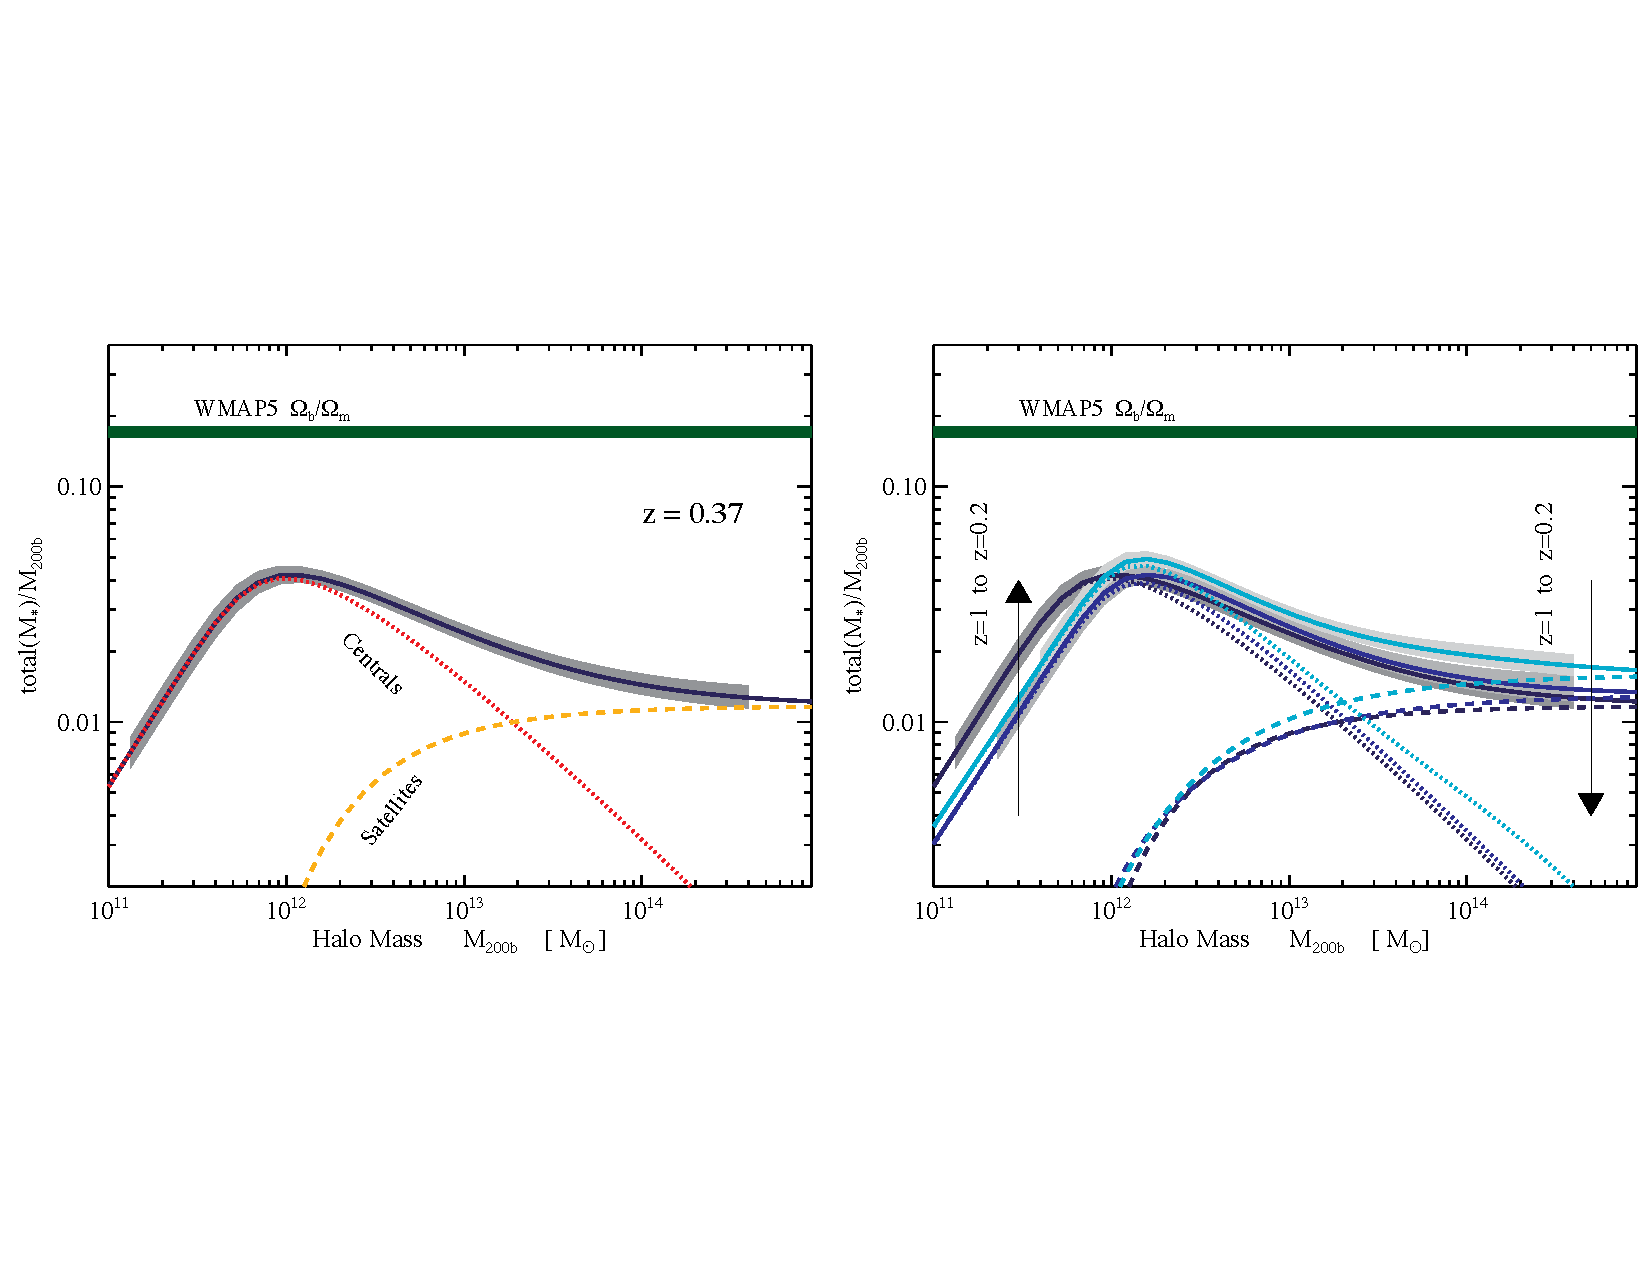
\includegraphics[width=0.9\textwidth]{/Users/apalmese/work/PhD_thesis/thesis_format/chapters/chapter1/figs/total_stellar_content_feb18a.pdf}\caption{Total stellar content locked up in galaxies as a function of halo mass compared to the cosmic baryon fraction measured by the Wilkinson Microwave Probe (WMAP5; Dunkley et al. 2009). Left panel: Our prediction from the z1 bin m ($z < 0.37$). Right panel: Our three redshift bins. z1 is shown by the solid dark blue line, z2 is shown by the blue line, and z3 is shown by the turquoise line. Dotted lines show the contribution to Mtot from the central galaxy and dashed lines show the contribution from satellite galaxies. Shaded regions represent the errors on M tot /M . M tot is dominated by the central galaxy at $M < 2 \times 10^{13} M_\odot$ and by satellites at $M_h > 2 \times 10^{13} M_\odot$.}
%\end{figure}

%\section{Galaxy evolution}
%non-DE
%For a review on galaxies physical properties see \citet{blanton09}
%Halo model\\
%LF/SMF\\


%From \citet{lauthaud}:
%The transition between the two regimes is driven by the steep decline in Mcen/M at $M > 10^{12} M_\odot$ . This decline occurs as the contribution from satellites begins to rise. One might then naturally ask if central galaxies in group-scale halos experience stunted growth simply because stellar mass is accumulating within the halo in the form of satellite galaxies, instead of merging onto the central galaxy. Figure 16 reveals that this is not the case. Indeed, the solid line in this Figure demonstrates that the total stellar mass fraction of halos declines at $M > 10^{12} M_\odot$.


%%%%%%%%%%%%%% GW %%%%%%%%%%%%%%%%

\section{Gravitational waves}\label{sec:introgw}

The first detection of gravitational waves (GW) in 2015 (\citealt{ligogw150914}), which was worthy of a Nobel prize in 2017, and of an electromagnetic (EM) counterpart to a GW event (\citealt{MMApaper}) mark the beginning of a new era of astronomy.

Gravitational waves were predicted by Einstein in 1916 (\citealt{einstein1}; \citealt{einstein2}) within the Theory of General Relativity, and scientists had been searching for them for decades before the first detection. GWs are ripples in the space--time that travel at the speed of light,\footnote{At least within GR predictions. We shall see below that the speed of GWs has been confirmed to be the same as the speed of light, or very close to it.} and are a consequence of Einstein's equations. Suppose that there is a small perturbation $h_{\mu\nu}$ on a nearly flat spacetime, i.e. a Minkowski spacetime with a metric $\eta_{\mu\nu}=diag(-1,1,1,1)$. Then the metric will be:
\begin{equation}
g_{\mu\nu}=\eta_{\mu\nu}+h_{\mu\nu}({\bf x}) \quad {\rm with}\, |h_{\mu\nu}| \ll 1\,.
\end{equation}
In this ``linearised gravity'' regime, in the Lorentz gauge (which is equivalent to a coordinate choice), Einstein's equations simplify to (in vacuum, $T_{\mu\nu}=0$):
\begin{equation}
\Big( -\frac{\partial^2}{\partial t^2}+\nabla^2 \Big) h_{\mu\nu}({\bf x})=0\,,
\end{equation}
which is an ordinary wave equation propagating at the speed of light. Plane waves of the type $h_{\mu\nu}=A_{\mu\nu}{\rm exp} (2\pi i k_\mu x^\mu)$ are a solution, with $k_\mu k^{\mu}=0$. If in addition to the Lorentz gauge, one assumes the so called transverse--traceless gauge (which is also allowed because we have 4 degrees of freedom to specify), and chooses the $z$ axis to be along the direction of wave propagation, the line element can be written with 2 only independent amplitudes, $h_+$ and $h_\times$, 2 independent degrees of freedom for the polarization. It can be shown that the metric perturbation becomes (see e.g. the review by \citealt{riles}):
\[
h_{\mu\nu}({\bf x})=
  \left( \begin{array}{cccc}
   0 & 0 & 0 & 0\\
   0 & h_+ & h_\times & 0\\
   0 & h_\times & -h_+ & 0\\
   0 & 0 & 0 & 0\\
  \end{array}  \right) {\rm exp}[ik(z-t)]\, .
\]

\subsection{Detection}
In order to measure these distortions of spacetime, one needs to define some standard ``ruler'' that is not affected by gravity. The speed of light is a quantity which is not affected by the tidal forces: the idea is to send light to a point where it can be reflected, and measure the return time on a clock at the initial position. Given that we want to measure the proper distance between the initial and reflecting point in order to detect any changes in spacetime, we also need to measure the proper time (i.e. in an inertial frame). The return time of the light beam gives us a measurement of that proper distance. In the simple case in which $A_{xy}=h_\times=0$, the wave propagates with a $+$ polarisation along the $z$ axis, and a photon emitted at time $t$ reaches the position $x=L$ at the time:
\begin{equation}
t_L=t+\int_0^L[1+h_+(t(x))]^{1/2} {\rm d} x \,,
\end{equation}
and in the linearised theory the rate of change of the return time $t_{\rm ret}$ of the photon is:
\begin{equation}
\frac{{\rm d}t_{\rm ret}}{{\rm d}t}=1+\frac{1}{2}[h_+(t+2L)-h_+(t)] \,. \label{eq:tret}
\end{equation}
Note that this change depends on the wave amplitude at the origin when the photon is sent out and when it returns. In the general case, the return time will depend on the amplitude at the reflecting end, too.
The technology used in the gravitational wave detectors such as the Laser Interferometry Gravitational-wave Observatory (LIGO; \citealt{aligo}) and Virgo (\citealt{avirgo}) utilise this concept through laser beams in very large interferometers. They are enhanced (i.e. with an extra mirror) Michelson interferometers. The length of the arms of these detectors is much smaller than the typical wavelength $\lambda$ of a gravitational wave, so that Eq. (\ref{eq:tret}) can be expanded in $L/\lambda$. Unfortunately, the GW amplitudes are too small to produce any change in time detectable with the accuracy of current clocks. However, a measurement of such amplitudes can be made by comparing the variation of the return time in perpendicular directions, as in the arms of interferometers.\footnote{This comparison is allowed by the fact that gravitational radiation is not isotropic.} The length of the arms are typically very large ($L=4$ km for LIGO, 3 km for Virgo) to increase the precision on the actual measured quantity, the \emph{strain} $h=\Delta L/L$, where the change in length $\Delta L$ is due to a gravitational wave and is limited by instrumental and environmental noise. A typical amplitude for a gravitational wave generated by a compact binary system merger at the distance of the Virgo cluster is $h\sim 10^{-21}$. For a detector arm of length 4 km, this corresponds to measuring a change in length of 1/1000 the size of a proton. The strain sensitivity of the detectors depends on the frequency of the wave, and it lies between $10^{-20}-10^{-23}$ for the last LIGO-Virgo observation run over the expected range of compact object binaries frequencies. The strain is comparable to the GW amplitude because a detector with arm length $L$ responds to a GW of amplitude $h$ as $\Delta L \sim hL$. The instruments have recently been upgraded to \emph{advanced} LIGO (aLIGO) and Virgo (AdV or aVirgo), with an increased sensitivity of an order of magnitude, corresponding to an increase in search radius of a factor 10, and therefore of $10^3$ in volume. The previous instrument sensitivity was too low for the rate of observable events to to detect anything with decent probability.

Given that the wavelength of the GW events is much larger than the detectors' length, they can be thought of as antennas that are only able to localise the position of the GW source over broad areas. Triangulating a detection with multiple interferometers can help in constraining the position: a pair of detectors restricts the location to an annulus over the sky, and combining pairs of detectors at different locations allows intersections of these annuli. LIGO interferometers are located in isolated areas by Washington (LIGO Hanford) and Louisiana (LIGO Livingston), and separated by $\sim 3,000$ km, while Virgo is in Pisa (Italy).

Note that the calculations shown in the linearised gravity are only meant for a qualitative understanding, and more sophisticated calculations need to be performed in a practical analysis. For more detailed analyses of gravitational waves, detectors and searches see the reviews by \citet{Sathyaprakash}, \citet{pitkin} and \citet{riles}.

\begin{figure}\centering
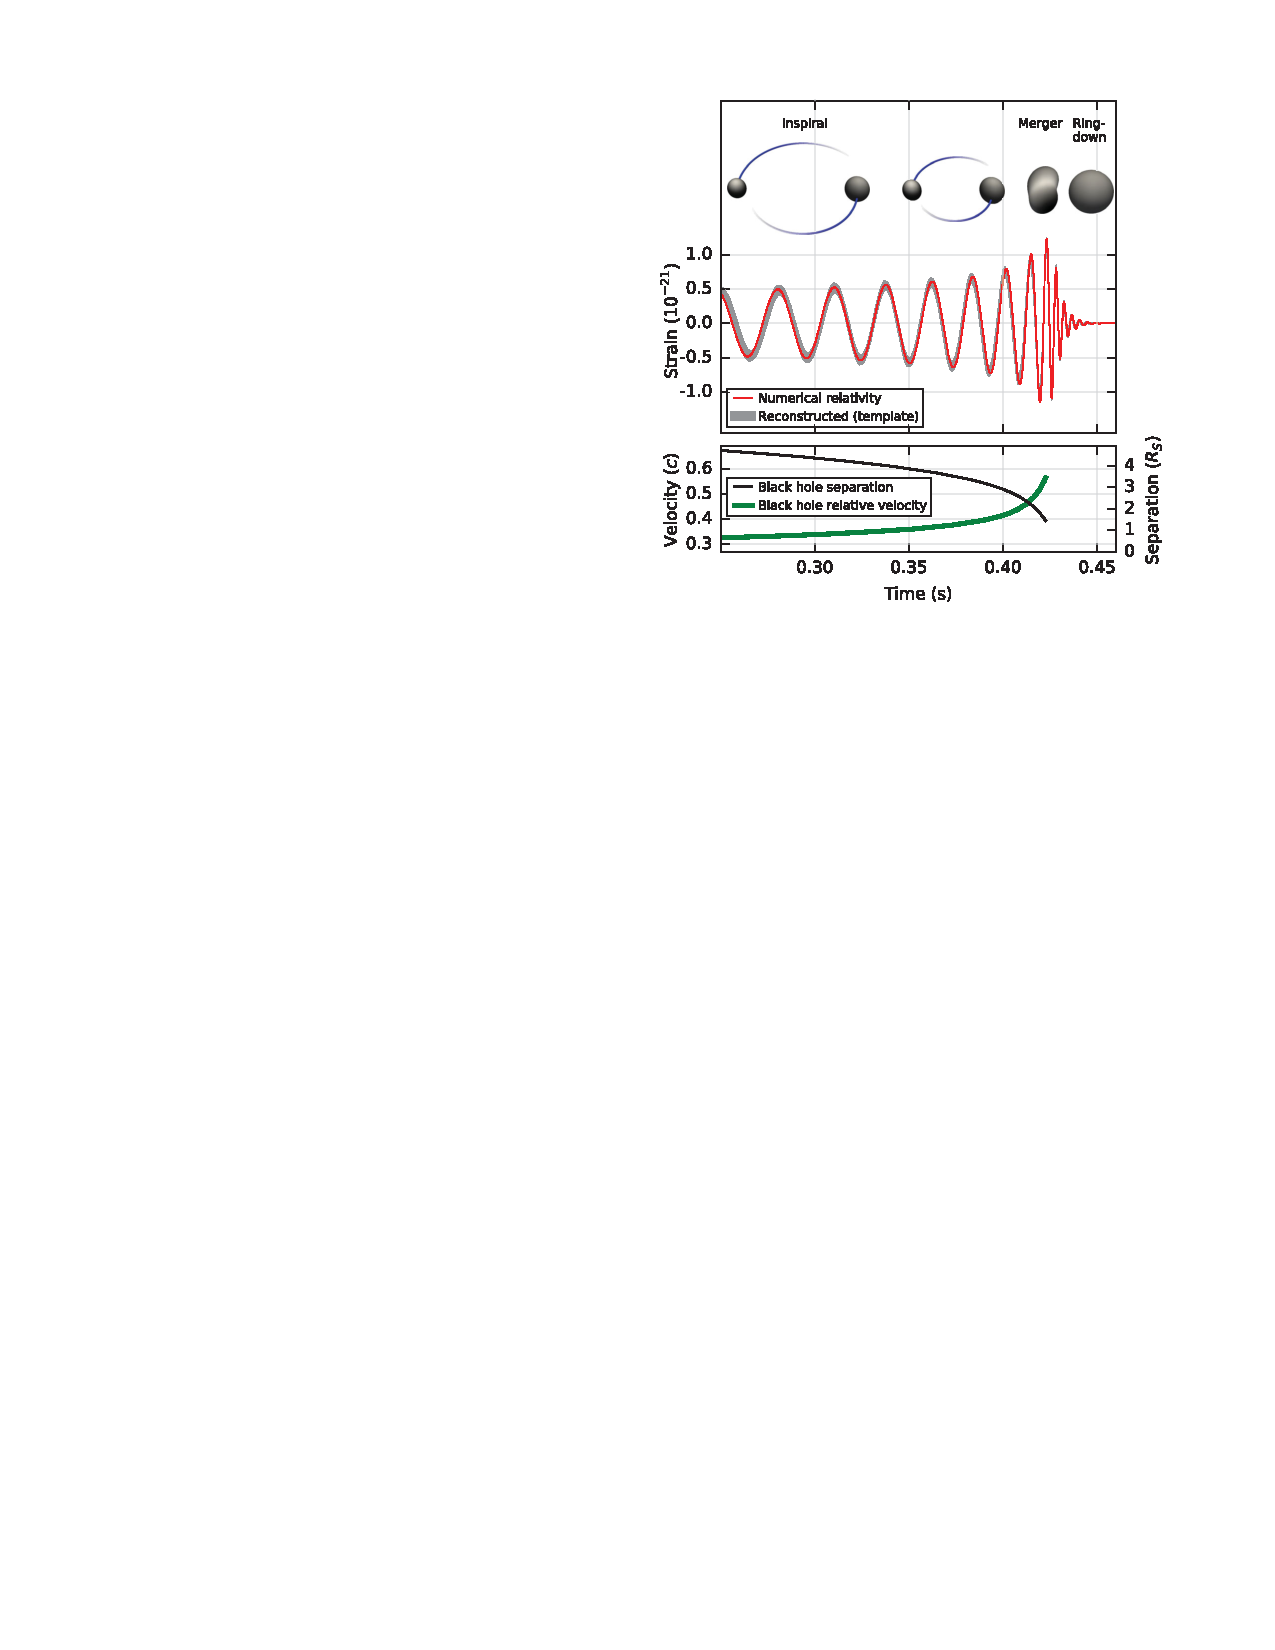
\includegraphics[width=0.7\textwidth]{/Users/apalmese/work/PhD_thesis/thesis_format/chapters/chapter1/figs/GWstrain.pdf}
\caption{Strain amplitude from GW150914, showing the different stages of the binary coalescence and the behaviour with time of the oribital velocity and separation. From \citet{ligogw150914}.}\label{fig:strain}
\end{figure}

\subsection{Sources of GWs}
The most promising sources of gravitational waves detectable by current and upcoming GW experiments are mergers of compact binaries (CB). Considered binaries include binary neutron stars (BNS or NS-NS), binary black holes (BBH or BH-BH) and black hole-neutron star (BH-NS) systems. These systems tend to gradually lose angular momentum while radiating gravitational waves, so that their orbit shrinks as they proceed towards an inevitable collision. The gravitational radiation emitted during the highly relativistic final moments of this process is huge, corresponding to $\sim 5-10\%$ of the initial mass of the system, and this is why we regard CBs as the most promising sources to be detected from Earth. The stages that characterise a CB coalescence can be distinguished into: \emph{inspiral}, \emph{merger} and \emph{ringdown}. During the inspiral phase, one can use a quasi--Newtonian approximation and work out analytic expressions. It can be shown that the GW frequency $f$ and amplitude $h$ for a binary system of objects with masses $M_1$ and $M_2$ in a circular orbit are (\citealt{riles}):
\begin{equation}
f=\frac{1}{8\pi} \Bigg[ \frac{5^3}{G^5 \mathcal{M}^5(\tau-t)^3}\Bigg]^{\frac{1}{8}} \,,
\end{equation}
\begin{equation}
h=\frac{1}{r}\Bigg( \frac{5 G^5 \mathcal{M}^5}{\tau-t} \Bigg)^\frac{1}{4}\,,\label{eq:h}
\end{equation}
where $\mathcal{M}\equiv (M_1M_2)^\frac{3}{5}/(M_1+M_2)^\frac{1}{5}$ is the \emph{chirp mass},  $\tau$ is the time at coalescence and $r$ is the distance to the system. Note that: (i) both frequency and amplitude depend on the chirp mass, so we can estimate its value from a GW measurement, but that at this level one cannot disentangle the values of the two masses; (ii) the frequency diverges as $t\rightarrow \tau$; (iii) the amplitude, effectively our observable, declines as $1/r$, which on cosmological scales has the meaning of luminosity distance. An example of strain signal is shown in Figure \ref{fig:strain}. Other parameters are needed to fully describe the binary system, such as orbit ellipticity, object spin and system orientation.

As the radius of the orbit approaches zero, the post--Newtonian approximation breaks down and numerical simulations are required. The coalescence is expected to form a black hole highly distorted in shape. The remnant is expected to go through a ``ringdown'' phase during which these ``distorsions'' are radiated away through GWs.

Other sources of GW signals include continuous waves from spinning neutron stars and primordial GW background, but these topics go beyond the scope of this thesis.

\subsection{The electromagnetic counterpart}

While no electromagnetic emission is expected from the collision of two black holes due to the lack of baryonic material, the merger of a compact object system containing a NS should produce a range of different transients emitting at different wavelengths, from radio to gamma-ray, and with different timescales (e.g \citealt{bloom09}; \citealt{EMreview}; \citealt{piran}; \citealt{rosswog}). Let us shortly review the processes that lead to such emission, shown in the schematic cartoon in  Figure \ref{fig:cartoon}, as predicted by popular models and simulations.

\begin{figure}\centering
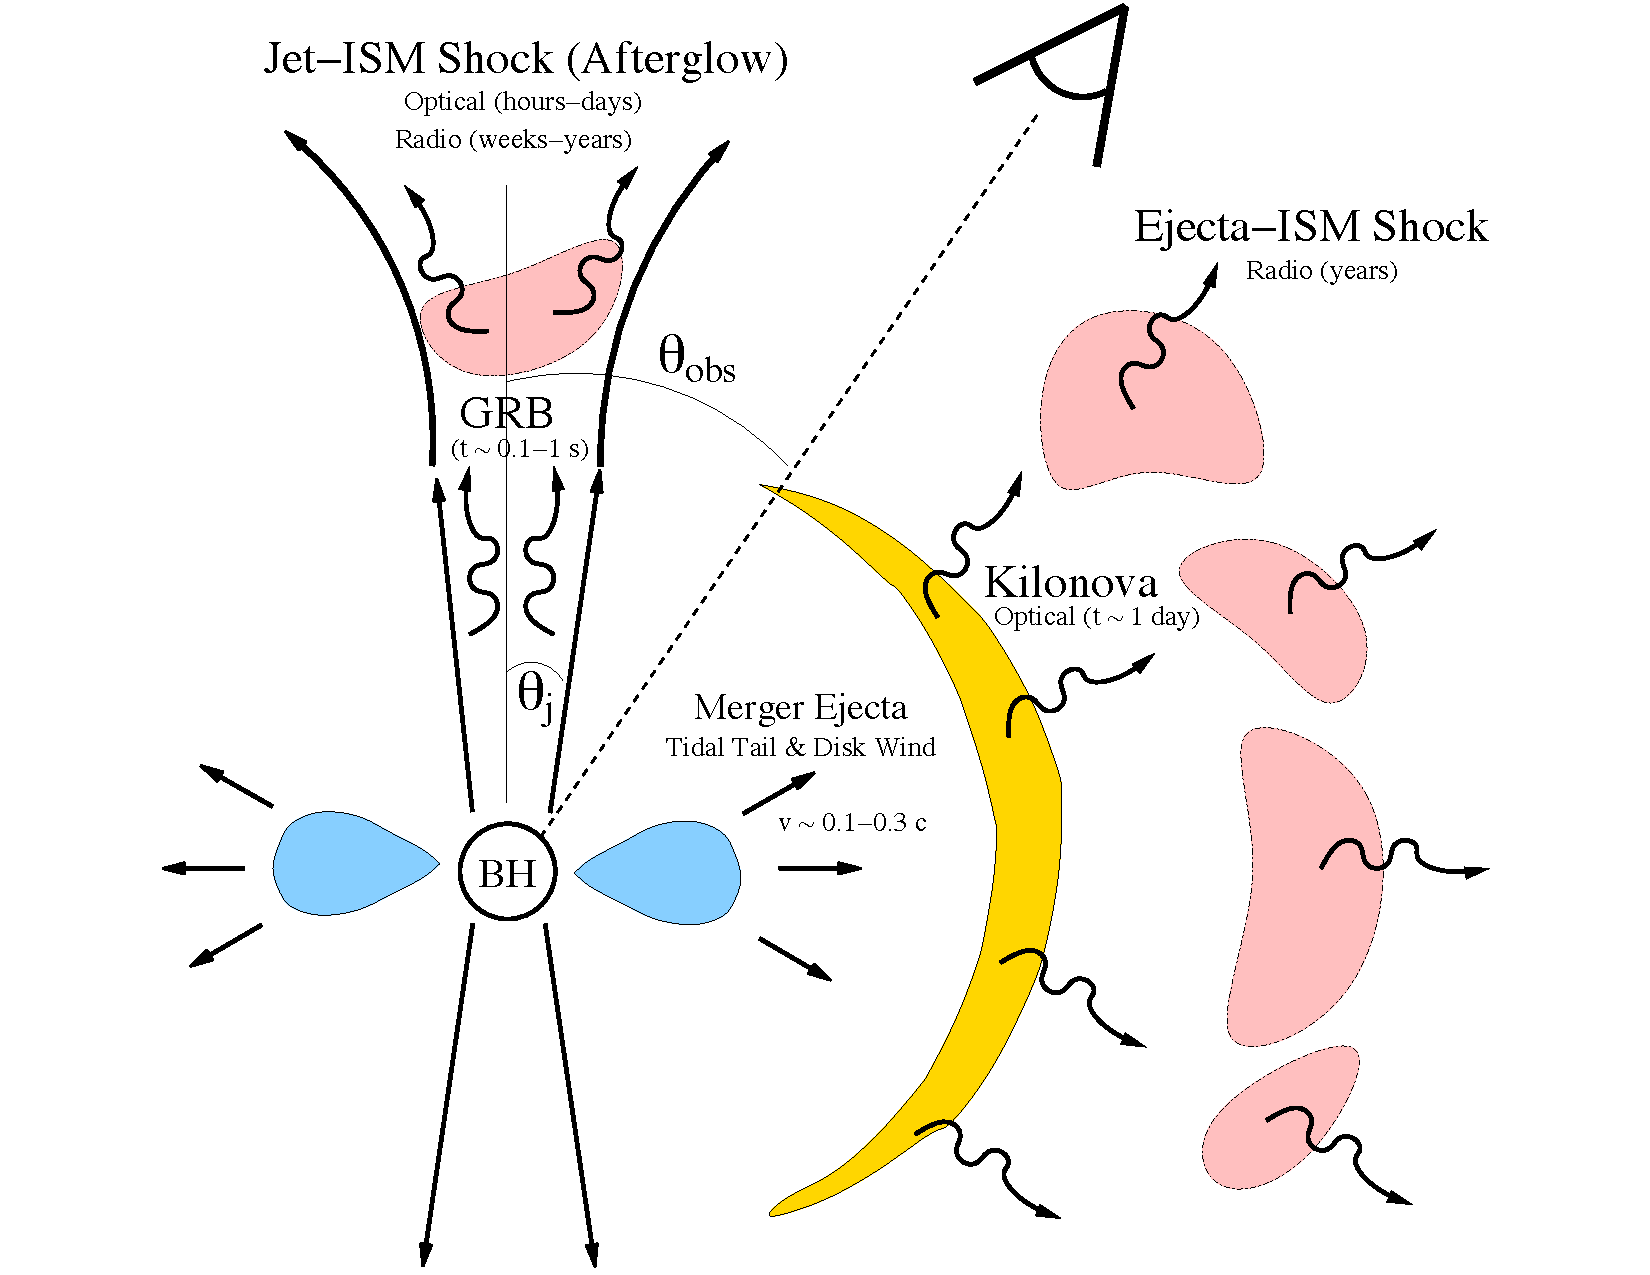
\includegraphics[width=0.6\textwidth]{/Users/apalmese/work/PhD_thesis/thesis_format/chapters/chapter1/figs/cartoon.pdf}
\caption{A schematic cartoon of the origin of the predicted EM counterparts to BNS or NS-BH binaries. From \citet{Metzger}.}\label{fig:cartoon}
\end{figure}

First, depending on the baryonic mass $M_{\rm rem}$ of the binary, the remnant can be a massive, shortly--lived NS, that will eventually collapse into a BH in a matter of milliseconds to seconds. This happens if $M_{\rm rem}\lesssim f M_{\rm max}$, with $f=1.3-1.6$ and $M_{\rm max}$ being the maximum mass of a NS (\citealt{Bauswein}). Otherwise, if the mass of the binary is larger than this limit, the remnant is directly a BH. 

At the time of the merger, part of the binary mass can be ejected in equatorial radial ejecta, part in polar ejecta, where lighter $r$--process\footnote{Rapid--neutron capture processes, or $r$--processes, are a set of nuclear reactions that allows nuclei to capture neutrons more quickly than their radioactive decay. This processes allow the formation of heavy nuclei and occur in regions with high neutron densities (such as NSs).} elements are synthesised. The merger is also expected to produce a centrifugally--supported disk around this remnant. A rapid accretion of the disk is able to power a collimated relativistic jet within seconds from the merger, which can be seen as a sGRB if observed with a viewing angle $\theta_{\rm obs}\lesssim\theta_j$, where $\theta_j$ is the half--opening angle of the jet. 

A non--thermal GRB afterglow, i.e. the emission that follows the GRB at longer wavelengths, is expected to be produced by the interaction of the jets with the surrounding medium. The afterglow is observed in the optical over timescales up to days or weeks by observers at $\theta_{\rm obs}\lesssim2 \theta_j$. An isotropic radio afterglow is expected to be produced when the jet decelerates to moderate relativistic speeds by shocking the inter--stellar matter (ISM).

Slower expanding disk outflows occur on a timescale of $\lesssim$ seconds post--merger, and constitute another site for $r-$process ejecta. Heavier elements, such as gold and uranium, are produced there. The disk ejecta expand quasi--spherically, and radioactive heating is produced by the radioactive decay of the $r-$process nuclei. This powers the isotropic optical-near infrared emission that lasts over timescales of days to 1 week. This emission is what we call a \emph{kilonova},\footnote{Fun fact: the predicted peak luminosities (\citealt{Metzger+10}) of disk ejecta were $\sim1000$ times those from classical novae.}  and it has been identified by \citet{EMreview} as the most promising EM counterpart, given its isotropic nature, as opposed to the collimated GRB. Kilonovae can show a ``blue''  and fast evolving (over timescales of $\lesssim 1$ day, \citealt{Metzger+10}) component in addition to a ``red'' and longer lived one (\citealt{barneskasen,Tanaka}), depending on the electron fraction of the ejecta, and the elements produced. If ejecta contain lanthanides (atomic numbers $57<Z<71$) or actinides ($89<Z<103$), their optical opacity is higher than what it would be with lighter elements, and this delays the observed evolution of the emission which is also shifted towards redder wavelengths.

An analysis of the expected EM counterparts at different wavelengths is described in \citet{EMreview} and \citet{Metzger17} (in the light of GW170817), while a specific review on kilonovae is presented in \citet{Metzger}. These reviews have been mostly followed when writing this introductory section.

There are several motivations to search for the EM counterpart to a GW event:
\begin{itemize}
\item The closest to a cosmologist's heart is surely the possibility of constraining the Hubble constant. Recall from Eq. (\ref{eq:h}) that we can estimate the luminosity distance from the GW amplitude, and if an EM counterpart is detected and associated with an host galaxy having a measured redshift, then $H_0$ can be constrained through Eq. (\ref{boh}). In other words, GW triggers with an identified EM emission can be used as \emph{standard sirens} (\citealt{Schutz86,Holz05}), similarly to what is usually done with Supernovae as standard candles. This analysis has been performed for GW170817 in \citealt{gw170817h0}, and a larger number of GW triggers with an associated EM counterpart will place competitive constraints on $H_0$ (\citealt{Nissanke+10}).
\item To constrain gravity models through estimates of the difference between the speed of light and the speed of gravitational waves (\citealt{Nishizawa16}, \citealt{2017PhRvD..95f3512B} and references therein). In fact, we have seen how GR predicts that GWs propagate at the speed of light. The time elapsed between the detection of the GW signal and the detection of the GRB is at least partially intrinsic to the kilonova model we have described, but it can rule out gravity theories that predict a larger time delay in between the two signal due to their different velocities. This analysis has been performed in \citet{gwspeed}.
\item To study the astrophysics of these systems to constrain the equation of state of NSs and the origin of the $r-$process elements.
\end{itemize}

\subsection{LIGO--Virgo GW triggers}

Coalescences of compact binaries were indeed observed during the first observing runs. 
During the first observing run (O1, September 2015 -- January 2016) only the two LIGO detectors were working, with a sensitivity out to $60-80$ Mpc for BNS. During O1 there were two detections of BBH mergers (GW150914, \citealt{ligogw150914}, and GW151226, \citealt{GW151226}) and a lower significance candidate (LVT151012, \citealt{lvc}).
During O2 (November 2016 -- August 2017) aLIGO was able to detect BNSs out to 100--220 Mpc, and it was joined for the last month by aVirgo, with a horizon reaching 50-60 Mpc (\citealt{ligobns}). Four detections were made during O2: three BBH coalescences (GW170104, \citealt{GW170104}, GW170608, \citealt{GW170608}, and GW170814 \citealt{GW170814}) and a BNS merger (GW170817, \citealt{ligobns}).

\begin{figure}\centering
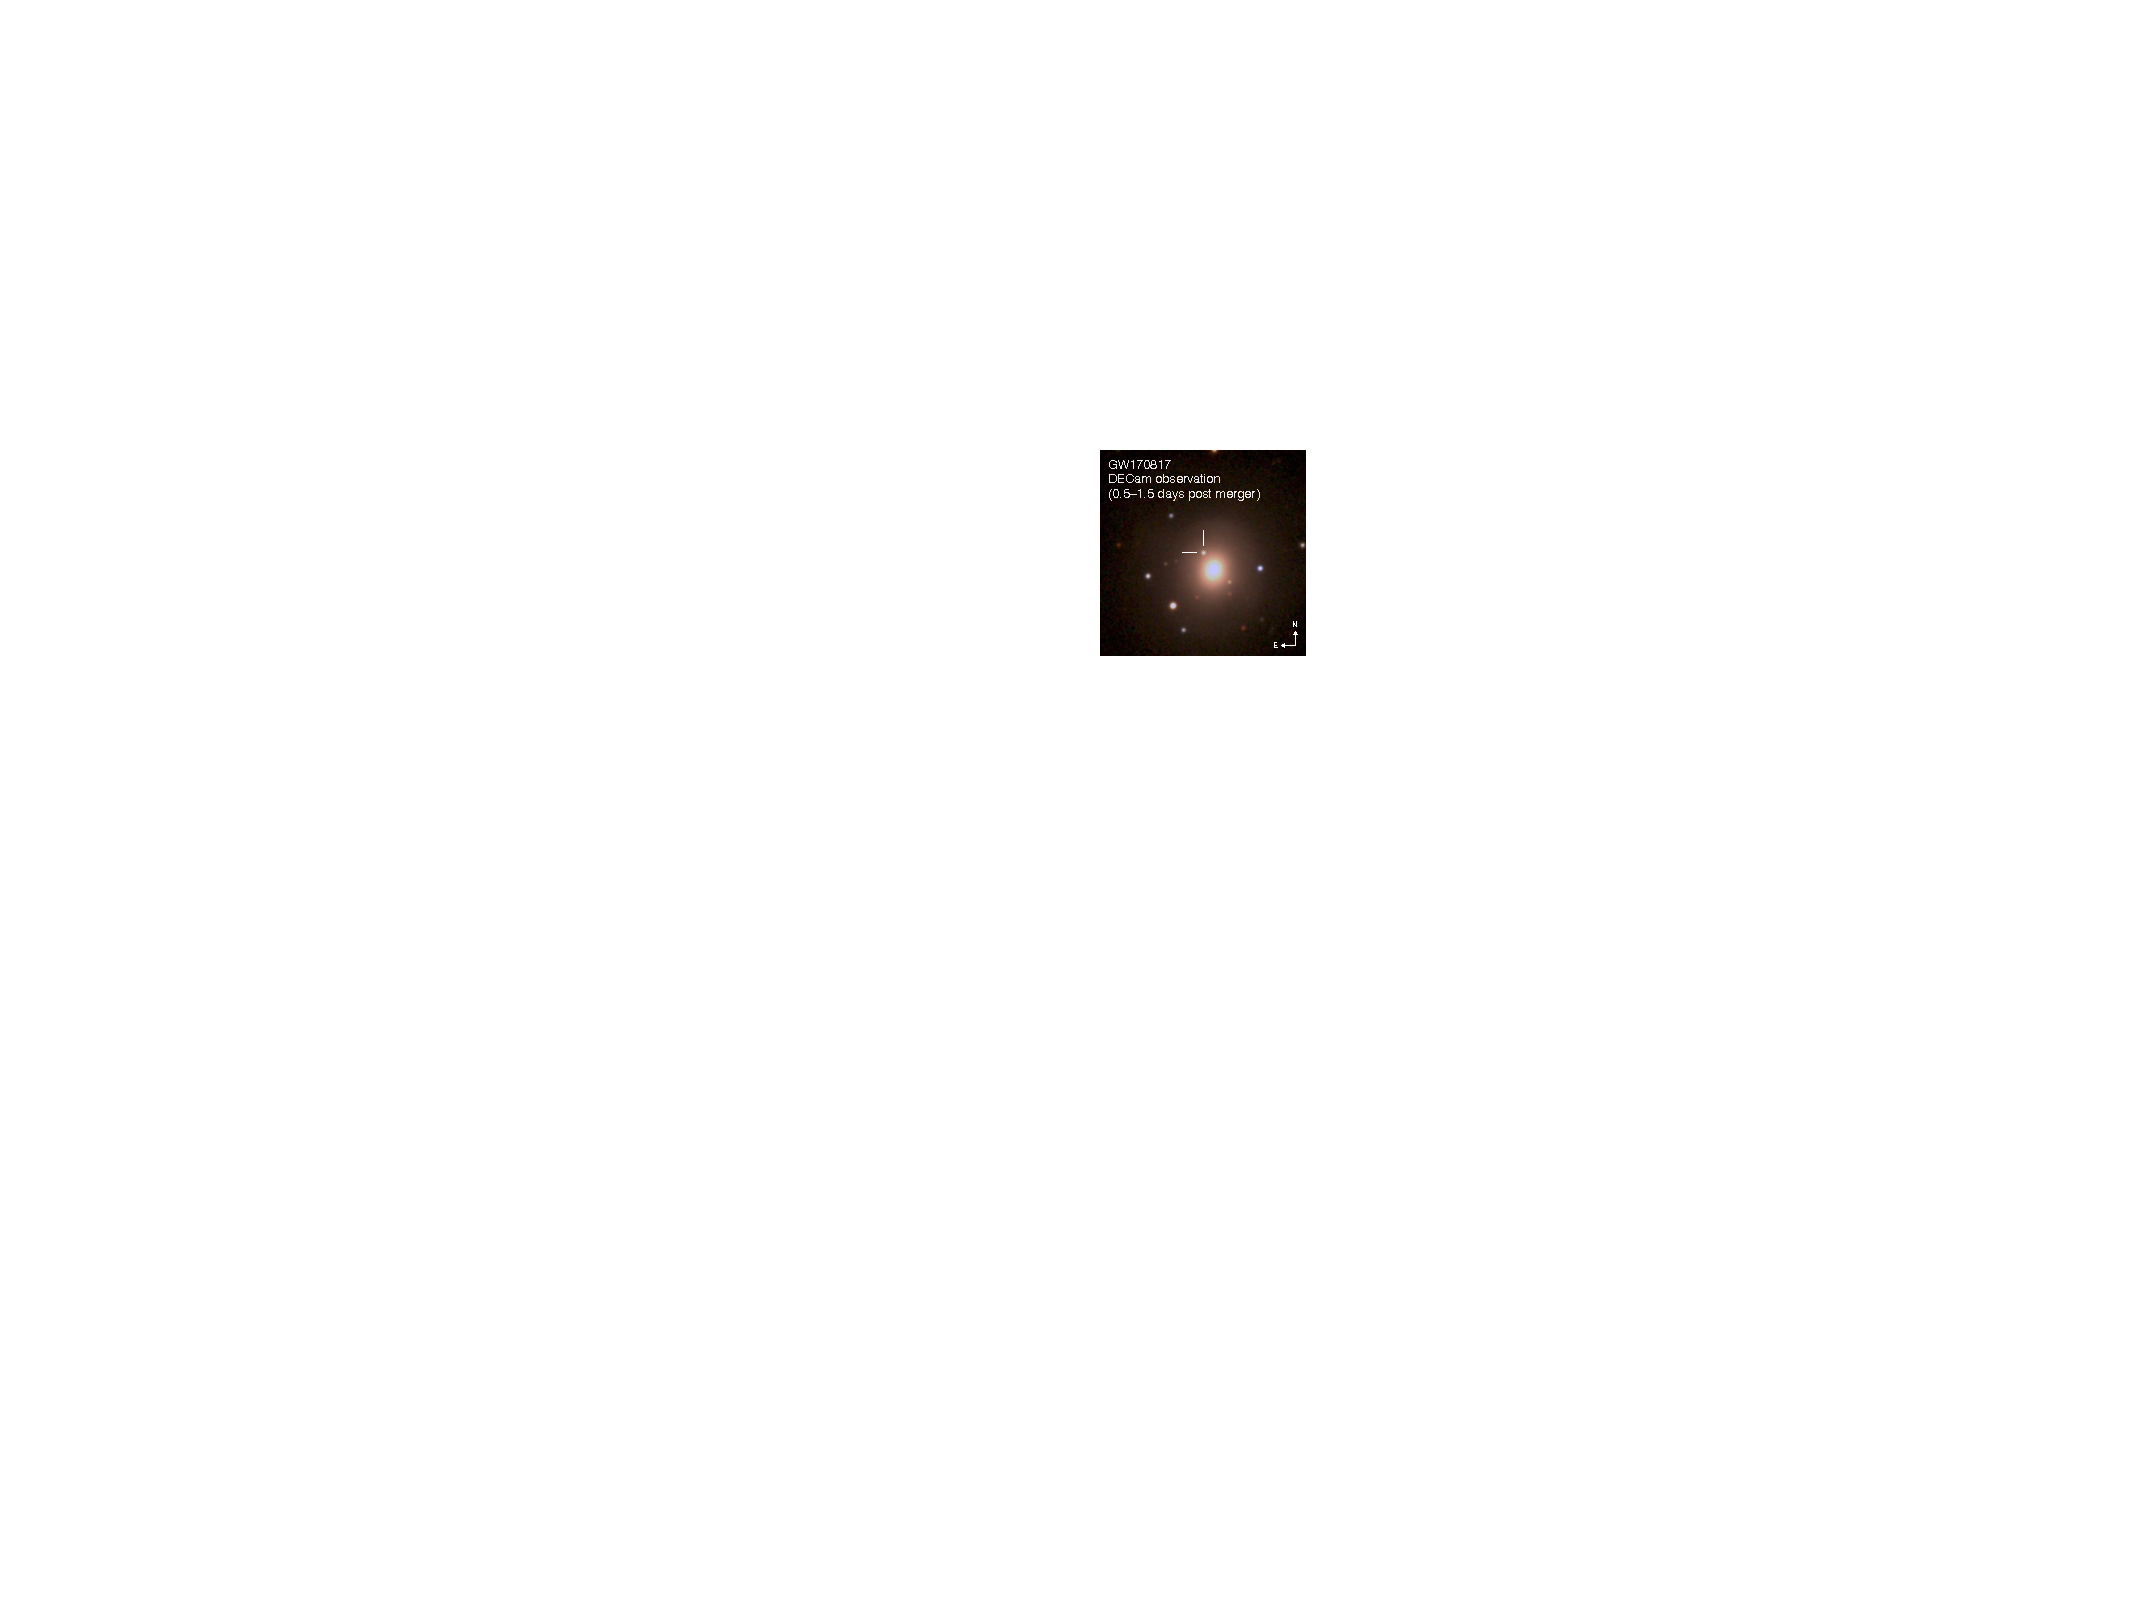
\includegraphics[width=0.5\textwidth]{/Users/apalmese/work/PhD_thesis/thesis_format/chapters/chapter1/figs/GW170817_1d.pdf}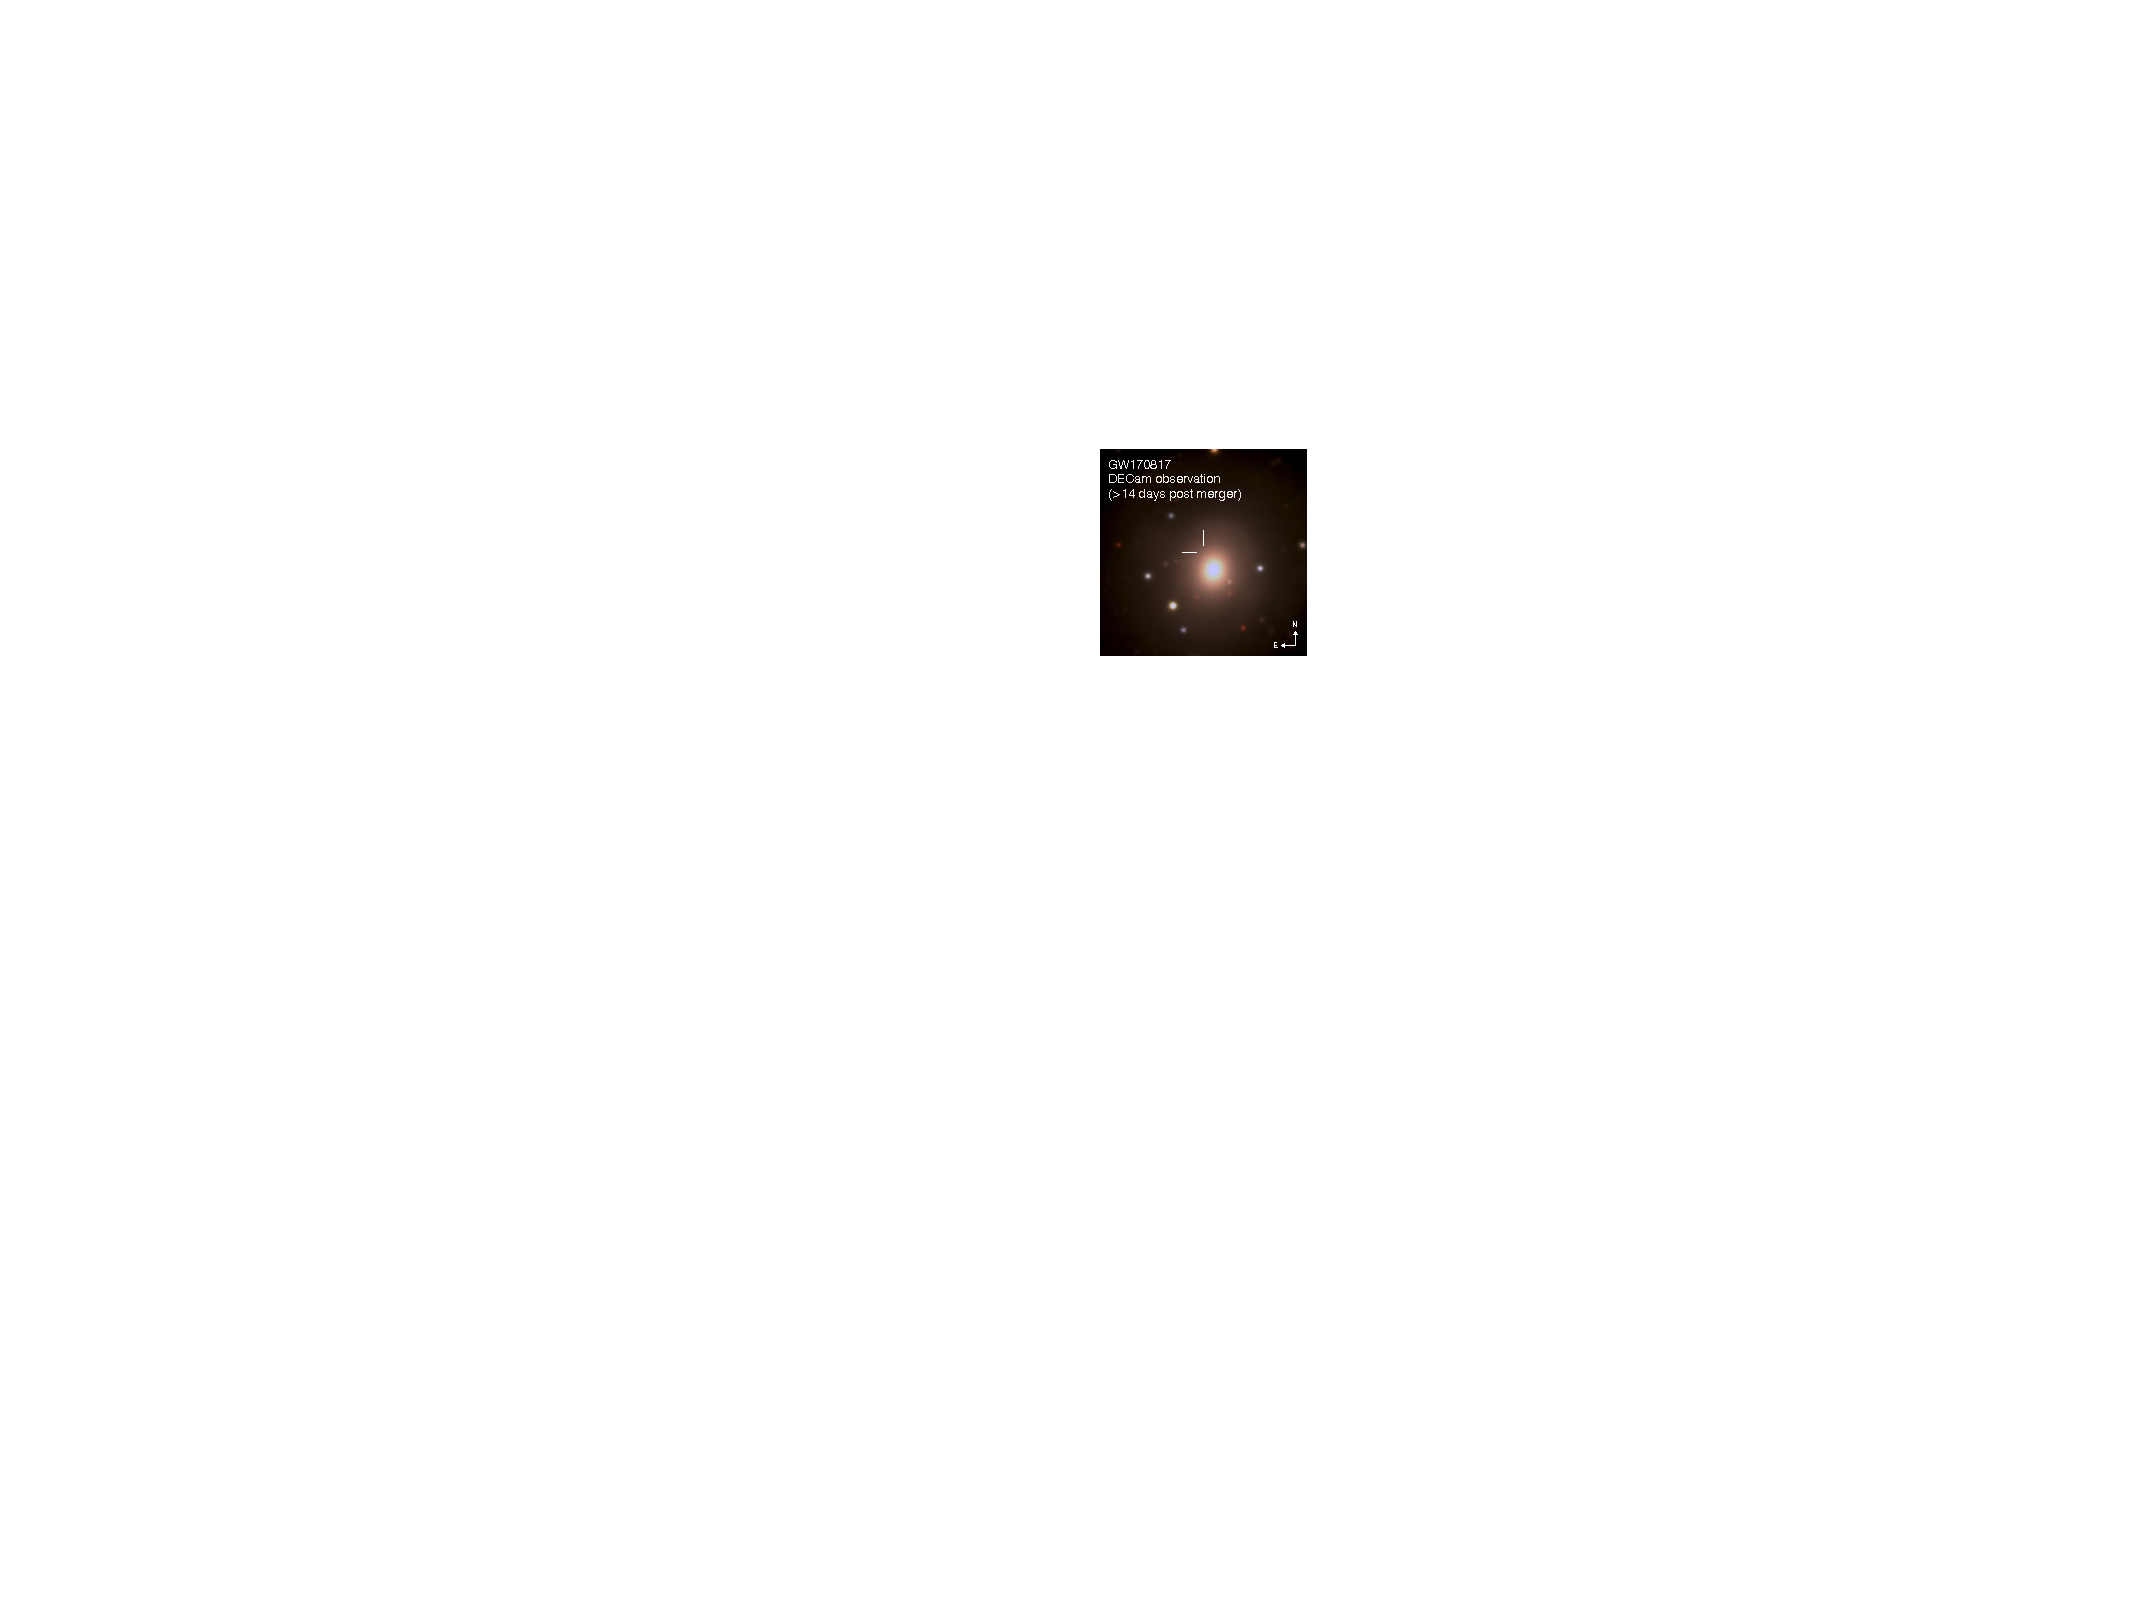
\includegraphics[width=0.5\textwidth]{/Users/apalmese/work/PhD_thesis/thesis_format/chapters/chapter1/figs/GW170817_14d.pdf}
\caption{DECam observations of the kilonova  associated to GW170817. Left panel: coadded image from 0.5--1.5 days post GW trigger. Right panel: coadded image after two weeks from the trigger. The transient has significantly faded away within this timescale, as expected from kilonova models. From \citet{marcelle17}, credits to Will Hartley.}\label{fig:bnsDECam}
\end{figure}

GW170814 was the first detection made by LIGO together with Virgo, and the triangulation of the signal permitted a reduction of the $90\%$ sky localization area from 1160 ${\rm deg}^2$ (with LIGO only) to $60~{\rm deg}^2$. All of the mentioned BBH coalescence detections feature black holes of masses $\sim 20-30~M_\odot$, which are not contemplated by standard stellar evolution theories. It is usually thought that BH of stellar origin can hardly reach these masses due to the large mass loss from stellar winds in the late phases of a massive star life. However stellar evolution models of these late stages are uncertain, and \citet{stellarBH} show that BHs of up to $80~M_\odot$ can have a stellar origin. The study of the origin of these black holes has started to involve more exotic models, including Primordial Black Holes (PBH, e.g. \citealt{pbh}), and it provides the opportunity of constraining the amount of dark matter present in the Universe in the form of PBHs (e.g. \citealt{2017JCAP...09..037R}). Typical luminosity distances of these events are 200--400 Mpc.

GW170817 was the first GW event for which an EM counterpart was confirmed (\citealt{MMApaper}). A description of the EM counterpart to this event with DECam data is presented in Chapter 3. In the meantime, enjoy a DECam coadded image of the first observed kilonova on the left--hand panel of Figure \ref{fig:bnsDECam}.

For a discussion on past and future observing plans with LIGO, see \citet{GWprospects}.

So far, we have discussed how gravitational waves events can have an associated optical counterpart, and how the redshift of the host galaxy is needed in order to make cosmological measurements. We have also discussed how galaxy clusters can constrain cosmology and how they represent an interesting and peculiar environment for galaxy evolution studies. It is now time to introduce the source of data necessary to such analyses: the large galaxy surveys.



%%%%%%%%%%%%% SURVEYS %%%%%%%%%%%%%%%%%%

\section{The era of large galaxy surveys}\label{sec:surveys}

A remarkable number of on--going and planned galaxy surveys will provide data for hundreds of millions, or even billions, of galaxies back to when the Universe was only a fraction of its present age. These surveys were born and funded with the goal of measuring dark energy and other cosmological parameters with unprecedented accuracy.
The constraining power of a particular survey or cosmological probe on DE is often quantified in terms of its \emph{Figure of Merit} (FoM; \citealt{huterer}). The FoM is given by the reciprocal of the area of the $95\%$ confidence limit uncertainty ellipsoid for the DE parameters $w_0,w_a$ defined in Eq. (\ref{wa}). In the Fisher matrix formalism this corresponds to:
\begin{equation}
{\rm FoM} \propto [\sigma(w_0)\sigma(w_a)]^{-1}\, ,
\end{equation}
where $\sigma(w_0)$ $\sigma(w_a)$ are the uncertainties on the parameters.
This choice was first adopted by the Dark Energy Task Force (DETF; \citealt{detf}) as a metric to compare and classify different surveys and methods. 
The DEFT divided dark energy experiments into different Stages. Stage I experiments have provided the data that were known at the time of writing (back in 2009) from observations of Type Ia Supernovae (SN), CMB anisotropies, weak lensing and Baryonic Acoustic Oscillations (BAO). Stage II surveys include DE experiments that were on--going. Stage III comprises on--going medium cost experiments that will improve the FoM by a factor of 3--5 compared to Stage II. Stage IV includes large scale, longer term projects that will improve the FoM by a factor of $\sim 10$ compared to Stage II.

\begin{sidewaystable}
 \centering 
 \begin{tabular}{ccccccc}
  \hline
  \hline
  Project&Dates&Area [deg$^2$]&Data & Spec-$z$ range & Probes &Stage \\
  \hline
BOSS & 2008-2014 &10,000 & Opt-S & $0.3-0.7$ (gals) &BAO & III\\
DES & 2013-2019 &5,000 & Opt-I & -- &BAO, WL & III\\
&&&&&CL, SN &\\ 
eBOSS & 2014-2020 &7,500 & Opt-S & $0.6-2.0$ (gal/QSO) &BAO& III\\
SuMIRe & 2014-2024 &1,500 & Opt-I & -- &WL, CL & III\\
&&& Opt/NIR-S & $0.8-2.4$ (gals) &BAO&\\
HETDEX & 2014-2019 &300 & Opt-S & $1.9-3.5$ (gals) &BAO& III\\
DESI & 2019-2024 &14,000 & Opt-S & $0-1.7$ (gals) &BAO& IV\\
LSST & 2020-2030 &20,000 & Opt-I & -- &BAO, WL& IV\\
&&&&& CL, SN&\\
\emph{Euclid} & 2020-2026 &15,000 & Opt-I & -- &WL, CL& IV\\
&&&NIR-S& $0.7-2.2$ (gals) &BAO&\\
\emph{WFIRST} & 2024-2030 &2,200 & Opt-S & -- &WL, CL, SN& IV\\
&&&NIR-S& $1.0-3.0$ (gals) &BAO&\\

\hline
 \end{tabular}
\caption{A selection of major recent, on--going and future dark energy experiments. Abbreviations in the ``Data'' column refer to optical (Opt) or near-infrared (NIR) imaging (I) or spectroscopy (S). For spectroscopic experiments, the ``Spec-$z$'' column lists the primary redshift range for galaxies (gals), quasars (QSOs). %, or the Lyman-$\alpha$ forest (Ly$\alpha$F). 
Abbreviations in the ``Methods'' column are weak lensing (WL), clusters (CL), supernovae (SN) and baryon acoustic oscillations (BAO). %, and redshift-space distortions (RSD). 
Adapted from \citet{weinbergrev}.}\label{tab:surveys}
\end{sidewaystable}

Table \ref{tab:surveys} presents a representative, albeit not exhaustive, list of on--going and upcoming galaxy surveys, both imaging and spectroscopic. Spectroscopic datasets are usually smaller than photometric ones, due to the time involved in taking spectra, and they usually go down to fainter flux limits than imaging surveys. On the other hand, spectra trace in greater detail the fingerprints of galaxies' stellar populations. As a result, spectroscopic surveys can provide complementary means to constrain galaxy evolution models and cosmology, as well as calibration sets for photometric surveys.

Stage II projects include the famous optical imaging surveys Sloan Digital Sky Survey II (\citealt{sdssII}) and PanSTARRS I (\citealt{panstarss1}), and the \emph{XMM} Cluster Survey (\citealt{romer}) in the X--ray. Stage III imaging experiments comprise DES, described in Section \ref{sec:DES}, and the Hyper--Suprime Camera (HSC; \citealt{hsc}), carrying out similar observations to DES, but to a greater depth on a smaller area. The HSC is only one part of the greater Subaru Measurement of Images and Redshifts (SuMIRe) project. On the spectroscopic side, the Baryon Oscillation Spectroscopic Survey (BOSS; \citealt{boss}) and it successor extended BOSS (eBOSS; \citealt{eboss}) probe the distribution of millions of galaxies and quasars, and the Hobby-Eberly Telescope Dark Energy Experiment (HETDEX; \citealt{hetdex}) maps a smaller area but out to a greater distance. Stage IV projects feature the optical imaging Large Synoptic Survey Telescope (LSST; \citealt{lsst}), the great successor of DES. LSST will image the southern sky every four nights, providing a huge amount of data for transients science (in particular, SN cosmology). The images will be coadded over ten years of observations, resulting in an incredibly deep survey for a ground based experiment.

Space missions include \emph{Euclid} (\citealt{euclid}) and \emph{WFIRST} (Wide Field Infrared Survey Telescope; \citealt{wfirst}), and will provide both imaging and spectroscopic data for billions of galaxies.

Surely datasets mapping huge volumes of the Universe can be exploited for astrophysical studies beyond cosmological parameters. It is in this spirit that gravitational wave follow up programs were born with the goal of observing kilonovae, and that we perform galaxy evolution studies by looking at the astrophysical properties of single galaxies. Surprisingly enough, galaxy surveys have enabled observations of the host galaxy to the first BNS GW signal, so that we could provide a measurement of the cosmological parameter $H_0$. Furthermore, in this thesis we show how galaxy properties can be used to estimate the total mass of galaxy clusters, which again is a necessary step towards cosmological measurements.


\subsection{The Dark Energy Survey}\label{sec:DES}

The DES (for further information see \citealt{descollaboration} and \url{www.darkenergysurvey.org}) is an optical-near-infrared survey that is imaging 5000 ${\rm deg}^2$ of the South Galactic Cap in $grizY$ bands over 525 nights spanning almost six years. The DES filters transmission curves are shown in Figure \ref{fig:filters}. The survey is being carried out using a $\sim3$ $\textrm{deg}^2$ CCD
camera (the DECam, see \citealt{flaugher}) mounted on the Blanco 4-m telescope at the Cerro Tololo Inter-American Observatory (CTIO) in Chile. DES started in 2012 with a testing period (November 2012 -- February 2013) called Science Verification (SV)\footnote{For public data release see: \url{http://des.ncsa.illinois.edu/releases/sva1}}. The data used in this thesis come from SV and from the first three years (Y3) of observations (September 2013 -- February 2016), which cover $\sim5,000~ {\rm deg}^2$ with up to 4 passes per filter. The DES Y3 footprint, which corresponds to the final footprint, is shown in black in Figure \ref{fig:footprint}. Some of the data used (the wide-field coadd source catalogs) is now publicly available at \url{https://des.ncsa.illinois.edu/releases/dr1} and described in \citet{dr1}. Target of opportunity data from the fourth year of observations are also used in the GW follow up work. At the time of writing, five observing seasons have been completed.

\begin{figure}\centering
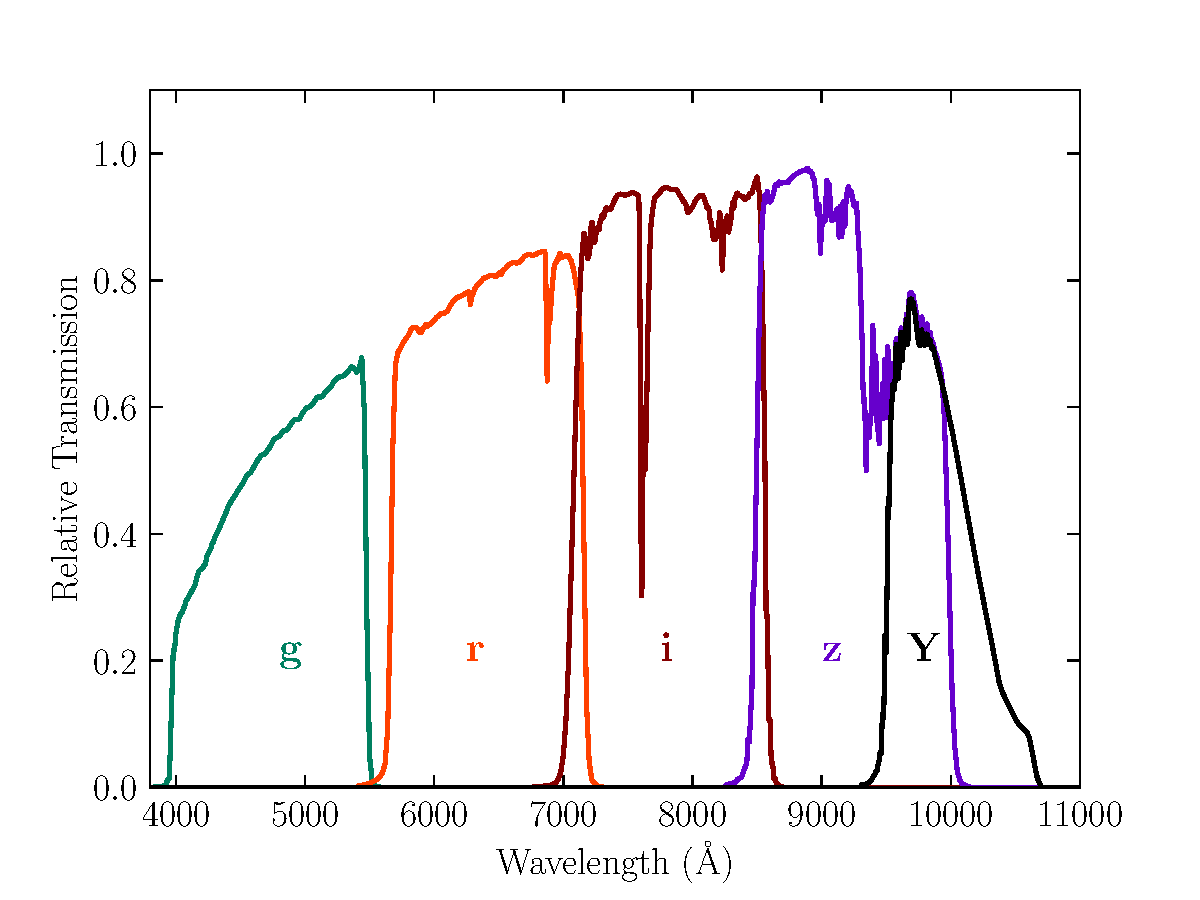
\includegraphics[width=0.6\textwidth]{/Users/apalmese/work/PhD_thesis/thesis_format/chapters/chapter1/figs/dr1_bandpass.pdf}
\caption{DES filters transmission curves. From \citet{dr1}.}\label{fig:filters}
\end{figure}
\begin{figure}\centering
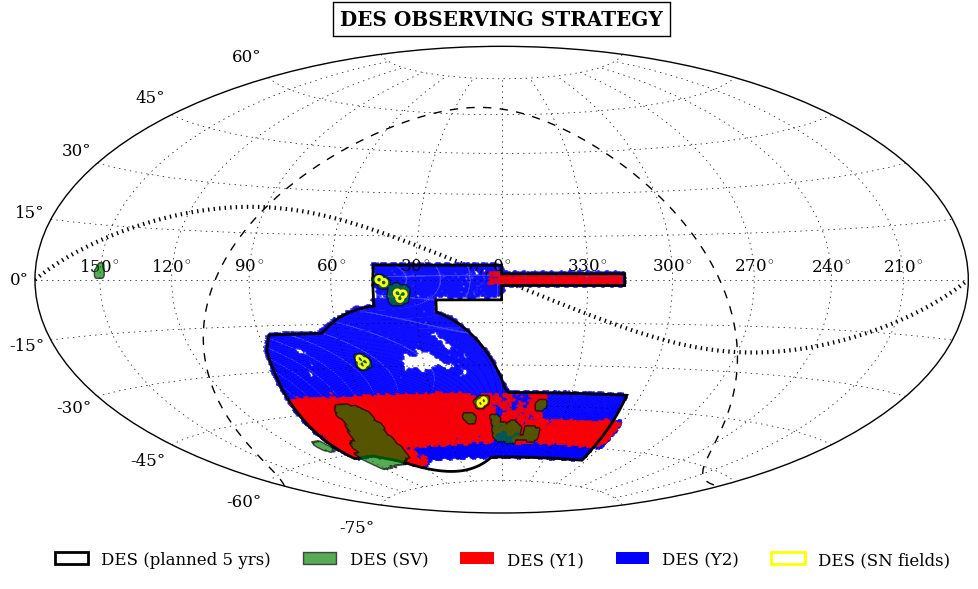
\includegraphics[width=0.8\textwidth]{/Users/apalmese/work/PhD_thesis/thesis_format/chapters/chapter1/figs/footprint_Y1.png}
\caption{DES footprint. The green area is covered by the Science Verification data, used in Chapter 2 and 4. The red area represents the observations from the first year of observations, and it is the area studied with the Y1 redMaPPer clusters in this thesis (Chapter 6). The 5 years planned footprint is shown by the black contours, and it is the same area covered by the Y3 data used in Chapters 3, 5 and 6. The difference between Y3 and Y5 is in the number of passes, and therefore the depth. Plot from \citet{nonDE}.}\label{fig:footprint}
\end{figure}

The survey strategy is designed to optimize the photometric calibration by tiling each region of the survey with several overlapping pointings in each band. This provides uniformity of coverage and control of systematic photometric errors. This strategy will allow DES to determine photometric redshifts of $\sim 300$ million galaxies to an accuracy of $\sigma(z) \simeq 0.07 $ out to $z \gtrsim 1$, with some dependence on redshift and galaxy type, and cluster photometric redshifts to $\sigma(z) \sim 0.02$ or better out to $z \simeq 1.3$ (\citealt{descollaboration}). It will find $\sim 380,000$ groups and clusters and also provide shapes for approximately 200 million galaxies for weak lensing studies. The final depth of the survey will be similar to that of the SV data, where the median $10\sigma$ depths are $g\sim24.45, r\sim24.30,i\sim23.50,z\sim22.90, Y\sim21.70$. The Supernova fields (shown in yellow in Figure \ref{fig:footprint}) are observed to a greater depth.

The DES Data Management (DESDM) pipeline was used for data reduction, as described in detail in \citet{sevilla}, \citet{desai} and \citet{dataproc}. The process includes calibration of the single-epoch images, which are co--added after background subtraction and then cut into tiles. The source catalogue was created using \textsc{Source Extractor (SExtractor}, \citealt{sextractor}) to detect objects on the $riz$ co-added images. 

The data from DES will allow high precision measurements of dark energy and dark matter through the four cosmological probes previously described: weak gravitational lensing, galaxy clusters abundance, galaxy angular clustering and Supernovae. Several papers using these methods have recently been published for the early DES data covering the Y1 area, in particular from weak lensing and galaxy clustering (\citealt{Y1key}; \citealt{gruencosmo}; \citealt{DESBAO}; \citealt{DESH0}). The DES collaboration has also been able to publish significant work beyond cosmology and Dark Energy, including Milky Way studies, Trans-Neptunian Objects and much of the work included in this thesis regarding galaxy evolution and gravitational waves. See \citet{nonDE} for an overview on non-Dark Energy studies with DES.\\

The data used in this thesis also includes Anglo-Australian Telescope (AAT) target of opportunity time data. Other publicly available datasets have been used (VHS, HST, 2dF, 6dF, 2MASS).

\section{Thesis Outline and notation}

This thesis is structured as follows:

\begin{itemize}
\item In {\bf Chapter 2} I describe the methods used to derive galaxy properties (mainly stellar mass) and redshifts from galaxies' Spectral Energy Distribution. I introduce a method that uses a Bayesian Model Averaging technique, and show how I have produced photo-$z$ estimates for early DES data. An approach to compute stellar masses with machine learning techniques is also introduced.
\item In {\bf Chapter 3} I show how large galaxy samples with available redshifts and properties are fundamental for electromagnetic follow ups of gravitational wave events. Furthermore, they can be used to understand the formation and evolution of the binary systems they contain. An analysis of this type is presented for the golden event GW170817.
\item {\bf Chapter 4} includes a study on early DES data showing that stellar masses can be estimated in a robust manner with DES, in particular concerning galaxy clusters. A first estimate of stellar mass fraction in clusters from DES is presented.
\item In {\bf Chapter 5} I introduce a promising cluster mass proxy, $\mu_\star$, based on stellar masses. Its performance is calibrated against X-ray and weak lensing measurements.
\item {\bf Chapter 6} shows cluster evolution results for $\sim 80,000$ DES clusters. We measure the stellar--to--halo mass relation and the stellar mass function for central galaxies and satellites. Other results on central galaxies and ICL are shown.
\item Finally, {\bf Chapter 7} is dedicated to the conclusions of this work and to future prospects for expanding my GW host analyses to binary black hole events and to BNS triggers from the fast approaching third LIGO observing season. The plan for producing $\mu_\star$ for Voronoi--Tesselation clusters over the DES Year 3 area is also already undergoing.

\end{itemize}
Throughout this work we assume a $\Lambda$CDM flat cosmology with $h=0.7$, $\Omega_m = 0.3$, $\Omega_\Lambda =0.7$ unless otherwise stated. The notation adopted for the cluster mass and radius follows the one often used in literature. The radii of spheres around the cluster centre are written as $r_{\Delta m}$ and $r_{\Delta c}$ where $\Delta$ is the overdensity of the sphere with respect to the mean matter density (subscript $m$) or the critical density (subscript $c$) at the cluster redshift. Masses inside those spheres are therefore $M_{\Delta m}=\Delta \frac{4 \pi }{3}r^3_{\Delta m}\rho_m$ and similarly for $M_{\Delta c}$.  In the following, we quote $\Delta=200$, which roughly corresponds to the density contrast at virialisation for a dark matter halo at $z=0$. In order to convert between the different mass definitions we use the Python Colossus tools (\citealt{colossus}). Logarithms indicated as Log have base 10. Errors quoted are $1\sigma$, unless otherwise stated.







\clearemptydoublepage
\chapter{Galaxy SED fitting methods and applications}\label{chp:sed}

\begin{flushright}
  {\em ``Everything we see hides another thing, we always want to see\\ what is hidden by what we see.''}\\

\ \

\normalsize
{Ren\'e Magritte}  
\end{flushright}


\noindent{\emph{The work presented in this Chapter contains part of {\bf Palmese et al., 2018}, currently in the DES review process, and of my contribution to the SV public release and DES SV papers with photometric redshift estimation with ANNz2. The machine learning method for stellar mass estimation is unpublished.}}\\


Fundamental properties of the unresolved stellar populations within galaxies are encoded in the galaxy Spectral Energy Distribution (SED) that we observe. These include the Star Formation History (SFH), stellar mass, initial mass function (IMF) and the metallicity. This information are further folded in with the redshift of galaxies. Extracting as much information as possible from the DES galaxy SEDs is the first goal of this thesis, as the derived properties are fundamental to the analyses that we want to make for gravitational wave source host galaxies and clusters. Thankfully, a huge effort has been spent by the astrophysical community to model and fit SEDs of unresolved stellar populations over the past decades.
In this Chapter we first provide an introduction to redshift estimation and stellar population synthesis models, then we describe the methods used in this thesis to evaluate galaxy properties, from photometric redshifts to stellar masses and star formation rates. In particular, we present a code written by James Annis and myself that uses Bayesian Model Averaging to evaluate galaxy properties that we have made publicly available. We show the first application of machine learning methods to stellar mass estimates from photometric data. Finally, we present some applications of these methods with DES data.

\section{Redshifts}
We recall that the redshift of a galaxy is defined in Eq. (\ref{eq:z}) as:
\begin{equation}
z\equiv \frac{\lambda_{\rm oss}}{\lambda_{\rm em}}-1\, ,
\end{equation}
though not all of it is due to the expansion of the Universe as in Eq. (\ref{eq:z}). The redshift of a galaxy includes contributions coming from the cosmological redshift due to the expansion of the Universe ($z_H$), from peculiar motions with respect to the observer ($z_{\rm phys}$) and possibly to gravitational redshifts ($z_{\rm grav}$, due to galaxies motion within gravitational potential wells), so that:
\begin{equation}
z_{\rm tot} = z_H+z_{\rm phys}+z_{\rm grav}\,.
\end{equation}
The gravitational redshift is usually neglected as it is a very small contribution to the total redshift.\footnote{Works on gravitational redshifts in clusters and galaxies have tried to estimate this contribution through statistical methods such as stacking (e.g. \citealt{wojtak}; \citealt{sadeh15}).}. Peculiar motions can arise from the motion of Earth around the Sun (with a velocity of $\sim 29~{\rm km~s^{-1}}$), the Milky Way's motion with respect to the CMB reference frame ($\sim 630 ~{\rm km~s^{-1}}$ corresponding to $z \sim 0.002$) and orbital motions of galaxies around each other or in cluster potential wells. The galaxies' velocity dispersion in clusters can reach values of $\sim 1500 ~{\rm km~s^{-1}}$ (corresponding to $z\sim 0.005$).

Photometric surveys such as DES measure the redshift of galaxies through photometry, and the estimated redshifts are called photometric redshifts or photo-$z$'s. Photo-$z$'s have been introduced back in the 60s by \citet{baum}, and they have been extensively studied and utilised since the advent of the recent wide-field photometric surveys. While spectroscopy can produce more precise redshift measurements, it is technically arduous work to measure spectra for hundreds of millions of galaxies in a reasonable time span using current technology. While a whole region of galaxies can be imaged with DECam at once, spectroscopy can only be obtained for those galaxies that can be targeted with slits or fibers. Even though photo-$z$'s are subject to large uncertainties, some analyses, such as weak lensing, can benefit more from larger number statistics than from precise redshift measurements. The requirements on the photo-$z$ accuracy for a galaxy survey are usually computed from the requirements on the estimates of cosmological parameters. The requirements on DES redshifts are defined through several metrics computed for a sample of galaxies that has both a photo-$z$ estimate and a reference redshift given by spectroscopy. We assume that those spectroscopic redshifts are the true redshifts of galaxies. The metrics are defined in \citet{sanchez}:
\begin{itemize}
\item $\overline{\Delta z}$: the mean of the bias distribution $\Delta z$, given by the difference between estimated photo-$z$'s and the reference redshifts.
\item $\sigma_{\Delta z}$: the standard deviation of the bias distribution.
\item $\sigma_{68}$: the scatter expressed as the half--width of the bias distribution around the median of the $\Delta z$ distribution, containing $68\%$ of the galaxies. This scatter is required to be $<0.12$ for DES.
\item ${\rm out}_{2\sigma}$: the outlier fraction, i.e. the fraction of galaxies with $|\Delta z - \overline{\Delta z}|>2\sigma_{\Delta z}$, which is required to be $<0.1$.
\item ${\rm out}_{3\sigma}$: the fraction of galaxies with $|\Delta z - \overline{\Delta z}|>3\sigma_{\Delta z}$, which is required to be $<0.015$.
\end{itemize}

\begin{figure}\centering
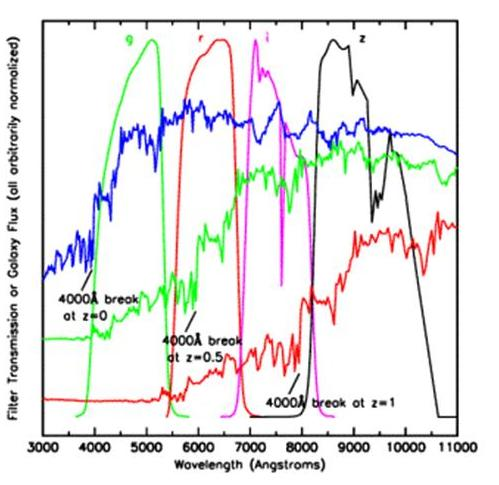
\includegraphics[width=0.5\textwidth]{/Users/apalmese/work/PhD_thesis/thesis_format/chapters/chapter2/figs/filters.jpg}\caption{DECam $griz$ filters with a galaxy spectrum redshifted from $z=0$ to $z=1$. The 4000 \AA~ break can be measured with DECam filters over this redshift range. From the DES Figures library.}\label{fig:filtersz}
\end{figure}

One of the main features of galaxies' SEDs that allow us to measure redshifts with DES is the relatively sharp drop at 4000 \AA: the 4000 \AA~ break. This feature is produced by the absorption of various metallic lines around similar wavelengths, and can be further enhanced by a deficiency of young, blue stars (e.g. \citealt{1985ApJ...297..371H}). The drop is shown in the blue line in Figure \ref{filters}, which represents the spectrum of a typical galaxy at $z=0$. For more distant galaxies the 4000 \AA~ break is shifted towards longer wavelengths, as shown in green and red lines in the plot. This feature is covered by the DES filters out to redshifts just above $z\sim 1$, hence we do not (usually) exceed this redshift with DES analyses.

For DES galaxy evolution and clusters studies, objects are usually at cosmological distances (mostly $0.1<z<1$) so the only contribution to the redshift we consider from photometric data is due to the Hubble expansion. The remaining parts are negligible compared to $z_H$ and well below our photometric redshift uncertainty. GW follow up studies are an exception, as GW sources are in the local universe (usually $z<0.1$) and the redshift estimation becomes tricky with DES data alone, and we require spectroscopic data. The Supernova rejection study is exempted from a spectroscopic follow up as it falls again into the cosmological distance regime.

Note that in some analysis, estimation of the full redshift probability density function (PDF) may be useful (or from it, even just a random draw). Some redshift estimation codes are able to provide that as their output, although storing and sharing a full PDF for each entry in a large galaxy sample such as DES is a known issue (see e.g. \citealt{rau}).

\section{Stellar population synthesis modeling}\label{sec:SPS}
The spectral evolution of galaxies is usually studied through what we call ``Stellar Population Synthesis'' (SPS) modeling, or ``evolutionary synthesis'' modeling. This method relies on stellar evolution models to constrain stellar populations with a certain metallicity and age; the first synthesis models of this type were developed in the late 60s and 70s (e.g. \citealt{tinsley}; \citealt{tinsley72}; \citealt{searle}).  Note that in the following we describe a commonly used, though not universal, methodology. 

\begin{figure}\centering
\includegraphics[width=0.7\textwidth]{/Users/apalmese/work/PhD_thesis/thesis_format/chapters/chapter2/figs/f1.pdf}\caption{Schematic illustration of stellar population synthesis modeling, from \citet{conroy}.}\label{fig:csp}
\end{figure}

\subsection{Simple stellar populations}
The first step in constructing SPS models is building the simple stellar population (SSP) models, i.e. the evolution over time of a stellar population having a single metallicity and age. The time $t$ and metallicity\footnote{The mass fraction in elements heavier than helium} $Z$ dependent SED of an SSP $f_{\rm SSP}$ is given by (\citealt{conroy}):

\begin{equation}
f_{\rm SSP} (t,Z) = \int^{m_{\rm up}}_{m_{\rm lo}} f_{\rm star}[T_{\rm eff} (M_\star), {\rm Log} ~g(M_\star)|t,Z] \phi(M_\star) {\rm d} M_\star\, , \label{eq:ssp}
\end{equation}
where $M_\star$ is the stellar mass at the zero--age main sequence.
The constituents of Eq. (\ref{eq:ssp}) are:
\begin{itemize}
\item Isochrones from a stellar evolution theory. Isochrones represent the position of stars in the Hertzsprung--Russell diagram with same age and metallicity. The theory has lower and upper limits ($m_{\rm lo}$ and $m_{\rm up}$) on stellar masses and the isochrones dictate the relation between the effective temperature $T_{\rm eff}$, the surface gravity $g$ and $M_\star$ at each time and metallicity values. Some popular isochrones include the Padova (\citealt{bertelli}; \citealt{girardi}) and the BaSTI (\citealt{pietrinferni}) models.
\item Stellar spectra $f_{\rm star}$. These are derived from stellar spectral libraries, that deal with converting the stellar evolution outputs into actual spectral energy distributions. Usually several libraries are used together in order to come a wider range of the parameter space. Libraries can be theoretical (e.g. BaSeL, \citealt{basel1}, \citealt{basel2}, \citealt{basel3} which is the most used theoretical stellar library) or empirical (e.g. STELIB, \citealt{stelib}, MILES, \citealt{miles}).
\item The Initial Mass Function $\phi(M_\star)$, which gives the stellar mass distribution of the zero--age main sequence. Typically, this has the form of a power law or a broken power law. A set of widely used IMFs is discussed in Chapter 6.
\end{itemize}
The choice of the IMF is an important step as the IMF not only determines the normalization of the $M_\star/L$, but it also significantly impacts composite stellar populations SEDs. In fact, the luminosity of an SSP is dominated by the stars at the turnoff mass, which translates into a range of several turnoff masses within a composite population. The most widely used IMFs differ at the low mass end ($M_\star <1 M_\odot$): stars in this regime dominate the stellar mass of a galaxy but contribute very little (a few percent) to the overall galaxy bolometric luminosity for an old stellar population. It is thus impracticable to discern between these different models with the photometric data from DES without introducing degeneracies with stellar mass/mass-to-light ratio.

\subsection{Composite stellar populations}

A galaxy's spectrum can be built up by adding the spectra of several SSPs of different ages and metallicities into a Composite Stellar Population (CSP) model of the form:

\begin{equation}
f_{\rm CSP} (t) = \int^{t'=t}_{t'=0} \int^{Z_{\rm max}}_{Z=0} \big(  f_{\rm SSP}(t',Z)  SFR(t-t')P(Z,t-t')e^{-\tau_d(t')}+Af_{\rm dust}(t',Z) \big){\rm d} t' {\rm d} Z\, ,\label{eq:csp}
\end{equation}
The ingredients needed to build such SED are:
\begin{itemize}
\item The star formation history (SFH), dictating the ages of stars from SSPs. This is given in the form of a star formation rate (SFR) as a function of time. Widely adopted SFHs include very simplystic models, such the exponential or $\tau$ model (\citealt{schmidt}), that follows SFR$(t)\propto {\rm e}^{-t/\tau}$. A more realistic SFH includes an early rising SFR as SFR$(t)\propto t^\beta {\rm e}^{-t/\tau}$. In this thesis we adopt more complicated models that include log-normal and \citet{simha} models.
\item A time--dependent metallicity distribution $P(Z,t)$, often reduced to a $\delta$--function, i.e. a single metallicity value.
\item A dust model. Interstellar dust has an important effect on galaxies' SEDs through UV--to--NIR obscuration and IR emission, and the impact is stronger for star--forming galaxies. Usually, when modeling SPS we fix the shape of the attenuation curve to a \citet{calzetti} or a \citet{charlotfall} law and fit for the normalization. The dust attenuation enters in Eq. (\ref{eq:csp}) through the dust optical depth $\tau_d$. Dust emission is modelled through $f_{\rm dust}$, including a normalisation constant $A$.
\end{itemize}
We refer to the total amount of mass in stars contained in a galaxy as galaxy's stellar mass. This quantity is usually measured from a mass-to-light ratio $M_\star/L$, which is derived from some SED fitting and then multiplied by the luminosity.
Figure \ref{fig:csp} shows all the components necessary for building a CSP model. For a comprehensive review on SPS models see \citet{conroy}.

Synthetic photometry can then be derived from the computed spectra $F(\lambda)$ by integrating them after convolution with the filters transmission curves $S(\lambda)$. The derived fluxes or magnitudes can then be compared with the observed values to constrain galaxy properties. For a filter $i$ with transmission curve $S_i(\lambda)$, the magnitude is given by (e.g. \citealt{girardi}):

\begin{equation}
m =  -2.5~{\rm Log}\Big( \frac{\int\frac{\lambda}{hc}F_\lambda S_i(\lambda){\rm d} \lambda}{\int\frac{\lambda}{hc}F^0_\lambda S_i(\lambda){\rm d} \lambda} \Big)\, ;\label{eq:mag}
\end{equation}
where the factors $\frac{\lambda}{hc}$ come from the fact that photons are counted in CCD cameras, and $F^0_\lambda$ is a normalisation that depends on the magnitude system used. In this thesis and more generally in DES, we usually work with magnitudes in the AB system, which is normalised so that a spectrum with constant flux per unit frequency has zero magnitude. This translates into $F^0_{AB}(\nu)=3.631\times 10^{-20} {\rm erg~s^{-1}~cm^{-2}~Hz^{-1}}$ and $F^0_{AB}(\lambda)=F^0_{AB}(\nu)c/\lambda^2$.

\section{Methods}\label{sec:zmethods}
There are two common approaches to photo-$z$'s  estimation: template--fitting methods and machine learning methods. 

{\bf Template fitting} methods involve the compilation of a library of expected magnitudes for a range of galaxy spectra over a grid of redshifts. The latter can be either synthetic (e.g. \citealt{bc03}; \citealt{fsps}), as described in Section \ref{sec:SPS}, or empirical (e.g. \citealt{cww}). The expected magnitudes $t_i$ for each $i$-th filter are estimated through Eq. (\ref{eq:mag}) and compared to the observed ones, $m_i$, with error $\sigma_i$. The fit can be performed through a $\chi^2$ minimization. Thus minimize:
\begin{equation}
\chi^2(z,{\rm SED})=\sum_i \Bigg( \frac{m_i-\alpha(z,{\rm SED}) t_i(z,{\rm SED}) }{\sigma_i} \Bigg)^2 \,,
\end{equation}
with respect to redshift and template SED to find the best--fit SED at redshift $z$. The scaling factor $\alpha(z,{\rm SED})$ normalises the template magnitudes to the observed ones:
\begin{equation}
\alpha (z,{\rm SED})=\Bigg( \sum_i \frac{m_i~t_i(z,{\rm SED}) }{\sigma_i^2} \Bigg)/ \Bigg( \sum_i  \frac{t_i(z,{\rm SED}) }{\sigma_i^2} \Bigg) \,.
\end{equation}
Examples of template--fitting methods are \textsc{HyperZ} (\citealt{hyperz}), \textsc{EAZY} (\citealt{eazy}), \textsc{LePhare} (\citealt{ilbertlephare}) and BPZ (which also incorporates priors through a Bayesian method; \citealt{bpz}).

{\bf Machine learning} (ML) techniques attempt to determine a mapping from colour space to redshift through training on spectroscopic data. The mapping can be reproduced with a simple polynomial fit (\citealt{connolly}) or though more complicated relations, such as those arising from artificial neural networks (ANNs). Examples of codes using neural networks are \textsc{ANNz} (\citealt{annz}), \textsc{ANNz2} (\citealt{annz2}) and \textsc{skynet} (\citealt{skynet}), while \textsc{tpz} (\citealt{tpz}) uses random forests.

One of the main concerns with machine learning derivation of redshifts for deep photometric surveys such as DES is the incompleteness of the training sample. This relates to the incompleteness of the spectroscopic data, in other words to the unrepresentativeness of the galaxies from photometric data. This is a particular problem towards the faint end of galaxy samples, where there is a lack of spectroscopy. Several studies have tried to mitigate this problem, for example through means of galaxy colours weighting (\citealt{lima}). On the other hand, with template--fitting methods one needs to be careful that the library used is representative for the observed data, and that synthetic SEDs are realistic.

As far as we are concerned, machine learning methods have been extensively used to estimate redshifts from photometric data, but not other parameters  that go into the galaxy evolutionary modeling described in the previous Section. Principal Components Analysis (PCA) and machine learning techniques have been applied to spectroscopic data (e.g. \citealt{wisconsin}), in particular to solve classification problems (e.g. \citealt{quenching}), and for morphological studies (\citealt{gauci}; \citealt{schutter}). We decided to apply for the first time a machine learning method to estimate stellar mass from photometric surveys. The same method could ideally be applied to any other quantity that can enters the evolutionary synthesis models.

In this Section we therefore describe the methods used in this thesis as SED fitting methods, rather than simply photo-$z$ estimation codes, as we use them to derive galaxy properties beyond the photo-$z$'s. 

\subsection{Bayesian Model Averaging algorithm}\label{sec:BMA}

A major cause of uncertainty in stellar mass estimation from broadband photometry is in the model assumptions (see e.g. \citealt{mitchell}) that are needed in model fitting techniques. These assumptions mainly involve redshift, star formation history (SFH), the initial mass function, the dust content and the knowledge of stellar evolution at all stages. 
We therefore choose not to ignore the uncertainty on model selection and use a set of robust, up-to-date stellar population synthesis (SPS) models and average over all of them, marginalizing over the model uncertainty. The method used here is called Bayesian Model Averaging (BMA, see e.g. \citealt{hoeting}). BMA has already been successfully applied to galaxy SED fitting  parameter estimation in \citet{taylor}.

Our code can be used to estimate physical parameters of galaxies (stellar masses, specific star formation rates, ages, metallicities) as well as cluster stellar masses and total SFR (when provided with cluster membership probabilities), and it is publicly available at \url{https://github.com/apalmese/BMAStellarMasses}.

%\subsubsection{Bayesian Model Averaging}
The BMA  starting point is Bayes' theorem, through which we can write the posterior probability distribution $p(\bar{\theta}_k|D,M)$ of the set of parameters $\bar{\theta}_k$ given the data $D$ and the model $M_k$:
\begin{equation}
p(\bar{\theta}_k|D,M_k)=\frac{p(D|M_k,\bar{\theta}_k)p(\bar{\theta}_k|M_k)}{p(D|M_k)}\,,
\end{equation}
where  $p(D|M_k,\bar{\theta}_k)$ is the likelihood, $p(\bar{\theta}_k|M_k)$ is the prior probability of the parameters given the model $M_k$, and  $p(D|M_k)$ is the evidence.

The model averaged posterior distribution of the parameters $\theta_k$ is given by the sum of the single model $M_k$ posteriors, weighted by the model prior:
\begin{equation}
p(\bar{\theta}_k|D)=\frac{\sum_kp(\bar{\theta}_k|D,M_k) p(M_k)}{\sum_k p(M_k|D)}\,.
\end{equation}
From BMA it also follows that the  posterior distribution of a  quantity $\Delta$ is the average of the single model posteriors  for that quantity,  weighted by their posterior model probability:
\begin{equation}
p(\Delta|D)=\sum_kp(\Delta|D,M_k) p(M_k|D)\,.\label{bmaeq}
\end{equation}
The posterior model probabilities can be computed by:
\begin{equation}
p(M_k|D)=\frac{p(D|M_k) p(M_k)}{\sum_k p(D|M_k) p(M_k)}\,,
\end{equation}
where
\begin{equation}
p(D|M_k)=\int p(D|M_k,\bar{\theta}_k)p(\bar{\theta}_k|M_k){\rm d}\bar{\theta}_k\,.\label{bmaeq}
\end{equation}
In our case $p(\bar{\theta}_k|M_k)$ is simply a delta function, as the parameters  $\bar{\theta}_k$ (i.e. the SFH parameters, metallicities, etc.) fully  define our models $M_k$.

From eq. \ref{bmaeq} one can write:
\begin{equation}
\langle\Delta\rangle=\sum_k \bar{\Delta}_k p(M_k)\mathcal{L}_k\, , \label{meaneq}
\end{equation}
where $\Delta_k$ is the mean $\Delta$ value from the model $M_k$. $\mathcal{L}_k$ is the likelihood $p(D|M_k)$ that we will reconstruct from the $\chi^2$ distribution.

In our code, the mass-to-light ratio $M_\star/L$ is the quantity $\Delta$. Its posterior mean over all the models considered is then used to estimate the stellar mass $M_\star$ of each single galaxy through:
\begin{equation}
{\rm Log}{(M_\star/M_{\odot})}=\langle M_\star/L \rangle-0.4(i-DM+\langle kii \rangle -4.58)\,,
\end{equation}
where $\langle M_\star/L \rangle$ is the weighted mean stellar--mass--to--light--ratio in solar mass units, $i$ is the observed $i$ band magnitude, $DM$ is the distance modulus,  $\langle kii \rangle$ is the weighted mean of the K-correction $i_{\rm rest frame}-i$ and 4.58 is the $i-$band absolute magnitude of the Sun. Weighted means are considered over all models.

In this thesis we use the flexible stellar population synthesis (FSPS) code by \citet{fsps} to generate  simple  stellar population spectra. Those are computed assuming Padova (\citealt{padova1}, \citealt{padova2}, \citealt{padova3}) isochrones  and Miles (\citealt{miles}) stellar libraries with four different metallicities ($Z=0.03,0.019,0.0096$ and 0.0031). We choose the four-parameter SFH described in \citet{simha}:
\[
SFR=
\begin{cases} A(t-t_i){\rm e}^{(t-t_i)/\tau} & {\rm if }\; t<t_i\\
SFR(t_t)+\Gamma(t-t_t) &{\rm otherwise}
\end{cases}
\]
where $t_i$ is the time at which star formation commences ($\sim 1$ Gyr), $t_t$ is the time when the SFR transitions from exponential to a linear fall off ($\sim 9$ Gyr), $\tau$ is the exponential time scale, and $\Gamma$ is the slope of the linearly decreasing SFR as a function of time $t$ after $t_t$. Defining $\theta$ as $\Gamma\equiv{\rm tan}\theta$, we make the  four parameters vary on a grid of values within the following ranges: $\tau\in [0.3,13]$ Gyr, $t_i \in [0.7,2]$ Gyr, $t_t \in [7,13]$ and $\theta\in [-10,-80 ]$ deg.

For each observed galaxy we construct the likelihood $\mathcal{L}_k$ in Eq. (\ref{meaneq}) as $\mathcal{L}_k=e^{-\chi^2_k}$, with $\chi^2_k=\sum_i\frac{(C_i-C_{k,i})^2}{\sigma_{C_i}^2}$ summed over the colors $g-r$, $r-i$, and $i-z$. $C_i$ are the observed colors, while $C_{k,i}$ are the colors predicted by the model $M_k$. $\sigma_{C_i}$ are the observed errors added in quadrature with a lower limit of 0.02. 

\begin{figure}\centering 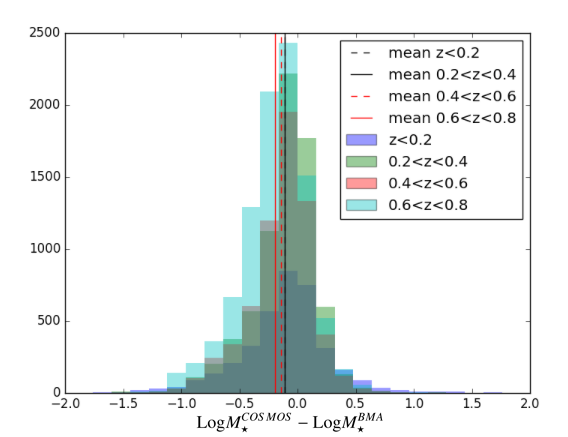
\includegraphics[width=0.7\textwidth]{./chapters/chapter2/figs/fig1.png}\caption{Comparison of galaxy stellar masses from \citet{laigle} using COSMOS data with those computed with the BMA algorithm using DES data in different redshift bins. The lines represent the mean value of the distributions. }\label{fig:cosmos}\end{figure}%delta_cosmos_chab.png

\subsubsection{Validation of the BMA method}
In order to test our method for stellar mass estimation, we use as reference a catalog that overlaps with DES observations and has been proven to provide robust stellar mass estimates. \citet{laigle} used \textsc{LePhare} to compute stellar masses with multiband data in 16 filters from UV to infrared over the $2~{\rm deg}^2$ COSMOS field. From this sample, matched to DES data, we cut all objects at $z=0$ to eliminate stars, and at $z>1.5$, as we do not expect DES to be able to estimate stellar masses beyond that value.  Galaxies with  $i$-band  magnitude above 23.0 are also cut out. The remaining sample comprises galaxies with $SNR>10$ in DES, for which we compute stellar masses using the BMA code and DES data. The bias distribution given by the difference in log galaxy stellar mass between the two samples ${\rm Log}(M_\star^{\rm COSMOS})-{\rm Log}(M_\star^{\rm BMA})$ is shown in Figure \ref{fig:cosmos}. Mean bias and scatter (that we quantify as the standard deviation of the distribution) are below the typical error on galaxy stellar masses from SED fitting ($\sim 0.2$ dex) in the redshift range $0.2<z<0.6$, where we expect good performance for optical surveys such as DES. At higher redshift, it is harder to constrain the optical to near-infrared (NIR) SED with the DES bands and therefore the scatter increases. Also at low redshifts ($z<0.2$), the 4000\AA~break is harder to constrain, as it is blue-ward of the $g$-band effective wavelength. The scatter will also be partially due to the fact that the COSMOS stellar masses are not ``true'' stellar masses, and will depend on the assumptions and methodology in \citet{laigle}. The slight bias that seems to exist in our DES stellar masses, particularly towards higher redshift, is probably due to the degeneracies between stellar mass and dust extinction. \citet{laigle} are able to constrain dust extinction better than in this work because of the information brought by the infrared data available to them.


\subsection{LePhare}

The main purpose of \lephare (PHotometric Analysis for Redshift Estimation) is to compute photometric redshifts by comparing template SEDs to the observed broadband photometry, but it can also be used to calculate physical parameters such as stellar masses and rest-frame luminosities. Several spectral libraries, both theoretical and empirical, are available within the code (including \citealt{cww}, \citealt{poggianti}, \citealt{bc03}), and these are redshifted and integrated through the instrumental transmission curves.  Additional contribution of emission lines in the different filters can be included and extinction by dust can be taken into account.  The synthetic colours obtained from the SEDs for each redshift are then compared to the data. The best fitting template and redshift for each object is then found by $\chi^2$ minimisation as described above for a generic template fitting method. In addition, prior information can be supplied, including a photo-$z$ distribution prior by galaxy type computed from the VVDS survey in the $i$ band (see \citealt{ilbertlephare}). 



\subsection{ANNz2}\label{sec:annz2}

\textsc{ANNz2} \citep{annz2} \footnote{\url{https://github.com/IftachSadeh/ANNZ}} is an updated version of the neural network code \textsc{ANNz} (\citealt{annz}). 
\textsc{ANNz2} differs from its previous version by incorporating several additional machine learning methods beyond Artificial Neural Networks (ANNs), such as Boosted Decision Trees (BDTs) and $k$-Nearest Neighbours (KNN) algorithms. 
These are implemented in the TMVA package (\citealt{tmva})\footnote{TMVA is a part of the ROOT C++ software framework (\citealt{root})}.

ANNs have been shown to have competitive performances for photo-$z$ estimation compared to other machine learning methods (\citealt{firth}), and therefore we use ANNs in the DES photo-$z$'s production. A neural network is made up of several layers, and each layer is composed by nodes. The number of nodes and layers depends on the chosen architecture. The inputs of the first layer are the observed magnitudes, colours, or any other galaxy property that could add information for redshift estimation. The output is the photo-$z$, or any other quantity that has been trained. In the \emph{multi--layer perceptron} method, which is implemented in \textsc{ANNz2} in ANN method, responses from each neuron of a layer are fed onto the following layer, and so on from input to output levels. Each response is fed with a weight, which is varied from cycle to cycle depending on the \emph{error function}, which quantifies the amount of error in predicting the output when compared to the target value.

The code can be run in a mode called ``randomized regression'', that allows to vary the input parameters of the chosen machine learning method. For example, when we use ANNs we usually randomly vary: the number of nodes in each layer, the number of training cycles, the usage of the so-called \emph{Bayesian regulator}, that reduces the risk of over-training, the type of activation function, the type of variable transformation performed before training (such as normalisation and PCA transformation) and the initial random seed.  After training is complete,  the performance of each method is quantified through an optimisation process, which leads to a single nominal photo-$z$ estimator for \textsc{ANNz2}. The entire collection of solutions is used in order to derive a $p(z)$, constructed in two steps.
First, each solution is folded with an error distribution, which is derived using the KNN error estimation method of \citealt{oyaizu}.
The ensemble of solutions is then combined using an optimised weighting scheme. This methodology allows us to take into account both the intrinsic errors on the input parameters for a given method, and the uncertainty on the method itself. %The methodology described above is what is called "randomised regression".
Another important feature implemented in ANNz2 is the weighting method (\citealt{lima}). It is therefore possible to give in input a reference sample and re-weight the training set to make its relevant variables distributions more representative of the former. \\


\section{Applications for cosmology and galaxy evolution}

\subsection{DES Science Verification photo-$z$'s}

\begin{figure}\centering 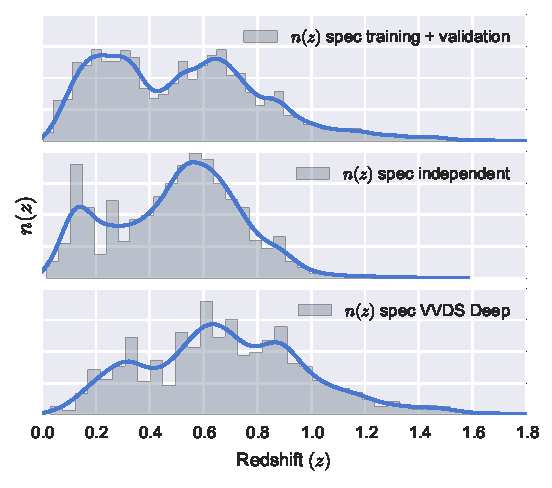
\includegraphics[width=0.6\textwidth]{./chapters/chapter2/figs/spec_distrubution_of_machted_cat.pdf}\caption{Redshift distributions (arbitrarily renormalised) of the spectroscopic sample used for training, validation and testing of DES SV photo-$z$'s. The top panel shows the distribution for training and validation samples, the middle panel for the independent testing sample from the VVDS F--14 field, and the the lower panel for an additional testing sample that goes to deeper magnitudes than the other fields (not mentioned in this work). From \citet{bonnett}.}\label{fig:specz}\end{figure}

In order to train ML methods and test their performance, we need a sample of galaxies with a measured spectroscopic redshifts that can be matched to DES photometry. This has been done in a comprehensive way within the DES photo-$z$ group for SV data, so that all algorithms would be trained and tested on the same sample. The final spectroscopic set comprises of $\sim 48,000$ galaxies spread over six fields in the sky, with measurements from 20 different surveys. This sample is split into training, validation and testing sample. In particular, the testing sample is independent from the training and validation sets in the sense that it comes from a separate field in the sky (the VVDS F--14), and thus its line of sight structure is uncorrelated from the other fields. This feature ensures that performance metrics evaluated on this sample would reveal redshift estimates that suffer from incompleteness of the training sample or that have been overtrained. Overtraining occurs when a ML algorithm becomes sensitive to fluctuations in the training data, rather than to actual features of the observables. This results in an apparent improvement of the performance metrics computed on the training sample, but it can be identified from a poorer performance on an independent testing sample. Overtraining can also be avoided through \emph{convergence tests}, which are available within the \textsc{ANNz2} code. These tests check whether the error estimator on training and validation samples have not improved over the last training cycles. The redshift distributions of the training, validation and testing samples are shown in Figure \ref{fig:specz}.

Several template fitting and machine learning methods have been used by the DES photo-$z$ working group on SV data. Four of them, namely \textsc{ANNz2}, \textsc{bpz}, \textsc{skynet} and \textsc{tpz}, have been used in \citet{bonnett} to estimate the impact of redshift distributions on cosmological parameters, in \citet{leistedt16} to infer the impact of spatial systematics on redshift distributions, and in \citet{SVkey} for cosmological analysis with cosmic shear.
I have used \textsc{ANNz2} to produce the photo-$z$'s used in these analysis and released at \url{https://des.ncsa.illinois.edu/releases/sva1}. The training has been performed in randomised regression mode for 100 ANNs, using as inputs the \texttt{MAG\_AUTO} magnitudes in $griz$ bands from the SVA1 gold catalogue. During training, the samples that we previously defined for training and validation are used. The testing samples is used to estimate metrics after the training is complete.

\begin{figure}\centering
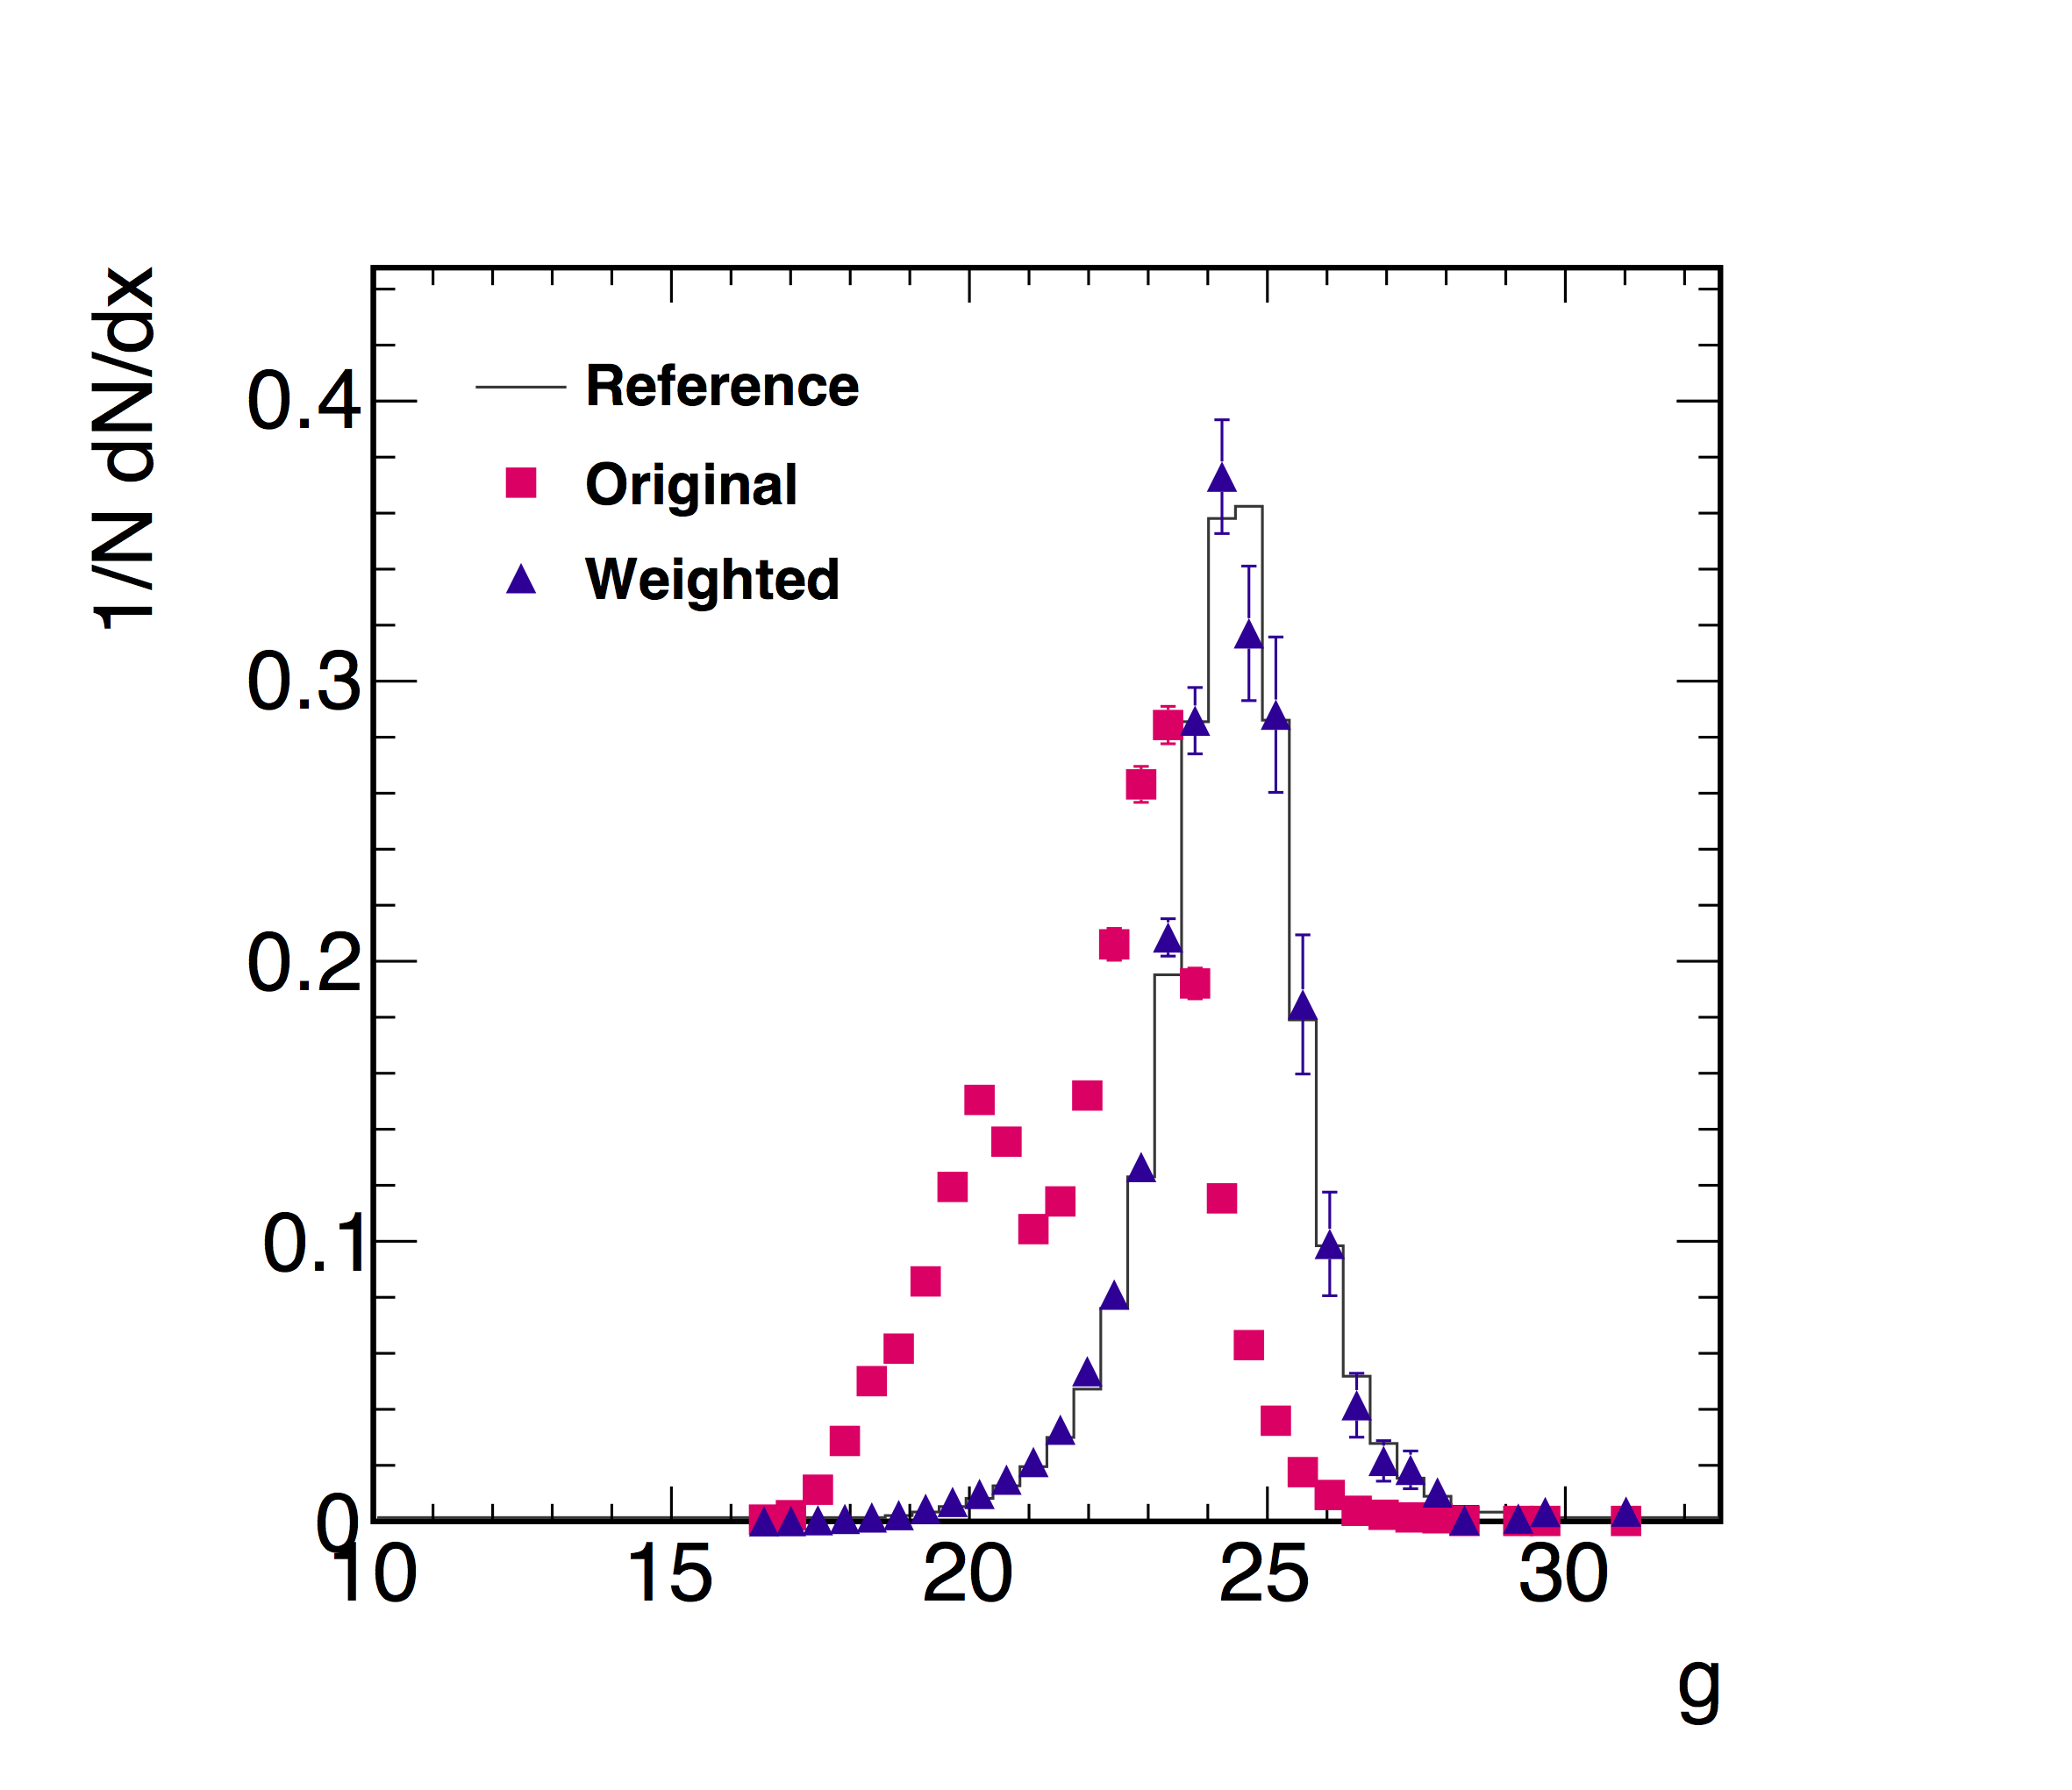
\includegraphics[width=0.4\textwidth]{./chapters/chapter2/figs/varWeightKNN_train_g.png} 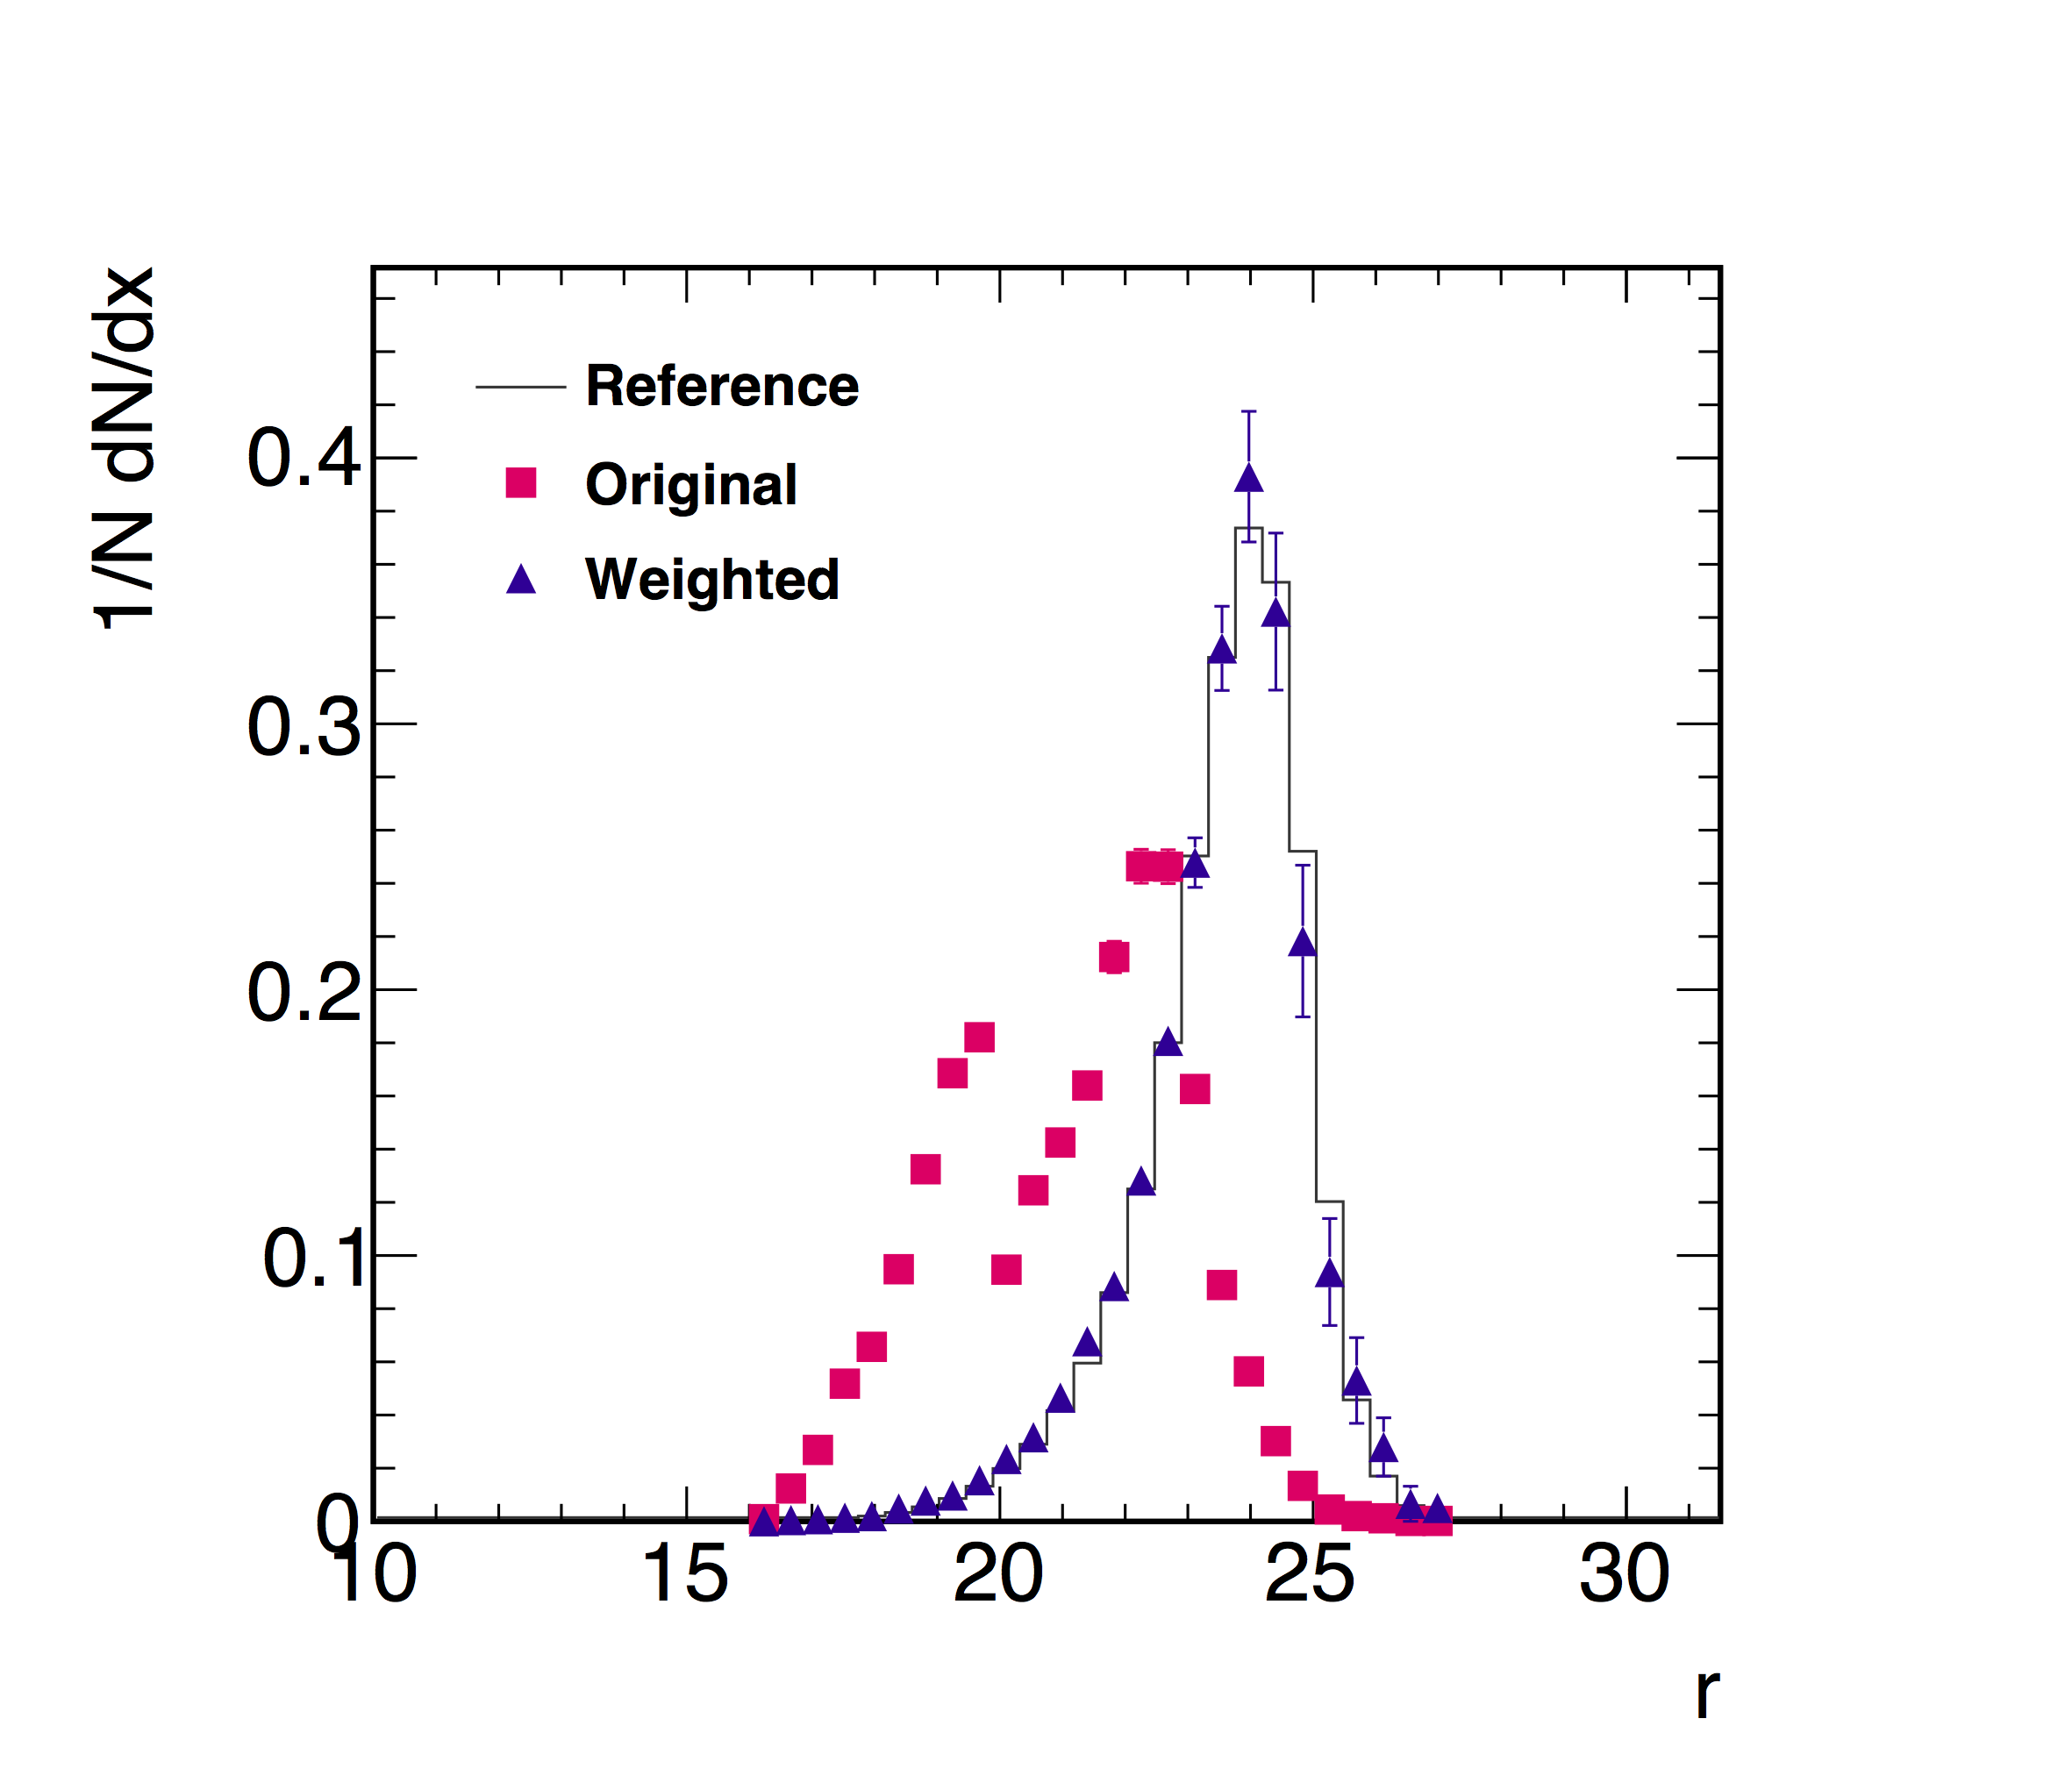
\includegraphics[width=0.4\textwidth]{./chapters/chapter2/figs/varWeightKNN_ANNZ_train_r.png}\\
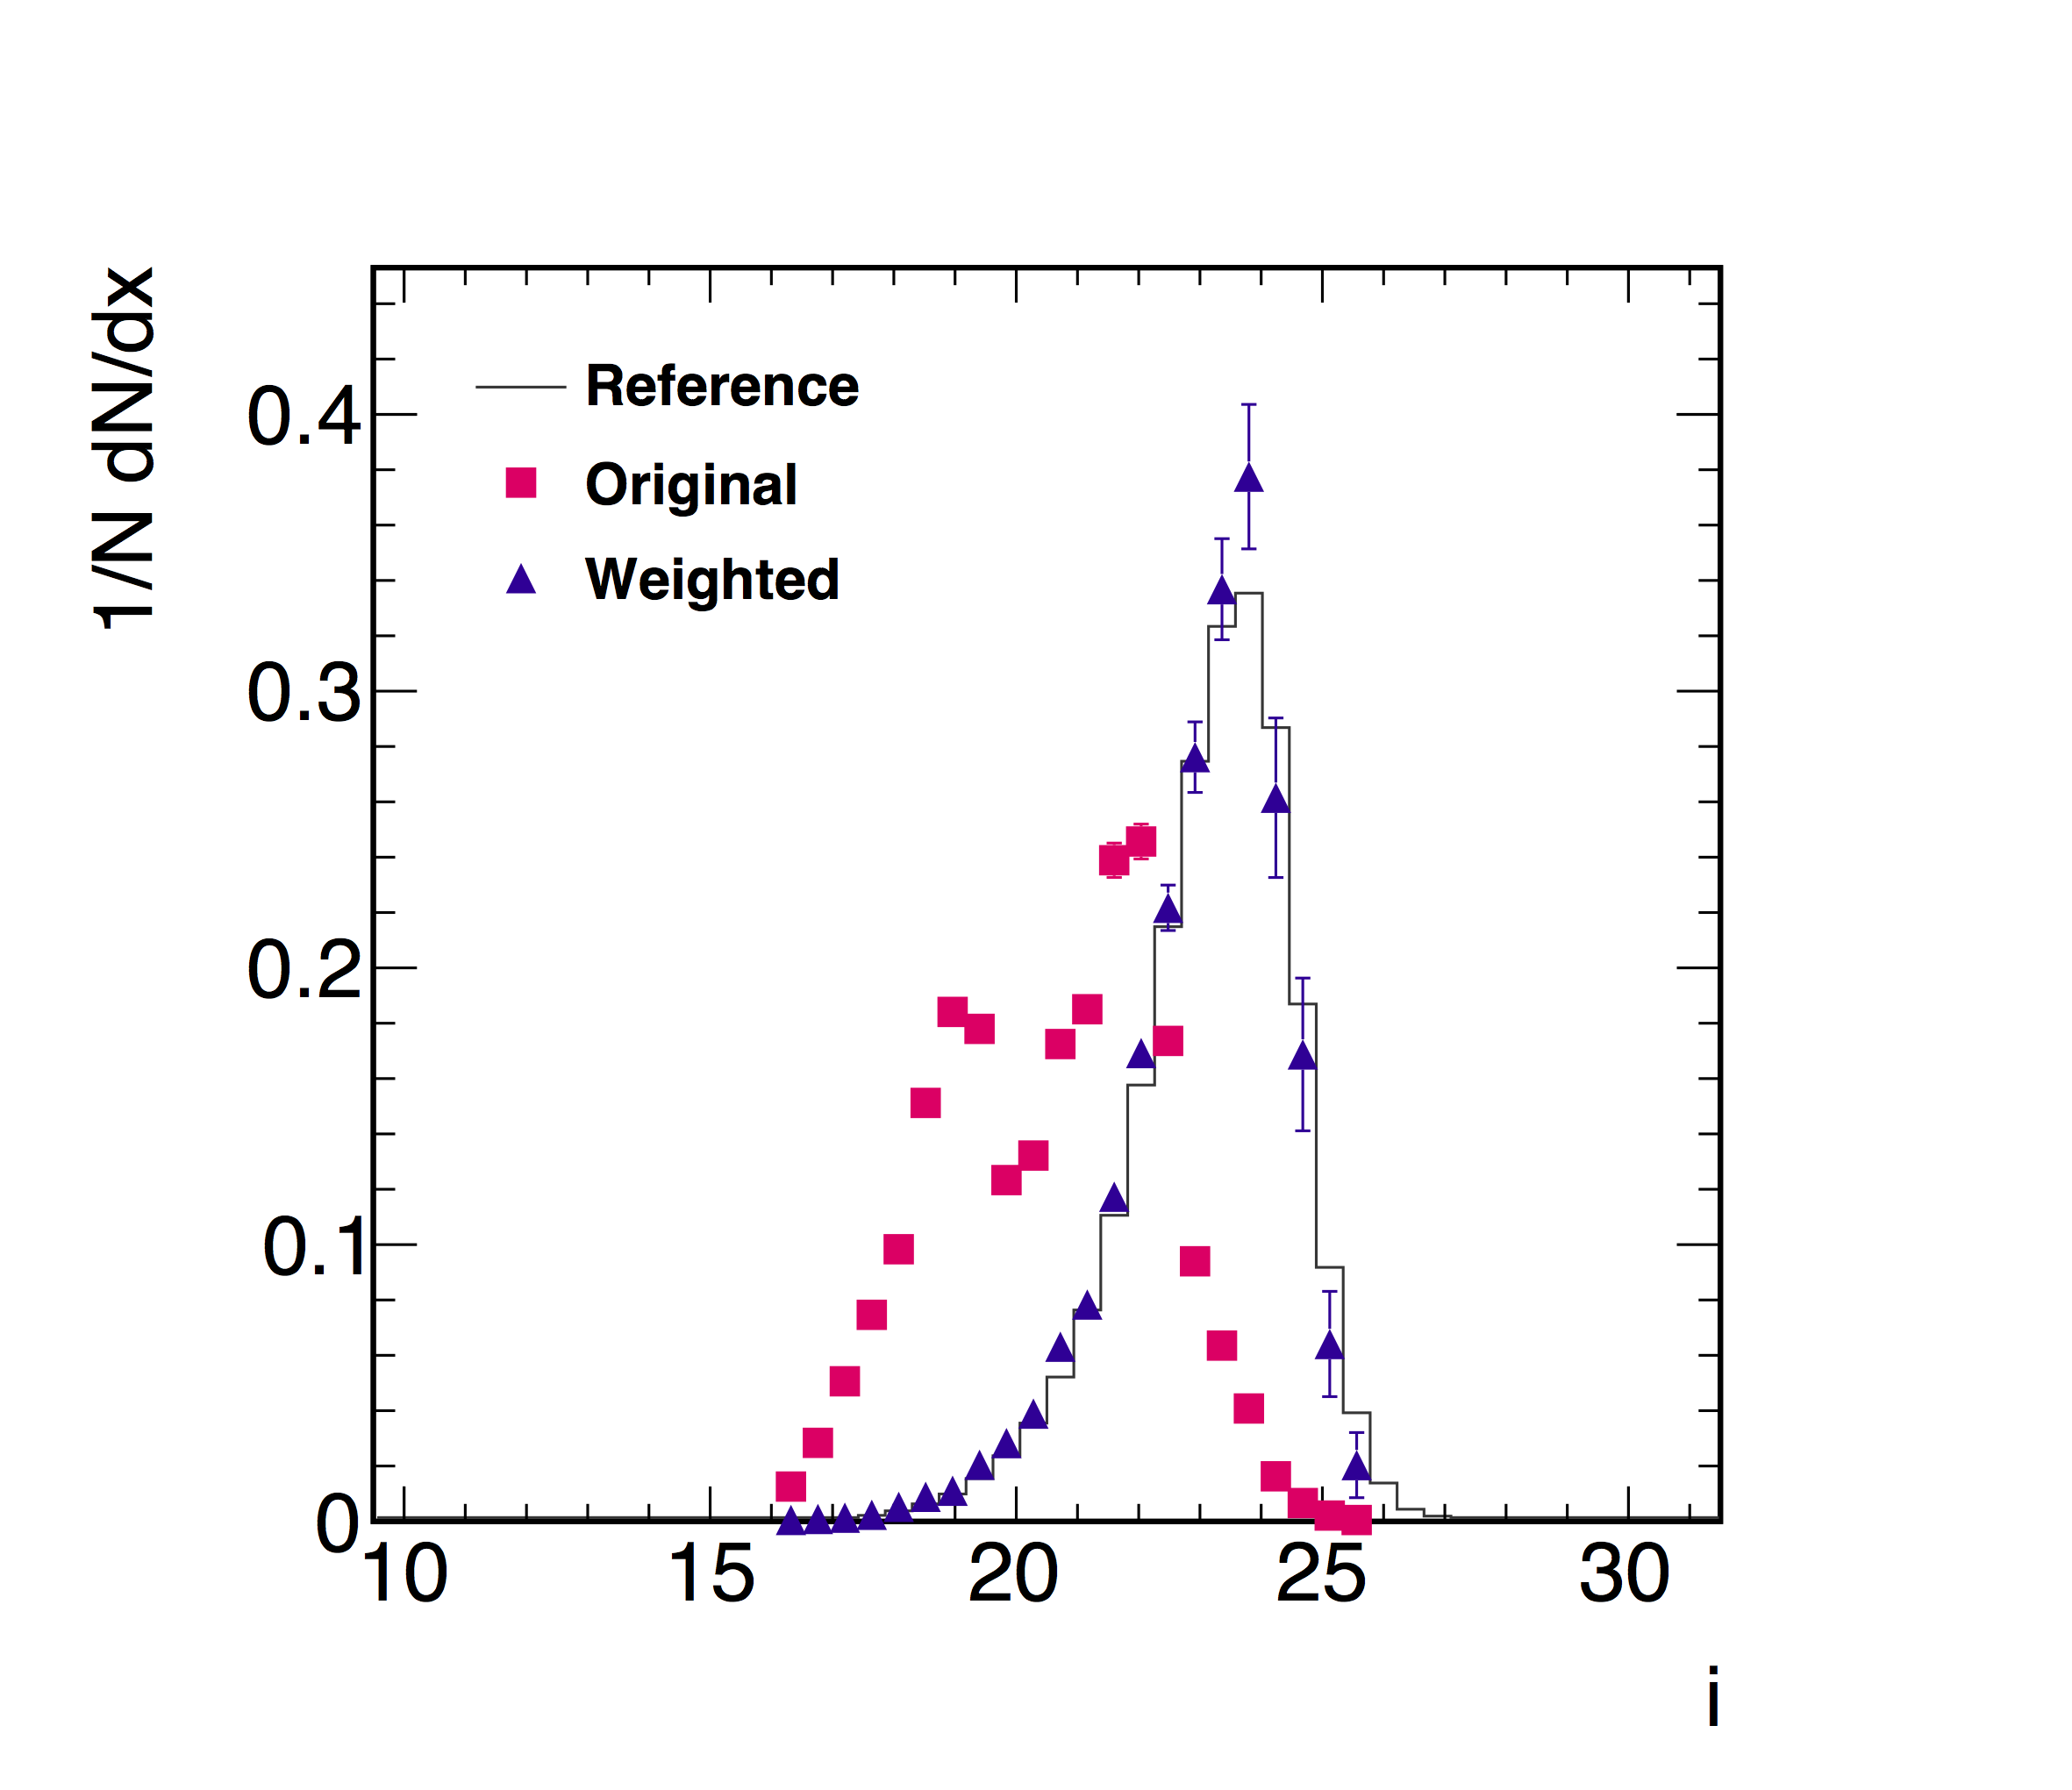
\includegraphics[width=0.4\textwidth]{./chapters/chapter2/figs/varWeightKNN_ANNZ_train_i.png} 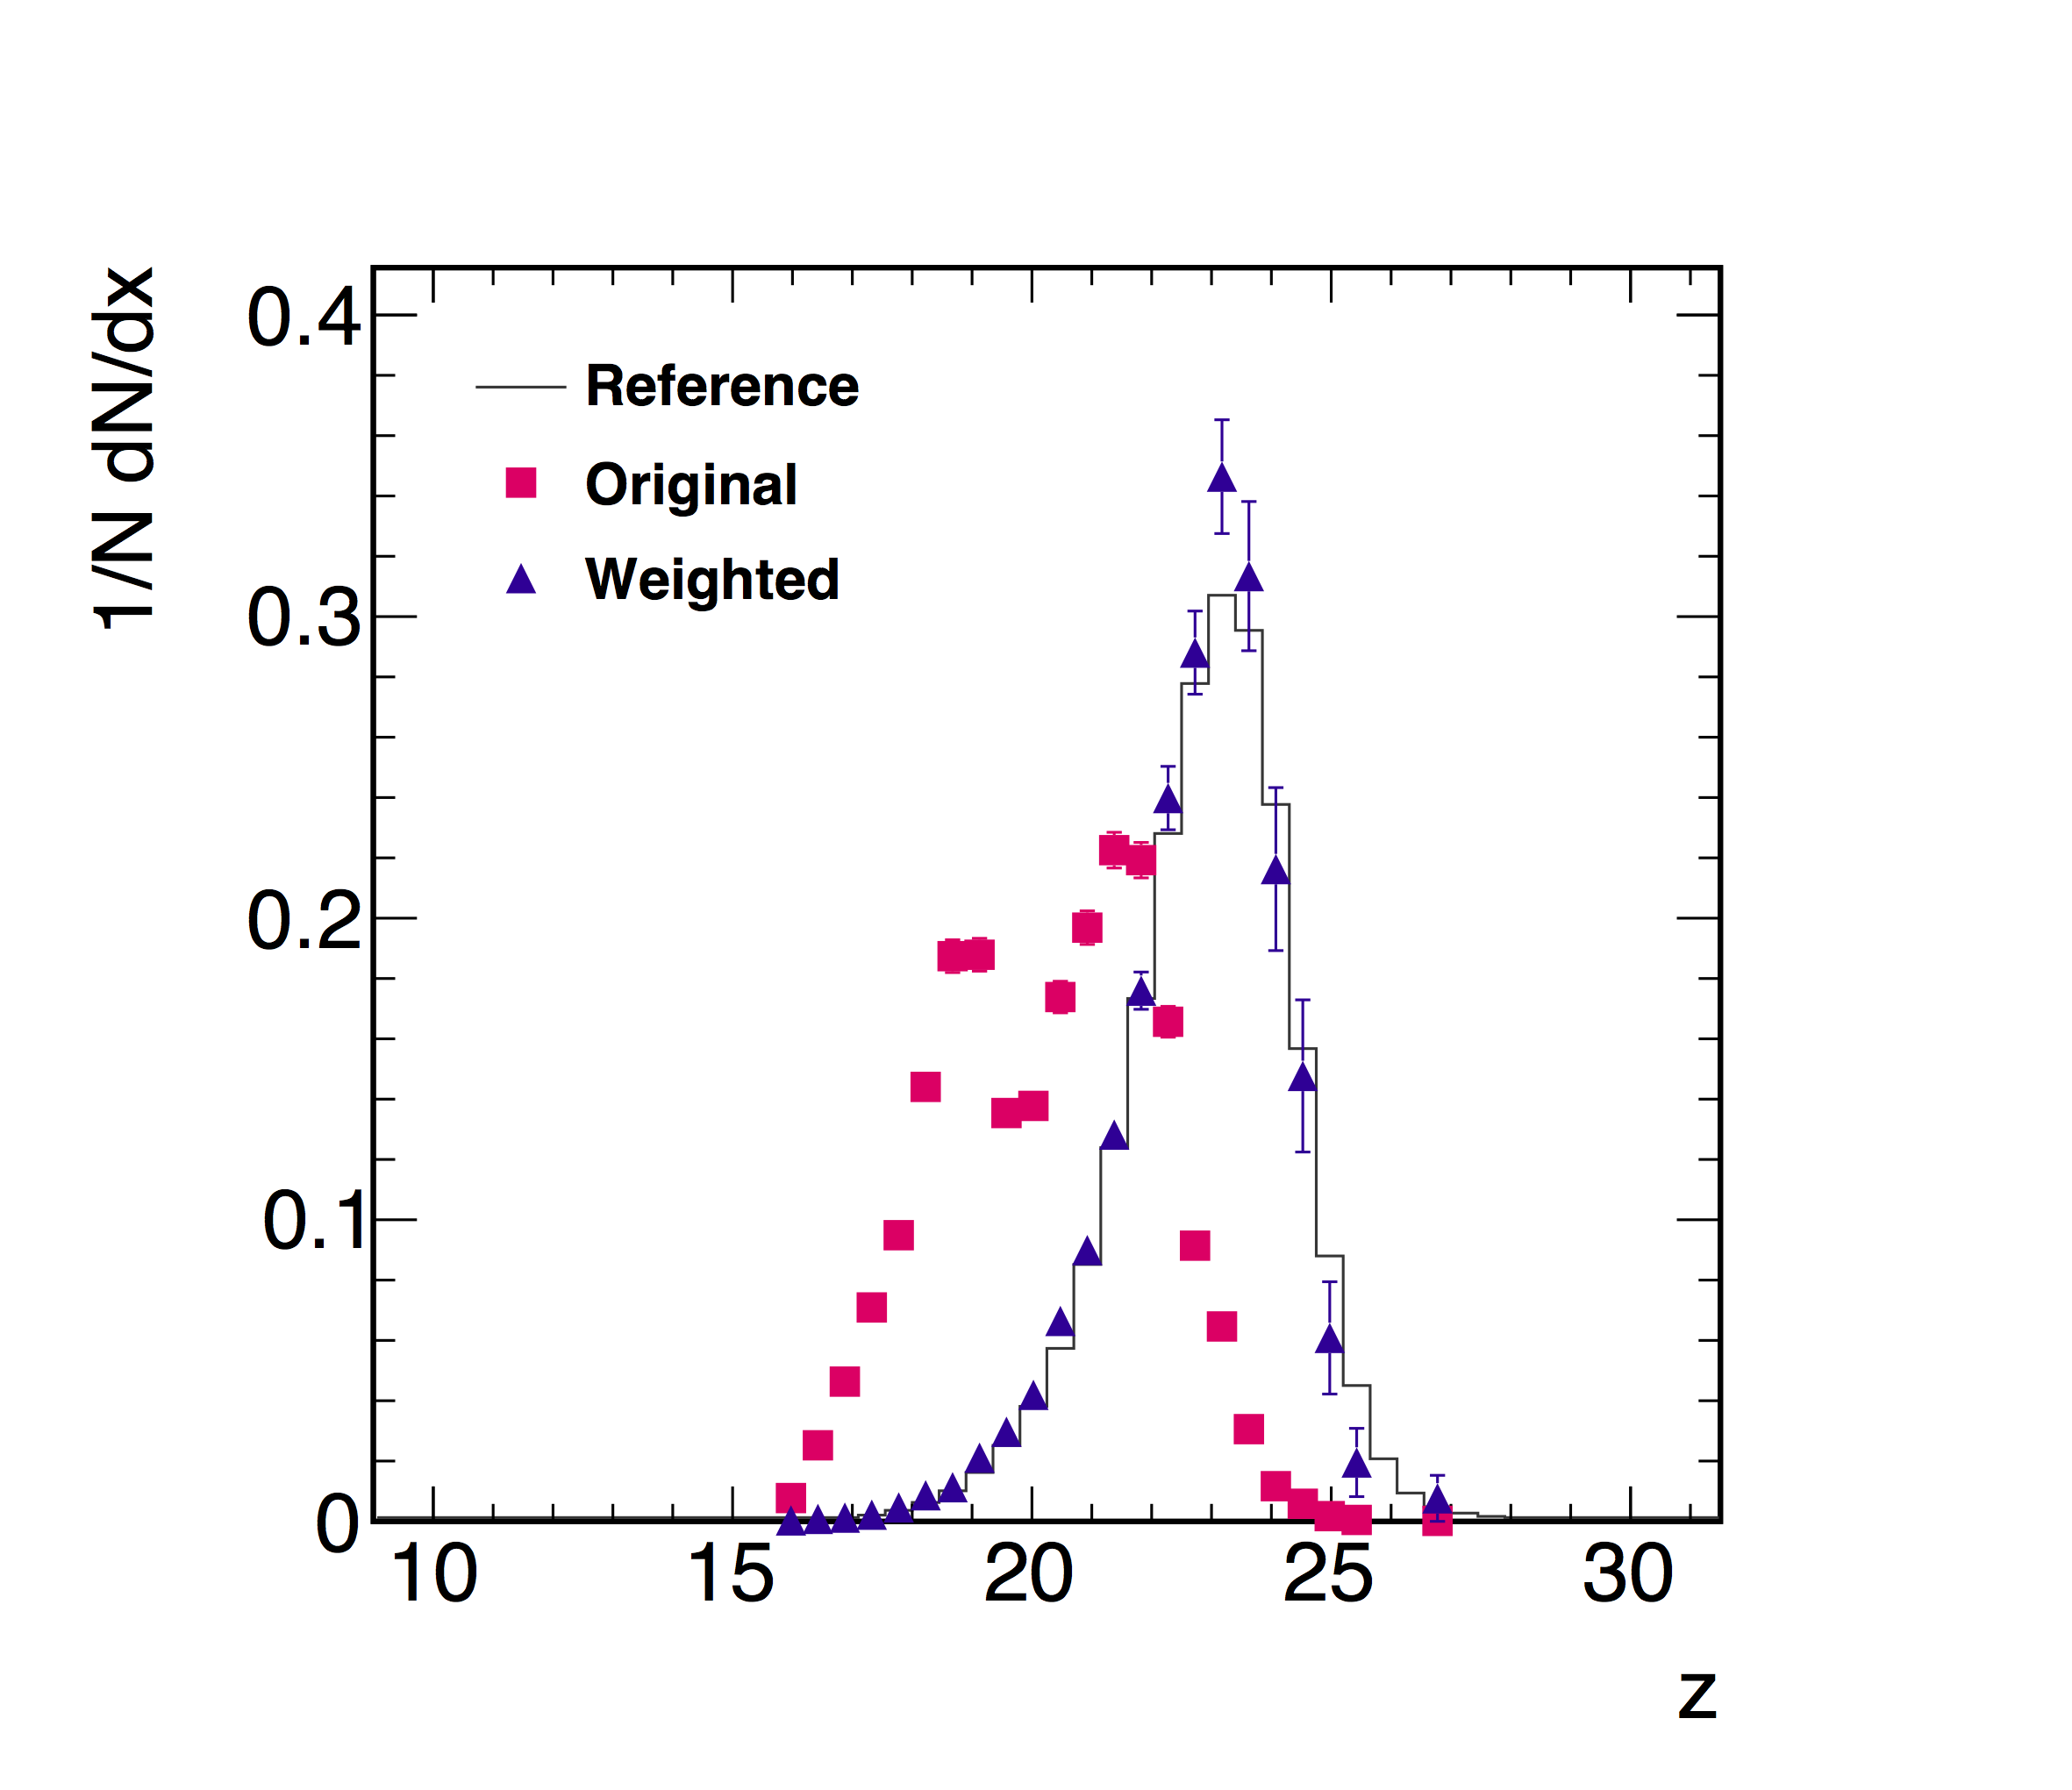
\includegraphics[width=0.4\textwidth]{./chapters/chapter2/figs/varWeightKNN_ANNZ_train_z.png}
\caption{Normalised distributions of the original magnitudes in $griz$ from DES photometry matched to the spectroscopic training sample (pink squares). The purple data points show the effect of the weighting method using as a reference sample SVA1 gold galaxy magnitudes (black histogram).}\label{fig:weight}\end{figure}

The weighting method mentioned in Section \ref{sec:zmethods} has been applied before the training. The key point of this method is to give more significance to training data which is representative of the population for which we want to compute the redshift. In Figure \ref{fig:weight} we show the original magnitude distributions from DES photometry matched to the spectroscopic training sample (pink squares). The purple data points show the effect of the weighting using as a reference sample SVA1 gold galaxy magnitudes (black histogram). It is clear how magnitude $\sim 19$ objects would have too high significance in the training. A correction factor is thus assigned to each galaxy depending on the input magnitudes. This is given by the number of neighbours in magnitudes--space in the training sample over the number of neighbours in the reference sample, both calculated within a set distance. Distances in magnitude space are simply Euclidean distances.

For this reason, dedicated catalogs need to be separately evaluated depending on the scientific analysis. We have produced dedicated catalogs for weak lensing and large scale structure (LSS) studies. The weak lensing catalog used for cosmic shear analyses typically has magnitude and redshift distributions comparable with the full gold samples for SV and Y1 releases. For example, the LSS Y1 sample is bright, as it has a sharp cut at $i<21$.

We have tested the use of the \texttt{inTrainFlag} computed within \textsc{ANNz2}. We provide this flag as part of our catalogs to identify galaxies that fall into incomplete regions of the training sample in the magnitude space. The photo-$z$'s associated with low values of this flag are found in underrepresented regions of the magnitude space, and thus their redshift is not reliable. Metrics have been computed on data and simulations as a function of this flag, and we find that a conservative cut that satisfies the DES requirements on bias and scatter is $\texttt{inTrainFlag}>0.7$. This flag, together with the weighting method, constitute our solution to incompleteness and unrepresentativeness of the training sample. 

Objects that have an unobserved band, have been treated as faint objects and considered at the mean magnitude limit for each filter (namely 24.67, 24.21, 23.78, 23.10 in $griz$). 

\begin{figure}\centering 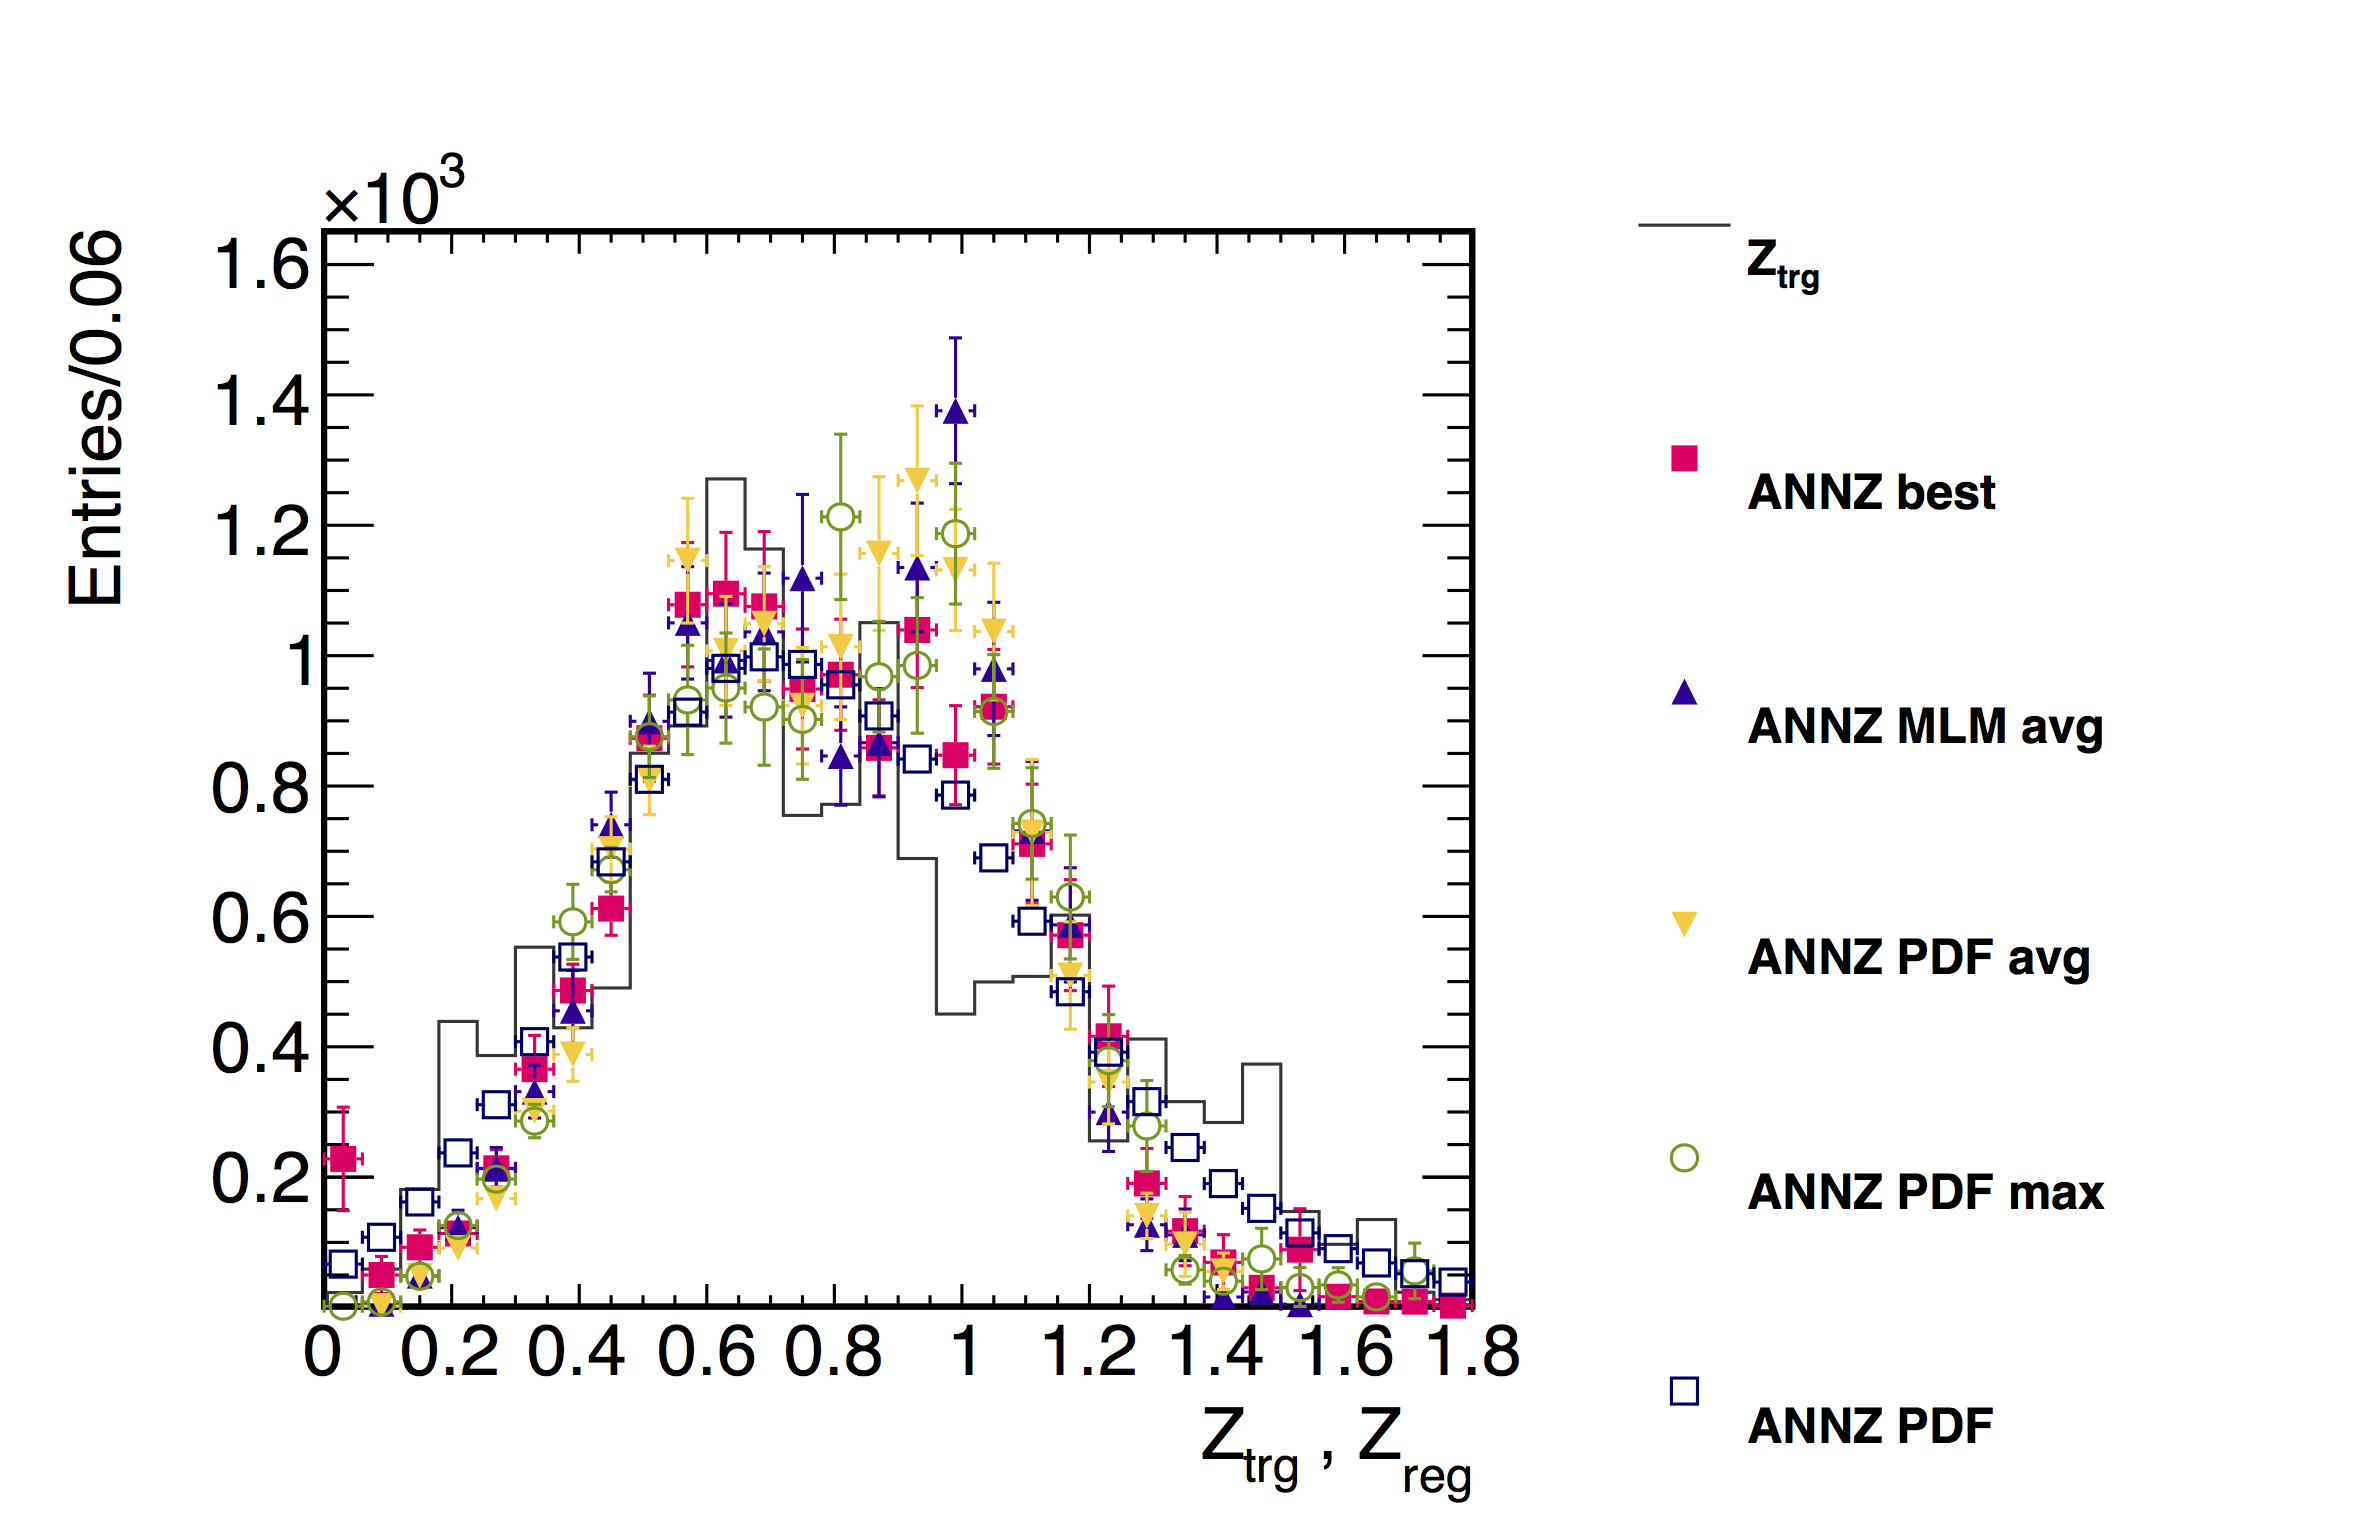
\includegraphics[width=0.8\textwidth]{./chapters/chapter2/figs/regTrgZ.png}\caption{Redshift distributions of the different \textsc{ANNz2} photo-$z$ estimators (coloured data points), compared to the target distribution from the weighted SV testing sample.}\label{fig:annznz}\end{figure}
\begin{figure} 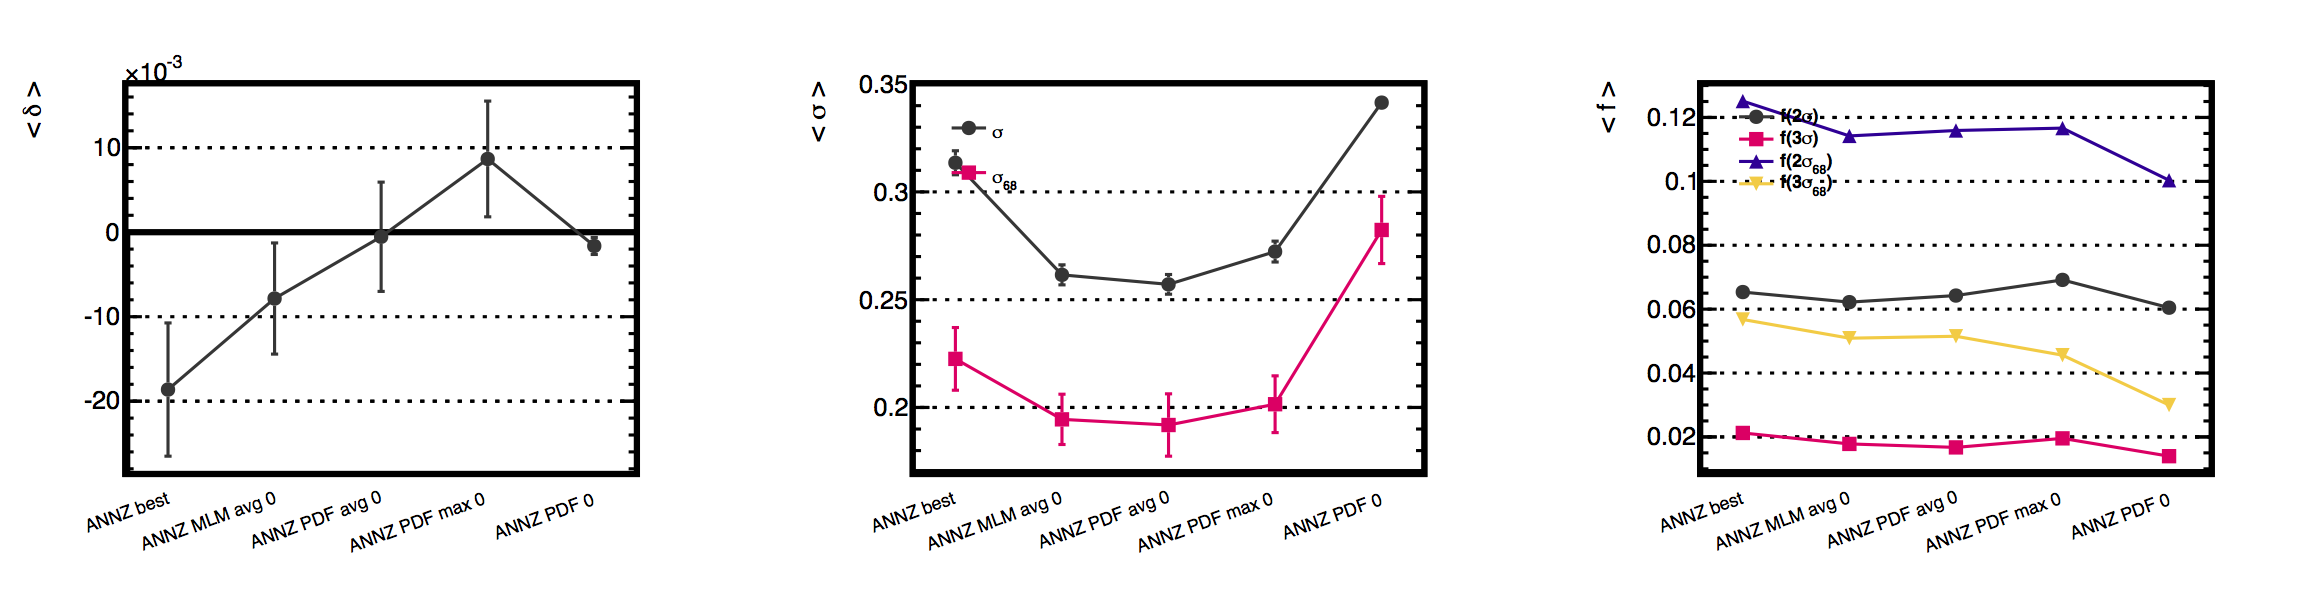
\includegraphics[width=1.05\textwidth]{./chapters/chapter2/figs/avgMetric.png}\caption{Performance metrics of the \textsc{ANNz2} estimators on the weighted testing sample. The metrics are, from left to right: bias, scatter (the standard deviation $\sigma$ and the 68th percentile $\sigma_{68}$ of the bias distribution) and outlier fraction. The outlier fractions are defined outside twice and three times the scatter values. }\label{fig:annzmetric}\end{figure}

Normalised redshift distributions and performance metrics on the testing sample for the different \textsc{ANNz2} redshift estimators are shown in Figures \ref{fig:annznz} and \ref{fig:annzmetric}, respectively. \texttt{ANNZ\_BEST} is the single--value solution from the ANN that performed the best out of the 100 ANNs, \texttt{ANNZ\_MLM\_avg} is the average of the solutions from all ANNs, \texttt{ANNZ\_PDF\_avg} is the single--value average of the full PDF solution, as computed from the randomised regression, and \texttt{ANNZ\_PDF\_avg} is the PDF maximum value. Based on the performance metrics, which are lowest in bias and scatter, we decide to use \texttt{ANNZ\_PDF\_avg} as the photo-$z$ nominal value.

\begin{figure}\centering 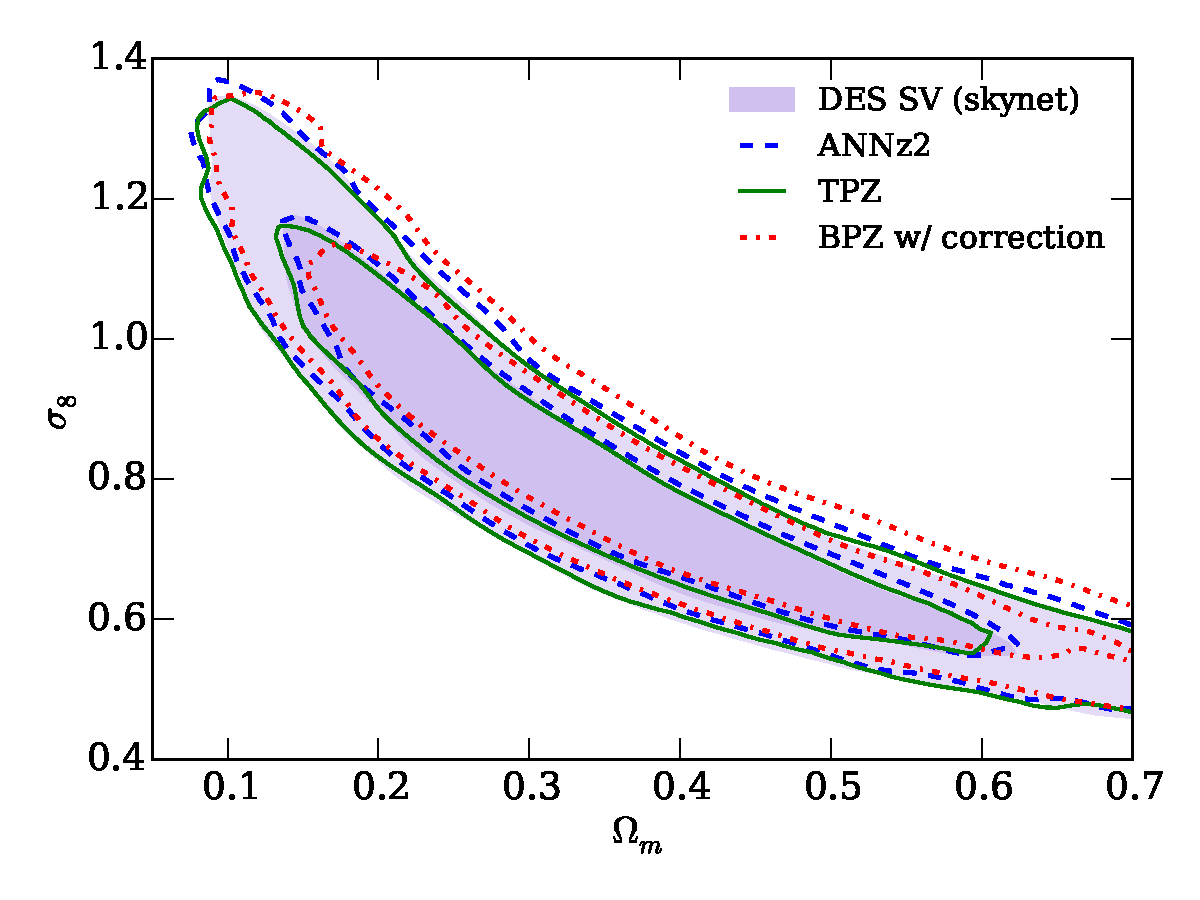
\includegraphics[width=0.7\textwidth]{./chapters/chapter2/figs/Om_sig8_nz.pdf}\caption{Impact of the photo-$z$ catalogue choice on the $\sigma_8$ and $\Omega_{\rm m}$ constraints. The constraints on $S_8$ computed from the different catalogues shift by less then two third of the errorbar. From \citet{SVkey}.}\label{fig:keySV}\end{figure}

\citet{SVkey} present the first cosmological constraints from DES SV data, using shear 2--point measurements over 3 redshift bins. They find $S_8\equiv \sigma_8(\Omega_{\rm m}/0.3)^{0.5}=0.81\pm0.81\pm 0.06$. Figure \ref{fig:keySV} shows the impact of the photo-$z$ catalogue choice on the $\sigma_8$ and $\Omega_{\rm m}$ constraints. Excellent agreement is found between the different codes, with the ML methods providing very similar results (note that they are trained on the same spectroscopic sample, and therefore they are not truly independent). \textsc{BPZ} is the only template fitting method presented, and it shows the largest difference compared to \textsc{SkyNet} (which is taken as the SV fiducial photo-$z$). However, in all cases the constraints on $S_8$ shift by less then two third of the errorbar.


\subsection{Stellar masses with machine learning}

In this subsection we present a new approach to derive galaxy stellar masses from multi-band photometric data using machine learning. 
It is faster by a factor of $\sim 100$ compared with standard template-fitting methods, and it allows to incorporate information from external higher quality data, therefore achieving similar, if not improved, performance.
Machine learning, which in this context can be viewed as an interpolation method, has been largely adopted in galaxies' redshift estimation, as outlined in the above, but has never been used to estimate stellar masses from photometric data.

\subsubsection{Method}
By using the \citet{laigle} COSMOS-based catalogue as a training set, which includes accurate stellar mass estimates based on a large number of broadband filters (see Section \ref{sec:BMA}), we train \textsc{ANNz2} using DES photometry. We use \textsc{LePhare} as a reference template fitting code, because this is also the method adopted by \citet{laigle} and this choice provides a fair performance comparison with ML.

The sample is cut in redshift, eliminating all objects at $z=0$ to remove stars, and at $z>1.5$, as the DES filter coverage does not typically allow to measure galaxy properties beyond this redshift. Galaxies with  $i$-band  magnitude above 23.0 are also removed. The remaining galaxies are matched to DES Year 1 photometry, which has $S/N>10$ after the selection cuts described. The training and testing samples are formed of $\sim 20,000$ galaxies with observed $griz$ bands randomly selected from the matched COSMOS-DES catalog. The rest of the catalogue ($\sim 20,000$ galaxies) is used for testing. 

The input variables provided to ANNz2 are DES \texttt{MAG\_AUTO} $griz$ magnitudes, and COSMOS photo-$z$'s. ANNz2 is run in single (i.e. only one ML method is run, with a single set of initial parameters) regression mode with BDTs, as ANNs run on this sample show biases due to a back propagation  issue: too much weight was allowed to be given to the redshift, that strongly correlates with the mass. % not enough controlled within TMVA, that allows weights to become too large. \footnote{In this case we believe too much weight was allowed to be given to the redshift, that strongly correlates with the mass.}

\begin{figure}\centering 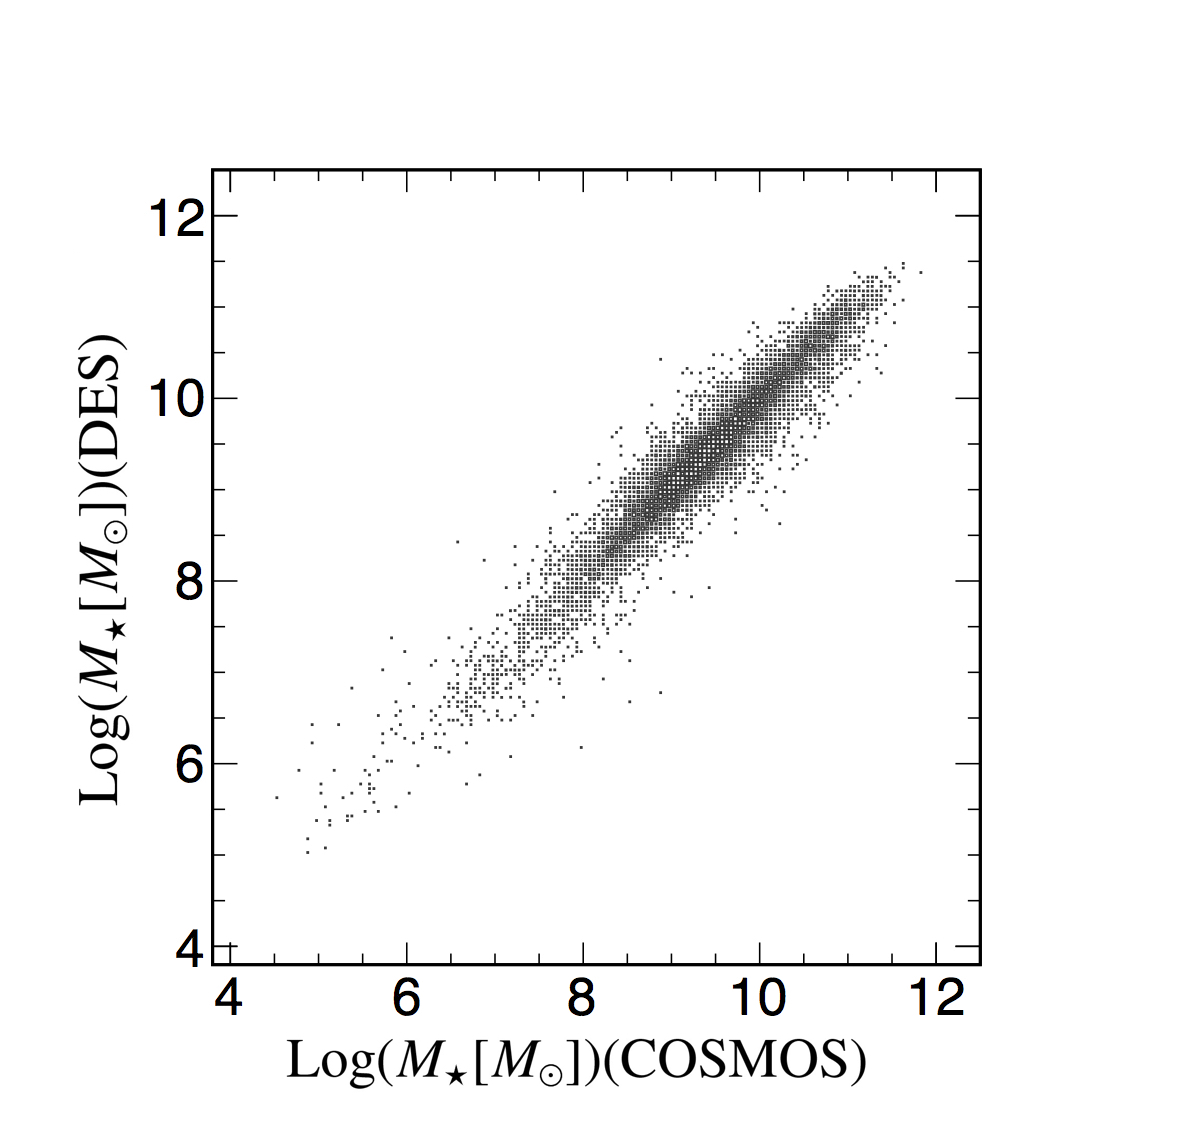
\includegraphics[width=0.7\textwidth]{./chapters/chapter2/figs/corRegTrgZ_ANNZ_best_MGcnvs.jpg}\caption{Stellar masses computed with boosted decision trees using DES 4--bands photometry, compared to the COSMOS stellar masses from \citet{laigle} evaluated with \textsc{LePhare} and 16--filters photometry. The COSMOS stellar masses represent our `true'' values in the testing sample shown here.}\label{fig:m_vs_m_bdt}\end{figure}

The template fitting evaluation was performed with \textsc{LePhare} and a set of 20 SPS templates from Bruzual \& Charlot (2003). The templates were chosen in order to be as similar as possible to the set used in \citet{laigle}. 

\subsubsection{Results}
The stellar masses estimated with \textsc{LePhare} show a mean of the bias distribution of $\bar{\Delta}=-0.051\pm 0.002$ dex and a scatter $\sigma = 0.32\pm 0.01$ dex on the testing sample. A single random forest run with ANNz2 has $\delta=-0.006\pm 0.001$ and $\sigma=0.31\pm 0.02$ dex. A comparison with the COSMOS catalogue masses (i.e. our ``true'' values in the testing sample) is shown in Figure \ref{fig:m_vs_m_bdt}. The performance is very similar, even with a lower bias from ML estimates. Given that the template fitting was performed in an almost identical fashion as in \citet{laigle}, we believe that the higher bias is due to a lack of filters in the DES data compared to COSMOS. Machine learning techniques show a better control as they are able to incorporate information from the COSMOS data through training. Computing times are $\sim 100$ times quicker with ANNz2 than with \textsc{LePhare}, providing an ideal method to compute stellar masses in a binned range of redshift, and obtain in a reasonable time full stellar mass PDFs.
The idea behind this approach is that ML acts as an interpolation method between the different stellar population synthesis models, and can ``learn'' quickly prior information contained in more sophisticated photometric or spectroscopic surveys.

Further tests of this method concern the inclusion of morphological parameters in the input variables. \citet{soo} show that there is room for improvements on photo-$z$ estimation when morphological information is added to photometric data from less than 5 bands. We therefore utilise morphological and photometric information from Multi-Object Fitting (MOF) pipeline that uses the \texttt{ngmix} code\footnote{\url{https://github.com/esheldon/ngmix}} available for the same galaxy sample used here. However, we find that the inclusion of galaxy size and light profile type (through the MOF outputs \texttt{T}\footnote{The size squared of the object.} and \texttt{fracDeV}\footnote{In the MOF composite model, the light profile is fit to a de Vaucouleurs plus exponential model. The fraction of the light profile which follows a de Vaucouleurs profile is given in \texttt{fracDeV}.}) does not improve upon the performance. A $\sim 20\%$ improvement on the bias is found only thanks to the improved MOF photometry when compared to the SExtractor \texttt{MAG\_AUTO} magnitudes. %We have also found that removing the photometric redshift from the input parameters does not worsen the metrics withi

We conclude that this approach to stellar mass computation is promising, and we have computed a first catalog for DES Year 1 data using this method. Assuming BPZ photo-$z$'s and MOF photometry, we recovered stellar masses over the Y1 wide field footprint of $\sim 1,800$ sq. deg., shown in the mass map in Figure \ref{fig:massmap}. Future work will use a cross--correlation of stellar mass maps with weak lensing maps to constrain the stellar--to--halo mass relation.

\begin{figure}\centering 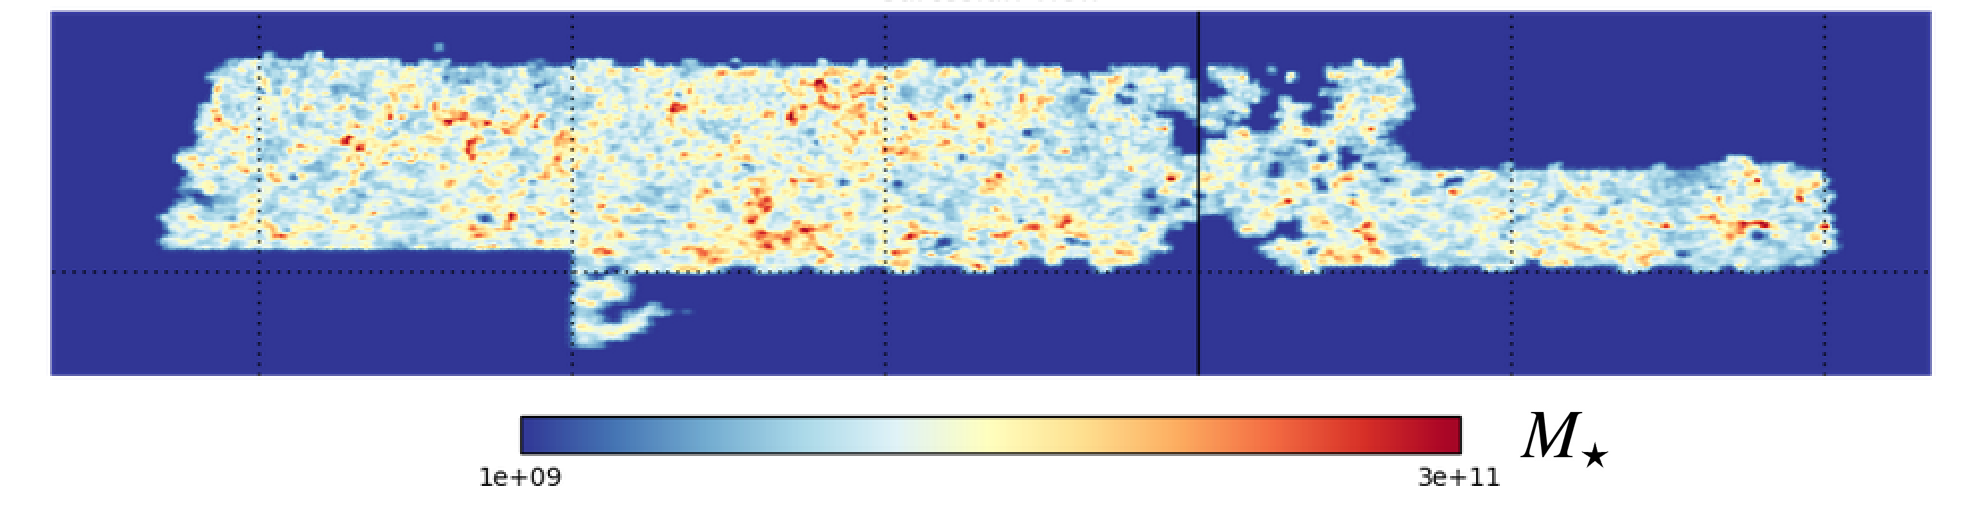
\includegraphics[width=1\textwidth]{./chapters/chapter2/figs/smass_map.png}
 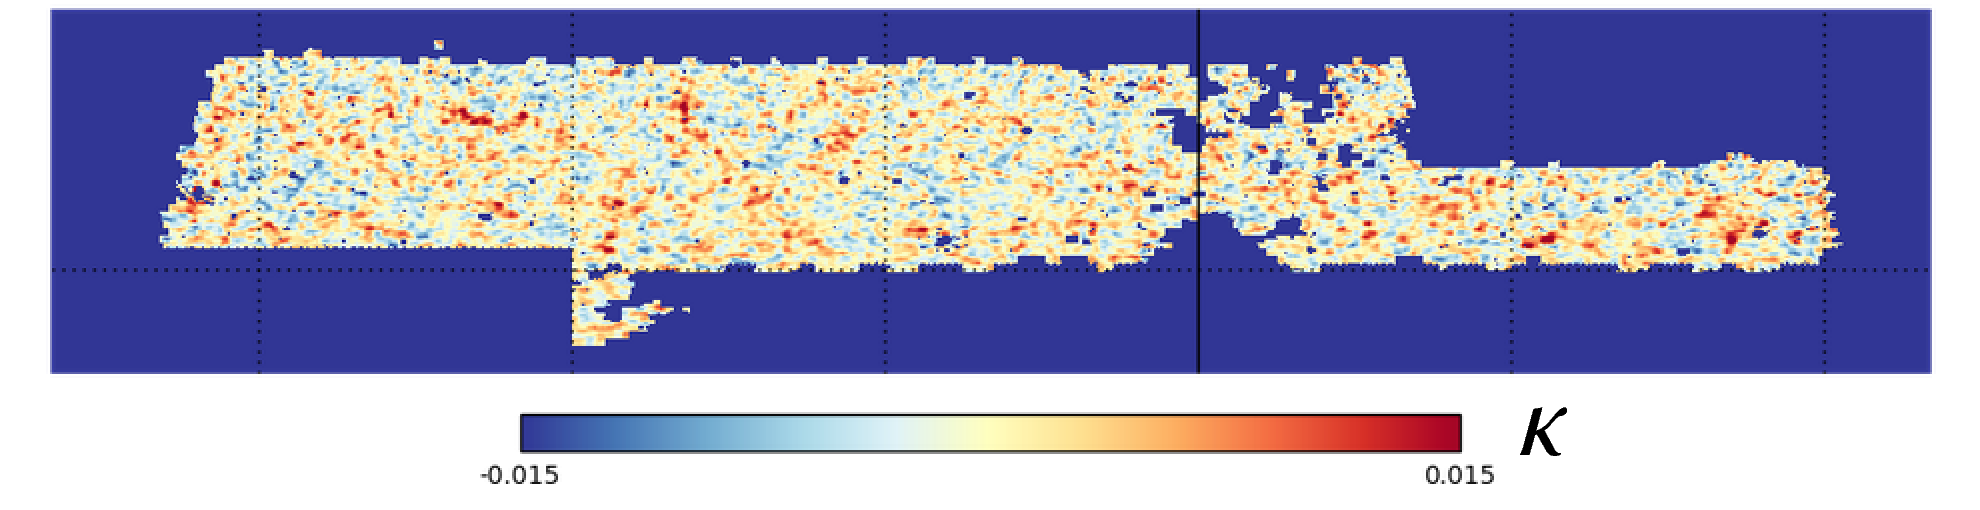
\includegraphics[width=1\textwidth]{./chapters/chapter2/figs/wl_mass_map.png}
\caption{\emph{Top:} Stellar mass map over the DES Year 1 wide field. It comprises galaxies with redshift $0.2<z<0.4$. \emph{Bottom:} Weak lensing convergence $\kappa$ mass map by \citet{2018MNRAS.475.3165C} for sources at $0.6<z<0.9$ (E modes). The cross--correlation of this mass map with the stellar mass map of foreground galaxies produces a signal which can be used to study the stellar--to--halo mass relation.}\label{fig:massmap}\end{figure}


\section{Conclusions}

In this Chapter, we have reviewed the basic concepts behind photometric redshift estimation and galaxies' SED modeling. The SED fitting techniques used in this thesis have been described. We have then shown some applications of the methods to DES data. In particular, we have described how the ANNz2 photo-$z$'s catalogue for the DES SV release has been produced, and how machine learning can be applied to DES data for stellar mass estimation. The approach presented allows to incorporate information from external higher quality data, and achieving similar, if not improved, performance compared to traditional methods. The method is also significantly quicker than others ($\sim 100$ times quicker than \text{LePhare}), which is useful when dealing with large photometric surveys such as DES, and we predict that it will allow us to produce full stellar mass PDFs in a reasonable time.

In future analyses, we plan on studying cross--correlations of stellar mass maps, computed with machine learning techniques on DES Year 3 data, with weak lensing mass maps. By predicting a convergence mass map, which can be defined by an adaptation of \citet{2016ApJ...833..156U}, from our observed ``stellar convergence'' $\kappa_*$ map, we will fit a stellar--to--halo mass relation to weak lensing observations. This measurements will provide insights on the distribution of stellar matter relative to dark matter, and on the relative contribution of these components also outside galaxy clusters (which are discussed in Chapter 6).












\clearemptydoublepage
\chapter{Host galaxies for gravitational wave follow ups and the case of GW170817}\label{chp:chp3}

\begin{flushright}
  {\em ``Open your eyes, look up to the sky, and see''}\\
\ \
\normalsize
{Queen}  
\end{flushright}

\noindent \emph{The work presented in this Chapter is an extended version of ~{\bf Palmese et al. 2017, ApJ 849L, 34P}, with some information from the GW170817 DECam discovery paper {\bf Soares--Santos et al. 2017, 848, L16} and work done as part of the DECam--GW follow up program yet to be published. The DECam--GW pipeline is shortly described in Herner et al. 2017 and has been used in the GW170814 analysis by Doctor et al., in preparation. I am an author or co-author in all of the works listed above. Some information from the earlier work on DECam GW follow ups are also presented (from \citealt{marcelle16} and \citealt{Cowperthwaite16}). }\\

\noindent The first identification of the electromagnetic counterpart \citep{MMApaper} of a gravitational wave (GW) signal \citep{ligobns} marks the beginning of a new era for multi-messenger astronomy. More than 3000 physicists and astronomers from all around the globe probed every aspect of the event, across the electromagnetic spectrum and into the realms of gravity theories and particle physics. Amongst the several expected transients described in Chapter \ref{chp:chp1}, the coalescence of neutron stars is expected to have strong optical and near-infrared signatures in the form of a kilonova, the ejecta from which are heated by the decay of heavy nuclei produced via $r$-processes. The optical counterpart to the BNS coalescence signal GW170817 was discovered independently by several collaborations using optical telescopes, including the Dark Energy Camera GW team \citep{marcelle17}. 

In this Chapter we exploit galaxy catalogs for follow ups of gravitational wave events, focusing on the follow up of the DECam golden event GW170817. We show how deriving properties of galaxies, including redshifts, stellar masses and star formation rates, from photometric and spectroscopic surveys can boost our GW EM follow up strategy and understanding of GW sources. We start by presenting the DECam--GW follow up program in Section \ref{sec:desgw}, focusing on the galaxy host matching of candidates which has been my main task within the follow up effort. In Section \ref{sec:gw170817} we describe a study of NGC 4993, the host galaxy of the GW170817 GW event, the GRB170817A short gamma--ray burst (sGRB) and the AT2017gfo kilonova. We use Dark Energy Camera imaging, AAT spectra and publicly available data, relating our findings to binary neutron star (BNS) formation scenarios and merger delay timescales. NGC4993 is a nearby (40 Mpc) early--type galaxy, with $i$-band S\'ersic index $n=4.0$ and low asymmetry ($A=0.04\pm 0.01$). These properties are unusual for sGRB hosts. However, NGC4993 presents shell--like structures and dust lanes indicative of a recent galaxy merger, with the optical transient located close to a shell. We constrain the star formation history (SFH) of the galaxy assuming that the galaxy merger produced a star formation burst, but find little to no on--going star formation in either spatially--resolved broadband SED or spectral fitting. We use the best--fit SFH to estimate the BNS merger rate in this type of galaxy, as $R_{NSM}^{gal}= 5.7^{+0.57}_{-3.3} \times 10^{-6} {\rm yr}^{-1}$. If star formation is the only considered BNS formation scenario, the expected number of BNS mergers from early--type galaxies detectable with LIGO during its first two observing seasons is $0.038^{+0.004}_{-0.022}$, as opposed to $\sim 0.5$ from all galaxy types. Hypothesizing that the binary system formed due to dynamical interactions during the galaxy merger, the subsequent time elapsed can constrain the delay time of the BNS coalescence. By using velocity dispersion estimates and the position of the shells, we find that the galaxy merger occurred $t_{\rm mer}\lesssim 200~{\rm Myr}$ prior to the BNS coalescence. 
Note that in this work we may use the word ``merging'' for both the galaxy merging and the binary coalescence.


\section{Gravitational wave follow up with DECam}\label{sec:desgw}

A subset of GW events are expected to produce an electromagnetic (EM) emission that once detected, can provide information complementary to the waveform. Observing the EM counterparts offer a number of exciting scientific opportunities for cosmology, astrophysics and physics of the space--time, as we have described in Chapter \ref{chp:chp1}. It is worth stressing that follow ups of BBH events are interesting even though most accepted BBH merger models do not predict an EM counterpart, as they lack the massive accretion disks expected to produce GRBs and other observable transients (e.g. \citealt{2016arXiv160909517A} and references therein). However, there exist theoretical models that could produce an EM signal (e.g. \citealt{loeb}, \citealt{demink}): these are highly speculative, and assume the presence of matter around the binaries in the form of circum--binary disks, or mergers happening within another star. There are three (not mutually exclusive) reasons for non-detections: (1) the probable sky regions of previous BBH detections were not searched comprehensively, (2) the BBH emission could not be distinguished from background transients, and/or (3) emission from BBH mergers is below the detectable threshold of current instruments. The possibility of (1) and (2) implies that detectable BBH emission cannot yet be ruled out, and placing upper limits on the emission provides interesting constraints on theoretical models of BBH mergers.

With these benefits in mind, the LVC established partnerships with several collaborations around the globe, including DECam. Shortly after their first analysis of the GW signal, LVC shares with the partner collaborations a number of useful information, including the estimated distance to the source, the type of event (BBH, BNS, BH+NS mergers) and a map of the probability for the source of the event to be located in different positions of the sky. The LVC trigger information are communicated through a private network to the EM follow up partners, similarly to what is used in the gamma--ray community. The partner collaborations then decide whether to follow up the candidate, depending on factors such as the observability of high probability regions of the skymap from their telescope. Our EM follow up group consists mainly of DES members, and some external collaborators from the astronomical community, so that the program was named DECam--GW program. At present, DES is one of the primary users of DECam, and the DECam--GW team obtained $\sim 4$ nights of telescope time per year over the past two observing seasons, to be added to the DES allocation of $\sim 105$ nights per year. When a LVC trigger is received, the team uses dedicated observing strategy codes to decide whether to observe the event. If the decision is positive, DES observations are interrupted to start the follow up. The LVC might update their analysis of the event later on, resulting in a new skymap. If this happens while the follow up observations are still on, we modify our observing strategy accordingly.

\subsection{Observing strategy}
The observing strategy is mostly optimised to catch the EM emission expected from BNS merger models. These predict that the EM counterpart will fade in a matter of days to a week time from the GW trigger. It is therefore crucial to quickly identify, analyse and eventually report candidates for further photometric and/or spectroscopic follow up. Clearly, DECam represents a premier instrument in the Southern emisphere to achieve these goals, given its wide and unique field of view. A general rule is to observe candidates three times: once as soon as possible after the trigger, 2 or 3 days later and about two weeks later, in order to observe the decline in flux of potential kilonova events. The first steps in planning the observations once the trigger is received consist in (i) produce $10\sigma$ limiting magnitude maps for the following 24 hours for 90 seconds exposures, (ii) calculate source detection probabilities for those maps and (iii) select pointings to be observed based on these probabilities. This is done for time slots of $\sim 1/2$ hour. The source detection probabilities are computed given the limiting magnitudes from (i) and a source model. At present, we do not have a realistic model for BBH EM and we just assume that the source has an apparent magnitude of $i=20$. The kilonova model used for BNS and BH+NS events is a modified version of the model by \citet{barneskasen}. The detection probability maps are divided into DECam pointings, and time slots of roughly half an hour containing an integer number of pointings are created. The exposures are taken in $i-$band for BBH follow up and in an $izz$ sequence for NS mergers, given that we expect kilonovae to emit in the optical--near infrared. This is done for all available time slots, and it is repeated for the following available nights.


\subsection{Image processing}
Once the images have been taken, they are processed through the difference imaging pipeline, initially developed for supernovae searches with DES by \citet{herner}. Supernova light curves are typically very similar to what we expect a kilonova to look like from our DES photometry, just bluer and brighter. It is thus natural to borrow some methods from SN searches. The difference imaging consists in subtracting from the new follow up images the ``templates'', which are DECam images of the same area of the sky taken previously to the event. We search for new objects in the residual images obtained, which constitute our potential candidate transients. This pipeline is able to use as templates partially overlapping exposures, and also publicly available images taken with DECam outside of the DES allocated time. In particular, part of us in the DES-GW team are also involved in the BLanco Imaging of the Southern Sky (BLISS), a dedicated program aimed at providing templates in the whole observable southern sky (along with other science cases). BLISS has already observed 1000 ${\rm deg}^2$ of the DECam observable sky in $griz$ which had not previously been covered.

\subsection{Post--processing}

After the images have been processed, we assess the outputs and create a candidate list to analyse. An important step consists in rejecting non--astrophysical artifacts that may arise from the difference imaging, for example close to CCD edges. This is achieved by classifying the candidate transients through a machine learning method that assigns a score between 0 (high probability of being an artifact) and 1 (high probability of being a real object). So far in the analyses we have assumed a cut in the score at $\geq 0.7$, where the efficiency of this cut was measured from point sources injected into our images to be $\gtrsim90\%$ in both $i$ and $z$ up to $z=22$. Depending on the type of event, one may want to apply other cuts to the list of transients. The next step consists into rejecting the most likely contaminants to kilonova events: Supernovae (SN). 

\begin{figure}
\centering
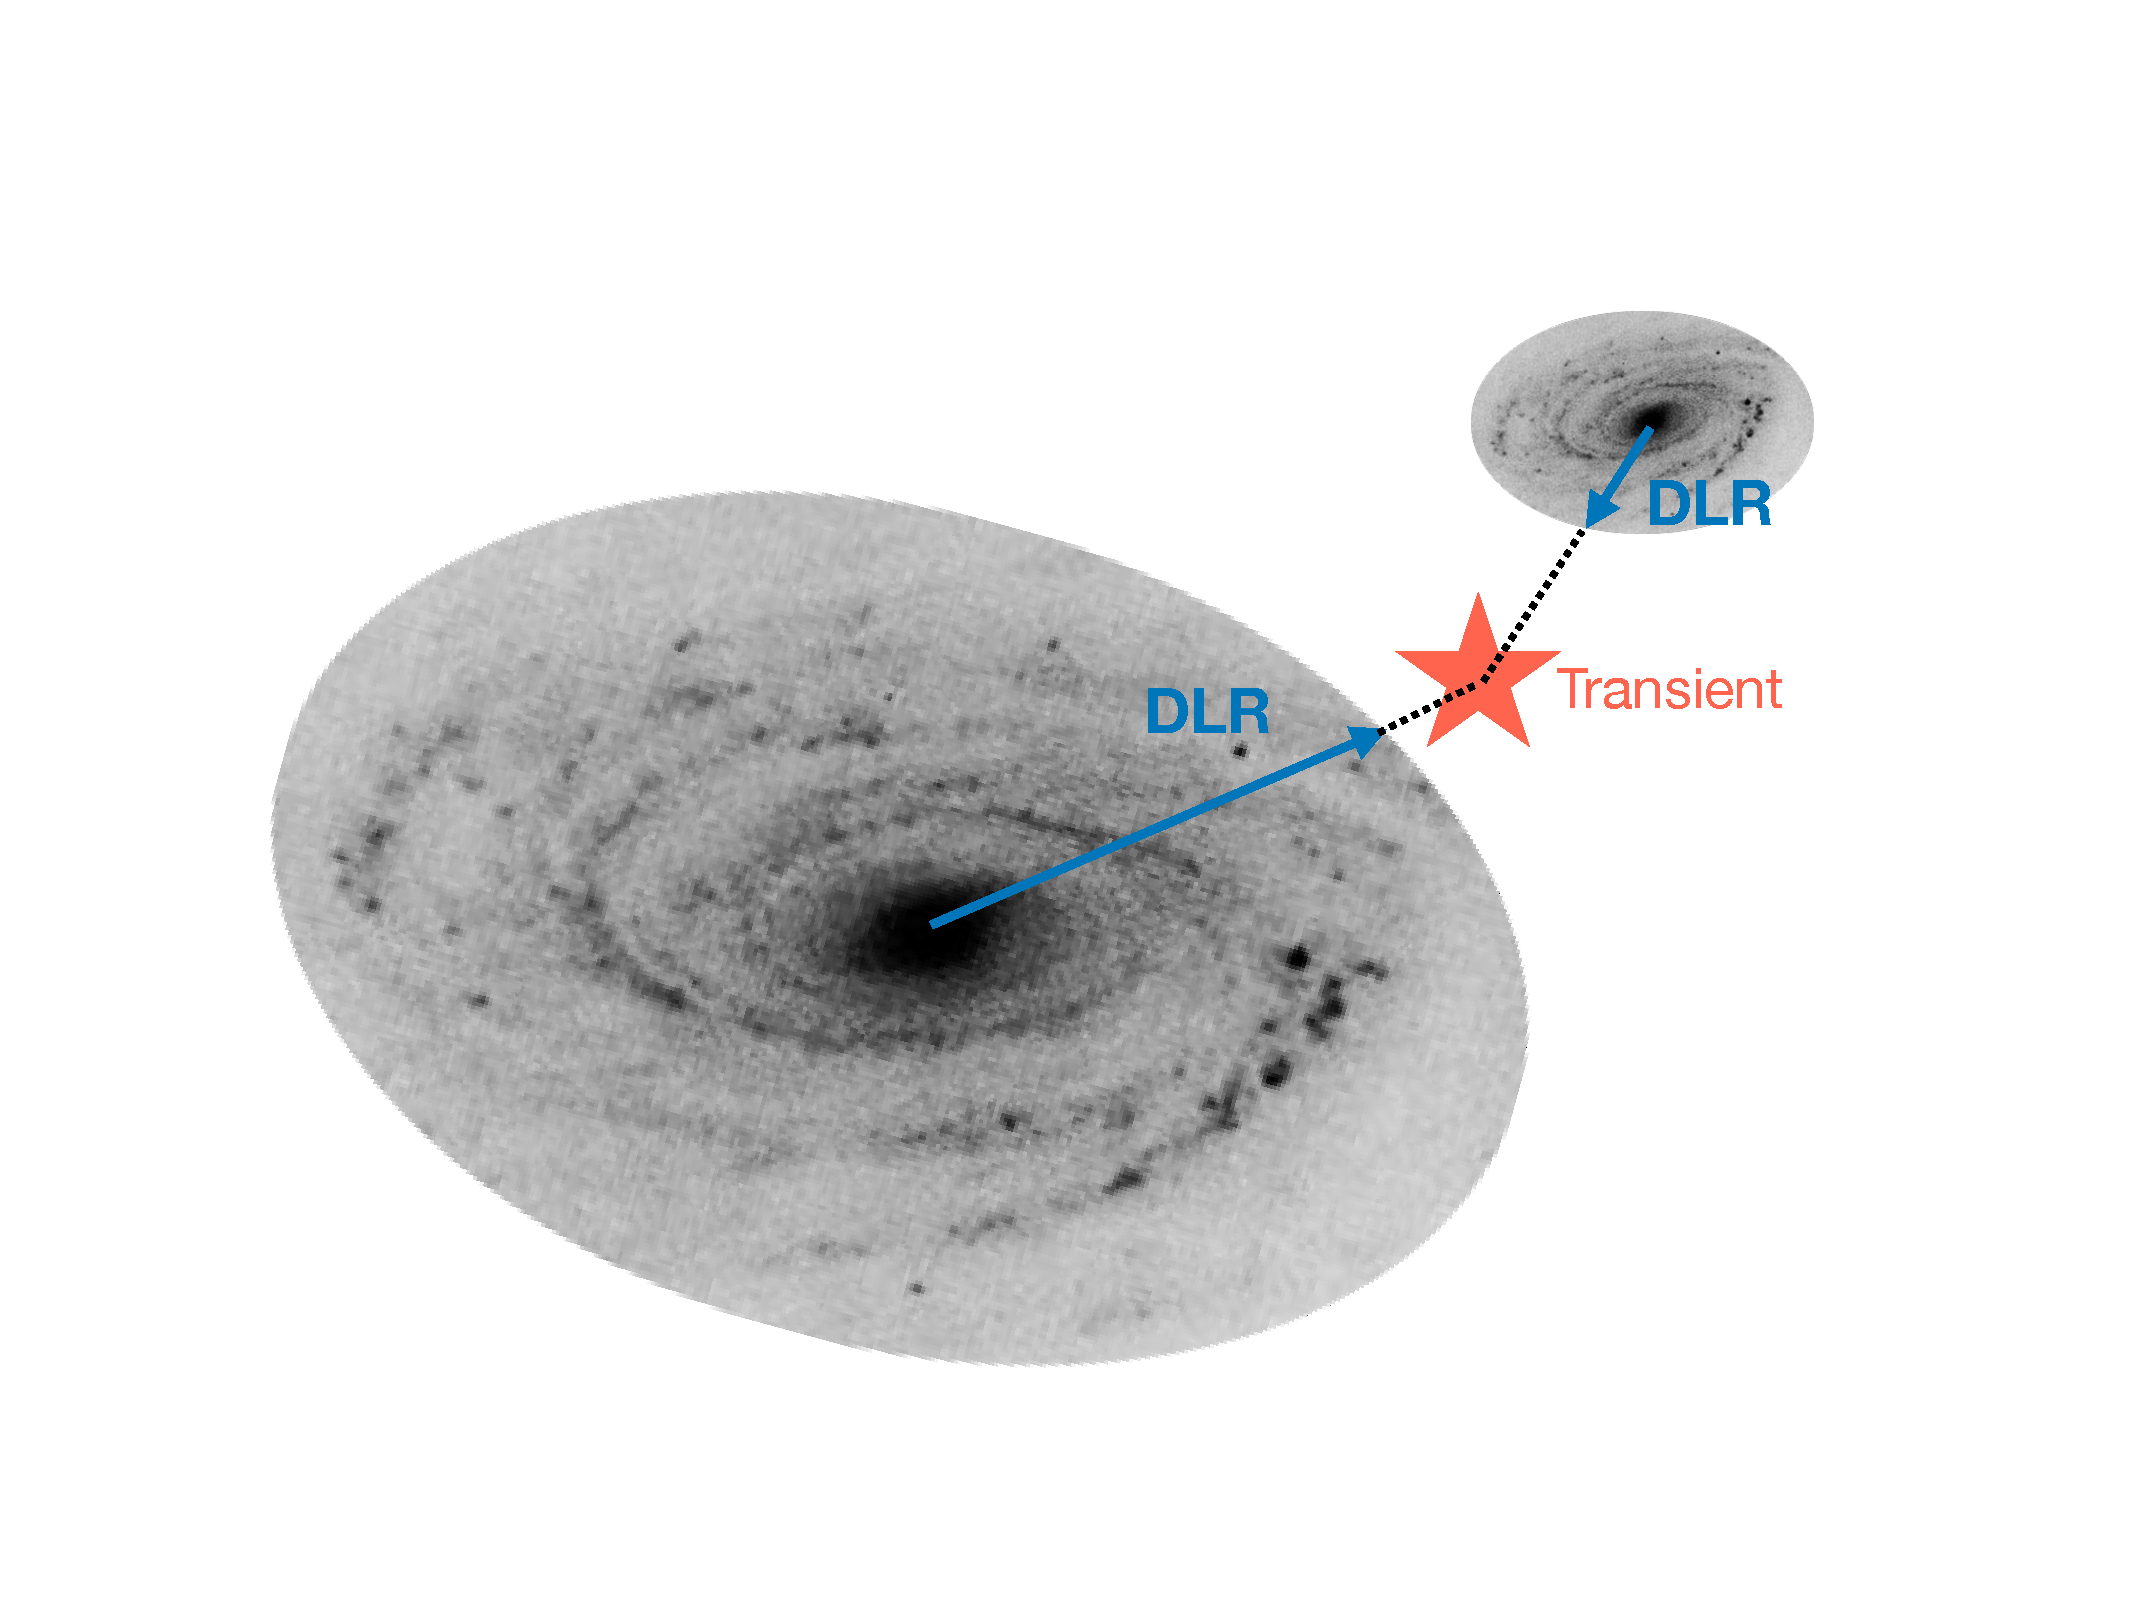
\includegraphics[width=0.6\textwidth]{./chapters/chapter3/Figures/dlr.pdf}
\caption{Illustration of the host matching classification for the transients to different galaxies. In this case, the tranients lies closer to the centre of the smaller galaxy, but the DLR (the directional light radius, shown by the arrows) of the bigger galaxy is larger and its $d_{\rm DLR}$ will be smaller.}\label{fig:DLR}\end{figure}

\subsubsection{SN rejection and host matching}
The light curve (i.e. the flux as a function of time) of a SN may look similar to a closer kilonova, given that the latter is meant to be redder and dimmer than the former. One plausible way of rejecting supernovae in a kilonova search consists in requiring that the observed flux of candidates has significantly declined within 
the first weeks from the trigger (e.g. \citealt{marcelle16} require $S/N<3$ at 24 days), given their longer lightcurve lifetime. This cut will not exclude all the SN, especially those that exploded prior to the trigger. Assuming that those SN happen in galaxies, we identify those contaminant transients by matching them to galaxies, and associating the host galaxy redshift to the SN. If the SN results to be too far to be detected by the GW experiment, we identify it as a SN reject it as a contaminant. This is achieved by constructing a dedicated galaxy catalog with redshifts and morphological information over the whole DECam observable sky (i.e. the whole southern sky up to a declination of 30 deg) and defining a host matching method. 
In our catalog we include galaxies out to redshift $z<0.4$, as that is the furthest distance we would be able to see a SN given the DES-GW strategy for 90 second exposures and a typical $i-$band absolute magnitude at the peak of the SN lightcurve of $-19$.
Host galaxies are searched for in a catalog containing Y3Q2 DES data with \textsc{LePhare} photo$z$-s that I have computed using \texttt{MAG\_AUTO} magnitudes and errors. These galaxies are complemented with 2MASS and SDSS galaxies available in the southern sky. Our host matching script queries the relevant DES Easyaccess database table to obtain transient coordinates which are then matched to potential host galaxies. 
The search is done for each candidate in the HEALPix\footnote{\url{http://healpix.sourceforge.net}} pixel at its position and all the 8 adjacent pixels. Our matching script searches within a 15 arcsec radius from the transient position and ranks all sources according to their dimensionless separation from the transient $d_{\rm DLR}$, which is in units of directional light radius (DLR):
\begin{equation}
d_{\rm DLR}= \frac{\rm galaxy-transient \; angular \; separation\; (arcsec)}{\rm DLR \;(arcsec)}\, ,
\end{equation}
where the DLR is the elliptical radius of a galaxy in the direction of the SN in units of arcseconds. The DLR is computed from some basic morphological quantities from SExtractor: \texttt{A\_IMAGE}, \texttt{B\_IMAGE} and \texttt{THETA\_IMAGE} . These are respectively, the profile RMS along the major and minor axis, and the position angle of the major axis. 
%
%    # convert from IMAGE units (pixels) to WORLD (arcsec^2)
%    A_ARCSEC = A_IMAGE*pix_arcsec
%    B_ARCSEC = B_IMAGE*pix_arcsec
%
%    # angle between RA-axis and SN-host vector
%    GAMMA = np.arctan((DEC_SN - DEC)/(np.cos(DEC_SN*rad)*(RA_SN - RA)))
 %   # angle between semi-major axis of host and SN-host vector
 %   PHI = THETA_IMAGE + GAMMA # angle between semi-major axis of host and SN-host vector
 %   rPHI = A_ARCSEC*B_ARCSEC/np.sqrt((A_ARCSEC*np.sin(PHI))**2 + (B_ARCSEC*np.cos(PHI))**2)

 %   # directional light radius
 %   #  where 2nd moments are bad, set d_DLR = 99.99
 %   d_DLR = angsep/rPHI
This method has already been used for SN searches in by \citet{gupta}. In Figure \ref{fig:DLR}, the DLR for each galaxy is represented by the blue arrows. The maximum value allowed for the $d_{\rm DLR}$ is 4, if no galaxy meets these requirements the candidate is flagged as hostless. If one or more galaxies satisfy this condition, they are assigned a \texttt{DLR\_RANK} depending on their $d_{\rm DLR}$: the lowest $d_{\rm DLR}$ gets a rank of one, and so on up to rank 3, galaxies that are further than the third are excluded. The results are output to a text file and written to the DES database SNGALS table. 

At present we have not put any cut at low redshift for the SN host matching catalog, and therefore matches output from the same code can be used to match potential GW counterparts to host galaxies by separating the matches depending on their redshift, and on the maximum redshift at which the counterpart can be as provided by LIGO.

\begin{figure}
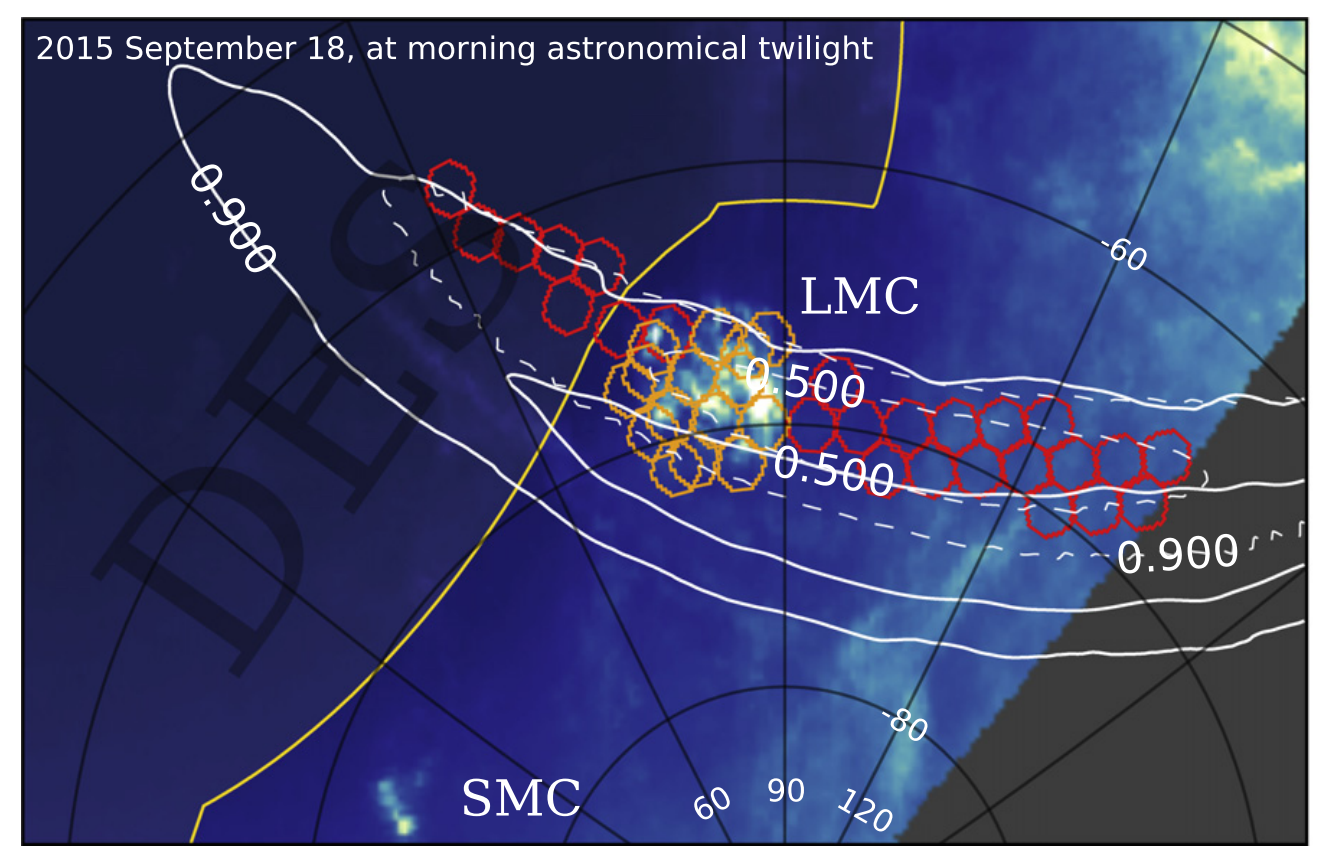
\includegraphics[width=0.52\textwidth]{./chapters/chapter3/Figures/1.png}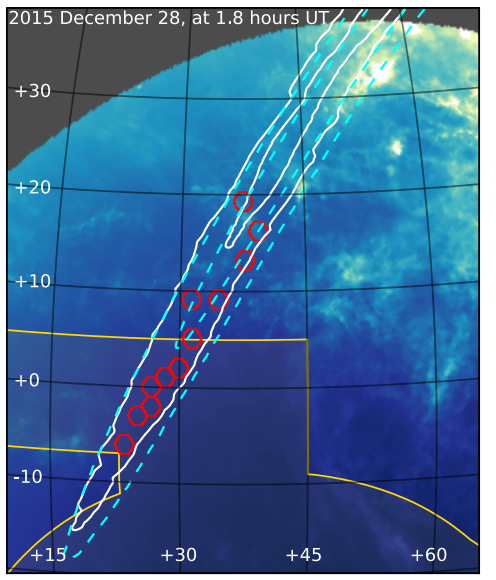
\includegraphics[width=0.29\textwidth]{./chapters/chapter3/Figures/2.png}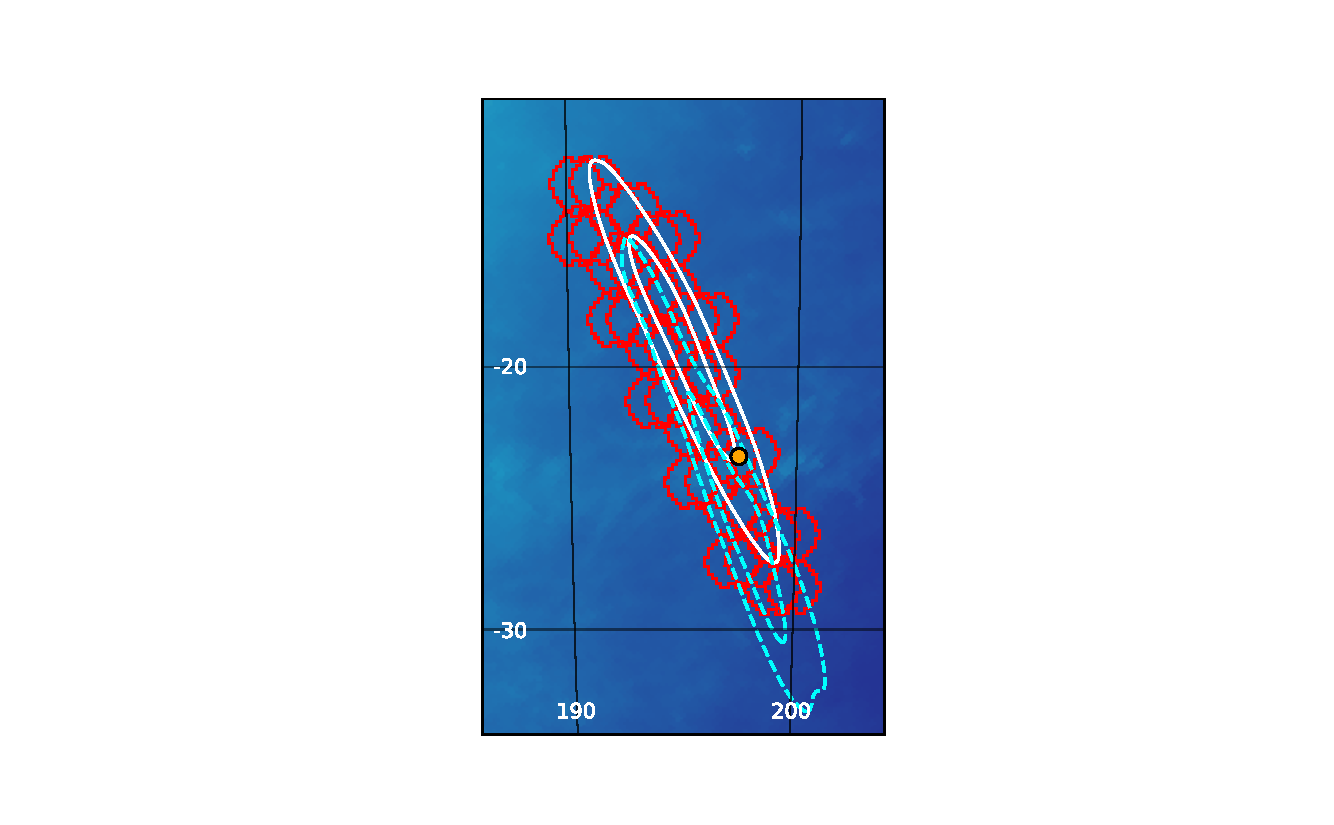
\includegraphics[width=0.22\textwidth]{./chapters/chapter3/Figures/GW170817_skymap.pdf}
\caption{Probability sky map from LIGO containing 90 and 50\% of the probability for the EM counterpart location (solid lines for the updates version, dashed for the first skymap) for GW150914 (left), GW151226 (middle) and GW170817 (right). Red hexagons are the DECam pointings taken as part of the follow--up program. The yellow point in the right hand side panel indicates the position of the kilonova. From \citet{marcelle16}, \citet{Cowperthwaite16} and \citet{marcelle17} respectively.}\label{fig:skymaps}\end{figure}

\subsection{Results from past observing seasons}
During the first LIGO observing season we followed up the two BBH events GW150914 (\citealt{marcelle16}; \citealt{annis16}) and GW151226 (\citealt{Cowperthwaite16}). Neither of the searches found a credible EM counterpart, as all candidates were rejected as background. This result is not surprising, given that (1) we do not expect an EM counterpart to BBH mergers and (2) the observed area was relatively small ($11\%$ and $3\%$ of the LIGO BAYESTAR updated probability map). The large $90\%$ probability region is clear in Figure \ref{fig:skymaps}. During the second observing run, joint detections from LIGO and Virgo were able to reduce these regions by roughly one order of magnitude, from thousands/hundreds of  sq. deg. to hundreds or tens. O2 was a lot more fortunate for the DECam-GW program: we were able to follow up two golden events triggered within 3 days, GW170814 and GW170817, both having 90\% probability regions fully within the DECam observable sky. GW170817 was followed up with enthusiasm, as you will read in the next Section.

\section{GW170817}
The follow up of GW170817 was surely part of the most intense and ambitious programs done in modern astronomy, involving dozens of collaborations all over the world.
On August 17 2017 a GCN (Gamma--ray Coordinate Network) was sent by the \emph{Fermi}-GBM about the detection of a short GRB (sGRB), GRB 170817A, at 12:41:06 UTC. Only 6 minutes after the announcement was sent out, LIGO identified a GW signal that occurred $\sim 1.7$ s before the sGRB. The combination of the data received from the three detectors restricted the sky localisation to 28 ${\rm deg}^2$, and the estimated distance of the event was $\sim 40$ Mpc.
This signal was consistent with that of a BNS coalescence for the first time. In particular, the observed chirp mass was $\mathcal{M}=1.188^{+0.004}_{-0.002} M_\odot$, with a total mass of the system between 2.73 and 3.29 $M_\odot$ and individual masses between 0.86 and 2.26 $M_\odot$. This further supports the BNS scenario against the BBH one, as BHs in BBH systems are usually found to have significantly higher masses. The scenario of a BH-NS binary cannot be ruled out, but the fact that the estimated masses are similar to realistic BNS systems supports the initial BNS hypothesis. 
The follow up included observations in the radio and microwaves (\citealt{Hallinan+17,Alexander+17}), infrared (\citealt{Chornock+17,Kasliwal+17}), optical/UV (\citealt{Arcavi+17,Cowperthwaite,Evans+17,Kilpatrick+17,Lipunov+17,McCully+17,Pian+17,Smartt+17,Shappee+17,marcelle17,Tanvir+17}), X-ray \citep{Troja+17,Margutti+17,Haggard+17,Fong+17},  gamma-ray (e.g.~\citealt{Goldstein+17,Savchenko+17,LIGO+Fermi}), and neutrinos (\citealt{NEUTRINOS}).

GW170817 was followed up extensively by our DECam team, and we imaged $70~{\rm deg}^2$ in $i$ and $z$ band, corresponding to $80.7\%$ of the final probability map. A bright optical transient was detected in our images at 11.4 hours after the GW trigger, and we found it located at $10.6''$ from the centre of NGC 4993 at redshift $z = 0.0098$. This redshift is consistent with the distance of $40\pm8$ Mpc reported by LIGO, provided that $H_0 = 70 {\rm km s^{-1} Mpc^{-1}}$. The apparent magnitudes of the transient at its first detection were $i\simeq 17.30$ and $z\simeq 17.45$, corresponding to an $i-$band absolute magnitude of $M_i=-15.7$, consistent with what expected from kilonova models. After performing the difference imaging, we found $1,500$ potential transient candidates, all but one rejected as background sources after some simple selection cuts, which include rejecting SN events. Thus the candidate found in NGC 4993 is the only plausible GW counterpart, and we reject chance of coincidence at the $99.5\%$ confidence level. Our analysis of the GW170814 follow up images is on--going and still blinded. However, we find that our method for SN rejection through galaxy matching allows us to exclude $\sim 50\%$ of candidates with a machine learning score of $\geq 0.7$. This method has been tested on SN events simulated with \textsc{SNANA} (\citealt{snana}).


%%%%%%%%%%%%%%

\section{GW170817 Host galaxy follow up with DECam}\label{sec:gw170817}

\begin{figure}
\centering
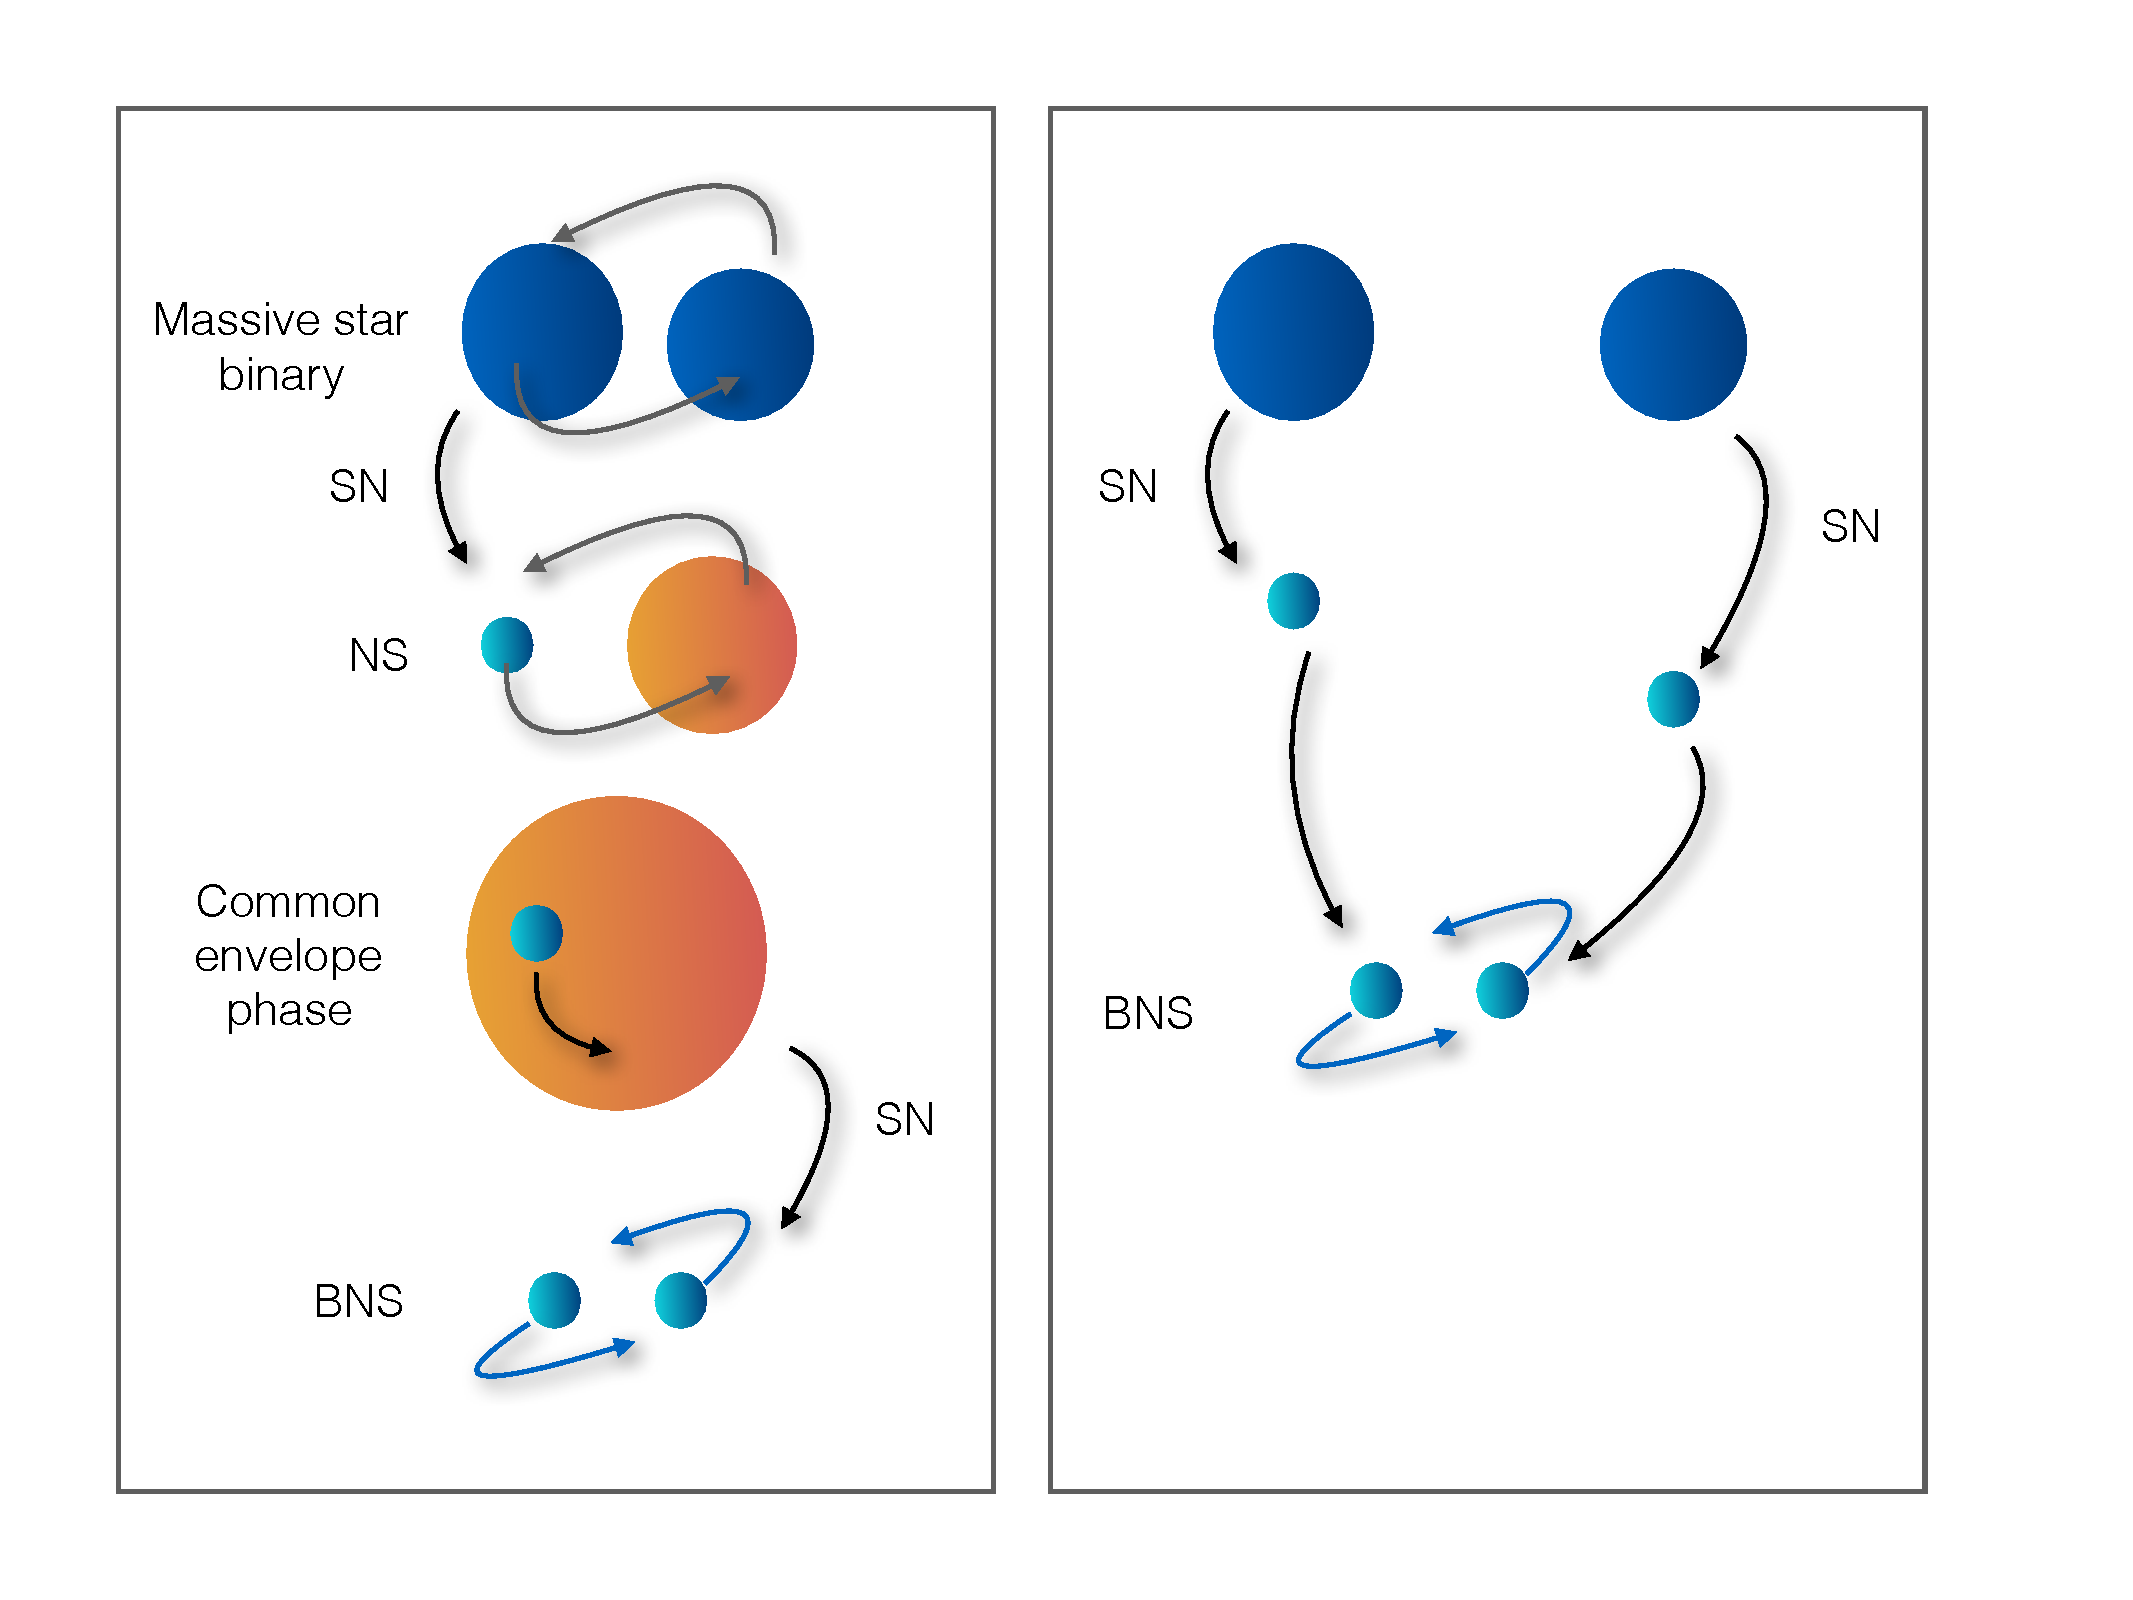
\includegraphics[width=0.6\textwidth]{./chapters/chapter3/Figures/diagram.pdf}
\caption{Possible formation channels for binary neutron stars. \emph{Left:} pure or secular star formation scenario. The binary is formed as a system during some star formation event, and follows the usual steps of stellar evolution: the most massive of the two stars undergoes a supernova event and becomes a neutron star.}\label{formationfig}\end{figure}

While the models predicting optical and NIR emission from the coalescence of binary neutron stars are widely accepted in the astronomical community, the formation of the binary and the physics involved in merging are still a matter of debate (\citealt{bns}; \citealt{bns2}). In this work we use this DECam data and supplement it with Hubble Space Telescope, AAT spectroscopic data and with publicly available datasets to understand the source of GW170817 in the context of its host galaxy and the local environment. In particular, we relate the BNS formation to the dynamics and stellar evolution of the host over time, asking whether the binary system was born as such, or whether dynamical interactions caused its formation. Usually it is assumed that BNSs form through the scenario that we call ``pure star formation''. In this case, the binary of two massive stars is formed as a system during some star formation event, and follows the usual steps of stellar evolution: the most massive of the two stars undergoes a supernova event and becomes a neutron star, and before the second star also undergoes a SN explosion, there is a ``common envelope phase'' in which the NS is orbiting in the outer layers of the other star. Once the second star also becomes a NS, if the binary is still bound after the two explosions, and it is close enough to merge within a Hubble time, then this system will be a source of GW emission at merging that we can observe.

Dynamically--driven binary formation has been proposed for BBH (e.g. \citealt{bbh1}). By dynamically--driven, we mean any dynamical interaction that may facilitate the formation of a BNS that can merge in less than a Hubble time. In the simplest case, two single NS may form a binary system due to a close encounter. Given the typical dimensions of NS, their cross sections are not large and this is only a possibility in very dense stellar environments. Other dynamical processes may intervene: a widely separated binary system may be brought to a orbit on a shorter distance due to interactions with a third body, or an existing binary system including one NS may capture another NS. See Figure \ref{formationfig} for a schematic representation of the two different scenarios presented.

Previous studies (\citealt{1988MNRAS.235..813C}) classified this galaxy as an atypical elliptical galaxy with faint concentric shells and spectral features suggesting that the galaxy has undergone a merging event. Several analytical and numerical studies support the galaxy merger scenario for the formation of shells in galaxies (e.g. \citealt{quinn}; \citealt{pop}), and show that the distribution of shells can constrain the time of the merger event. We study the evolution of this galaxy to
discern between different BNS formation scenarios and estimate the rate of BNS formation in early-type galaxies, using Dark Energy Survey (DES) data to place NGC4993 in the context of the galaxy population.

\subsection{Data}\label{datasec}

\subsubsection{Photometric data: DECam, VHS and HST}

\begin{sidewaysfigure}
\centering
\includegraphics[width=1\textwidth]{./chapters/chapter3/Figures/f1.pdf}
\caption{\emph{Left panel:} DECam coadded image of NCG4993 in $gri$. Shell structures indicative of a recent galaxy merger are clearly visible. \emph{Middle panel:} $r$-band residuals from \galfit after subtraction of the best-fit single S\'ersic light profile. \emph{Right panel:} F606W-band HST ACS image with a 3 component galaxy model subtracted. Dust lanes crossing the centre of the galaxy are evident. The green lines show the position of the transient. The BNS counterpart is only present in the middle panel.
}\label{coaddimage}\end{sidewaysfigure}

The DECam images used in this work were taken as part of the DECam-GW follow up program between the nights of 2017 August 17 and September 1, using $ugrizY$ filters. We also use public $ugrizY$ DECam data from June 2015 to avoid contamination in the transient region. In addition, we extract $YJK$ data from the VISTA Hemisphere Survey (VHS; \citealt{vista}), covering the host galaxy.
The images are coadded and registered to a common pixel scale ($0.2636''$) using \texttt{SWARP} \citep{swarpref} with $3.5$ sigma clipping to remove cosmic ray artifacts. An RGB coadded image of the galaxy is presented in Figure \ref{coaddimage}. We build a $\chi^2$ detection image from the $r$, $i$ and $z$-band data and run \sextractor \citep{sextractor} in dual mode on the coadded images. 

The photometry is corrected for galactic extinction. 
In order to compare the galaxy properties to a broader sample, we also use DES data from the first year of observations (Y1; \citealt{firstyear}).
We use \texttt{MAG\_AUTO} magnitudes unless otherwise stated.

NGC4993 was also observed during HST Cycle 24
(PropID 14840, PI: Bellini) using ACS in F606W. The data were publicly released in April 2017 and were accessed via the Hubble Source Catalog (HSC;  \citealt{whitemore}).

\subsubsection{Spectroscopic data: 6dF and AAT}

The 6dF Galaxy Survey (\citealt{6dfgs}) final release (\citealt{6df}) includes an optical spectrum of the center of NGC4993 with an estimated redshift ($z=0.009680 \pm 0.000150$). 

Spectra of 14 galaxies with $v_{helio}\sim3000~{\rm km}~{\rm s}^{-1}$ and within one degree radius of NGC4993 were obtained in one target of opportunity exposure of the AAOmega spectrograph at the Anglo--Australian Telescope (AAT) on 2017 August 27. Of those, 10 spectral fits passed quality cuts.
All the spectra used here are centered on their galaxy nucleus with a $2''$ aperture.


%%%%%%%%%%%%%%%%%

\subsection{Host morphology}\label{morphsec}

\subsubsection{CAS and Galfit}\label{paramfitting}

We begin our study of NGC4993 with an analysis of its morphological properties, employing the $CAS$ non-parameteric light quantification \citep{conselice} and parametric S\'ersic light profile fitting with \textsc{GalFit} \citep{Peng}. Both methods utilise a mask to exclude other sources in the image and the location of the kilonova event. The $CAS$ system is able to pick out the salient features of galaxy morphology, allowing galaxy types to be assigned and identifying objects that are likely to have undergone a recent major merger. Meanwhile, fitting the light profile additionally provides us with an alternative estimate of the total magnitude and can reveal more subtle aspects of galaxy morphology within the residuals of the model-subtracted image.

The $CAS$ system estimates three morphological parameters, concentration $C$, asymmetry $A$, and clumpiness $S$ to classify objects. The concentration is defined as the logarithm of the ratio of the $80\%$ to 20\% curve of growth radii $r_{80}, r_{20}$:
\begin{equation}
C=5\times \log_{10}(r_{80}/r_{20})\,,
\end{equation}
where the curve of growth is the integrated flux inside an aperture of radius $r$ as a function of $r$.
In general, elliptical galaxies tend to be more concentrated than disk galaxies and dwarf galaxies. In order to compute the asymmetry $A$ we rotate the galaxy image $I$ by $180^o$ ($R$) and subtract it from its original image. The absolute value of these residuals is divided by the original image flux $I$, so that: $A=|I-R|/I$. The asymmetry is particularly related to the merger history. The clumpiness $S$ is given by subtracting the original image of the galaxy by a smoothed image, so that the residual map only contains the high-frequency components of the light distribution:
\begin{equation}
S=10 \times \Sigma^{N,N}_{x,y=1,1}\frac{(I_{x,y}-I_{x,y^{\sigma}})-B_{x,y}}{I_{x,y}}\,,
\end{equation}
where $I_{x,y}$ is the sky--subtracted galaxy flux in the pixel at $(x,y)$, $I_{x,y}^{\sigma}$ is the map smoothed with a filter of width $\sigma$ and $B_{x,y}$ is the background flux value in an area which is equivalent to that of the galaxy. Elliptical galaxies are usually very smooth and therefore present a low clumpiness value, while star forming galaxies can be very patchy and present a high $S$ value.
The $CAS$ quantities are all defined within 1.5 times the Petrosian inverted radius at $r(\eta=0.2)$, where $\eta$ is a dimensionless quantity defined in terms of the surface brightness at radius $r$: $\eta\equiv I(r)/\langle I(r)\rangle$\footnote{This is the inverse of the definition that was introduced by \citet{petrosian}}. This radius was chosen because more than 99\% of the light is included within $r(\eta= 0.2)$. For a detailed definition and analysis of these parameters see \citet{Bershady}.

\textsc{GalFit} is run on the DES and VHS images to fit the galaxy with a Single Sersic profile, performing the deconvolution with a PSF model extracted with \textsc{PSFEx} \citep{psfex} and using input guesses from \sextractor. As reported in  \citep{Peng}, the adopted S\'ersic function has the following form: 
\begin{equation}
\Sigma(r) = \Sigma_e \exp{ \bigg[ -k \bigg(\frac{r}{r_e}\bigg)^{\frac{1}{n}} -1 \bigg]} ,
\label{eq:sersicfunction}
\end{equation}
where $\Sigma_e$ is the pixel magnitude at the effective radius $r_e$. The S\'ersic index \textit{n} quantifies the profile concentration: if \textit{n} is large, we have steep inner profile with a highly extended outer wing;  inversely, when \textit{n} is small, the inner profile is shallow and presents a steep truncation at large radii. In the case of $n=1$ we have an exponential light profile, while for $n=4$ it reduces to a de Vaucouleurs profile.
\textsc{Galfit} provides measurements for the free parameters of the S\'ersic function: central position, integrated magnitude $m_{\rm tot}$, effective radius $r_e$ measured along the major axis, S\'ersic index $n$, axis ratio $q$ and position angle $\theta$. The integrated magnitude is determined through its definition as a function of the flux integrated out of $r=\infty$ for the S\'ersic profile. %:
%\begin{equation}
%m_{tot} = -2.5 \log_{10}{\bigg(\frac{F_{tot}}{t_{exp}}\bigg)} +m_{\rm ZP},
%\label{eq:integratedmagnitude}
%\end{equation}
%where $t_{exp}$ is the exposure time and $m_{ZP}$ is the magnitude zero point, both indicated in the image header. 
The fit is done in two ways: band-by-band and simultaneously across all bands using a modified version, \textsc{GalFit-m} \citep{galfitm}. In the second case the S\'ersic fitting parameters are allowed to vary with wavelength as a second-order polynomial. %We extract the PSF model required by \textsc{GalFit} from the coadd images with \textsc{PSFEx} \citep{psfex} and initialize the fitting parameters based on measurements of the galaxy from \textsc{sextractor}. 
All parameters are left free without constraints, except for the central position in the single-band fits. This is allowed to vary by only $\pm 1$ pixel as it is well-constrained by \sextractor already.

In order to assess the stability of \textsc{GalFit} and obtain an estimate of the uncertainties on the measurements, each single--band run is performed 10,560 times, varying the inputs around their nominal values. We take the median as our final measurement and the standard deviation as the uncertainty.

\begin{figure}
\centering
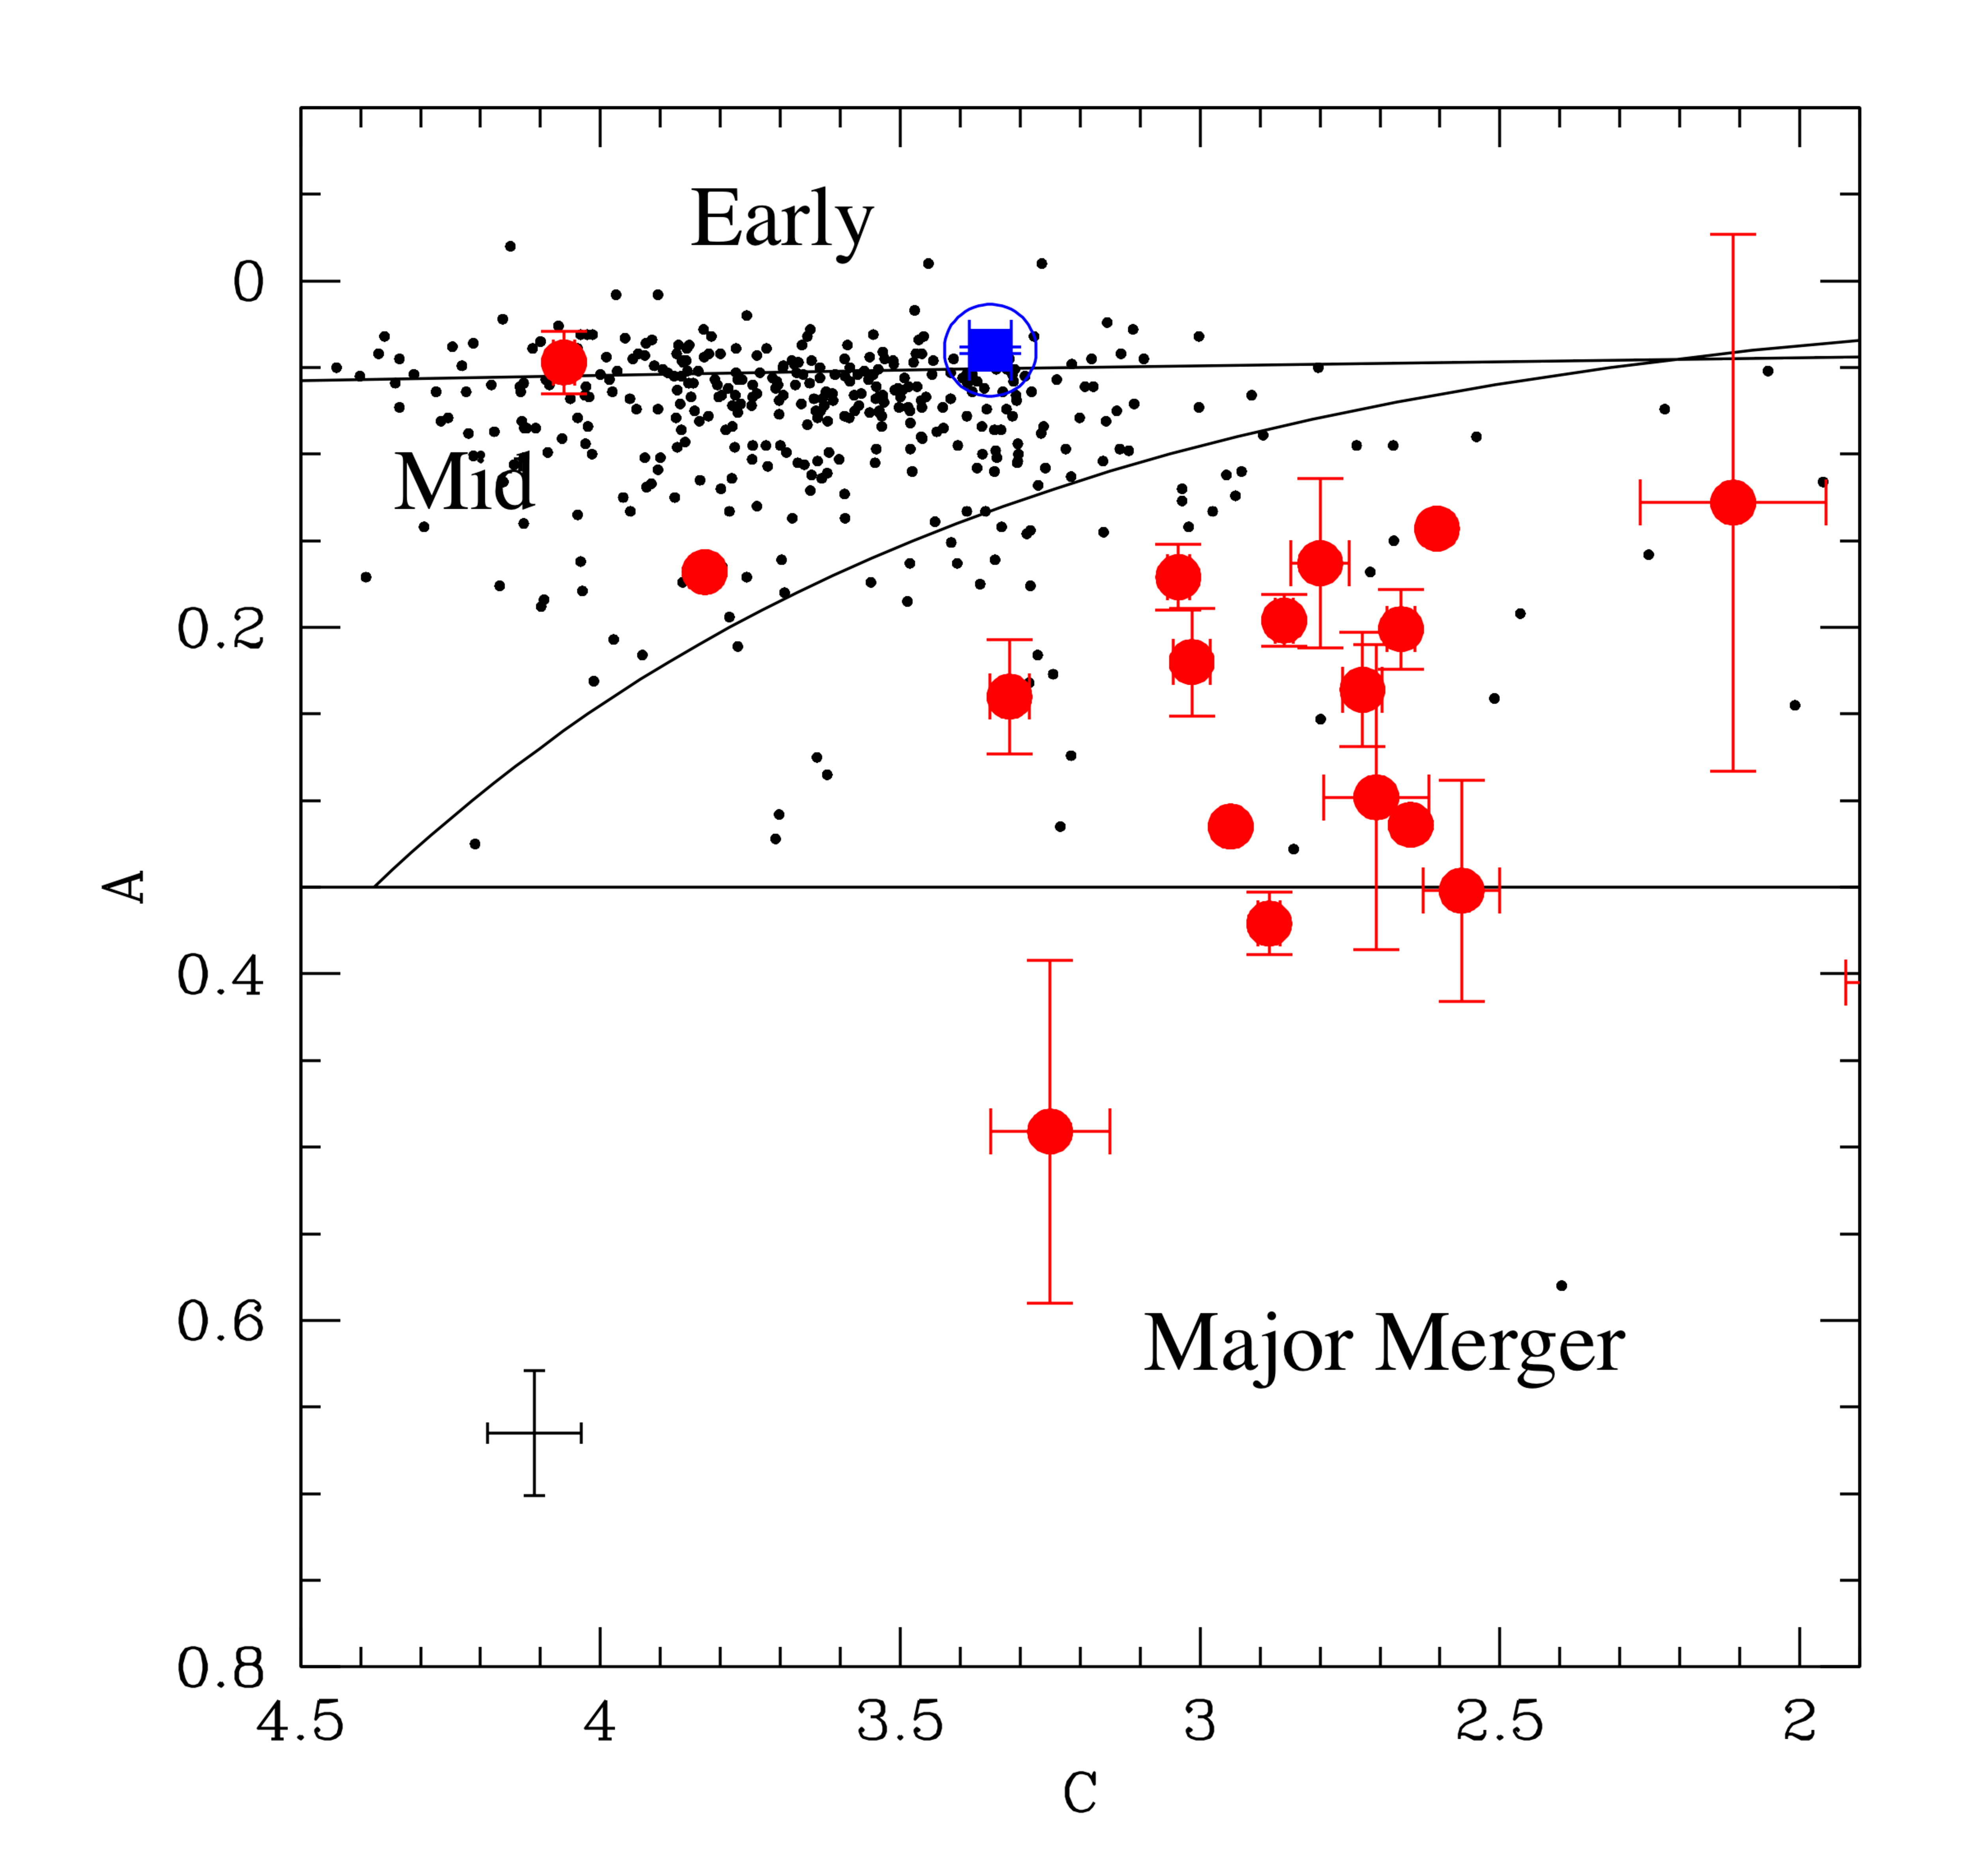
\includegraphics[width=0.7\textwidth]{./chapters/chapter3/Figures/f2.pdf}\caption{Concentration versus asymmetry for NGC4993 (in blue), compared to a sGRB hosts sample (Conseliece et al., in prep.) in red, and field galaxies (black dots) with stellar mass within $\pm 0.2$ dex of NGC4993 value and redshift $z<0.2$. The lines separate different Hubble types as shown in \citet{conselice}.}\label{sgrb}\end{figure}

\begin{table*}
\centering
\begin{tabular}{c|cccccc}
\hline
\hline

Filter & \texttt{MAG\_AUTO} & Mag & $r_e$ & $n$ & $\epsilon$ & $\theta$\\
\hline
$u$ & 14.24 & 14.15 & 61.8 & 3.2 & 0.15 & -13.9\\
$g$ & 12.95 & 12.80 & 62.5 & 3.4 & 0.15 & -12.8\\
$r$ & 12.08 & 11.90 & 63.5 & 3.7 & 0.16 & -11.2\\
$i$ & 11.65 & 11.45 & 64.4 & 4.0 & 0.16 & -9.9\\
$z$ & 11.34 & 11.13 & 65.3 & 4.3 & 0.16 & -8.4\\
$Y$ & 11.13 & 10.96 & 65.7 & 4.4 & 0.16 & -7.7\\
$Y_{{\rm VHS}}$ & 11.27 & 11.00 & 65.9 & 4.5 & 0.16 & -7.5\\
$J$ & 11.00 & 10.77 & 67.3 & 5.0 & 0.17 & -5.2\\
$K_s$ & 11.08 & 10.68 & 72.9 & 6.7 & 0.19 & +3.5\\
\hline
 & & $\pm 5\times10^{-4}$ & $\pm 0.07$ & $\pm 3\times10^{-3}$ & $\pm 4\times10^{-5}$ & $\pm 5\times10^{-3}$ \\
\hline

\end{tabular}\caption{Outputs from \textsc{Galfit} parametric S\'ersic fits performed on the $ugrizY$ DECam coadd images and $YJKs$ VHS data. The fit was joint across bands, allowing the effective radius, $r_e$ (in pixels), S\'ersic index, $n$, ellipticity, $\epsilon=1-b/a$, and position angle, $\theta$, to vary with wavelength. One pixel corresponds to $0.2636''$. The final row lists indicative errors based on the single band analysis.}\label{tablefit}
\end{table*}

\subsubsection{Results}
\label{morphresults}
Following the definitions given in \citet{conselice}, we find: concentration $C=3.348\pm 0.035$, asymmetry $A=0.04\pm 0.01$, and clumpiness $S=0.05\pm 0.05$. These values are typical for an early-type galaxy. In Figure \ref{sgrb} we compare these values to field galaxies of similar masses (within 0.2 dex of NGC4993) and redshifts ($z<0.2$) from the GAMA survey, and to a sample of sGRB hosts (Conselice et al. in prep.) taken in F814W imaging from HST. NGC4993 stands out as peculiar with respect to other GRB hosts: such objects tend to lie on the more highly asymmetric side of late-type galaxies.

The results from the single S\'ersic fit across all bands are summarized in Table \ref{tablefit} (the band-by-band fits give broadly consistent results). We find an increase in S\'ersic index towards redder bands and a rotation in the position angle. 
This rotation of bluer versus redder bands suggests there could be two superimposed stellar populations with differing orientations. This may have arisen during the course of the galaxy's secular evolution but could also be caused by a minor galaxy merger, as indicated by the presence of shells.

The middle panel of Figure \ref{coaddimage} shows DECam $r$-band residuals from \galfit and the position of the transient. At least four shell structures are clearly visible. Closer inspection with HST data (right panel in Figure \ref{coaddimage}) reveals a possible further broad inner shell, on which the transient seems to lie, and obvious dust lanes (visible also as a negative residual in the DECam version).  The $r$-band absolute magnitude from a $4~{\rm sq.arcsec}$ region around the transient location in the galaxy-subtracted template image is $-10.65$. This luminosity implies a rather high stellar density in the locale of the BNS coalescence. In summary, we find compelling evidence for a recent minor galaxy merger in NCG4993, and the location of the kilonova event with respect to the shells leads us naturally to ask whether there is a causal connection between the two.  

From Figure \ref{sgrb} we see that clear major galaxy mergers are unusual amongst sGRB hosts. Furthermore, the other sGRBs are at cosmological distances and thus are mostly undergoing extensive galaxy formation through star formation or merging.  If the hosts have to be related by some common features, this is an indication that NGC4993 has undergone some merging activity, but a minor merger such that the bulk morphology is still elliptical. We thus explore the possibility that the kilonova was a result of a recent galaxy merger in NGC4993.

%%%%%%%%%%%%%%%%%%%%%%

\subsection{Photometric and spectroscopic SED}\label{sedsec}

\begin{figure}
%\hspace{-0.5cm}
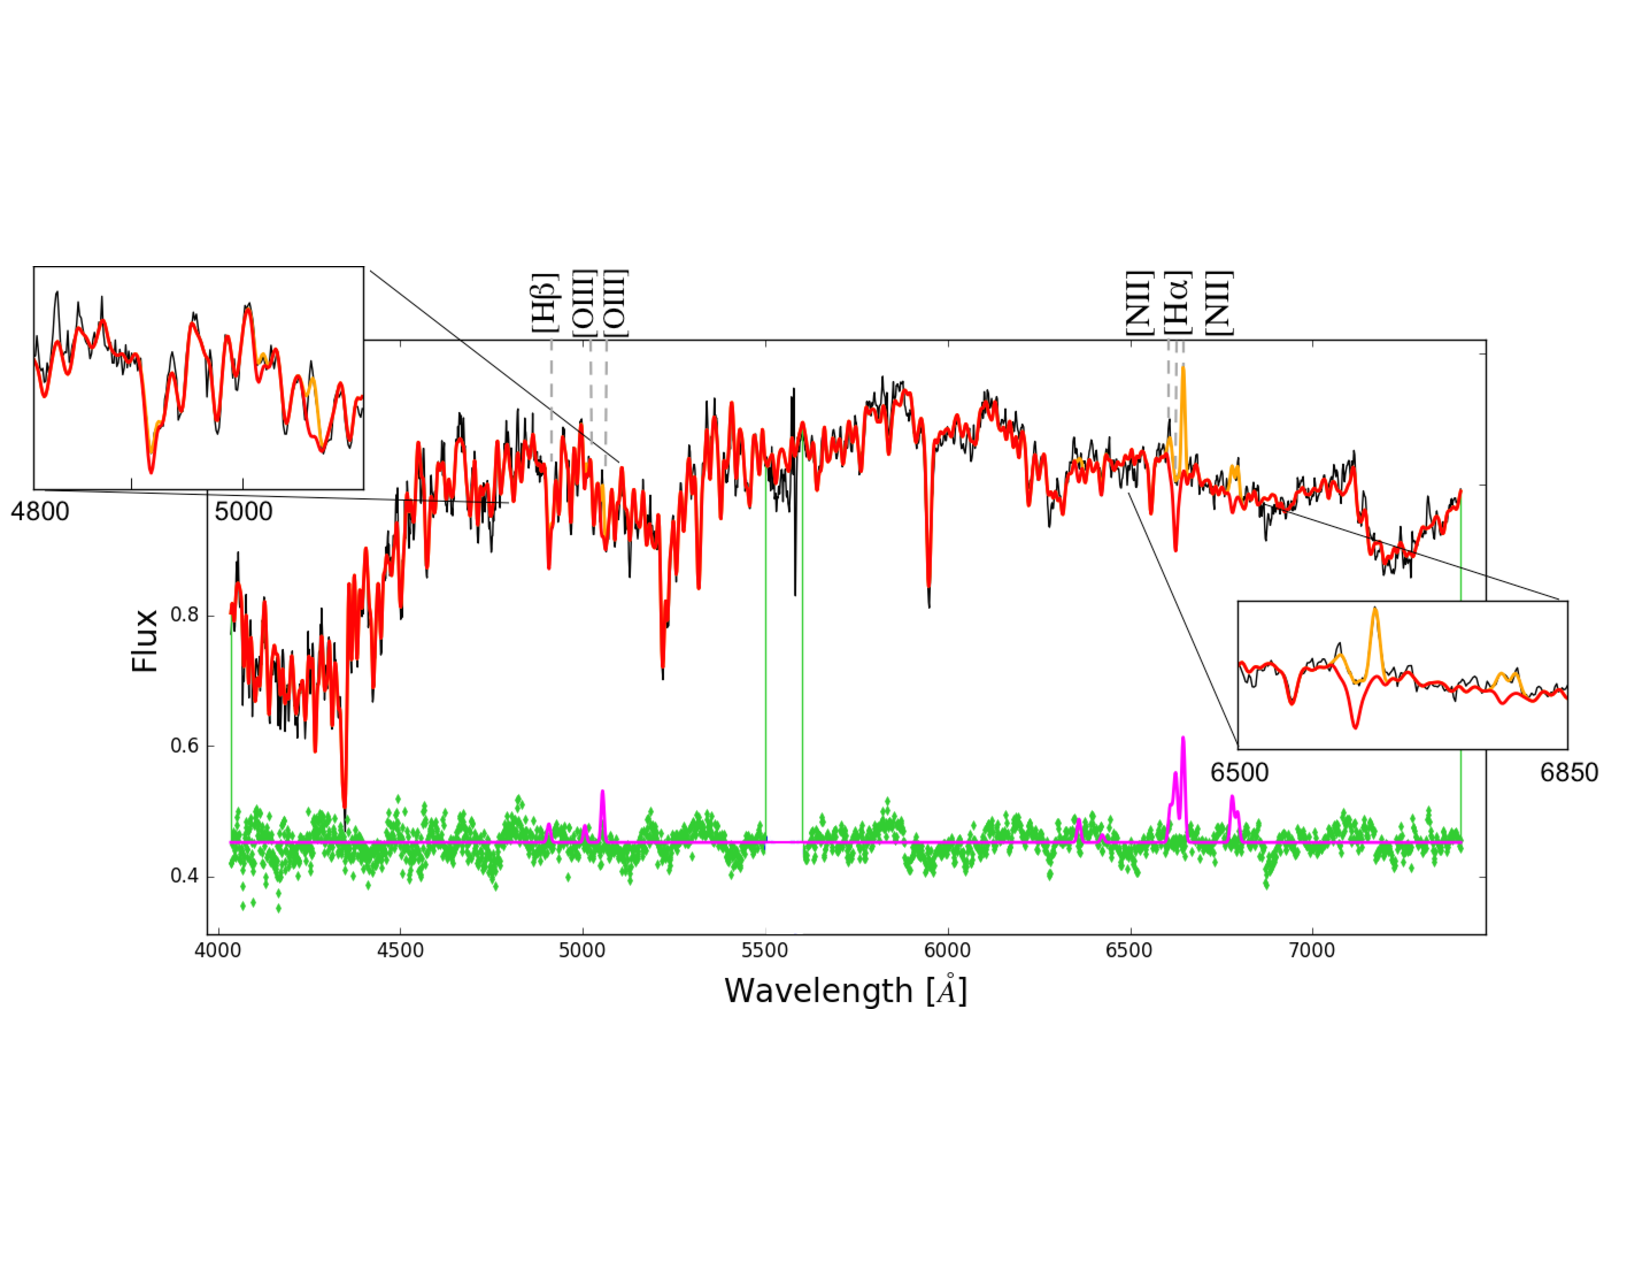
\includegraphics[width=1\textwidth]{./chapters/chapter3/Figures/f3a.pdf}%\hspace{-0.1cm}\vspace{-0.1cm}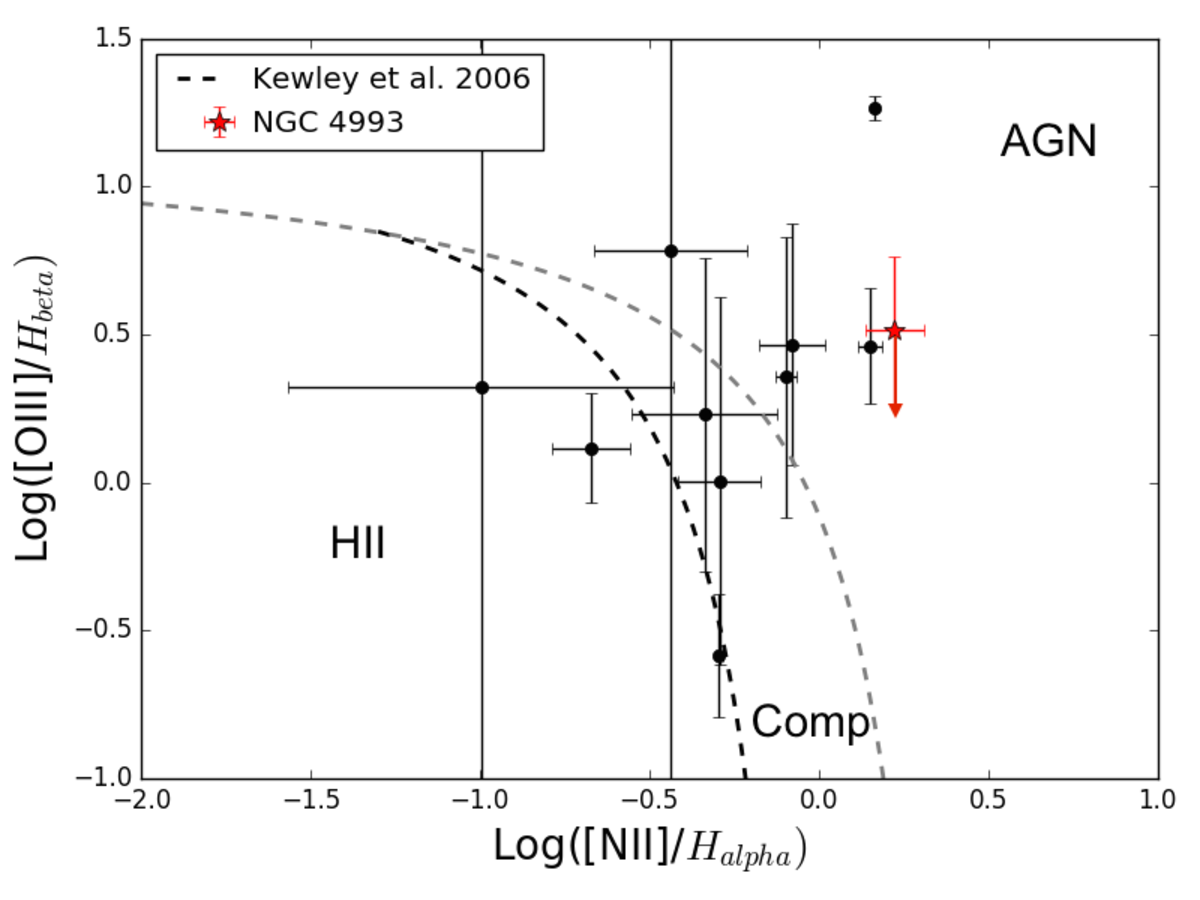
\includegraphics[width=0.4\textwidth]{./chapters/chapter3/Figures/f3b.pdf}
\caption{Spectroscopic fit of the 6dF optical spectrum. The black line is the observed spectrum,the red line is the \textsc{pPXF} fit for the stellar component, and the orange line is the best--fit including ionized gas emission lines. The zoomed panels show $H_\beta$, OIII, NII and $H_\alpha$ lines. The green points at the bottom are the fit residuals, while the purple line is the gas-only best--fit model spectrum. }\label{spec}\end{figure}

\begin{figure}
%\hspace{-0.5cm}
\centering
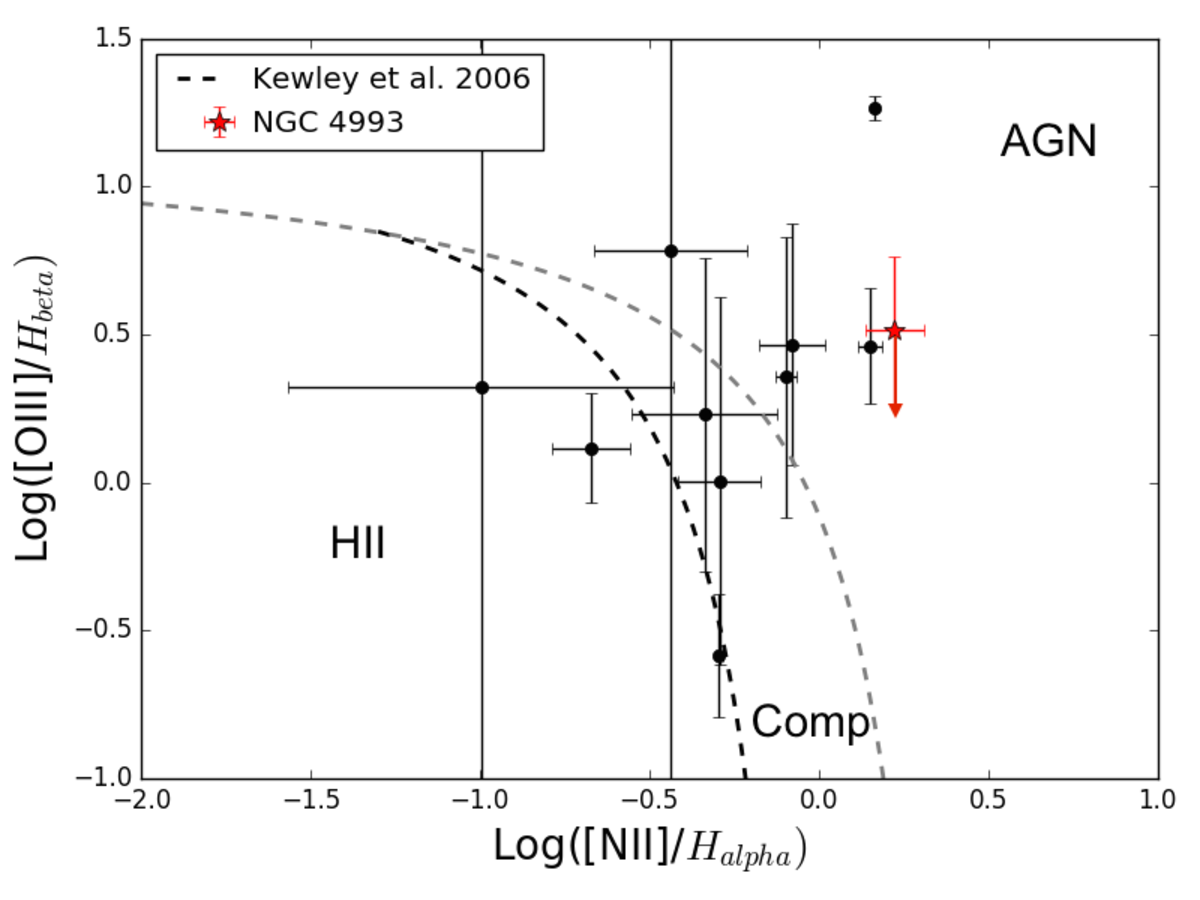
\includegraphics[width=0.6\textwidth]{./chapters/chapter3/Figures/f3b.pdf}
\caption{BPT diagram for NGC4993 (red star) and the other galaxies (black points) in the galaxy group with AAT spectra available. The dashed lines represent the \citet{2006MNRAS.372..961K} classification method for AGN, star--forming (HII) and composite (Comp) galaxies. Many of the group galaxies have very weak AGN or LINER-like emission. Error bars represent 1$\sigma$ error from the propagation of fit errors on line strengths.}\label{fig:bpt}\end{figure}


\subsubsection{SED fitting methods}
We use \ppxf (\citealt{ppxf}; \citealt{ppxf1}), for the spectral fitting. It enables extraction of the stellar kinematics and stellar population from absorption line spectra of galaxies, using a maximum penalized likelihood approach. We use the Miles stellar libraries, and fit over the wavelengths $4000-7409 $ \AA, excluding the range $5500-5600$ \AA\, of the 6dF spectrum, where a strong sky line contaminates the flux.

We use \lephare (\citealt{arnouts}, \citealt{ilbertlephare}) for the broadband Spectral Energy Distribution (SED) fitting. 
We add a 0.05 systematic uncertainty in quadrature to the magnitudes. 
The simple stellar population (SSP) templates used are \citet{bc03}, with two metallicities ($Z_\odot$ and $2.5Z_\odot$), a \citet{chabrier} Initial Mass Function (IMF) and a Milky Way \citep{allen} extinction law. The SFH chosen is lognormal:
\begin{equation}
  \Psi(t,t_0,\tau)=\frac{1}{t\sqrt{2\pi\tau^2}}e^{-\frac{(\ln t-\ln t_0)^2}{2\tau^2}}\,,  \label{sfr} 
\end{equation}
as it is the most representative family of models with only two parameters \citep{lognorm}. Here $t_0$ and $\tau$ are the half--mass--time and width.

Motivated by our morphological analysis, we allow for an additional burst of recent SF. This is modeled as a Gaussian centered at $t_{burst}$ with width of 10 Myr and peaking at a fraction $0.4-0.1$ of the peak of the log-normal SFH (as no evidence for strong late SF is found).

The same templates are used to perform spatially--resolved SED fitting across DES+VHS coadded images within $10\times10$ pixels, including the galaxy dust extinction. The other sources in the field are masked out using the segmentation map output by \textsc{sextractor}.

\begin{figure}
%\hspace{0.6cm}
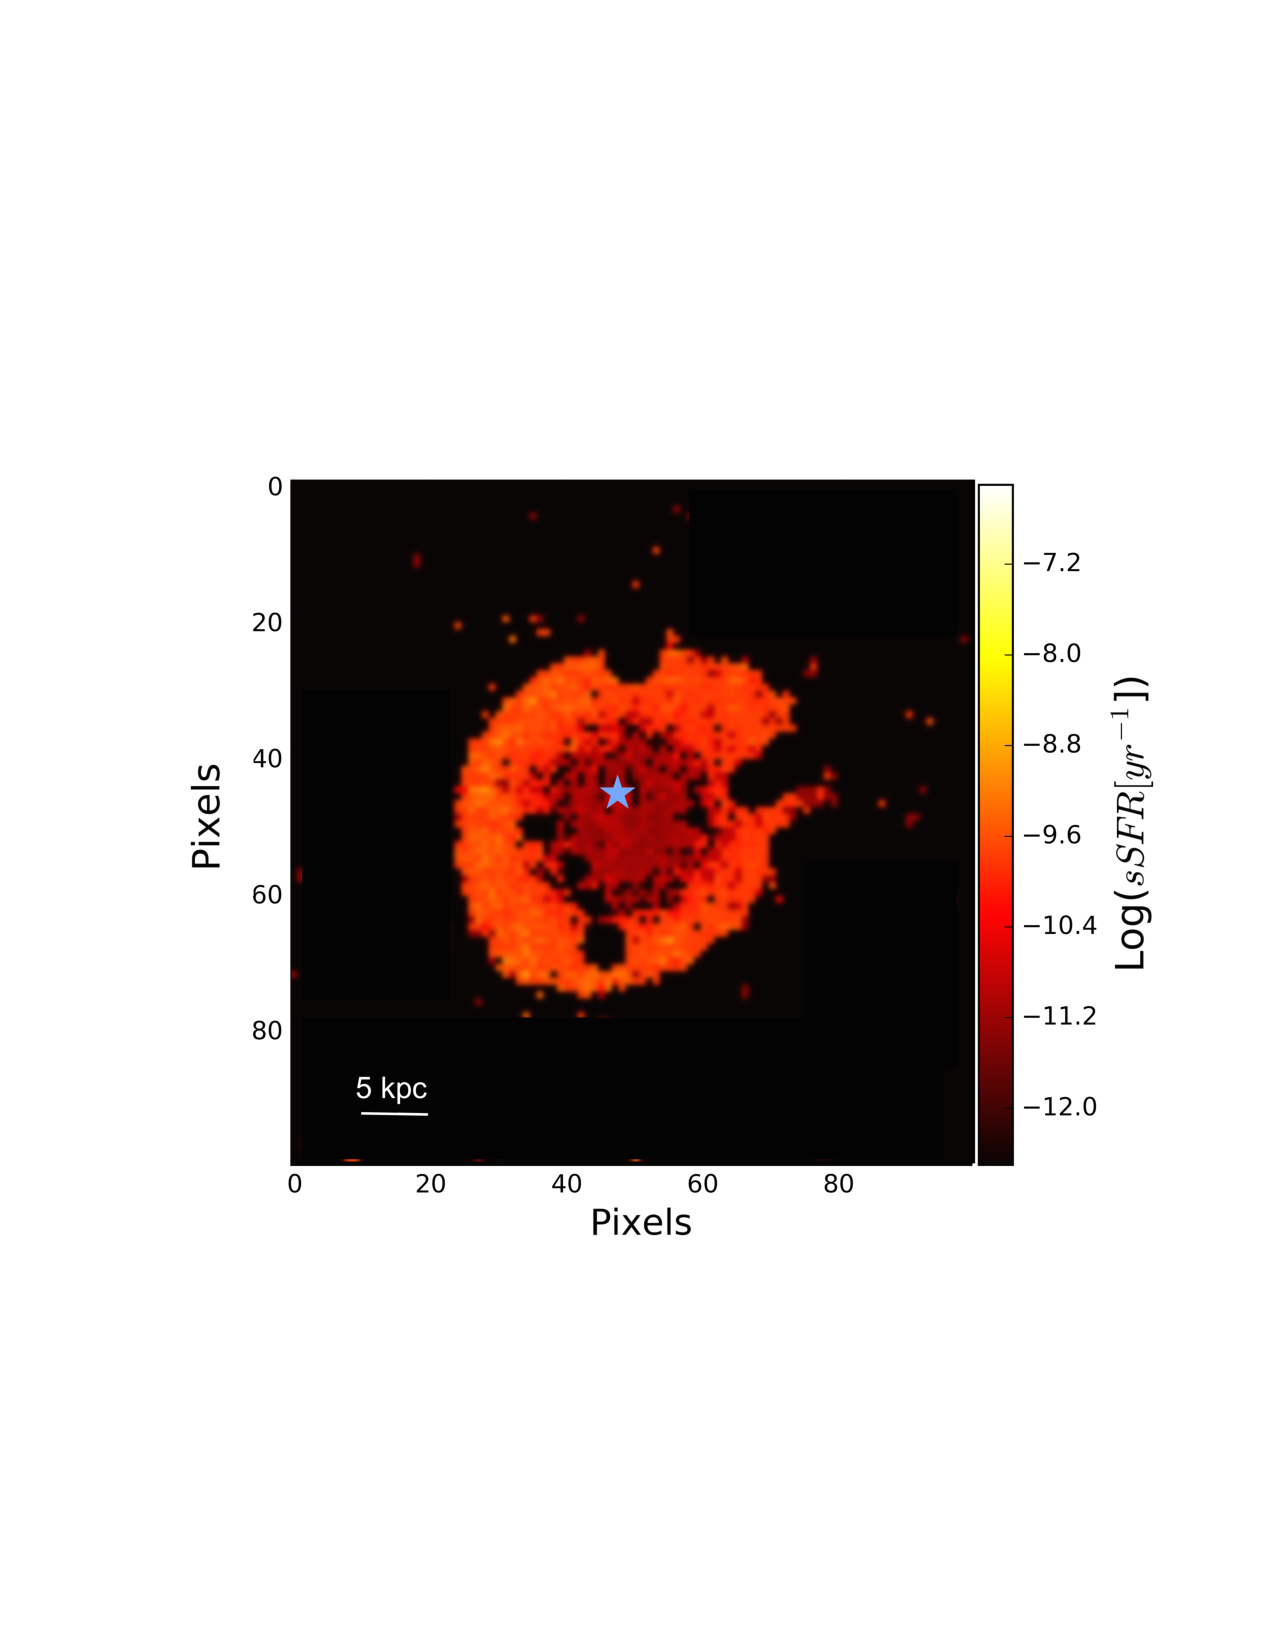
\includegraphics[width=0.55\textwidth]{./chapters/chapter3/Figures/f4a.pdf}\hspace{-0.55cm}\vspace{0.5cm}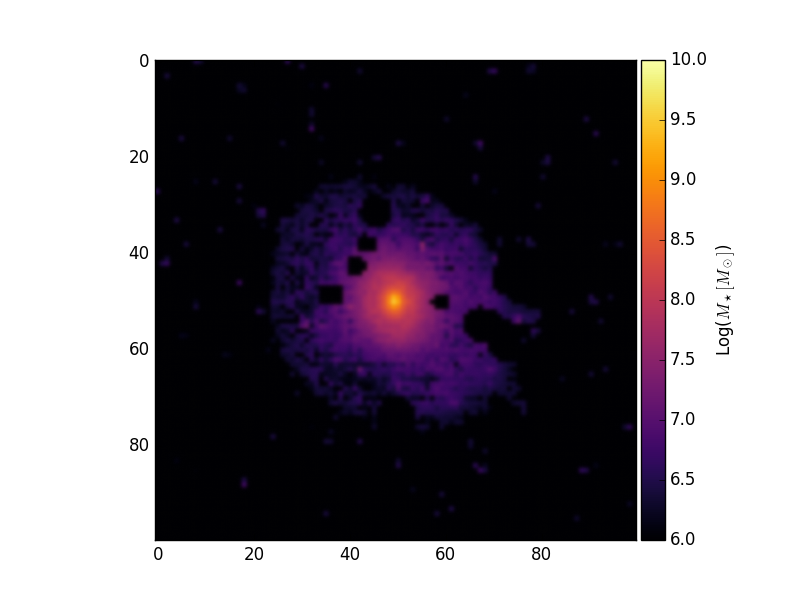
\includegraphics[width=0.55\textwidth]{./chapters/chapter3/Figures/smass_map_masked.png}
\caption{sSFR (left) and stellar mass (right) maps resulting from the pixel SED fitting of DES+VHS bands. Other objects have been masked out. $x$ and $y$ axes correspond to the map pixels. One pixel corresponds to a physical size of 0.526 kpc at the galaxy redshift. }\label{smass_map}\end{figure}

\begin{figure}
\centering
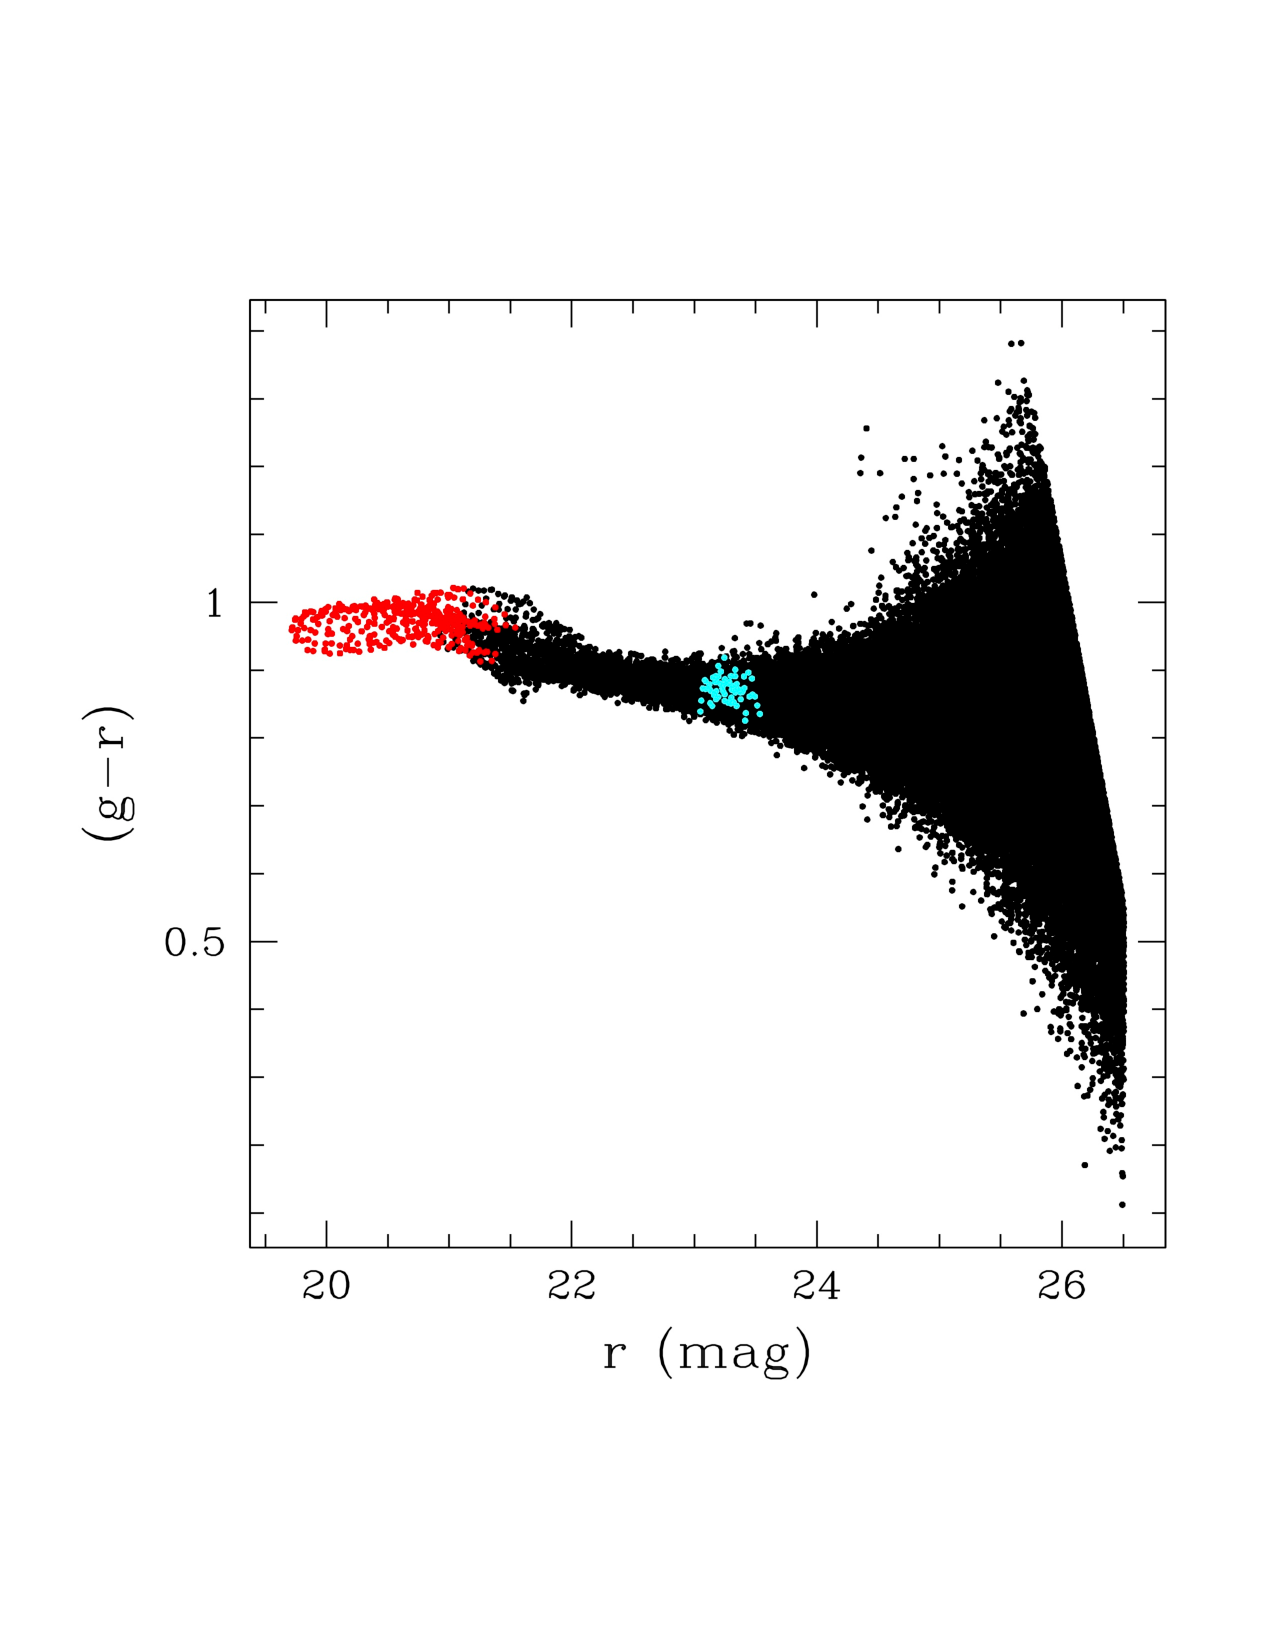
\includegraphics[width=0.55\textwidth]{./chapters/chapter3/Figures/f4b.pdf}
\caption{Pixel color-magnitude diagram for the pixels covering NGC4993 from DECam $g$ and $r$ single epoch exposures taken previously to the BNS event. The core of the galaxy is shown in red, while the cyan points represent the $1.5''$ around the location of the BNS event ($10.6''$ from the center).}\label{fig:pcmd}\end{figure}


\subsubsection{SED fitting results}\label{resultssec}
Figure \ref{spec} shows the best fit model of the 6dF spectrum, which results in a reduced $\chi^2$ of 1.22. An analysis of the mass fraction in age shows that part of the core galaxy stellar population has a supersolar metallicity, but the weighted mean value $\langle [M/H]\rangle=-0.012\pm 0.010$ is marginally consistent with solar metallicity. The mean age is $11.298\pm 0.054$ Gyr, and the mass-to-light ratio is $5.23\pm 0.15$ in $r$-band.

The stellar model fit reveals the existence of weak ionized gas emission lines. However, the line ratios from the fit suggests they are produced by a harder ionizing source than star-formation, formally lying in the AGN region of the Baldwin, Phillips \& Telervich (BPT; \citealt{BPTref}) diagram. \citet{blanchard} argue that there is a weak AGN present in the core of the galaxy on the basis of radio and X-ray emission, and so we conclude there to be no evidence of recent star-formation from the 6dF spectrum, irrespective of the highly uncertain ${\rm O\,\textsc{iii}}/H_\beta$ ratio. A comparison of galaxies in the group using AAT spectra and classification by \citet{2006MNRAS.372..961K} is shown in Figure \ref{fig:bpt}.

Given the evidence of dust presence in the HST study, we estimate the dust content using the Balmer decrement \citep{berman} observed from the spectrum. The reddening is $E(B-V)=0.12\pm 0.50$ in the case of $I(H_\alpha)/I(H_\beta)= 3.1$, which is expected in the case of AGN activity. We therefore restrict our dust models to have reddening values $0.1,0.2,0.3,0.4,0.5$ in the photometric fits.

The photometric best--fitting template has a solar metallicity, a quickly declining log-normal SFH with $t_0=3 \,{\rm Gyr}$ and  $\tau=0.1$. A low reddening $E(B-V) =0.1$ is preferred, and the stellar mass is $(2.95\pm 0.65)\times 10^{10}M_\odot$. The inclusion of a late SFH burst is disfavored by the fitting apart from intermediate apertures. 

Previous work found that the presence of dust lanes may bias the galaxy stellar mass from unresolved galaxy SED fits to lower values (\citealt{sorba}). The total stellar mass from fitting over the \sextractor segmentation map of NGC4993 is $(3.8\pm 0.20)\times 10^{10} M_\odot$, more than $1\sigma$ higher than the unresolved SED fitting. The specific SFR (sSFR) and stellar mass maps from our pixel SED fits are shown in Figure \ref{smass_map}, where the shell structure is clearly visible, suggesting that the sSFR is slightly more accentuated in the stellar halo compared to the inner parts. Younger ages (by $\sim 2~{\rm Gyr}$) are also preferred in the outer regions, though we still do not find evidence for a star formation burst at late times, and explain our results by the stripping of stellar populations from the lower-mass galaxy in a minor dry merger. A dust model with $E(B-V)=0.1$ is preferred in the inner few kpc, while $E(B-V)=0$ is found outside. Despite the presence of dust lanes, an analysis of the HST photometry and a comparison with extinction models suggests that the effect of dust is not extreme, with reddening values that are consistent with 0.1 in the core. We therefore believe that the dust obscuration does not play a significant role in our SFR estimates.


\subsubsection{Pixel Color Diagrams}
In Figure \ref{fig:pcmd} we show a color-magnitude diagram for all the pixels within the field of view of the DECam data near the galaxy. The image has been cleaned of stars and other contamination, thus all points come from the galaxy itself. The position of the GW source, $10.6''$ offset from the center, is the cyan colored pixels, while the center of the galaxy is shown in the red points. This galaxy is well represented by a pixel ``main sequence'' that is bluer at fainter levels, which is typical of early--type galaxy color gradients (e.g., \citealt{lanyon-foster}). We conclude that there is no significant difference between the transient position and other outer light, although it is bluer than the core region. This further supports the scenario in which the BNS formation is not related to some particular recent star formation event in this region.


%%%%%%%%%%%%%%%%%%%%%%

\subsection{Implications for the binary neutron star fomation and coalescence}\label{implications}

\subsubsection{BNS formation and delay time under the hypothesis of galaxy merger}

In the most accepted shell formation scenarios the shells are stellar debris coming from the less massive, stripped galaxy, and the arcs form at the apocenter of the orbits of the infalling material \citep{quinn}. The kinematics of the shells allow to connect their position, the gravitational potential of the galaxy and the time elapsed since the galaxy merger (\citealt{1986A&A...166...53D,2012A&A...545A..33E}).

Based on our results, we believe that NGC4993 experienced a dry minor galaxy merger with still visible signs. The shells are expected to be washed out within a time that depends on the velocity dispersion at their position. We estimate the shell survival time in two ways, based on the velocity dispersion of the galaxy as well as the velocity dispersion of the shell itself. From the 6dF spectrum the  line--of--sight central velocity dispersion is $\sigma_v=(160.0\pm 9.1)~{\rm km\, s^{-1}}$. We estimate its value at the position of the transient. 
The velocity dispersion of early type galaxies drops from its central peak value at larger radii, and observations show that the maximum drop to the outer parts of ellipticals near the effective radius is $\sim 40\%$ of the central value (\citealt{emsellem}). Based on the distance of the shell from the center, $R \approx  4 ~{\rm kpc}$, we estimate that the dynamical time at this radius is
$t_{\rm dyn} \equiv  R/\sigma_{v} \approx 60 ~{\rm Myr}$ (the line-of-sight velocity is relevant here, given the shell's geometry, but e.g. if we assume a 3D isotropic velocity dispersion it would reduce the dynamical time by $\sqrt{3}$).

So far we have no measurement of the shell's velocity dispersion, but estimates from the literature suggest for similar shells in other galaxies
$\sigma_v \approx  20 ~{\rm km\,s}^{-1}$ \citep{quinn}. This would give a dynamical time scale of $t_{\rm dyn} \approx  192~ {\rm Myr}$. 
Detailed simulations of  shells in other galaxies suggest that survival time could be even larger that 1 Gyr,  depending on the assumed scenario \citep{pop}.

The survival time of the shell could be used as an upper limit for the time the minor merger took place, i.e  $t_{\rm dyn} \geq t_{\rm merg} $, so we estimate $t_{\rm merg}  \lesssim  200$ Myr.

If the BNS was formed as such in a shell, then we would have expected to see evidence for recent star formation, but we find no indication of this. In the absence of star formation it is plausible that the BNS coalescence was triggered by a dynamical process, e.g. NS-NS capture or the destabilization of a pre-existing wide-separation binary. These processes will be quite sensitive to the stellar density which, given the S\'ersic index and the luminosity from the residual image found in section \ref{morphresults}, is high in the center of NGC4993 and around the transient position. If this dynamical hypothesis is true, then the delay time $\Delta t_{NSM}$ between the BNS formation and coalescence is $\lesssim 200~{\rm Myr}$. Figure \ref{timeline} shows a schematic timeline of the events described for NGC 4993.

\begin{figure}
\centering
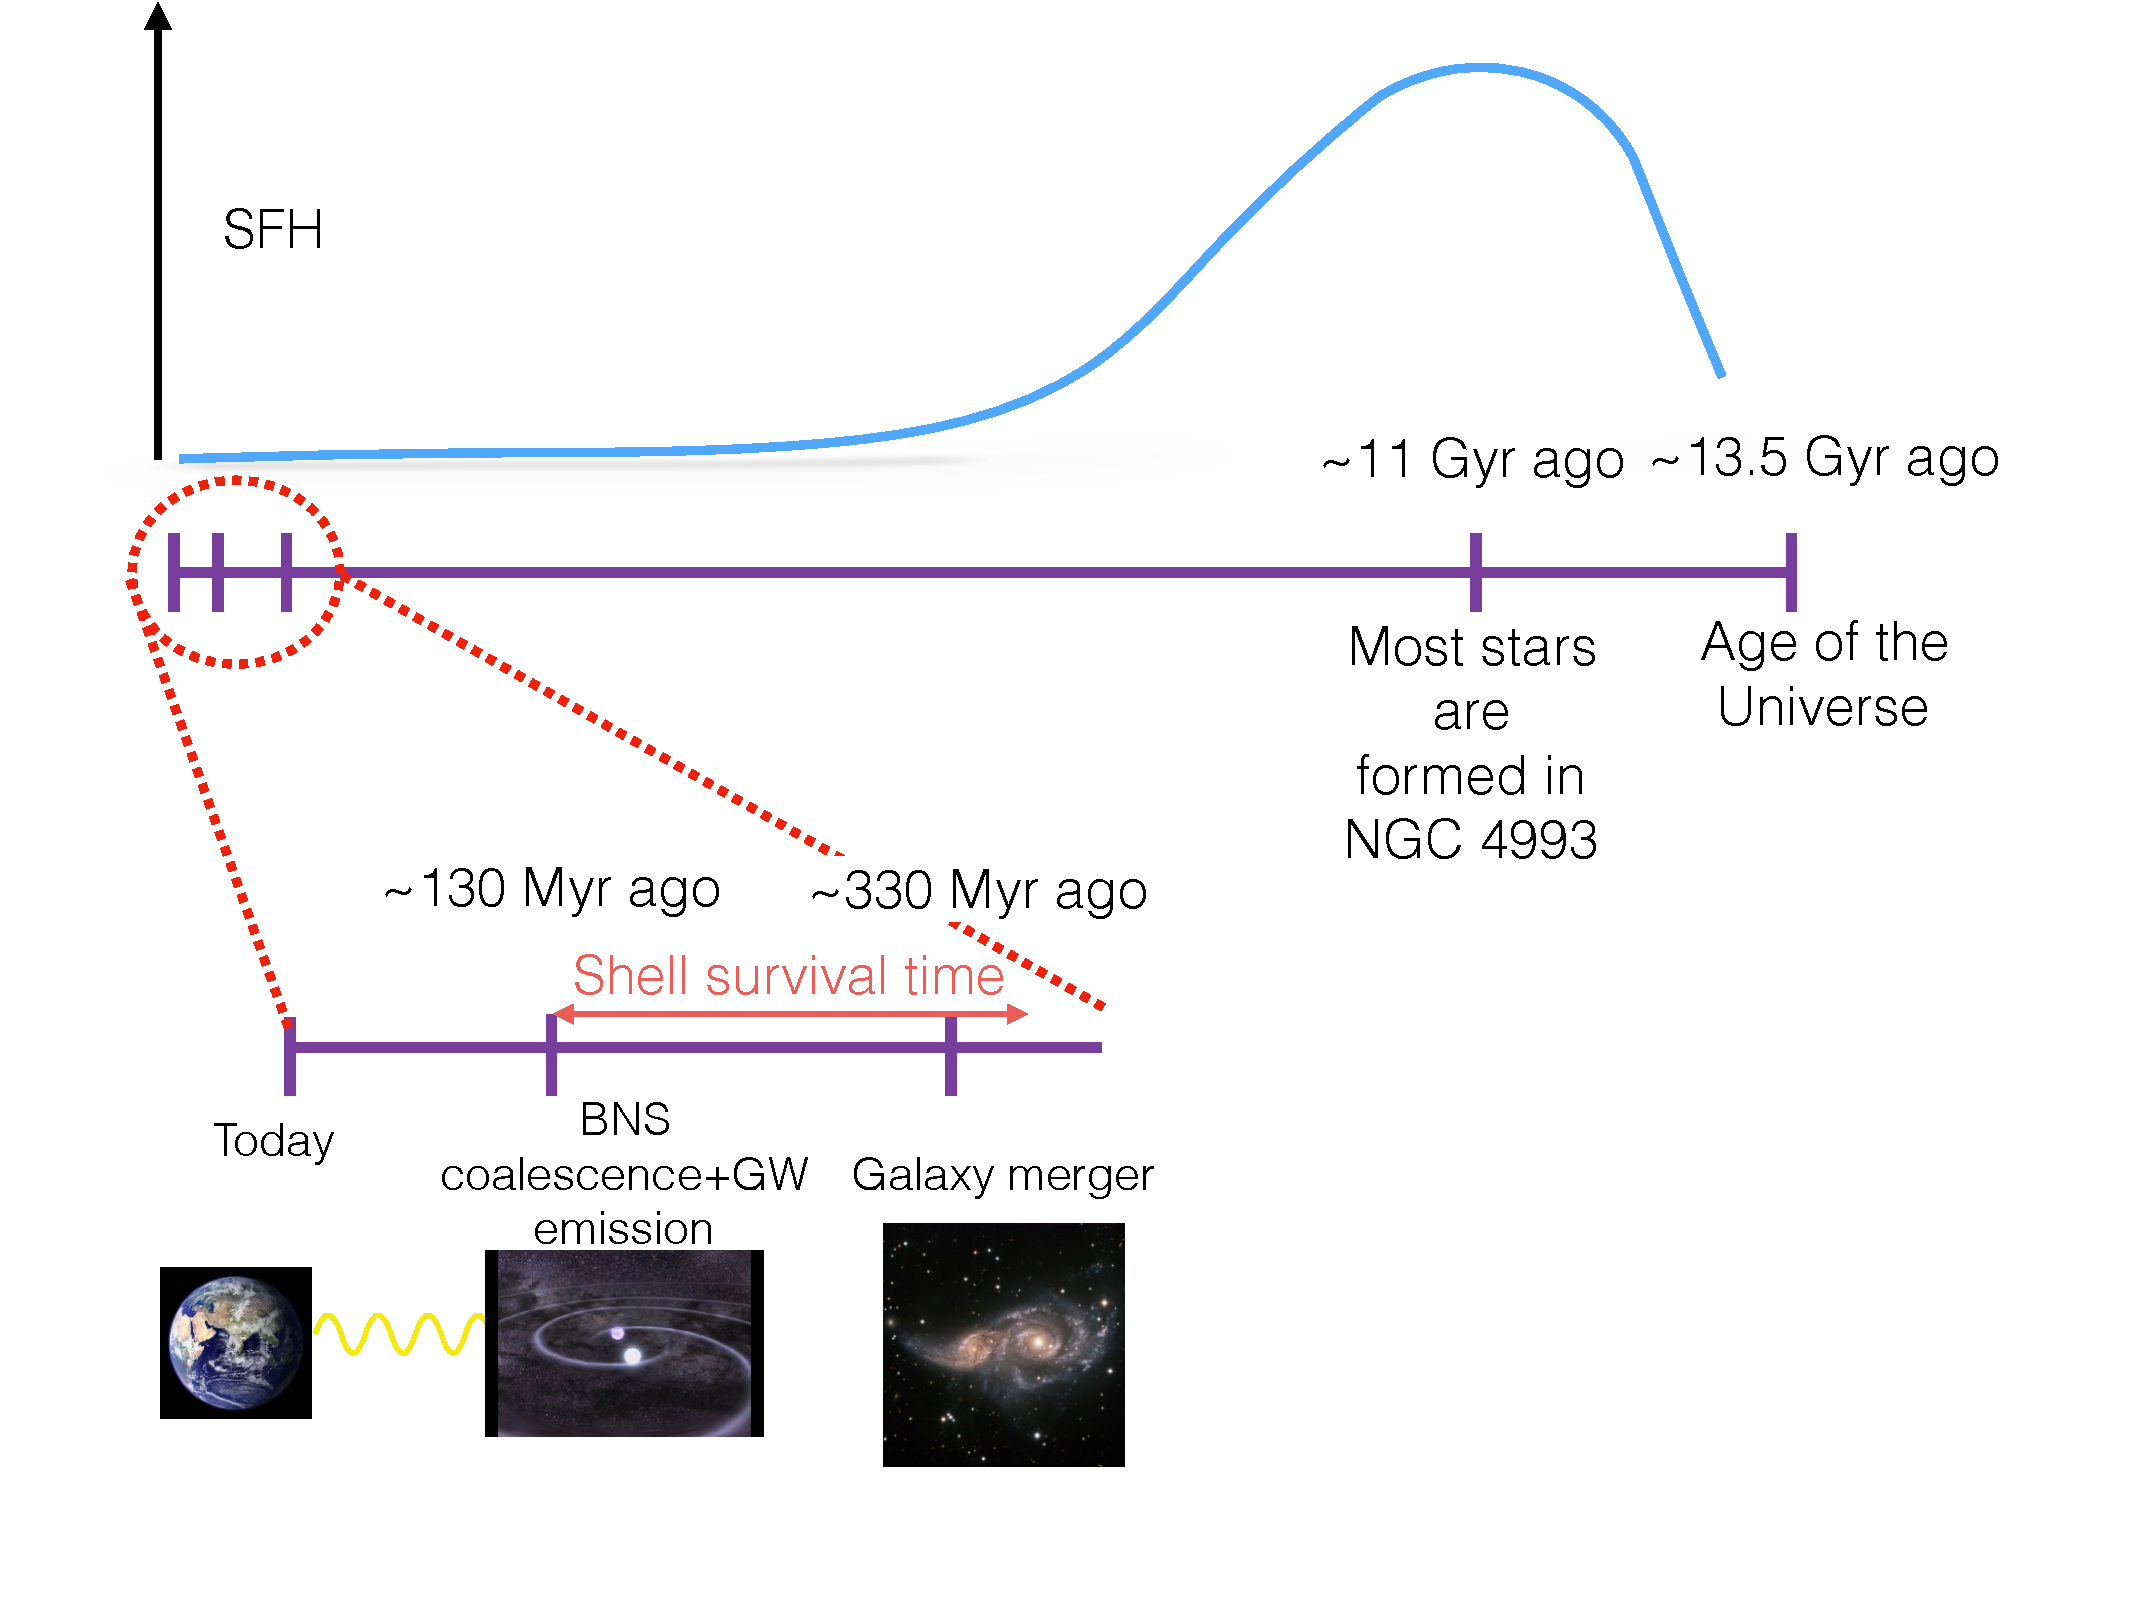
\includegraphics[width=0.85\textwidth]{./chapters/chapter3/Figures/timeline.pdf}
\caption{A schematic timeline of events for NGC 4993.}\label{timeline}\end{figure}


\subsubsection{Galaxy environment}
If the binary formation is related to dynamical processes in galaxy merging as we are investigating here, then this is most likely to happen in galaxy groups and low mass clusters.
According to the 2MASS catalog \citep{tully}, NGC4993 resides in a group, of which we analyze the remaining 7 galaxies. A spectral analysis shows that NGC4993 is not the only galaxy showing AGN activity (see Figure \ref{fig:bpt}), but it is peculiar in terms of age, metallicity and mass-to-light ratio. It shows an older stellar population (the mean age of the other 13 galaxies is ${\rm Log} (Age) = 9.56\pm0.17$), lower metallicity (mean: $M/H=-0.31 \pm 0.11$), and higher $M/L_r$ (mean: $2.41\pm0.45$ ) than the average. The group has a projected virial radius of $R_{vir} = 0.36$ Mpc and a line-of-sight velocity dispersion $\sigma_v = 143~ {\rm km\, s^{-1}}$ (\citealt{tully}). The crossing time is therefore $t_{\rm cr} \sim R_v/(\sqrt{2.5}\sigma_v)\sim 1.6$ Gyr.  

If galaxy mergers are correlated to BNS coalescence, future GW studies could possibly concentrate on galaxy groups (but note that these are crowded regions and therefore matching candidates to a host could be difficult). In order to have precise measurements of $H_0$, one needs to identify the host galaxy redshift clearly. When the match is clear, the properties of the type of host galaxy found could help future studies to select the right host galaxy or create galaxy catalogs of likely hosts for GW EM follow-up and untriggered kilonova searches (\citealt{doctor}). In fact, large photometric surveys such as DES, LSST or WFIRST are expected to observe kilonova events at redshifts beyond the sensitivity of GW experiments, where the angular separation between galaxies decreases (\citealt{scolnic}).


\subsubsection{BNS merging constraints}
We derive a constraint on neutron stars merging rate at time $t$ by using:
\begin{equation}
R_{NSM}(t) = \alpha R_{NS}(t')\, ,\label{rate}
\end{equation}
where $\alpha$ is the fraction of neutron stars which are in binaries, $t' = t-\Delta t_{NSM}$ and the fraction of mass of formed stars that are NS is: 
\begin{equation}
R_{NS}(t') = \int dM_\star \Phi(M_\star)\Psi(t_\star)\Theta_{NS}(M_\star)\, ,
\end{equation}
with $\Phi(M_\star)$ being the IMF, $\Psi(t_\star)$ is our best fit SFH, $\Theta_{NS}(M_\star)$ is 1 for star mass ranges of $8\, M_\odot<M<20 \,M_\odot$, zero otherwise. We drop the metallicity dependence in $\Theta_{NS}$ because we only consider a solar metallicity for the galaxy, as a result of our spectroscopic fit. $t_\star$ is the time when the progenitor of the NS was formed, therefore satisfying $t' = t_\star+t_{\rm life}$, with $t_{\rm life}$ being the lifetime of the progenitor before becoming a NS. We assume a $t_{\rm life}=0.02$ Gyr, but our calculation is insensitive to this choice as the typical lifetime of these massive stars ($\sim 0.01-0.03$ Gyr) is much shorter than the timescale over which the SFH found for NGC4993 is changing at late times.
We assume a Chabrier IMF, but this choice is not relevant as  we are only exploring the high mass end of the IMF. Assuming $\alpha=0.002$ and the distribution of $\Delta t_{NSM}$ from \citet{vangioni} (their Figure 3 for solar metallicity), and our best fit SFH from Eq. \ref{sfr} with $t_0=3 {\rm Gyr}$ and $\tau=0.3$, we get a NS formation rate of $R_{NS}^{\rm gal}= 3.6^{+28}_{-3.6} \times 10^{-5} ~{\rm yr}^{-1}$ and a BNS merger rate of $R_{NSM}^{\rm gal}= 5.7^{+0.57}_{-3.3} \times 10^{-6} ~{\rm yr}^{-1}$ for the whole galaxy. Errors reflect the uncertainty on the SFH, which dominates our errors: they represent the two central quartiles of the rates distribution computed with the SFHs of the pixel SED fitting over the galaxy.

Given the sensitivity of the BNS merger event rate to the recent SFR of a galaxy, it is somewhat surprising that GW170817 occurred in an old, early type galaxy. We therefore ask what is the probability of observing such an event in any early--type galaxy within the LIGO--detectable volume. To make this estimate we integrate the stellar mass function of early--type galaxies from \citet{weigel} and scale the per--solar--mass rate from Eq. \ref{rate} to the mass contained within the LIGO detectable volume (radius $80~{\rm Mpc}$). We find $R_{NSM}^{\rm early}= 23^{+2}_{-14} ~{\rm yr}^{-1} {\rm Gpc}^{-3}$ resulting in $0.038^{+0.004}_{-0.022}$ expected events. This calculation assumes that the SFH of NGC4993 is representative of local early--type galaxies. In fact much of the mass will be contained in more massive, and on average older and less star--forming, galaxies. We contrast this with a similar calculation for all galaxy types, using the cosmic SFR density from \citet{lognorm}, finding $R_{NSM}^{\rm all}\approx 270 ~{\rm yr}^{-1} {\rm Gpc}^{-3}$ and $\sim 0.5$ expected events.

\begin{figure}
\centering
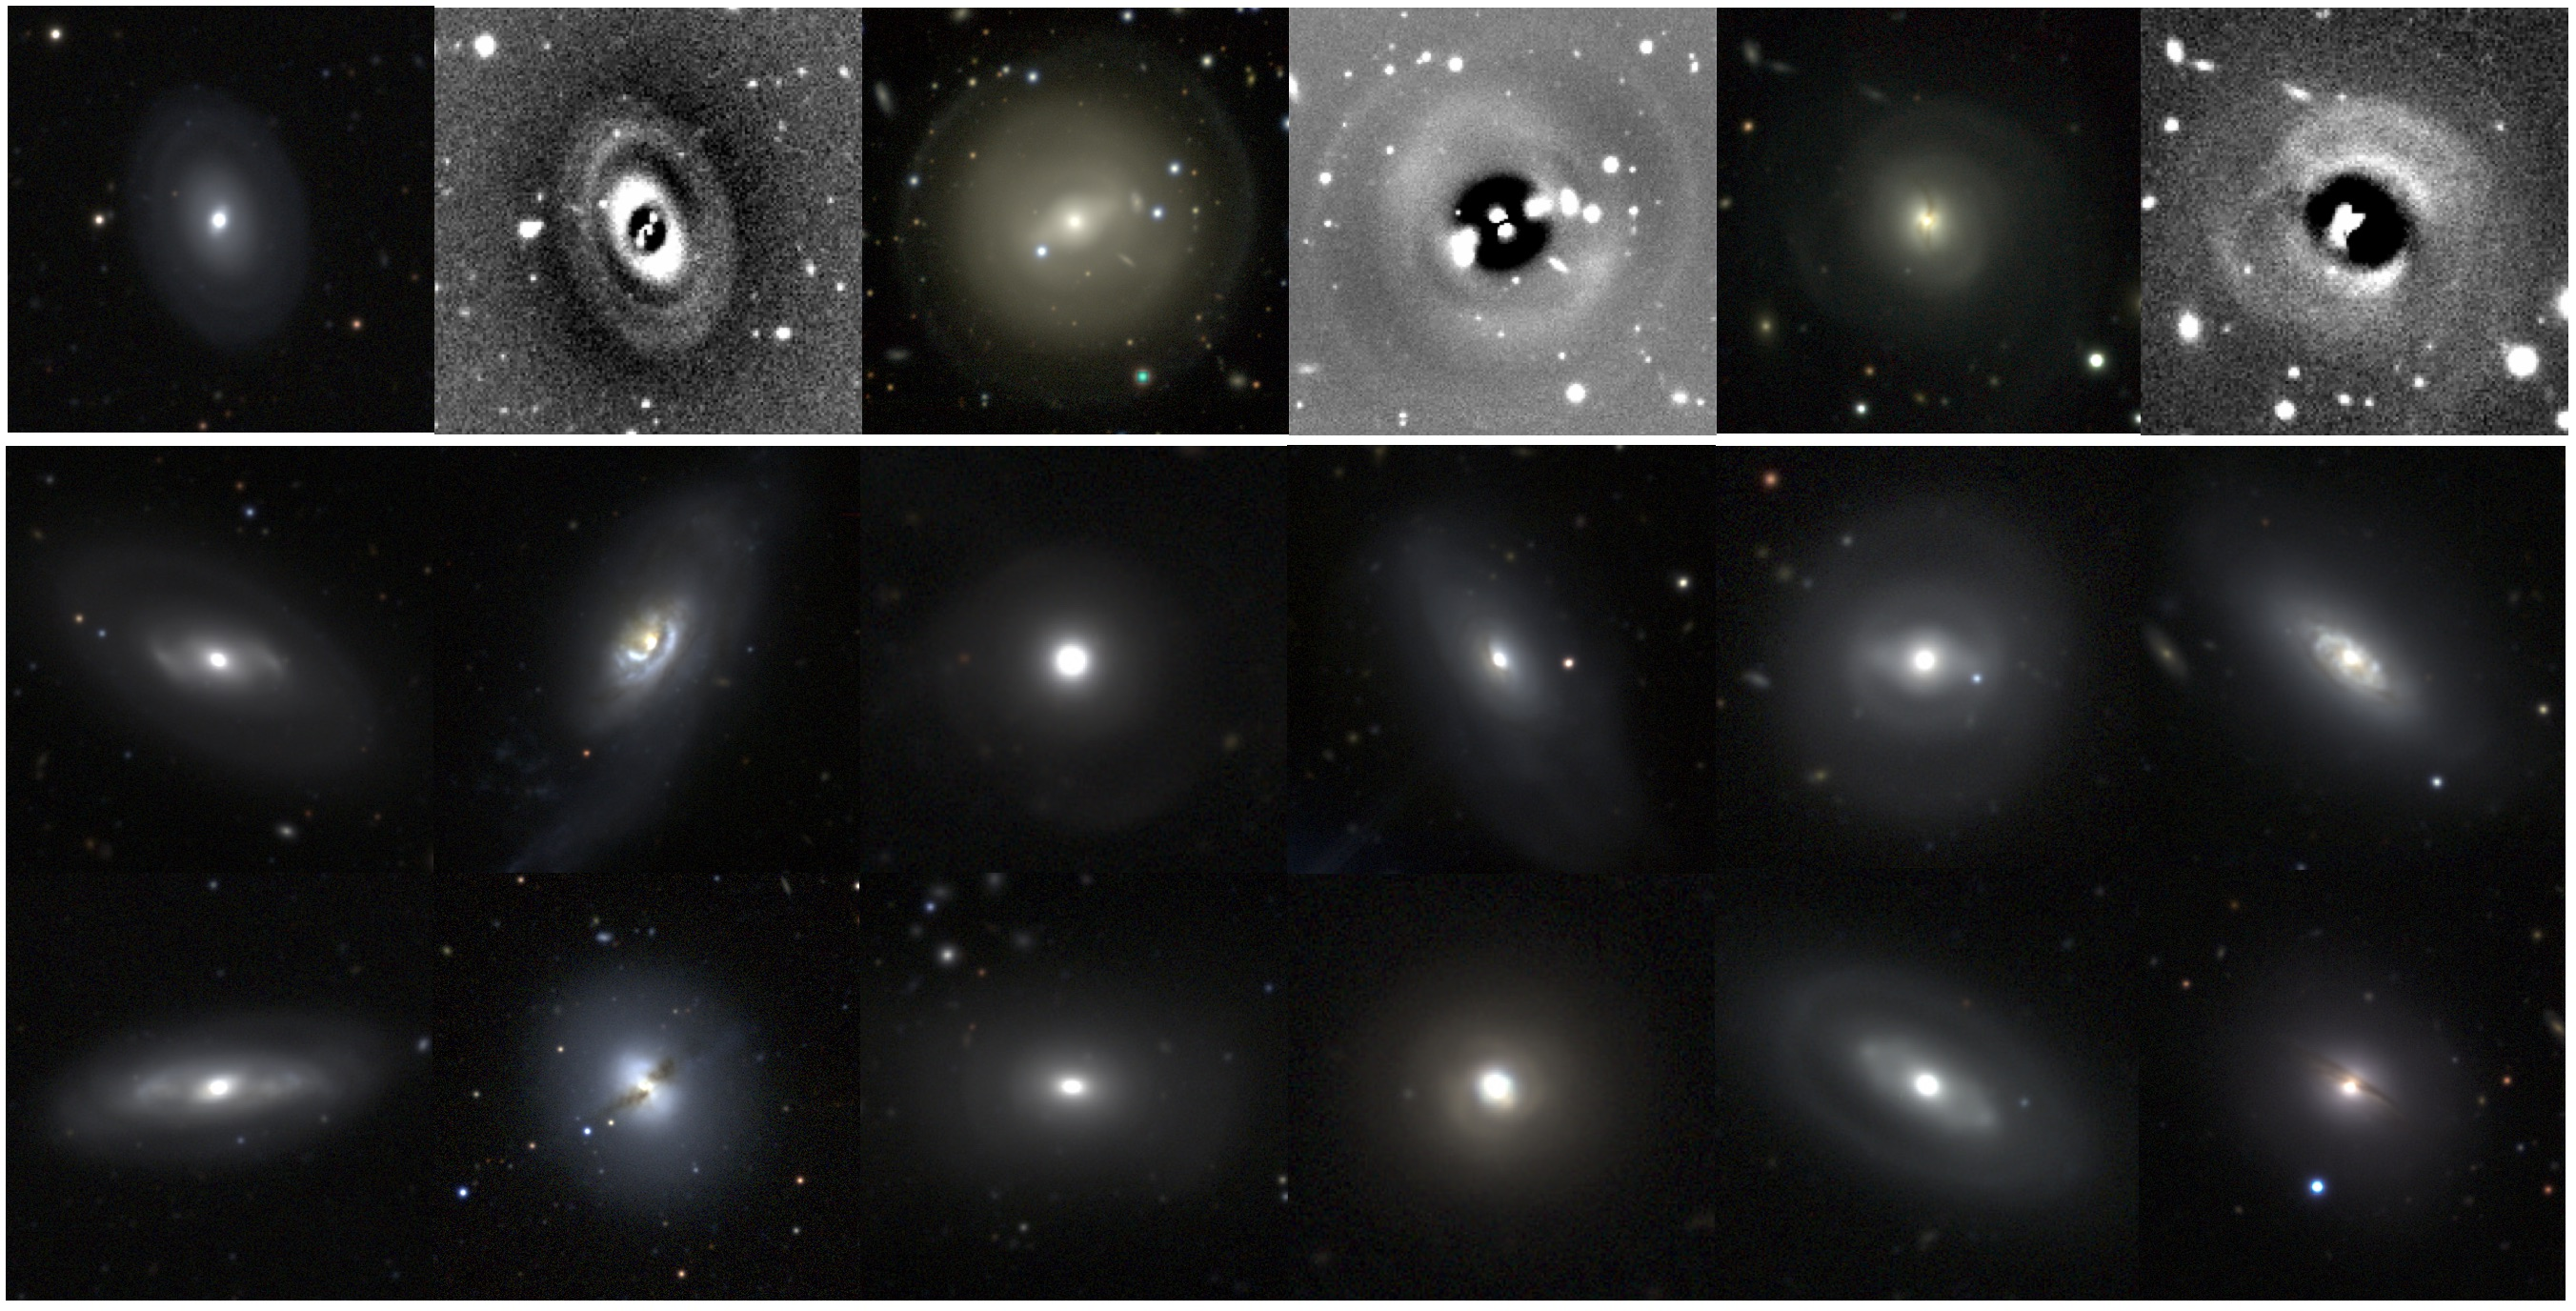
\includegraphics[width=1.\textwidth]{./chapters/chapter3/Figures/Y1SampleLight.jpg}
\caption{Sample of galaxies from DES Year 1 data with available \textsc{GalFit} parameters, having size, surface brightness and S\'ersic index within $10\%$ of the best fit values for NGC4993. Roughly $15\%$ of them present shell structures, while in the remaining galaxies we find also some spirals and barred spirals. In the top panels we show also the corresponding residual images for three galaxies from this sample. The first two clearly show shell structures, while the third also shows dust lanes. }\label{fig:shelly1}\end{figure}

This result shows that it is unlikely that we observed one such BNS merger with LIGO over the combined nine months of operations in an early--type galaxy. The assumptions in the calculation include the fraction of NS that form in binaries ($\alpha=0.002$) and the delay time distribution, both coming from binary star models (where the progenitors of the BNS were already a bound system) and satisfying Milky Way constraints. If the BNS formation mechanism is via dynamical interaction, our result could point to a higher value of $\alpha$ or a shorter $\Delta t_{NSM}$ for systems that recently underwent a galaxy merger, more so for those that have high stellar density (such as early--type galaxies). It is therefore of interest to know the fraction of galaxies similar to NGC4993 that show similar signs of a galaxy merger in the form of visible shells. We select galaxies from the first year of DES data with size, surface brightness and S\'ersic index within $10\%$ of the best fit values for NGC4993. We find $1100$ such galaxies, and visually inspect them to identify shell galaxies. A subsample of those is shown in Figure \ref{fig:shelly1}. Only $15\%$ of these objects display shells, and so NGC4993 is unusual amongst early-type galaxies.

On the other hand, \citet{blanchard} find a median delay time of $11^{+0.7}_{-1.4} {\rm Gyr}$ under the assumption that the binary was formed through secular SF, and that no interactions disturbed the binary since it was formed. This is derived from the measured SFH, which is similar to what we find, and from which they find that $50\%$ of the stellar mass of NGC4993 was formed $11^{+0.7}_{-1.4} {\rm Gyr}$ ago. This scenario is possible and cannot be excluded, although our study shows that it is unlikely.

Our results are far from conclusive evidence for a merger origin of BNS events. However, the coincidence of evidence for a recent merger in a galaxy for which a BNS event was otherwise improbable is compelling.

\section{Conclusions}

In this Chapter we have shown how galaxy properties are important not only for GW electromagnetic follow up strategies, but also to study the formation and evolution of the GW sources. In particular, we can use the SED fitting results that we get from the methods described in the previous Chapter to:
\begin{itemize}
\item Match to galaxies the transients found from GW follow up searches. The goal of this search is twofold. First, by identifying a GW source host with a photo-$z$ or spectroscopic redshift, we can relate it to the distance provided by LIGO and use the GW event as a standard siren and measure cosmological parameters. Secondly, we can identify and reject Supernovae that contaminate our candidate list and restrict our analysis to a smaller sample.
\item Study binary systems formation and evolution. In the case of GW170817, the star formation and the properties of the host galaxy showed that the fact that this event happened in NGC4993 was unlikely based on current BNS models. These models, based on pure star formation, should be revisited in the future. Other works followed our line of thought and reached similar conclusions (\citealt{Belczynski}; \citealt{ebrova}).
\item Constrain the delay time of the GW sources, either through estimating a time for dynamical interactions in the case of dynamically--driven formation of the system (as in Palmese et al. 2017), or through a study of the star formation history (as in \citealt{blanchard}).
\end{itemize}

Furthermore, galaxy catalogs such as the one described in this Chapter, can be used to point small FoV telescopes after a GW trigger towards galaxies with the properties that are most likely to be those of the host of the event. For example, one could assume that these events are most likely to happen where most of the stellar mass is, or in the most luminous or star--forming galaxies. However, only further follow ups will provide some statistics and will allow us to identify the galaxy properties of the most likely hosts.







\clearemptydoublepage
\chapter{Stellar mass versus dark matter in galaxy clusters: RXJ2248}\label{chp:rxj}

\begin{flushright}
  {\em ``I have forced myself to contradict myself in order to avoid conforming to my own taste.''}\\
  
\ \

\normalsize
{Marcel Duchamp}  
\end{flushright}


\noindent{\emph{The work described in this chapter is part of {\bf Palmese et al., 2016, MNRAS, 463, 1486}.}
%\begin{abstract}
%We derive the stellar mass fraction in the galaxy cluster RXC J2248.7--4431 observed with the Dark Energy Survey (DES) during the Science Verification period.  We compare the stellar mass results from DES (5 filters) with those from the Hubble Space Telescope CLASH (17 filters). When the cluster spectroscopic redshift is assumed, we show that stellar masses from DES can be estimated within 25\% of CLASH values. 
%We compute the stellar mass contribution coming from red and blue galaxies, and study the relation between stellar mass and the underlying dark matter using weak lensing studies with DES and CLASH.  An analysis of the radial profiles of the DES total and stellar mass yields a stellar-to-total fraction of $f_\star=(6.8\pm 1.7)\times10^{-3}$ within a radius of $r_{200c}\simeq 2$ Mpc. Our analysis also includes a comparison of photometric redshifts and star/galaxy separation efficiency for both datasets. 
%We conclude that space-based small field imaging can be used to calibrate the galaxy properties in DES  for the much wider field of view. The technique developed to derive the stellar mass fraction in galaxy clusters can be applied to the $\sim100\, 000$ clusters that will be observed within this survey and yield important information about galaxy evolution.
%\end{abstract}


\section{Introduction}
In the last decade, large photometric galaxy surveys, such as SDSS, have provided us with a massive amount of data that have proven to be extremely useful for studies of cosmology. On the other hand, smaller area but deeper surveys like the Hubble Space Telescope (HST) based Cluster Lensing And Supernova Survey (CLASH) (\citealt{postman}), allowed us to characterise single objects with unprecedented precision. The importance of finding synergies between these surveys relates to several aspects of observation (e.g. target selection, photometric calibration) and data analysis (photometric redshifts, physical properties of galaxies). This is particularly relevant for overlapping ground--based and space--based surveys: the higher quality that can be obtained from space can enable calibration and tests for the data collected by ground--based telescopes. 

In this Chapter, we study the cluster of galaxies RXC J2248.7--4431 (RXJ2248 hereinafter). We make use of the synergies between DES and CLASH, and test in this way the performance of the early DES data at a catalog level (\emph{i.e.} without making use of the images for the results). Photometric redshift (photo-$z$) and stellar mass results from CLASH are also used as a validation set for DES stellar mass estimates.

The aim of this work is twofold: the first goal is to compare between DES's wide area breadth and CLASH's small area precision for the cluster RXJ2248. In fact, checks using HST data had not been done before to test the DES data, although the similar optical filters and the additional UV and IR HST bands make CLASH an optimal candidate for validation  and quantifying uncertainties of photometry, photo-$z$'s and stellar masses. The second is to illustrate how an analysis of the stellar mass distribution of this massive cluster over the wider Dark Energy Camera (DECam) field of view can be done. 

In Section \ref{observations}, we start by describing the two surveys considered. The cluster is described in Section \ref{previousworks}. The comparison of DES and CLASH, in terms of photometric redshifts and star/galaxy separation, is presented in Section \ref{comparison}. Section \ref{DMandSM} contains the second part of this work, where we present the stellar mass results obtained from CLASH and DES, and compare the DES stellar masses to the total mass from the DES weak lensing analysis by \citet{melchior}. 
In the following, we assume a concordance $\Lambda$CDM cosmological model with $\Omega_m =0.3$, $\Omega_\Lambda =0.7$ and $h=0.7$. In this cosmology, $1'$ corresponds to a physical transverse length of 295 kpc at the cluster redshift $z=0.3475$. 

%The notation adopted in this paper for the cluster mass and radius follows the one often used in literature. The radii of spheres around the cluster centre are written as $r_{\Delta m}$ and $r_{\Delta c}$ where $\Delta$ is the overdensity of the sphere with respect to the mean matter density (subscript $m$) or the critical density (subscript $c$) at the cluster redshift. Masses inside those spheres are therefore $M_{\Delta m}=\Delta \frac{4 \pi }{3}r^3_{\Delta m}\rho_m$ and similarly for $M_{\Delta c}$.  In the following, we quote $\Delta=200$, which is the density contrast at virialization for a dark matter halo.


\section{Data}\label{observations}
The data used for the analyses developed for this work come from DES and CLASH. %The Dark Energy Survey is an optical-near infrared survey that is imaging 5000 ${\rm deg}^2$ of
%the South Galactic Cap in the $grizY$ bands over 525 nights spanning 5 years. The survey is being carried out using a new $\sim 3$ $\textrm{deg}^2$ CCD
%camera (the DECam, see \citealt{flaugher}) mounted on the Blanco 4-m telescope at the Cerro Tololo Inter-American Observatory (CTIO) in Chile. DES started in 2012 with a testing period (November 2012 -- February 2013) called DES Science Verification (SV)\footnote{For public data release see: \url{http://des.ncsa.illinois.edu/releases/sva1}}. At the time of writing, two observing seasons (\citealt{y1}) have been completed, and a third is underway.

%The survey strategy is designed to optimize the photometric calibration by tiling each region of the survey with several overlapping pointings in each band. This provides uniformity of coverage and control of systematic photometric errors. This strategy allows DES to determine photometric redshifts of galaxies to an accuracy of $\sigma(z) \simeq 0.07 $ out to $z \gtrsim 1$, with some dependence on redshift and galaxy type, and cluster photometric redshifts to $\sigma(z) \sim 0.02$ or better out to $z \simeq 1.3$ (\citealt{descollaboration}). It will also provide shapes for approximately 200 million galaxies for weak lensing studies. For further information, see \citet{descollaboration} or \url{www.darkenergysurvey.org}. 

The fact that DECam has a $\sim 3$ $\textrm{deg}^2$ field of view gives us the opportunity of studying the large scale structure of galaxy clusters with only one pointing. 
\begin{figure}\centering
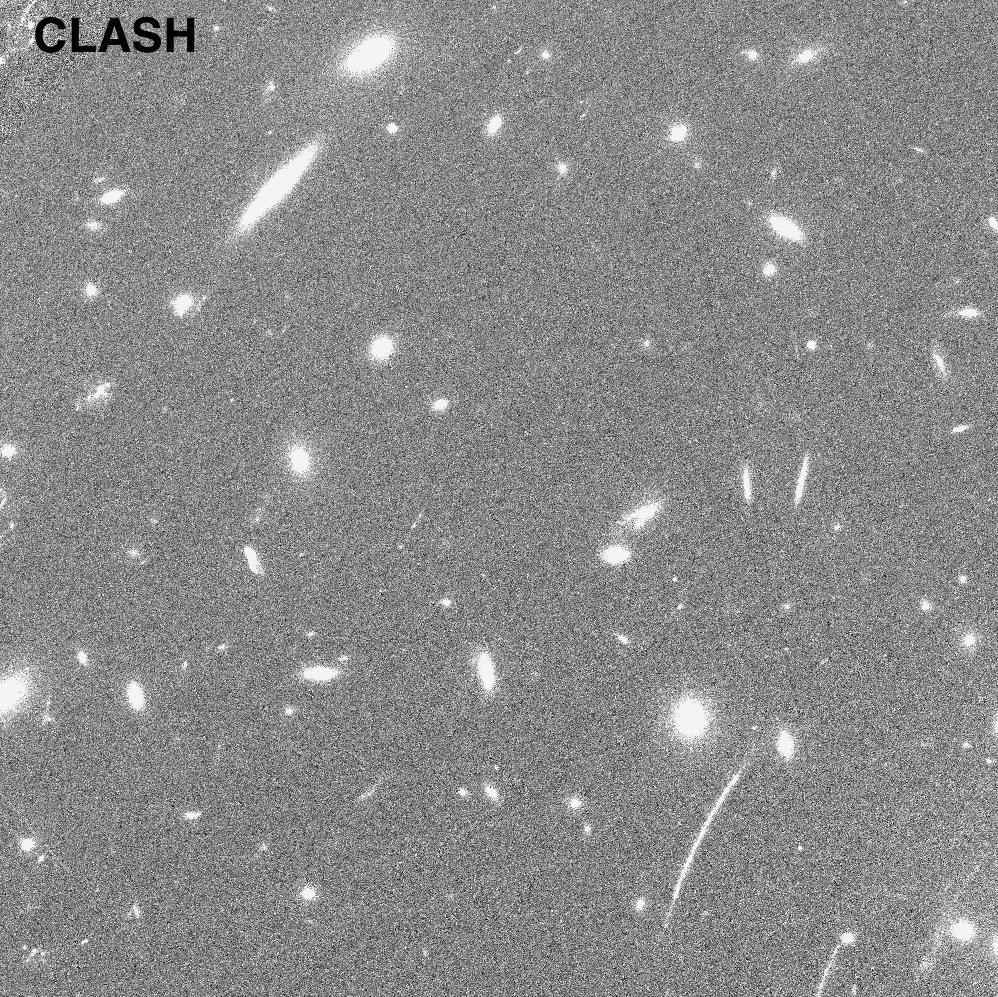
\includegraphics[width=0.5\textwidth]{/Users/apalmese/work/PhD_thesis/thesis_format/chapters/chapter4/Figures/clash_F625.jpeg}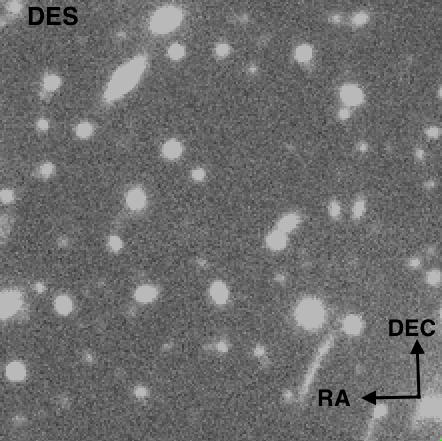
\includegraphics[width=0.5\textwidth]{/Users/apalmese/work/PhD_thesis/thesis_format/chapters/chapter4/Figures/des_r.jpeg}
\caption{A portion of $1'\times 1'$ image centered in RA 22:48:48.003 and DEC -44:31:38.52 in the CLASH F625W band (top) and the DES $r$ band (bottom).}\label{images}
\end{figure}
\begin{table}\centering
\begin{tabular}{cccc}
$\alpha_{J2000}$&$\delta_{J2000}$&Redshift& Luminosity (erg $\mathrm{s}^{-1}$)\\
\hline
22:48:44.29 &-44:31:48.4 & 0.348&$ 3.08 \times 10^{45}$
\\
\end{tabular}\caption{Main properties of the cluster RXC J2248-4431. The quoted luminosity is in the rest frame 0.1-2.4 keV band.}\label{properties}
\end{table}
\begin{table}
{\small
\centering
\begin{tabular}{c|cccccccc}
Survey/& Authors & FoV &Filters& Mag limits&Spectra&Objects\\
Instrument&&&&&&\\
\hline
NTT+&G12&$5'\times 5'$&$V$, $R$&--&116&711\\
GMOS&&&&&&\\
CLASH&P12&$3.4'\times3.4'$ (ACS), &16 in $2000-$&$\sim$ 25-27 ($10\sigma$)&-- &3471\\
& M14 &$2'\times2'$ (WFC3)&$17000\, \mathrm{\AA}$&&&\\
WFI&G13 &$33'\times 33'$& $UBVRIZ$&26.4, 26.7, &--&--\\
&&&&24.4 ($VRI$ $5\sigma$)&&&\\
DES & M16&2.2\,$\mathrm{deg}^2$&$grizY$& 24.45, 24.30,&--&$374\;294$\\
&&&&23.50,22.90,&&&\\
&&&&21.70 (10$\sigma$)&&&

\end{tabular}}\caption{Some experimental specifications of the surveys that have observed RXJ2248, with the corresponding paper in which those data have been used. The work presented in those papers is shortly summarised in Section \ref{previousworks}. G12, P12, M14, G13 and M16 stand for \citet{gomez}, \citet{postman}, \citet{monna}, \citet{gruen}, \citet{melchior} respectively. The magnitude limits reported for DES are the mean 10$\sigma$ galaxy magnitudes.}\label{surveys}
\end{table}

The cluster RXJ2248 was observed during the SV season, with typical exposure times of 90 seconds for the $griz$ bands and 45 seconds for the $Y$ band. It was re-observed later in 2013 to benefit from improvements to telescope performance and general image quality. The data reduction was done using the SVA1 DES Data Management (DESDM) pipeline, described in detail in \citet{sevilla}, \citet{desai} and \citet{dataproc}. The process includes calibration of the single-epoch images, that are then co--added after a background subtraction and cut into tiles. The SVA1 catalogue was created using \textsc{Source Extractor (SExtractor}, \citealt{sextractor1}, \citealt{sextractor}) to detect objects on the $riz$ coadded images. 
The median $10\sigma$ depths of SV data are $g\sim24.45, r\sim24.30,i\sim23.50,z\sim22.90, Y\sim21.70$, which reach close to the expected DES full depths. Limiting magnitudes were estimated for the 200 deg$^2$ SPT-E part of the wide--field SV area using \textsc{Balrog} (\citealt{suchyta}) and PSF magnitude errors for true point sources. 

We use AB magnitudes throughout this work, and \texttt{MAG\_AUTO} measurements given by \textsc{SExtractor}, as these proved to be robust and were thus used in several DES SV papers (e.g. \citealt{bonnett},\citealt{crocce}). The objects selected for the analysis have a signal to noise $S/N>10$ in the $i$ band.

The other survey considered here is CLASH (\citealt{postman}), a 524-orbit HST multi-cycle treasury program that has observed 25 massive clusters, having a range of virial masses between $5 \times 10^{14} M_\odot$ to $30 \times 10^{14} M_\odot$ and an average redshift of $\bar{z}=0.4$. The wavelength range covers the UV, the visible and the IR ($2000 - 17000 $ \AA) through 17 bands using the Advanced Camera for Surveys (ACS) and the Wide Field Camera 3 (WFC 3).

The CLASH mosaics were produced using the ``MosaicDrizzle'' pipeline (see \citealt{koekemoer02}, \citealt{koekemoer}). The CLASH catalogue creation pipeline makes use of \textsc{SExtractor}: the software is run in dual image mode, where a detection image is created from a weighted sum of the ACS/WFC and WFC3/IR images.  The WFC3/UVIS images are not used in the construction of the detection image but the UVIS data are still used to compute source photometry. The photometry given in the public catalogue (\url{http://www.stsci.edu/~postman/CLASH}), which is also the one used in this work, was measured in isophotal apertures, as they have been shown to produce reliable colours (\citealt{benitez}). ACS/WFC3 reach a depth of 26.8, 26.4, 26.2, 26.0 and 26.6 ($10\sigma$ galaxy AB magnitudes for circular apertures of 0.4 arcsec in diameter, \citealt{postman}) in the F475W, F625W, F775W, F850LP and F105W filters, respectively.

Below, we compare the information obtained with 5 DES filters and with 17 HST filters.

\section{The Cluster RXC J2248.7--4431}\label{previousworks}
In this section we present what is known about this cluster from previous works. The cluster of galaxies RXC J2248.7--4431, where RXC stands for ROSAT X-ray Cluster, is also known as Abell S1063 or MACS 2248--4431. It is a very luminous cluster, having an X--ray bolometric luminosity of $(6.95 \pm 0.1)\times 10^{45}\; {\rm erg\, s^{-1}}$ in the energy range $0.1-100$ keV (\citealt{maughan08}). Its properties are listed in Table \ref{properties}. It  was first catalogued by \citet{abell}, who counted 74 galaxies. Thanks to the ROSAT-ESO Flux Limited X-ray (REFLEX) Galaxy Cluster survey, \citet{bohr} measured a spectroscopic redshift $z=0.3475$, which has been adopted in the recent literature and has also been confirmed in \citet{gomez}, who quoted a mean redshift of $z=0.3461^{+0.0010}_{-0.0011}$ for 81 members.

\begin{figure}
\centering
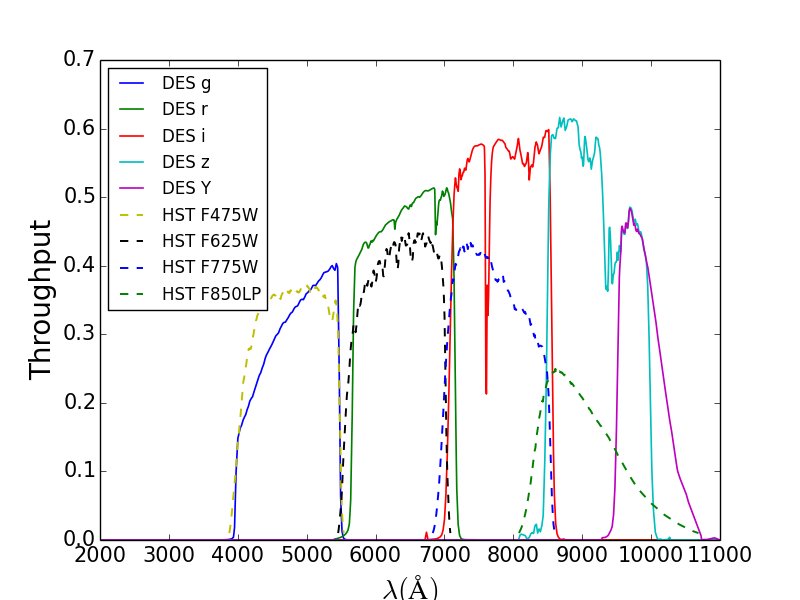
\includegraphics[width=0.5\textwidth]{/Users/apalmese/work/PhD_thesis/thesis_format/chapters/chapter4/Figures/filters.png}\caption{Throughput of the DES filters (solid lines) and HST similar filters (dashed lines).}\label{filters}
\end{figure}

\citet{gomez} were the first to study in detail RXJ2248, even though it is the second most luminous cluster in the REFLEX survey (having a reported luminosity of $\sim 3.08 \times 10^{45}$ erg $\mathrm{s}^{-1}$ in the rest frame $0.1-2.4$ keV band). 

In \citet{gomez}, the cluster is presented as one of the hottest X-ray clusters known at that time. The high X-ray temperature, together with the high velocity dispersion, suggest a very massive cluster ($M_{200\mathrm{c}}>2.5 \times 10^{15} \Msun$) and/or a merger system. The merger model is supported by a small offset between the galaxy distribution and the peak of X-ray isophotes, and a non-Gaussian galaxy velocity distribution. \citet{gomez} also reported that the velocity distribution is better represented by the velocity dispersion produced during a merger than by the velocity distribution of a relaxed cluster.

\citet{gruen} used Wide-Field Imager (WFI) data to perform a weak lensing analysis of the cluster. They parametrised the cluster density with a NFW profile (\citealt{nfw}) and obtained a mass $M_{200m}=33.1^{+9.6}_{-6.8}\times 10^{14}\Msun$ (or $M_{200c} = 22.8 ^{+6.6}_{-4.7}\times 10^{14} \Msun$). They also identified a second galaxy cluster in the field of view at redshift $\sim 0.6$, with an estimated mass of $M_{200m}=4.0^{+3.7}_{-2.6}\times10^{14}\Msun$.

\citet{melchior} studied the weak lensing masses and galaxy distributions of four massive clusters observed during the DES SV period, including RXJ2248. They found $M_{200\mathrm{c}}=17.5^{+4.3}_{-3.7}\times 10^{14} \Msun$, which is in agreement with previous mass estimates. For RXJ2248, they also identified filamentary structures of the luminous red-sequence galaxies found with the \textsc{RedMaPPer} (\citealt{redpaper}) algorithm. 

\citet{umetsu15} combined HST and wide field imaging (from the Subaru telescope or the ESO/WFI) observations to reconstruct the surface mass density profiles of 20 CLASH clusters. Their analysis jointly uses strong lensing as well as weak lensing with shear and magnification, and for RXJ2248 they found $M_{200c}=18.78 \pm 6.72 \times 10^{14}\Msun$.

\section{Comparison of DES and CLASH}\label{comparison}
In this section, we assess detectability, photometry, and stellar masses of DES galaxies, treating matched CLASH galaxies as truth table.\footnote{A comparison of weak lensing measurements between DES and CLASH was not performed because they predominantly reveal differences in the shear calibration. The majority of galaxies with shape measurement in both catalogs are very faint for DES, resulting in large and noisy calibration factors (see Section 4.2.1 in \citealt{melchior}). In addition, the high density of galaxies in the central region of this cluster creates many more close galaxy pairs or even blends in ground--based DES images than when viewed with HST, rendering shape measurement even more challenging. A detailed analysis of those relevant effects is beyond the scope of this work.} In order to make the comparison, we seek to identify similar filters in both data sets. Figure \ref{filters} shows that the closest HST analogs to DES $griz$ are F475W, F625W, F775W and F850lp. We will refer to the corresponding HST and DES bands as $g$, $r$, $i$ and $z$ for simplicity of notation. In the following, we will also use the DES $Y$ band, that does not have a similar HST filter. When we refer to 5 CLASH filters, it means we are including the F105W filter, that is broader than the DES $Y$. 

In the DES catalogue of the RXJ2248 area, there are $374\,294$ sources in a roughly circular area of approximately 3 $\mathrm{deg}^2$. 
The deeper, higher resolution CLASH catalogue includes $3\,471$ sources in a much smaller area ($\sim 5'\times 4'$).

We perform a spatial matching (using a matching radius of $1.5''$) between the DES and CLASH catalogues and we find 609 matched sources. Thus the DES recovered only 18\% of the sources in the CLASH catalogue. The high percentage of sources missed in DES is due to various problems, one of them being that the $griz$ 10$\sigma$ depths differ by $\gtrsim2$ magnitudes between the two datasets. This accounts for most of the undetected sources in DES: when we simulate fake faint galaxies with \textsc{Balrog}\footnote{A software pipeline for embedding simulations into astronomical images. See: \url{https://github.com/emhuff/Balrog}.} (\citealt{suchyta}) on the DES image of RXJ2248, we find that the completeness in $riz$ bands (which are those used to run the detection) drops below 20\% between magnitude 24 and 25, justifying the incompleteness found when comparing to the even deeper CLASH survey. We also expected one of the problems to be blending, especially close to the bright cluster core. We run some completeness tests using a DES enhanced deblending catalogue (\citealt{yuanyuan}) that would increase the percentage of recovered sources to 20\%, but found that blending is not a major reason of incompleteness. Also, CLASH object detection is run on ACS+IR images, while DES detection only involves optical bands and it may miss redder sources. A visual comparison of DES and CLASH images is shown in Figure \ref{images}.

A comparison of measured isophotal magnitudes at the catalogue level between the matched galaxies in the two datasets here considered shows a mean shift $|\Delta m| \leq 0.13$ in all bands, where the offsets due to the different filters compared have been taken into account. This is true when a signal to noise cut $S/N>10$ is performed on the matched galaxies, and objects with saturated pixels and corrupted DES data are removed.

\subsection{Magnitude comparison}\label{magcomp}
\begin{figure}
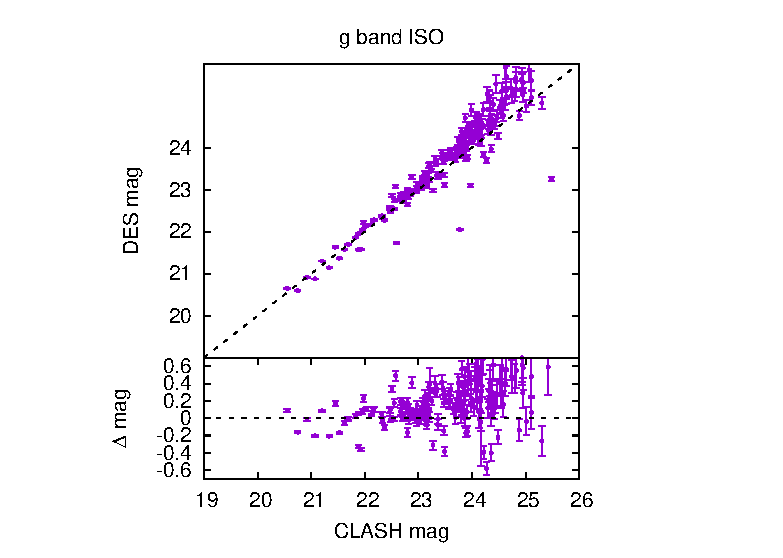
\includegraphics[width=0.6\textwidth]{/Users/apalmese/work/PhD_thesis/thesis_format/chapters/chapter4/Figures/delta_g_iso.eps}\hskip -1cm 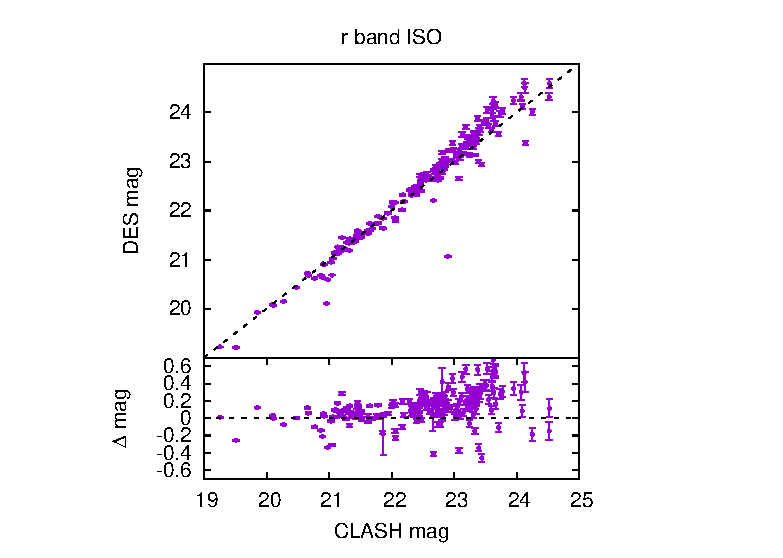
\includegraphics[width=0.6\textwidth]{/Users/apalmese/work/PhD_thesis/thesis_format/chapters/chapter4/Figures/delta_r_iso.eps}
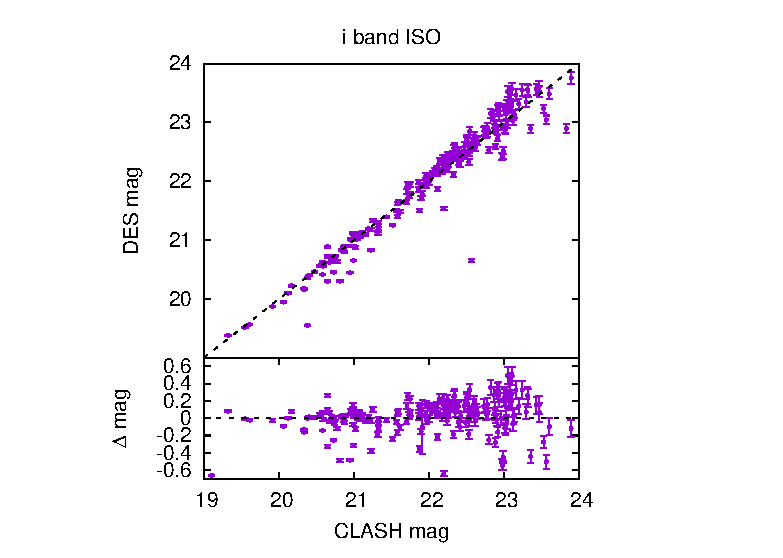
\includegraphics[width=0.6\textwidth]{/Users/apalmese/work/PhD_thesis/thesis_format/chapters/chapter4/Figures/delta_i_iso.eps}\hskip -1cm 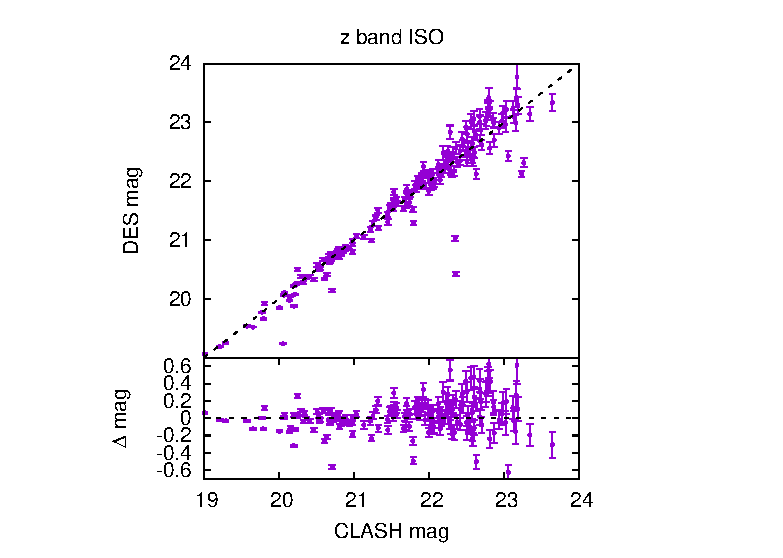
\includegraphics[width=0.6\textwidth]{/Users/apalmese/work/PhD_thesis/thesis_format/chapters/chapter4/Figures/delta_z_iso.eps}
\begin{center}
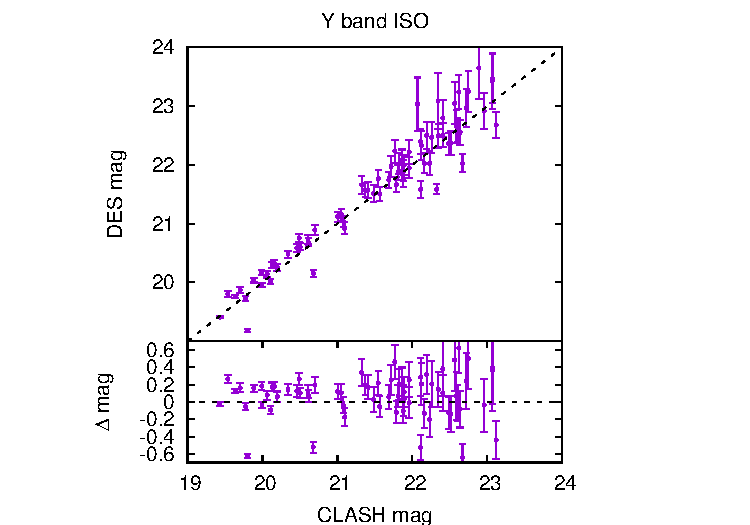
\includegraphics[width=0.6\textwidth]{/Users/apalmese/work/PhD_thesis/thesis_format/chapters/chapter4/Figures/delta_y_iso.eps}\end{center}
\caption{ DES magnitues compared to CLASH magnitudes, with bottom plots of $\Delta_{\rm m} =  m_{\rm CLASH} - m_{\rm DES}$ in the $g$,$r$,$i$ and $z$ bands for the matched sources that satisfy $S/N>10$ and filtering the sources with \texttt{FLAGS}$> 3$. CLASH errorbars are not plotted for visualisation purposes, while those on the DES magnitudes represent the $1\sigma$ error. The dashed black lines represent the ideal case $m_{\rm CLASH} = m_{\rm DES}$. }\label{deltamag}
\end{figure}
Considering only those matched sources with a signal to noise ratio $S/N>10$ in the DES $i$-band, excluding stars and objects with SExtractor $\texttt{FLAGS} > 3$ (in order to exclude objects with saturated pixels or corrupted data, but include objects that were initially blended) we are left with 327 sources observed in the $g$ and $r$ bands, and 331 in the $i$ and $z$ bands. The differences $\Delta_{\rm m} =  m_{\rm DES}- m_{\rm CLASH}$ are plotted in Figure \ref{deltamag}, as well as the DES magnitudes as a function of the CLASH ones for the matched sources. The magnitudes plotted are SExtractor isophotal magnitudes \texttt{MAG\_ISO} for both DES and CLASH. $\Delta_{\rm m}$ in the $griz$ bands has been corrected for the magnitude shifts due to the differences between these DES and HST filters. The offsets have been computed using two ``extreme case'' SED templates (one elliptical, one irregular) at the cluster redshift. We have not taken into consideration the $Y$ band offset as the HST and DES filters are too different, but we still report the comparison for completeness.

Figure \ref{deltamag} shows an offset in the DES magnitudes, especially in the $gri$ bands, which may be due to different choices of threshold or background when running SExtractor. Nevertheless the linear trend is clear, bringing to Pearson coefficients between 0.91 and 0.98 in all bands. The higher scatter that we could expect in the $Y$ band (as the corresponding CLASH filter is the F105W, which is much more spread towards the infrared than the DES $Y$ filter) is actually compensated for by higher DES photometric errors. The mean difference in magnitude $\Delta_{\rm m}$ between the two datasets is 0.13, 0.04, -0.07, -0.07 and 0.08 in the $grizY$ bands respectively.

\subsection{Star/galaxy separation}

For the purpose of studying the star/galaxy separation, we adopt the same notation used in \citet{soumagnac}. We study the galaxy completeness $c_g$, defined as the ratio of the number of true galaxies classified as galaxies to the total number of true galaxies (including then also the number of true galaxies classified as stars $M_G$):
\begin{equation}
c_g=\frac{N_G}{N_G+M_G}\;,
\end{equation}
where here $N_G$ is given by the galaxies in the DES catalogue, and the number of true galaxies is given by the object classified as such in CLASH.\\
Moreover the galaxy purity $p_g$ is defined as
\begin{equation}
p_g=\frac{N_G}{N_G+M_S}\;,
\end{equation}
where $M_S$ is the number of stars classified as galaxies.

We consider as true galaxies the sources that have a \textsc{SExtractor} stellarity index \texttt{CLASS\_STAR}$<0.08$ in the CLASH catalogue, otherwise they are stars. This cut has been proven to perform well in other CLASH works (e.g. \citealt{jouvel}). We try to understand if the star/galaxy performance is compatible between the two datasets.\\  

\begin{table}\centering
\begin{tabular}{c|cccc}
$\texttt{CLASS\_STAR}$&$g$&$r$&$i$&$z$\\
\hline
 $ G({\rm DES})$&    551&      538&      535&      522\\
  $G({\rm CLASH})$ &   553 &      553&      553   &   553\\
   $S({\rm  DES})$&  58 &      71&      74&      87\\
   $S({\rm CLASH})$& 56&      56&      56&      56\\
\end{tabular}\hskip 0.3cm
\begin{tabular}{c|cccc}
 $\texttt{SPREAD\_MODEL}$&$g$&$r$&$i$&$z$\\
\hline
 $ G({\rm DES})$&    388&      463&      428&      405\\
 $G({\rm CLASH})$ &   553 &      553&      553   &   553\\
   $S({\rm DES})$&  221 &      146&     181&      204\\
  $S({\rm CLASH})$& 56&      56&      56&      56\\
\end{tabular}\caption{Number of galaxies $G$ and stars $S$ found in DES and CLASH, when considering $\texttt{CLASS\_STAR}<0.8$ (top table) and $\texttt{SPREAD\_MODEL}>0.003$ (bottom table) for galaxies in DES.}\label{numbergal}
\end{table}
\begin{figure}
\vspace{ -0.5cm}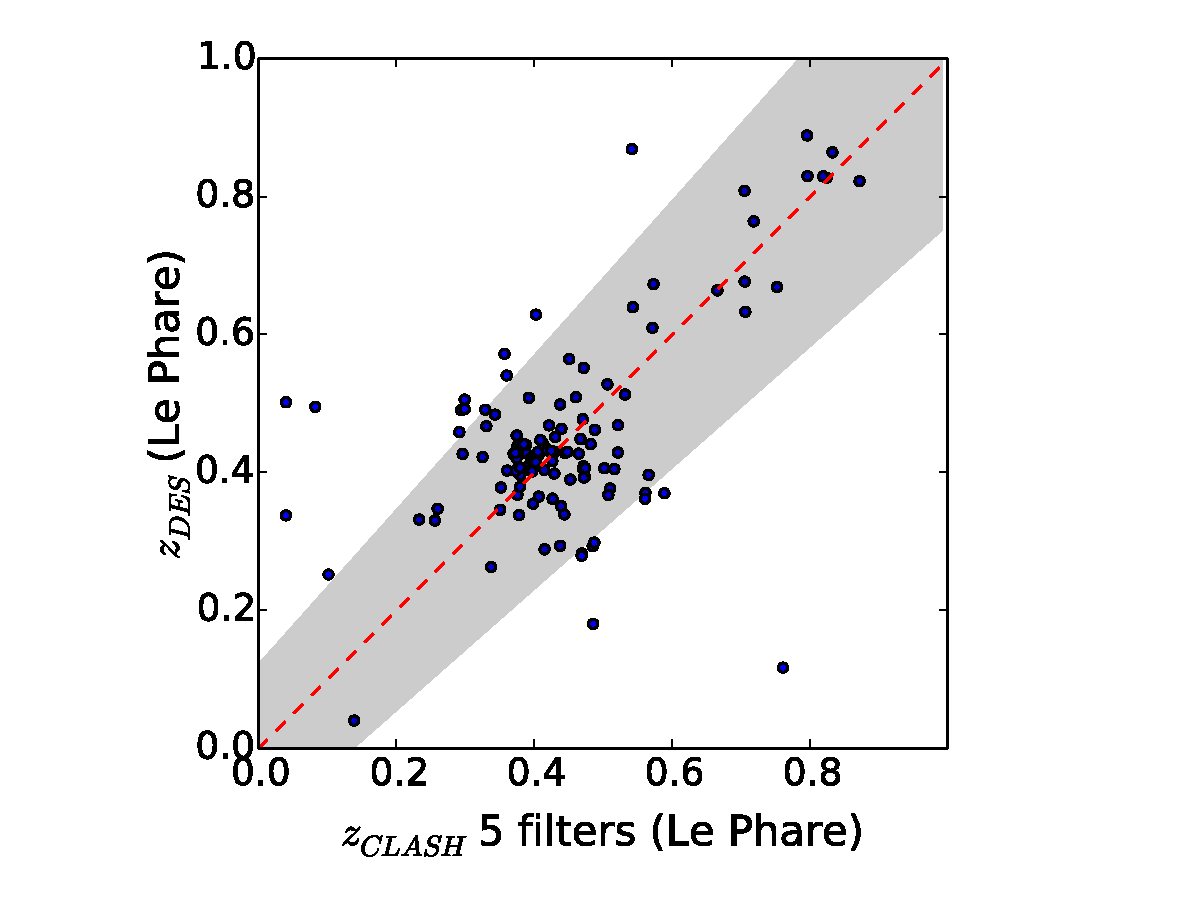
\includegraphics[width=0.37\textwidth]{/Users/apalmese/work/PhD_thesis/thesis_format/chapters/chapter4/Figures/des_vs_clash_5filt.pdf} \hspace{-0.1cm}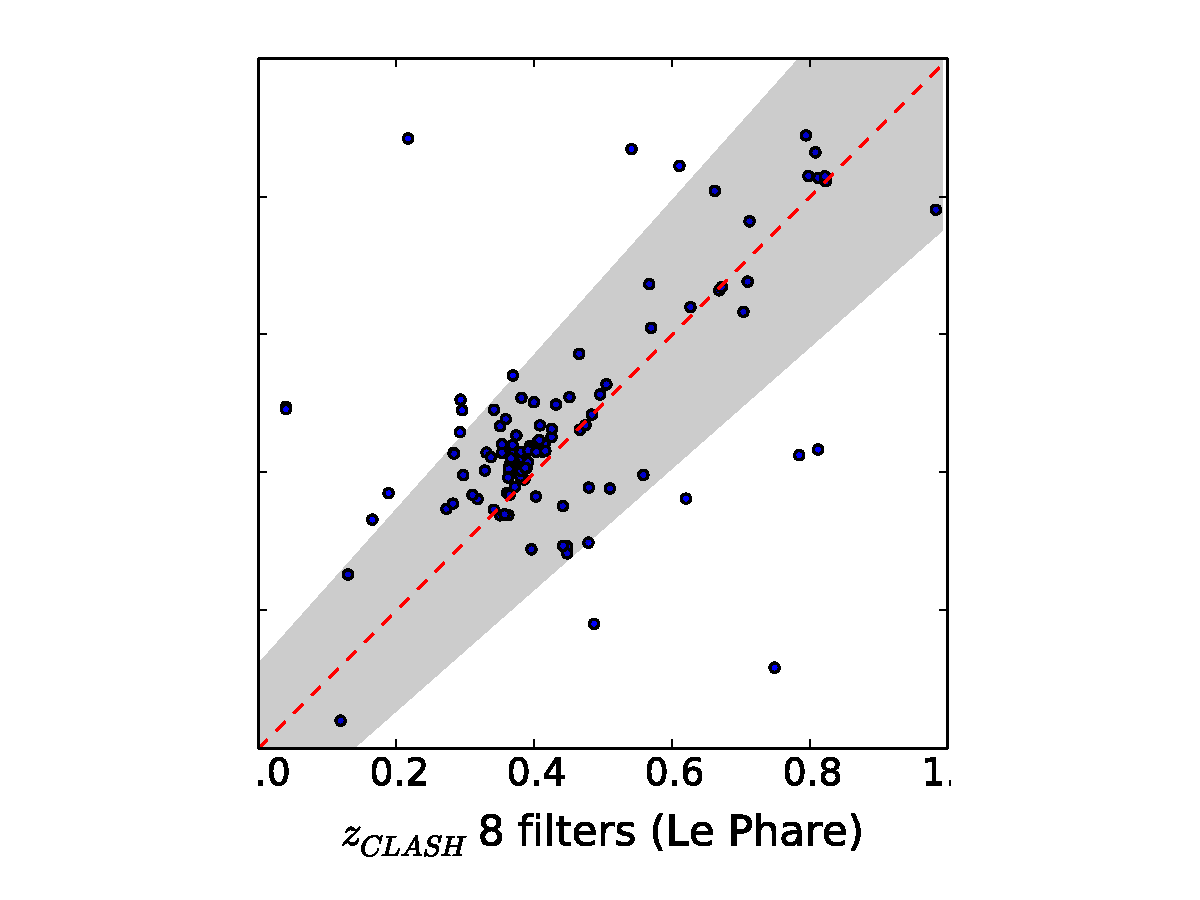
\includegraphics[width=0.3\textwidth]{/Users/apalmese/work/PhD_thesis/thesis_format/chapters/chapter4/Figures/des_vs_clash_8filt_1.pdf} \hspace{-0.22cm} 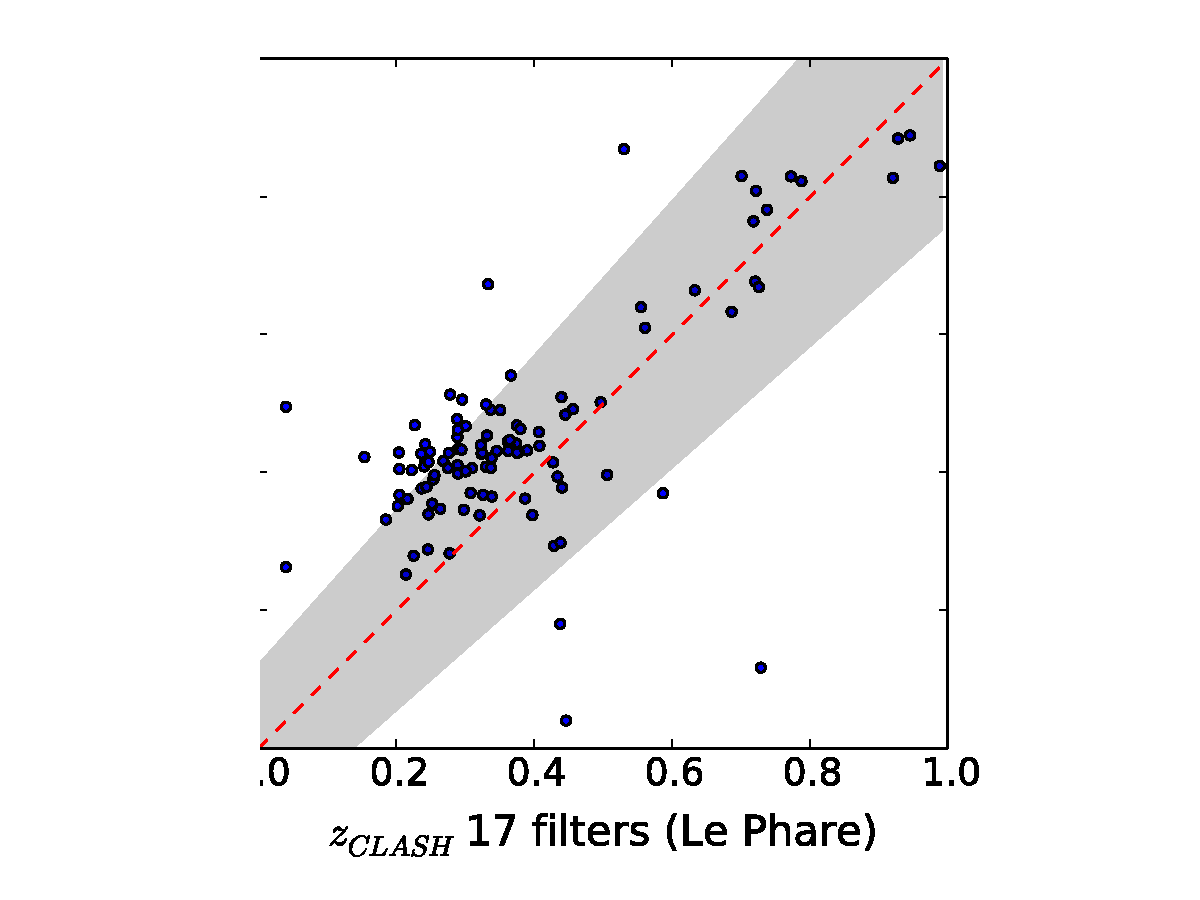
\includegraphics[width=0.308\textwidth]{/Users/apalmese/work/PhD_thesis/thesis_format/chapters/chapter4/Figures/des_vs_clash_17filt_1.pdf}
\caption{Comparison of the DES versus CLASH photo-$z$'s for the sources matched between the two catalogues. photo-$z$'s were obtained using \textsc{LePhare}. \emph{Top:} only the 5 HST filters similar to the $grizY$ filters in DES have been used to compute CLASH photo-$z$'s. \emph{Middle:} 3 of the HST UV filters have been added to the 5 HST optical filters for the CLASH photo-$z$ estimation. \emph{Bottom:} all the 17 available CLASH filters have been used to estimate the photo-$z$'s. The red dashed line represents $z_{DES}=z_{CLASH}$, and the grey area the expected DES accuracy of $|z_{DES}-z_{CLASH}|< \sigma(1+z_{CLASH})$, where $\sigma=0.12$.}\label{photoz}
\end{figure}

We first consider the \texttt{CLASS\_STAR} parameter given in the DES catalogue. We find that a cut between 0.7 and 0.9 for the \texttt{CLASS\_STAR\_I} gives purity and completeness above the 90\%. The number of galaxies and stars in the two catalogues can be found in Table \ref{numbergal}.

We also test the performance of star/galaxy separation with the \texttt{SPREAD\_MODEL} parameter (defined in \citealt{desai} and tested in \citealt{spreadmodel}). \texttt{SPREAD\_MODEL}  is a morphological star/galaxy separation parameter given by \textsc{SExtractor} which acts as a linear discriminant between the best fitting local PSF model and a slightly ``fuzzier'' version made from the same PSF model, convolved with a circular exponential model. A threshold is set to 0.003 by the DESDM pipeline to separate stars (PSF like, having absolute values below 0.003) from galaxies (non-PSF like, with values higher than 0.003). As a result, 77.4\% of the galaxies are catalogued in DES as such, and the purity is 97.3\%. 
 A plot for the purity and the completeness for varying  $\texttt{SPREAD\_MODEL\_I}$ cuts is shown in Figure \ref{purity}. We list the number of galaxies and stars in the two catalogues in Table \ref{numbergal}. It can be seen from Figure \ref{purity} that cut at lower values ($\sim 0.001-0.002$) would give a higher completeness without affecting the purity significantly. Moreover, in this case may be better using the $\texttt{SPREAD\_MODEL}$ in the $r$ band, which is deeper than the $i$ one, and this can also be seen in Figure \ref{purity}, where it is clear that, for the same cut, the completeness is higher. We also find that using the \texttt{CLASS\_STAR} parameters with the mentioned cut is more efficient than adopting the \texttt{SPREAD\_MODEL\_I} with the cut at 0.003.

\subsection{Photo-$z$}\label{sec:z}
Considering only those matched sources with a signal to noise ratio $S/N>10$ in the DES $i$-band, excluding stars (in this case we exclude all objects with \texttt{CLASS\_STAR\_I}$>0.8$) and objects with $\texttt{FLAGS}\neq 0$ (in order to exclude objects with saturated pixels or corrupted data, and originally blended sources) we are left with 155 sources. This is the subset of galaxies that we will use for the photo-$z$ and stellar mass comparison.

In order to estimate the photo-$z$'s, we used the publicly available software \lephare (\citealt{arnouts}, \citealt{ilbertlephare})\footnote{\url{http://www.cfht.hawaii.edu/~arnouts/LEPHARE/lephare.html}}, as it also produces the stellar masses that we want to study in this work. Previous works on DES photo-$z$'s have tested the performance of this code in comparison with other softwares and spectroscopic redshifts. In particular, \citet{sanchez} found that \lephare fulfils the DES requirements on scatter and $2\sigma$ outlier fraction when it is run on SV data, and the metrics obtained are compatible with those from other template-based methods within 10\%. Training-based methods showed a lower bias compared to template-fitting codes, and this can be improved in the latter using adaptive recalibration methods, which are available in \textsc{LePhare}. However, stellar masses tests have not been performed with DES data so far.

We therefore need to further check the DES photo-$z$ and stellar mass estimation with \lephare first. This is where the HST data are particularly useful in this work, as we need to check DES against a more precise photometric survey covering the wavelengths from optical to IR. 

Furthermore, \lephare is a reliable code, as seen in e.g. \citet{cosmos}.

\subsubsection{Results}
We run \lephare on both CLASH (with 5, 8 and all 17 filters) and DES (5 filters) catalogues, fitting the 31 synthetic SEDs templates given by the COSMOS (see \citealt{cosmos}) libraries. We use four galaxy extinction values ranging from 0.05 to 0.3 using a \citet{calzetti} extinction law for DES. For CLASH, two more extinction values are added (0.4 and 0.5), in order to take into account the wider wavelength range covered when we use all its filters. 

The results are plotted in the upper panel of Figure \ref{photoz} for the 155 matched sources when 5 filters are considered for CLASH. 
 Of all the sources considered, 85\% have a photo-$z$ which is compatible with the CLASH photo-$z$ within the DES requirement\footnote{Where $z_p$ and $z_s$ are the photometric and spectroscopic redshifts, so here we consider the CLASH photo-$z$ as the ``spectroscopic'' one. } $|z_{p}-z_{s}|< \sigma(1+z_{s})$, where $\sigma=0.12$. 
We notice an offset in the CLASH redshift when 17 filters are used (see lower panel of Figure \ref{photoz}), while 77\% of the sources still satisfies the DES requirement. This most likely stems from the inclusion of near-UV filters to get an accurate redshift from the Balmer break for galaxies below a redshift of 0.4 (see e.g. \citealt{Eisenstein2}). In fact, this offset starts to be seen also when adding only three UV bands (namely F336W, F390W and F435W) to the $grizY$ filters (see middle panel in Figure \ref{photoz}). A problem around redshift 0.4 for DES galaxies had already been seen in \citet{sanchez} (see their Figure 5) and \citet{bonnett}. In particular, \citet{bonnett} also pointed out a lack of matching SEDs for galaxies around redshift 0.4 with template fitting methods (see their Figure 8). 

Zero points\footnote{Zero--points define the shift in the observed magnitudes due to various systematics.} have not been adopted in the DES photo-$z$ estimation, as we saw that their introduction causes systematic effects. Zero points are calculated using field galaxies, so we believe we would need spectroscopy in the cluster field to be helpful at photo-$z$ calibrations for this study.\\

\subsection{Stellar Masses}\label{clash_sm}

Stellar masses are key observables in the study of galaxy evolutionary models. Unfortunately, they cannot be directly measured, but require multicolour photometry to be fitted with stellar population models, therefore making a series of assumptions. One of these is the galaxy redshift if spectroscopy is not available: in the view of our goal of computing the stellar mass profile of the RXJ2248 cluster, we have to bear in mind that galaxy redshift accuracy is essential not only to ensure the correct template match in the template fitting method here used and the distance to the galaxy, but also to determine the cluster membership. We will therefore see how the redshift assumptions affect the stellar mass estimation and elaborate a reasonable technique to correctly estimate the stellar mass profile.

\subsubsection{Method}
We use the same sample of matched galaxies with $S/N>10$ used in Section \ref{sec:z} and their redshift estimations in order to compute the stellar masses for both DES and CLASH using \textsc{LePhare}. In the first place, the redshifts of the galaxies are fixed to those photo-$z$'s previously computed ($i.e.$ to DES photo-$z$'s for DES stellar masses, and to CLASH photo-$z$'s for CLASH stellar masses). In the second case, we fix the galaxy redshifts at the cluster redshift for both DES and CLASH, and the \textsc{LePhare} DES photo-$z$'s are only used to select a subsample of cluster members satisfying $|z_{phot}-z_{cl}| \le 0.12$. For this subsample both DES and CLASH stellar masses are estimated.

 We chose to use \textsc{LePhare}, together with the \citet{bc03} templates, as this combination has been shown to be robust in the estimation of physical parameters of galaxies (\citealt{ilbert2010}).

We derive our stellar mass estimates by fitting synthetic SEDs templates while keeping the redshift fixed as described previously in the two cases. The SED templates are based on the stellar population synthesis (SPS) package developed by \citealt{bc03} (BC03) assuming a \citet{chabrier} initial mass function (IMF). Our initial set of templates includes 9 models using one metallicity ($Z=1 Z_\odot$) 
and nine exponentially decreasing star formation rates $\propto exp(-t/\tau)$ where $t$ is the time and $\tau$ takes the values $\tau = 0.1,0.3,1,2,3,5,10,15,30$ Gyr. The final template set is then generated over 57 starburst ages ranging from 0.01 to 13.5 Gyr, and four extinction values ranging from 0.05 to 0.3 using a \citet{calzetti} extinction law. For CLASH, two more extinction values are added (0.4 and 0.5).

The uncertainties on our stellar masses estimates (\texttt{MASS\_BEST} from \textsc{LePhare}) are given by the 68\% confidence limits on the SED fit.
\begin{figure}\centering
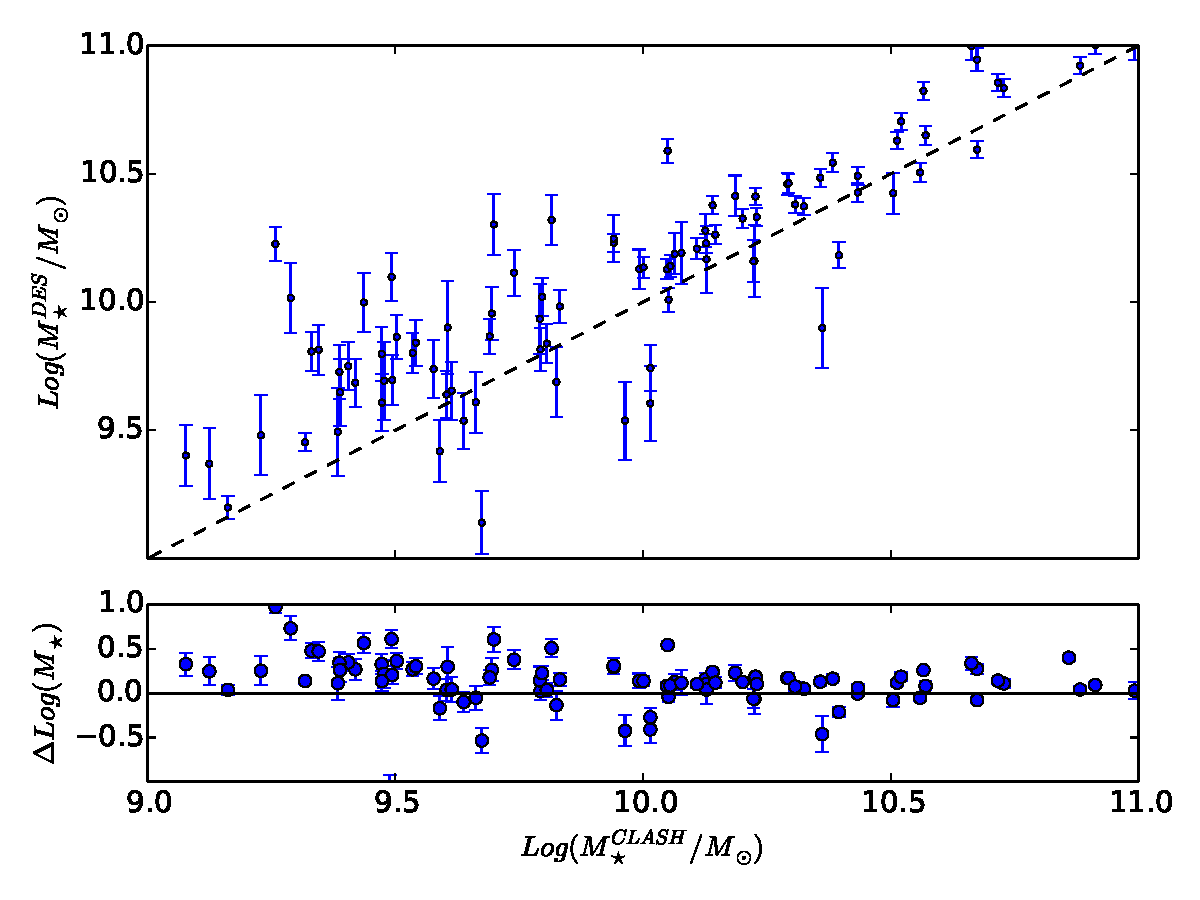
\includegraphics[width=0.7\textwidth]{/Users/apalmese/work/PhD_thesis/thesis_format/chapters/chapter4/Figures/clashvsdes.pdf}
\caption{DES stellar masses versus CLASH stellar masses computed using \textsc{LePhare}. In the stellar mass estimation, each source is  assumed to be at the redshift given as output by \textsc{LePhare}, as described in Section \ref{sec:z}. The dashed line line represents $M_\star^{DES}=M_\star^{CLASH}$. In the bottom panel $\Delta Log(M_\star)=Log(M_\star^{DES})-Log(M_\star^{CLASH})$ is presented. All available filters (\emph{i.e.} 5 for DES and 17 for CLASH) have been used in the estimation process. Uncertainties represent the 68\% Confidence Level.}\label{SMdesvsclash}
\end{figure}
\begin{figure}\centering
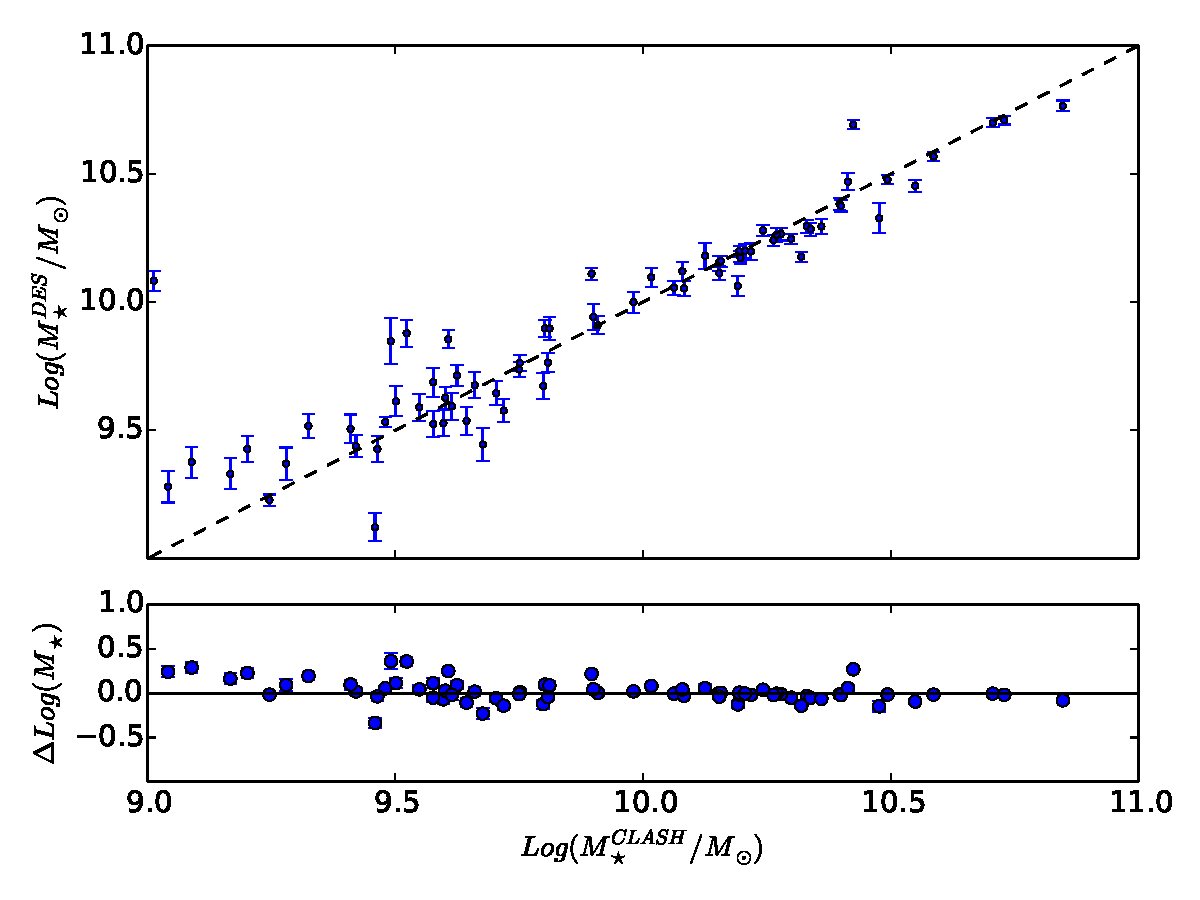
\includegraphics[width=0.7\textwidth]{/Users/apalmese/work/PhD_thesis/thesis_format/chapters/chapter4/Figures/clashvsdes_zcl.pdf}
\caption{DES stellar masses versus CLASH stellar masses computed using \textsc{LePhare}. Here only sources around the cluster redshift are considered (\emph{i.e.} sources with a DES photo-$z$ that satisfies $|z-z_{cl}| \le 0.12$, where $z_{cl}=0.3475$ is the cluster redshift). In the DES and CLASH stellar mass estimation, these galaxies are all assumed to be at $z_{cl}$. The dashed line line represents $M_\star^{DES}=M_\star^{CLASH}$. In the bottom panel $\Delta Log(M_\star)=Log(M_\star^{DES})-Log(M_\star^{CLASH})$ is presented. The offset seen in Figure \ref{SMdesvsclash} seems to disappear in this plot, showing that this effect was due to the photo-$z$ offset. All available filters (\emph{i.e.} 5 for DES and 17 for CLASH) have been used in the estimation process. Uncertainties represent the 68\% Confidence Level.}\label{SMdesvsclash_zcl}
\end{figure}
\begin{figure}\centering
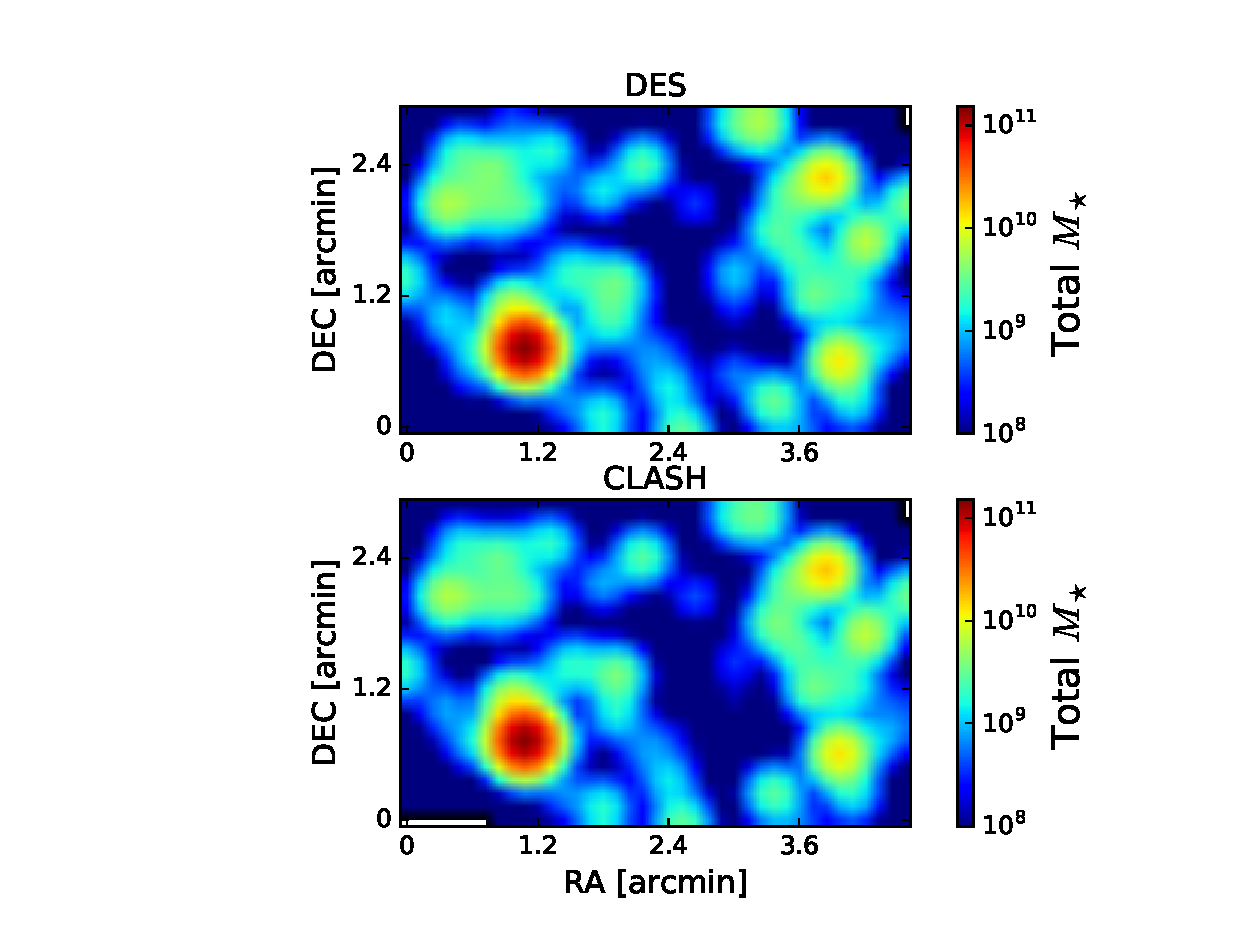
\includegraphics[width=0.7\textwidth]{/Users/apalmese/work/PhD_thesis/thesis_format/chapters/chapter4/Figures/maps_des_and_clash.eps}\caption{DES and CLASH total stellar mass maps computed using \lephare for the galaxies matched between the two catalogues. The stellar masses plotted are the same as those shown in the bottom panel of Figure \protect\ref{SMdesvsclash_zcl} (\emph{i.e.} all the galaxies with a DES photo-$z$ that satisfies $|z-z_{cl}| \le 0.12$, where $z_{cl}$ is the cluster redshift, have a redshift fixed to $z_{cl}$ in the SED fitting). The map is centred on the BCG, but its stellar mass is not visible as it was originally blended and therefore did not pass the quality flag cut applied in Section \ref{clash_sm}. The resolution is $0.12'/$pixel and the map is smoothed with a Gaussian of $\sigma=0.144$ arcmin. At the cluster redshift, $1'$ corresponds to 294 kpc in the assumed cosmology.}\label{desclashmaps}
\end{figure}

\subsubsection{Photo-$z$ consistency test}\label{test}
In this Section we test whether the fact that we assumed a photo-$z$ that was computed with a certain set of templates to then compute the stellar mass with a larger set of templates is consistent. With photometric surveys data, it is a common method to perform estimation of the photometric redshift and SED fitting in two steps, which involve fixing the redshift of a galaxy at the best fit value obtained in the first step. Although this may not be the most elegant way of solving the problem of the lack of spectroscopic information, it has been proven to lead to only a small bias in the SED fitting parameters, when compared to results given by the simultaneous estimation of redshift and stellar mass (see \citealt{acquaviva}). Moreover, here we can take advantage of the prior information that this is a cluster.

In order to do test the consistency of the photo-$z$ choice, we want to show that the resulting photo-$z$ is not drastically dependent on the choice of templates. Therefore, we compare the photo-$z$'s given by Le Phare when using the COSMOS templates and the BC03 ones. A comparison is shown in Figure \ref{bc03vscosmos} for all the galaxies in the DES field of view. We retrieve that $71\%$ of the galaxies have $|\Delta z|=|z_{BC03}-z_{COSMOS}|<0.12$.
\begin{figure}
\includegraphics[width=0.5\textwidth]{/Users/apalmese/work/PhD_thesis/thesis_format/chapters/chapter4/Figures/bc03_vs_cosmos_density.eps}
\includegraphics[width=0.5\textwidth]{/Users/apalmese/work/PhD_thesis/thesis_format/chapters/chapter4/Figures/delta_cosmos_bc03.eps}\caption{\emph{Left panel}: Comparison  of the photo-$z$'s computed using the Bruzual and Charlot 2003 templates and those using the COSMOS templates. \emph{Right panel:} Residuals of the photo-$z$'s computed using the two differnt set of templates.}\label{bc03vscosmos}
\end{figure}


\begin{figure}
\centering
\includegraphics[width=0.48\textwidth]{/Users/apalmese/work/PhD_thesis/thesis_format/chapters/chapter4/Figures/p_g_spread_r.eps}
\includegraphics[width=0.48\textwidth]{/Users/apalmese/work/PhD_thesis/thesis_format/chapters/chapter4/Figures/p_g_spread_i.eps}
\caption{Galaxy purity (blue dashed line) and completeness (black solid line) for the star/galaxy separation problem using the \texttt{SPREAD\_MODEL} parameter in the DES catalogue for the $r$ (top) and $i$ (bottom) bands. The red vertical line represents a typical cut used for \texttt{SPREAD\_MODEL}, which is  0.003.}\label{purity}
\end{figure}



\subsubsection{Results}
 In Figure \ref{SMdesvsclash}, we show the comparison between DES and CLASH stellar mass estimates for the first case, where the redshifts are fixed to the \textsc{LePhare} estimates.
 The linear correlation between the two estimates is clear, but there is an offset of mean value $\sim 0.16$ dex. This should be considered in light of two aspects:
\begin{enumerate}
\item the offset in the photo-$z$'s that we addressed in Section \ref{sec:z};
\item the uncertainties in the DES stellar masses may be underestimated as those are the 68\% confidence limits on the SED fit and do not take into account systematic error contribution.
\end{enumerate}

In Figure \ref{SMdesvsclash_zcl} we show the results for the second case, where we select the galaxies with a DES photo-$z$ close to the spectroscopic cluster redshift $z_{cl}$, satisfying $z_{cl}-0.12<z_{phot}<z_{cl}+0.12$. The redshift of these sources is fixed at $z_{cl}$ in the stellar mass estimation, and the reason for this choice is twofold:
\begin{enumerate}
\item to minimise circularity associated with using \textsc{Le Phare} to both measure redshifts and stellar masses;
\item to take into account the shift in the redshift estimates pointed out in Section \ref{sec:z} (and therefore put at the correct cluster redshift the cluster members which photo-$z$ appeared to be at $z_{phot}\sim 0.4$).
\end{enumerate}

Of course this choice results in considering some sources as being at $z_{cl}$ even though they are not, and we shall take this into account in the following.  A consistency test for the choice of redshifts done is presented in Appendix \ref{test}.

The correlation between the estimated stellar masses significantly increases if also the CLASH sources are set to be at the cluster redshift, as seen in a comparison of Figure \ref{SMdesvsclash} with Figure \ref{SMdesvsclash_zcl}, where we find that stellar masses from DES can be estimated within 25\% of CLASH values. This shows that the offset seen in the former is due to the offset in the redshifts given in input, rather than other systematics. Therefore, the wavelengths covered by the DES broadband filters are capable of providing a good estimation of stellar mass if the photometric redshift is sufficiently precise. 

In Figure \ref{desclashmaps} we show the spatial distribution of the total stellar mass spatial distributions for both DES and CLASH in the CLASH field ($\sim 4.8'\times 4.2'$), represented with a resolution of $0.12'/$pixel and smoothed with a Gaussian of $\sigma=0.144$ arcmin. The stellar masses of galaxies are summed over in each pixel.
Obviously the two samples show very good agreement in terms of the spatial distribution of stellar mass. The Pearson coefficient for the pixel by pixel stellar mass values of the two non-smoothed maps is 0.93. The difference map without any smoothing has a mean of 0.02 and $\sigma=0.12$.

\section{Dark Matter and Stellar Masses}\label{DMandSM}
In this section we study the stellar mass radial profile of the cluster and relate it to that of dark matter that has been obtained though DES weak lensing studies in \citet{melchior}. As shown in Section \ref{clash_sm}, stellar mass estimation can be biased if the redshift assumed is biased too: this is a problem if one wants to compute stellar masses with photometric surveys data. In the lack of spectroscopy, it is a common method to perform estimation of the photometric redshift and SED fitting in two steps, which involve fixing the redshift of a galaxy at the best fit value obtained in the first step. Although this may not be the most elegant way of solving the problem, it has been proven to lead to only a small bias in the SED fitting parameters, when compared to results given by the simultaneous estimation of redshift and stellar mass (see \citealt{acquaviva}). Nevertheless, here we want to adopt a more consistent methodology for the stellar mass estimation, taking advantage of the fact that we are looking at a cluster with a known redshift. This technique is outlined in the first part of this section, followed by a study of the different mass radial profiles obtained. To allow a straightforward comparison with the weak lensing reconstructed mass, we compute total stellar mass and surface density on a projected 2-dimensional plane, \emph{i.e.}:
\begin{equation}
M_\star(R)=\sum_i m_\star^i \qquad\Sigma_\star(R)=\frac{\sum_i m_\star^i}{A_\mathrm{annulus}}\, ,
\end{equation}
where the sums are intended over the galaxies within annuli of projected radius $R$. Similar definitions apply for the cumulative distributions $M_\star(<R)$ and $\Sigma_\star(<R)$, computed within circles of radius $R$.  The centre of the image is taken to be that of the BCG. At last, we present a comparison between the stellar and total DES mass maps.


\subsection{Galaxy samples and stellar mass estimates}   
Our goal is to compare the reconstructed mass from weak lensing to the total stellar mass of the cluster members. In order to do so, we split the galaxies into two populations. The following steps are performed:
\begin{itemize}
\item We select the red members using the \textsc{RedMaPPer} SV catalogue (\citealt{rykoff}), which identifies cluster members with high precision (\citealt{rozo}). Their stellar masses are computed using the same parameters presented in Section \ref{clash_sm} (but fixing the redshift at $z_{cl}$). 
\item The \textsc{RedMaPPer} galaxies profile has been corrected by a factor representing the contribution coming from faint sources at luminosities smaller than the limit of the sample (0.2$L^*$). This is done by integrating the luminosity with a Schechter function, \emph{i.e.} we computed the fraction:
\begin{equation}
F_L=\frac{\int^{0.2L^*}_0 L \phi(L)d L }{\int_{0}^\infty L\phi(L)d L} \, ,
\end{equation}
where $\phi(L)=\phi_*(\frac{L}{L^*})^\alpha e^{-L/L^*}$ with $\alpha =-1$ (as done in \citealt{redpaper} for the SDSS sample, that has properties similar to DES). We find that the galaxies below the luminosity limit contribute to a fraction $F_L=0.18$ of the total luminosity, and therefore, assuming a constant $M_\star/L$ ratio for the red galaxy population, they contribute to the same percentage of stellar mass.
\item The contribution to the total stellar mass of each red member is weighted by its membership probability (reported in the RedMaPPer catalogue).
\item In order to study the mass profile at radii higher than $r_{200c}$, we decide not to neglect the contribution coming from the bluer population. First, we exclude all objects with saturated pixels or corrupted data, but include galaxies that were initially blended (such as the BCG). Then we select the rest of the galaxies in the field of view that have magnitudes $m_i$ in the $i$ band satisfying $m_i^\mathrm{BCG}<m_i<m_i^\mathrm{lim}$. In this way we exclude any source which is brighter than the BCG and cut at $m_i^\mathrm{lim}=21$ mag in order to ensure the completeness of the sample. After having performed a SED fitting as in the previous step, we filter out all galaxies that do not give a good fit (cutting on reduced $\chi^2<2$) when the redshift is fixed at the cluster value. 
\end{itemize}


\subsection{Masking and background correction}

We estimate the survey area lost due to masked regions and blending of faint galaxies with large cluster members near the core. We calculate corrections for both effects as follows.
\begin{itemize}
\item \textsc{Healpix} \citep{healpix} maps of depth and masking fractions are produced for DES with \textsc{Mangle}
\citep{mangle}. From these, we calculate mean depth and fractions of masked area in our set of annuli. The depth is approximately constant out to $\approx 50$ arcmin from the BCG, which defines the outer limit of the area used for our background estimation scheme. Masking fractions are below 5 per cent for all annuli and applied to the binned stellar mass estimates from both galaxy samples.
\item For the blue galaxy sample, some objects are lost due to blending with cluster member galaxies. Without correction, this would bias our stellar mass estimates of blue galaxies near the cluster centre low. We estimate the area lost in each annulus as the isophotal area above the \textsc{SExtractor} detection threshold,
\texttt{ISOAREA\_I}. This yields a $\approx 7$ per cent correction in the innermost arcminute, which drops quickly towards larger radii. For the blue galaxy sample, this correction and the masking fraction are applied in an additive fashion.
\end{itemize}

The contribution coming from galaxies that do not actually sit at the cluster redshift is removed from the blue galaxies sample by performing a background subtraction: we estimate the projected surface density of the stellar mass $\Sigma_\star(R)$ at large radii ($30-50$ arcmin, which means outside $\approx 4r_{200c}$ \footnote{$r_{200c}=2200$ kpc from the NFW fit of \citet{melchior}, which means $r_{200c}\simeq7.46'$ at the cluster redshift}), where the stellar mass profile tends to become flat. The value found is $\Sigma_\star=1.36\times 10^{10} M_\odot/\textrm{arcmin}^2$ and this is subtracted on the smaller scales, with an uncertainty given by a Poissonian error. The remaining stellar mass contribution is then added to that of the red galaxies. 


\subsection{Stellar mass profile}

\begin{figure*}
\includegraphics[width=1\textwidth]{/Users/apalmese/work/PhD_thesis/thesis_format/chapters/chapter4/Figures/all_profiles.png}
\caption{Cumulative radial distributions of total stellar mass for the DES red (red points), blue (blue points) and all galaxies (purple points) in the cluster, together with the total, non-parametric mass profile reconstructed from DES weak lensing (\citealt{melchior}, green points). The purple solid line is our NFW fit to the DES stellar mass profile, while the blue solid line is the NFW best fit from DES weak lensing. The black points represent the CLASH total stellar mass profile computed in this work, with our NFW fit (black solid line). The red solid line is the \citet{umetsu15} NFW best-fit for CLASH from a strong lensing, weak lensing and magnification joint analysis. This profile is restricted to the NFW fitting range $R<2 {\rm Mpc }\; h^{-1}$ chosen in \citet{umetsu15}, which is larger than the HST field of view as other datasets were used in a joint analysis. The radius $R$ is projected, and $r_{200c}=2.2$ Mpc. Errorbars show the 68\% confidence level. }\label{sm_profile}
\end{figure*}

We look at the radial distribution of stellar mass, taking into account both the red cluster members present in the \textsc{RedMaPPer} catalogue, and the blue members, as explained in the previous section. The splitting into red and blue galaxies is justified by the possibility of improving the SED fitting by using different priors for the two populations, and considering the systematics differently. In fact, it is well known that stellar masses estimated for quiescent galaxies are more reliable than for star-forming ones, partially because the colour--$M_\star/L$ (from which $M_\star$ is derived) relation are more uncertain for very blue colours (see e.g. \citealt{conroy} and \citealt{banerji}).

The total stellar mass cumulative profiles $M_\star(<R)$ for the red and blue galaxies are shown in Figure \ref{sm_profile}. Within the innermost 5 arcmin, the contribution of the red cluster members to the total stellar mass is dominant ($\gtrsim 80\%$) with respect to the bluer galaxies, while at larger radii, namely outside $r_{200c}$, the second population considered gives a $20\ldots 50\%$ contribution to the total stellar mass.
In Figure \ref{sm_profile} we also plot the stellar mass profile from CLASH, where the galaxy cluster members were selected cutting on the CLASH photometric redshift with $|z_{phot}-z_{cl}|<0.12$.
 
 \subsection{Comparison to total mass from Weak Lensing}
 
The weak lensing mass profile is computed through the aperture mass densitometry (see \citealt{clowe}) using $M_{tot}(<R)=\pi R^2\zeta(<R)\Sigma_{cr}(z_l,z_s)$, where $\zeta(<R)=\bar{\kappa}(<R)-\bar{\kappa}(r_1<r<r_{2})$ is the difference between the mean convergence within a circular aperture of radius $R$ and the mean convergence between $r_1$ and $r_2$ (annulus radii that are fixed for all the apertures in the measurement), $z_l$ and $z_s$ are the redshift of lens and sources.  The convergence $\kappa$ is defined as the projected surface mass density  $\Sigma$, in units of the critical surface mass density $\Sigma_c$:
\begin{equation}\centering
\kappa=\frac{\Sigma}{\Sigma_c}\, , \qquad \Sigma_c=\frac{c^2}{4\pi G}\frac{D_s}{D_d D_{ds}}\,
\end{equation}
where $D$ stands for angular diameter distance and the subscripts $s, d, ds$ indicate the distance from the observer to the source, from the observer to the lens, and from the lens to the source respectively. In particular, \citet{melchior} used $r_1=30$ arcmin and $r_{2}=45$ arcmin. This explains our choice of estimating the stellar mass surface density background in the range 30 to 50 arcmin, where its profile is also essentially flat.
In Figure \ref{sm_profile} we also present the NFW mass profile derived by using the best fit parameters as found in \citet{melchior} for this cluster.
Given the similarity between the WL and  stellar mass profiles, we try to fit the stellar mass one with a NFW projected mass profile, as  the one derived in e.g. \citet{nfwfit}:

\begin{equation}
M(<x) = \left\{ \begin{array}{ll}
\frac{3 \delta_c M_{200c}}{200 c_{200}^3}
\left[\frac{2}{\sqrt{1-x^2}}{\rm arctanh}\sqrt{\frac{1-x}{1+x}}+ {\rm ln}(\frac{x}{2})
 \right] & ({\rm if }\;x < 1)\\
 %\hspace{4.2cm} \mbox{$\left({\rm if }\;x < 1\right)$} &\\ 
 & \\
\frac{3 \delta_c M_{200c}}{200 c_{200}^3}\left[ 1+{\rm ln}(\frac{1}{2})
 \right]  & ({\rm if }\;x = 1) \\
 %  \hspace{4.2cm}\mbox{$\left({\rm if }\;x = 1\right)$}&\\ 
 & \\
\frac{3 \delta_c M_{200c}}{200 c_{200}^3}\left[\frac{2}{\sqrt{x^2-1}}{\rm arctan}\sqrt{\frac{x-1}{1+x}}+ {\rm ln}(\frac{x}{2}) \right]
& ({\rm if }\;x > 1)\\
 %\hspace{4.2cm} \mbox{$\left({\rm if }\;x > 1\right)$} &
\end{array}
\right.\label{2dmass}
\end{equation}
where $x=R/r_{s}$, $c_{200}=r_{200c}/r_s$ is the concentration parameter and 
\begin{equation}
\delta_c=\frac{200}{3}\frac{c_{200}^3}{{\rm ln}(1+c_{200})-c_{200}/(1+c_{200})}\,.
\end{equation}

Our non-linear least squares fit uses the Levenberg-Marquardt algorithm and gives the following parameters for DES stellar mass profile: $M_{200c}^\star= (5.38\pm 0.11)\times 10^{12} M_\odot$, $c_{200}^\star= 2.4  \pm 0.13 $ with a reduced $\chi ^2=0.6$.


\begin{figure}
\centering
\includegraphics[width=0.7\textwidth]{/Users/apalmese/work/PhD_thesis/thesis_format/chapters/chapter4/Figures/f_profiles.png}
\caption{Cumulative radial distribution of the fraction of stellar mass of the galaxies in the cluster as computed in this work over the total mass from lensing studies. For the DES $f_\star$, the total mass comes from the non-parametric reconstruction of the weak lensing shear profile done in \citealt{melchior} (purple points), or from their NFW best fit (green squares). For CLASH, $M_{tot}$ is a result of the \citet{umetsu15} NFW best-fit for CLASH from a strong lensing, weak lensing and magnification joint analysis (red triangles). The mean DES stellar mass fraction from non-parametric weak lensing mass profile is $f_\star=(7.3 \pm  1.7)\times10^{-3}$, and is represented by the dashed line. The radius $R$ is projected, and rescaled with $r_{200c}=2.2$ Mpc. Errorbars show the 68\% confidence level.}\label{f_profile}
\end{figure}

From the DES stellar mass profile and the aperture mass densitometry total matter profile, we derive the stellar mass fraction $f_\star (<R)=M_\star(<R)/M_{tot}(<R)$, which is represented by the purple points in Figure \ref{f_profile}. Within $r_{200c}$ radius, we find $f^{DES}_\star (<r_{200c})=(6.8\pm 1.7)\times10^{-3}$, compatible within 1$\sigma$ in the outer regions with the result from \citet{bahcall}: $f_\star \simeq (1.0 \pm 0.4)\times10^{-2}$ above $\sim 300 h^{-1}$ kpc. In their paper, \citet{bahcall} examine the stellar fraction profile by stacking $> 10^5$ SDSS groups and clusters, divided into 3 richness subsamples.\footnote{They define the richness $N_{200}$ as the number of galaxies in the red sequence with rest-frame $i$-band luminosity $L_i>0.4L^*$ located within a radius $r^{gals}_{200}$ from the BCG (i.e. within the radius where the local galaxy overdensity is 200).} Inside $r_{200c}$ we recover a lower stellar mass fraction compared to their work. The discrepancy can be explained in light of the different analyses carried out in \citet{bahcall}:
\begin{itemize}
\item \citet{bahcall} stack clusters with different properties and at different redshifts.
\item They included the contribution of the diffuse intracluster light (ICL), which increases $f_\star$ by a factor 1.15 within $r_{200c}$.
\item The luminosity profiles and weak lensing mass profiles have been de-projected to obtain 3D profiles in their work. On the other hand, considering the projected $f_\star$ means that we are including the contribution of the cluster outskirts along the line of sight when we look at cluster core. In these regions, the stellar mass fraction is lower, and this tends to reduce 2D $f_\star$ at small radii with respect the 3D behaviour.
\end{itemize}

 On the other hand, the average stellar mass of the Universe, estimated to be $f_{\star,cosmic}=(9\pm1)\times 10^{-3}$ (as derived in \citealt{bahcall}) is recovered outside $r_{200c}$, as we would expect even for a projected profile.
 
Overall, no particular radial trend is found, in agreement with \citet{bahcall} and also with \citet{andreon}, who studied the stellar-to-total mass ratio of three CLASH clusters at $z\sim 0.45$. Nevertheless, a radially varying profile might be hidden by the large errors. In order to reduce the latter, dominated by the weak lensing reconstructed mass, and have a precise estimation of the stellar mass fraction, we will need to apply the same reasoning to a large sample of DES clusters.

If we take the NFW mass profile with the lensing best-fit parameters as total mass in $f_{\star}$, we get the green points in Figure \ref{f_profile} for DES, and the red ones for CLASH. Towards the centre of the cluster these profiles are higher than the one previously discussed. This is due to the fact that in this case $M_{tot}$, as  can be seen in eq. (\ref{2dmass}), goes to zero for $R \to 0$, while the BCG stellar mass contributes to $M_\star$ up to very small radii. Moreover, the halo/cusp problem (see e.g. \citealt{cusp}) is a known problem of the NFW profile, that will therefore produce different results from a non-parametric mass profile from weak lensing. Use of the same dark matter halo parameterisation brings the two datasets into agreement at the $1\sigma$ level.


\subsection{DES Stellar Masses and Weak Lensing Mass Maps}\label{sec:maps}
In this section, we explore the correlation between the stellar mass maps and the DES weak lensing mass map by \citet{melchior}.
\citet{melchior} adopted the aperture-mass technique from \citet{schneider1996} and computed the map of $M_{ap}/\sigma_{ap}$ for this cluster, where $M_{ap}$ is the aperture mass and it is defined as the sum of all ellipticity measurements $\epsilon_t(\vartheta_j)$ inside a circular aperture:
\begin{equation}
M_{ap}(\vartheta)=\sum_jQ(|\vartheta - \vartheta_j|)\epsilon_t(\vartheta_j)\;.\label{mapeq}
\end{equation}

In \reff{mapeq} $Q$ is a weight function, and the ellipticities are computed with respect to the centre $\vartheta$ of the circular aperture. The variance of the aperture mass is given by:
\begin{equation}
\sigma^2_{M_{ap}}=\frac{\sigma_{\epsilon}^2}{2}\sum_jQ^2(|\vartheta - \vartheta_j|)\;.
\end{equation}

\begin{figure}
\centering
\includegraphics[width=0.7\textwidth]{/Users/apalmese/work/PhD_thesis/thesis_format/chapters/chapter4/Figures/WLbothmaps_melchior.eps}
\caption{DES total stellar mass distribution (coloured density plot) compared to the mass map (\emph{i.e.} map of $M_{ap}/\sigma_{ap}$, in contours) from the weak lensing analysis by \protect\citet{melchior}. Both maps have a resolution of $0.4997'/$pixel and have been smoothed with a Gaussian of $\sigma = 1'$.}\label{densitymapsWL}
\end{figure}

In Figure \ref{densitymapsWL} we show the DES aperture mass map (black contours) and our stellar mass map (coloured density map) in $30'\times 30'$ around the BCG position. Both maps, have a resolution of $0.4997'/$pixel and have been smoothed with a Gaussian of $\sigma = 1'$.\\

An elongated structure spanning for $\sim 4$ Mpc around the BCG is clearly present in both maps, as well as a few clumps lying inside and outside the $r_{200c}$ radius. Note that the mass structures that can be seen in the total mass map may lie outside the cluster but still cause the lensing, as they are along the line of sight, while the DES galaxies considered here, are only those at the cluster redshift. This fact partially explains why the peaks and minima in the stellar mass and aperture mass maps may be not always coincident.  Also, the peak of the stellar mass distribution coincides with the BCG position, while the weak lensing map shows a small offset of the peak from the BCG: \citet{gruen} already addressed this effect to the expected shape noise studied by \citet{dietrich}.

The correlation that can be seen by eye between $M_{ap}/\sigma_{ap}$ and $\log{M_\star}$, is quantified by a Pearson coefficient of $r=0.30$  when cross-correlating the maps pixel by pixel. Again, the correlation expected between stellar mass and total matter (quantified in this case by the aperture mass and convergence) in a cluster is diminished by the fact that the gravitational lensing gives an integrated information about the mass along the line of sight. 

\section{Conclusions}
We compared the catalogues derived from DES and CLASH observations of the galaxy cluster RXC J2248.7--4431, treating CLASH as a validation set for DES. Photometric redshifts and stellar masses for both datasets were computed using \textsc{LePhare}, and we found that stellar masses can be estimated with good precision with DES, despite the lower number of bands available. Gravitational lensing results from both DES and CLASH were used to compare stellar and total mass maps, as well as the mass profiles and stellar mass fraction. 

We conclude that:
\begin{enumerate}
\item HST data can be used as a validation set for DES data and results. We expect 3 more CLASH clusters (Abell 383, MACS0416.1--2403 and MACS0429.6--0253) to be included in the whole DES footprint.
We found that in this case, using the \texttt{CLASS\_STAR} parameters with the mentioned cut is more efficient than adopting the \texttt{SPREAD\_MODEL\_I} with the cut at 0.003.
\item DES photo-$z$'s are compatible with the 17 HST filters photo-$z$'s within the DES requirements. The $z\sim0.1$ offset observed in the DES photo-$z$'s, is due to a colour-redshift degeneracy that cannot be broken without UV bands at redshifts below 0.4. We found that such offset would percolate into the stellar mass estimates and bias the results by $\sim 0.16$ dex. In order to perform stellar mass studies, we therefore overcame the problem of the redshift estimation for single cluster members by devising a technique as follows. This method treats separately the red galaxies, as found by \textsc{RedMaPPer}, and the blue galaxies. The redshift information can either be the spectroscopic redshift of the cluster, if available, or the \textsc{RedMaPPer} cluster photometric redshift (as \textsc{RedMaPPer} photo-$z$'s are estimated with high precision). In order to estimate the blue galaxies contribution to the stellar mass, we perform a background subtraction which is only possible thanks to the DECam wide field of view. 
\item We then estimated total stellar mass and stellar mass fraction profiles for both DES and CLASH, reaching large radii with DES. Within the projected $r_{200c}$ radius, we find a fraction of stellar mass over total mass (derived from weak lensing) $f_\star (<r_{200c})=(6.8\pm 1.7)\times10^{-3}$ with DES, which is compatible with other recent measurements from an independent dataset (\citealt{bahcall}).
\item On cosmological scales the ratio of baryon to total matter densities is $\Omega_b / \Omega_m \approx 16\%$ (e.g. \citealt{planck15}). In the cluster core we find  that the ratio of stellar mass to total matter is $\sim 0.7\%$. This means that if the cluster distribution is representative, then only 4\% of the baryons are locked into stars (compatible within $2\sigma$ with \citealt{Fukugita}).
\item The stellar mass fraction profiles we derive from DES and CLASH are compatible within 1$\sigma$, provided that the same parametrisation is used for the total matter halo profile.
\item HST clusters can be used to test and calibrate stellar mass estimates. In future works we plan to test the stellar mass to light ratio derived from DES to that from HST, as this should be nominally invariant under changes in galaxy apertures (that are different between the two datasets used in this work), and therefore better matched than $M_\star$ between the surveys. In addition, an extensive spectroscopic campaign carried out with the Very Large Telescope (VLT) (CLASH--VLT, \citealt{rosati}) is currently providing thousands of spectra for 14 CLASH clusters. In the future, we plan to use this survey to further test our technique: this dataset will include spectra up to very large cluster radii, making CLASH--VLT ideal to test stellar masses on the large scales explored by DES. CLASH--VLT analysis of stellar masses for the cluster RXJ2248 are in course of preparation (Annunziatella et al., in prep.), and stellar mass density profiles have been studied recently for other clusters (\citealt{annunziatella14}, \citealt{annunziatella15}).
\item In the future, we plan to apply the same techniques to a sample of $100\,000$ stacked DES clusters and deduce important information about galaxy evolution by looking at the relation between stellar and total mass, as a function of radii and redshift, at the Stellar Mass Function and at the stellar mass environment dependence. The stacking of the whole DES sample would allow us to estimate $f_\star$ with an error significantly smaller than what is given here. 
\end{enumerate}
At the time of writing, DES observations have not been completed yet, but clusters catalog have been finalised for Year 1 data. We therefore show results on the relation between stellar mass and halo mass in clusters using those data.


\clearemptydoublepage
\chapter{Stellar mass as a cluster mass proxy}\label{chp:proxy}

\begin{flushright}
  {\em ``It is the unknown we fear when we look upon death and darkness, nothing more.'' }\\

\ \

\normalsize
{J.~K.~Rowling -- Harry Potter and the Half-Blood Prince}  
\end{flushright}


\noindent{\emph{The work described in this chapter is part of {\bf Palmese et al., 2018} ``Stellar mass as a galaxy cluster mass proxy and stellar--to--halo connection in the Dark Energy Survey redMaPPer clusters'', currently in the DES collaboration review process, and the companion papers {\bf Welch, Annis, Lin, Palmese, Soares--Santos et al., in prep.,} and {\bf Pereira, Soares-Santos, Makler,  Annis, Lin, Palmese et al., 2018, MNRAS 474, 1361P}. }}

\section{Introduction}
Galaxy  clusters  are fundamental cosmological probes for large galaxy surveys such as the Dark Energy Survey.  The estimation of cosmological parameters from clusters abundance is allowed by the dependence of the halo mass function on cosmology (\citealt{press}; \citealt{sheth}; \citealt{tinker}), but this requires estimates of cluster total masses from the observables of our galaxy survey. In practice, we seek cluster mass observables (or mass proxies) that tightly correlate with halo mass. In other words they exhibit a low scatter in halo mass at fixed mass proxy (and vice versa).

Several cluster finders are based on the cluster red-sequence (e.g. \citealt{koester}; \citealt{hao}; \citealt{oguri}; \citealt{redpaper}). Amongst those, redMaPPer (\citealt{redpaper}) has been extensively studied and its mass proxy, the richness $\lambda$, calibrated for large photometric surveys such as the Sloan Digital Sky Survey (SDSS) and the DES over the past decade (\citealt{rozo09}; \citealt{lambda}; \citealt{extrinsicscatter}; \citealt{redmappersv}).  The richness is defined as the sum over the membership probabilities of all galaxies within the projected radius $R_\lambda$. This radius was calibrated against X-ray luminosity measurements $L_X$ in order to minimise the scatter in $L_X-\lambda$. \citet{2012ApJ...746..178R} set this variable to $R_\lambda = 1.0(\lambda/100)^{0.2} ~{\rm Mpc}/h$. On the other hand, there exists broad evidence that the content of clusters includes a non--negligible fraction of bluer, star--forming galaxies that do not follow the red sequence colour--magnitude relation, in particular towards increasing redshift (\citealt{oemler}; \citealt{butcher1}; \citealt{butcher2}; \citealt{Donahue}). This effect is known as the Butcher--Oemler effect.
Whether the inclusion of the blue cloud can improve cluster mass estimates for cosmology is a matter of debate (e.g. \citealt{extrinsicscatter}) and depends on the survey characteristics. At higher redshifts, the blue fraction becomes significant (it can reach $\sim 30\%$ below redshift $\sim 0.3$; \citealt{zu2}) and the red sequence is not as distinguishable in colour--magnitude space as at lower redshift. In these regimes, the inclusion of the bluer members may play a significant role in cluster abundance studies of DES and other on-going and future photometric surveys (the Large Synoptic Sky Survey, Euclid) that push towards higher redshifts, $z=1$ and beyond. One clear advantage of including blue galaxies in cluster catalogs is in studying cluster properties and their evolution with redshift, in particular the Butcher--Oemler effect and quenching mechanisms. Moreover, cluster finders able to identify also cluster members that do not belong to the red sequence (\citealt{miller05}; \citealt{vt}) already exist. We are particularly interested in building a mass proxy to implement in the Voronoi--Tessellation (VT) cluster finder, developed by DES collaborators in \citet{vt}. The VT algorithm builds a 2--dimensionsional tessellation in photometric redshift shells and flags galaxies that lie in high density cells as cluster members. The density threshold is taken from estimates of the 2-point correlation function. The original mass proxy delivered by VT was $N_{VT}$, the number of members identified. In a work based on DES SV data (\citealt{2015MNRAS.454.2305S}), the scatter in the $N_{VT}$--mass relation was shown to be too large for any cosmological analysis. For these reasons, we develop a low--scatter mass proxy for cluster finders that are not red-sequence based.

Previous works (for example \citealt{andreon12}) have exploited stellar masses as a possible cluster mass proxy. We here extend this study by using a larger sample of X-ray clusters for calibration and by complementing the stellar mass estimates with a membership probability scheme. We call this mass proxy ``$\mu_\star$''. It is defined as the sum of the stellar mass of cluster galaxies weighted by their membership probability, as we will see in Eq. (\ref{eq:mustar}). A feasibility study for stellar mass computation with DES data has been presented in Chapter \ref{chp:rxj}, where we found that stellar masses of clusters members can be recovered within 25\% of HST-CLASH values. We therefore apply our method to a well-established cluster catalog, the DES Year 1 (Y1) redMaPPer catalog. Nevertheless, this mass proxy can easily be used with other, non-red-sequence based, cluster finders.\\

This Section is structured as follows. In Section \ref{datasec} we describe the DES Y1 galaxy catalog, the Y1 redMaPPer catalog  and the X-ray clusters catalog used. In Section \ref{methodsec} we describe the method used to compute cluster stellar masses, the completeness of the sample, and the membership probability assignment scheme. Finally in Sections \ref{calibsec} and \ref{wlcalib} we calibrate our mass proxy against X--ray and weak lensing measurements.

\section{Data}\label{datasec}

\subsection{DES Year 1and Year 3 data}
The data used in this Chapter come from the first year of observations (September 2013 -- February 2014, \citealt{y1}) and cover $1,839~ {\rm deg}^2$ with up to 4 passes per filter. At the time of writing, five observing seasons have been completed.

The median $10\sigma$ limiting magnitudes of Y1 data for galaxies are $g = 23.4$, $r = 23.2$, $i = 22.5$, $z = 21.8$, and $Y = 20.1$.
\citet{firstyear} made further selections to produce a high-quality object catalog called the Y1A1 ``gold'' catalog.

\begin{figure}\centering\includegraphics[width=0.7\textwidth]{./chapters/chapter5/figs/f2.png}\caption{Distribution in richness $\lambda$ and redshift for the volume--limited sample of DES Year 1 redMaPPer clusters used in this work.}\label{fig:clusters}\end{figure}

The cluster catalog used here is the cosmology Y1 redMaPPer catalog v6.4.17 with richness $\lambda>5$, which consists of more than $76,000$ clusters. The redshift estimate for each cluster is obtained by maximizing the probability that the observed color--distribution of likely members matches the self--calibrated red sequence model of redMaPPer. The cosmology catalog is built such that it is volume limited and therefore simplifies our analysis with respect to selection effects.
%we can ignore selection effects on our sample. 
The 2D distribution of richness and redshift of this sample is shown in Figure \ref{fig:clusters}. Note that the volume is defined locally, so that it will depend on depth and masking at different positions, thus the decrease at $z>0.6$. The centre position (given by the galaxy with the highest central probability $p_{cen}$) and the cluster redshift are the only outputs used from this catalog.
The galaxies associated with each cluster are taken from the Y1A1 gold catalog. We select objects with \texttt{MODEST\_CLASS}=1 in order to exclude sources that are likely not to be galaxies. 

While the cluster catalog is based on Y1 data, the photometry comes from the deeper Year 3 data. The Year 3 catalog contains $\sim 400$ million objects over $\sim 5,000~{\rm deg}^2$ (of which $\sim 310$ million are galaxies), and it has the following median $10\sigma$ coadded depths for a $1.95''$ diameter aperture: $g = 24.33$, $r = 24.08$, $i = 23.44$, $z = 22.69$, and $Y = 21.44$ mag (\citealt{dr1}). The photometry  is the result of the Multi-Object Fitting (MOF) pipeline that uses the \texttt{ngmix} code.\footnote{\url{https://github.com/esheldon/ngmix}}

In order to compute the membership probabilities (as described in Section \ref{tomustar}), we use photo-$z$s from the template-based Bayesian Photometric Redshifts (BPZ) algorithm (\citealt{bpz}). The catalog used in this work uses the same procedure as outlined in \cite{Hoyle}. Briefly, six basic templates taken from \cite{cww} and \cite{Kinney} were corrected for redshift evolution and any residual calibration errors. Corrections were performed via finding the best-fit template for a subset of the PRIMUS spectroscopic data set \citep{Cool} and computing median offsets between the observed photometry and template predictions within each template type, in a sliding redshift interval, $\Delta z = 0.06$. The magnitude and galaxy type redshift prior was then calibrated using the COSMOS+UltraVISTA photometric redshift catalogue of \citet{laigle}. Our BPZ run produces redshift probability distributions for $0<z<3.5$ in steps of $dz=0.01$. We use the mean of the probability distribution function (PDF) and an estimate of the width of the PDF: \citet{welch} show that  this is a good enough approximation to estimate membership probabilities with our method. The member galaxy properties are instead computed assuming the much more precise cluster redshift.

\subsection{X-ray catalogs}\label{sec:xray}

The $\mu_\star$-X-ray mass observable relations are computed using \emph{XMM} and \emph{Chandra} data. The DES Y1 redMaPPer cluster catalog is used to find galaxy clusters on the X-ray databases at the same positions. Consequently, the samples are not X-ray selected, but at the same time X-ray temperature and luminosity measurements are not available for all of the redMaPPer clusters.

The X-ray Multi--Mirror Mission (\emph{XMM}; \citealt{xmm}) is a European Space Agency space mission launched in 1999. The \emph{XMM} Cluster Survey (\emph{XCS}) consists in a search for galaxy clusters in archival \emph{XMM-Newton} observations. In order to derive the cluster X-ray temperature and luminosity, we use the \emph{XCS} Post Processing Pipeline ({\tt XCS3P}) as described in Manolopoulou et al. (in prep), and briefly describe the methodology here.  Cluster spectra are extracted and fit using the {\sc xspec} \citep{Arnaud96} package, performed in the 0.3-7.9 keV band with an absorbed MeKaL model.  %Note that the abundance is fixed at $ 0.3~{\rm Z}_{\odot}$ and spectra fit using the $c$-statistic. 
The cluster spectra are extracted within $r_{500c}$, which is estimated through an iterative procedure.  An initial temperature is estimated using the XAPA source detection region \citep{LD11}, and $r_{500c}$ estimated from the $r_{500c}$-$kT$ relation of \cite{Arnaud2005}.  This process is then iterated until $r_{500c}$ converged to within 10\%.  Furthermore, during each iteration, a calculation of coefficient of variation \citep{Koopmans1964} of $T_{X}$ is performed, defined as the ratio of the standard deviation ($\sigma$) to the mean ($\mu$), given by $C_{v} = \sigma(T_{X})/\mu(T_{X})$.  In this work, we adopt a value of $C_{v}<0.25$ as an indicator of a reliable measurement of the iterative temperature. For our final temperature--mass proxy relation analysis we select a high signal--to--noise subsample by excluding clusters with $\sigma_T>30\%$ and redMaPPer richness error $\sigma_\lambda>15\%$. The final sample is composed of 74 clusters in the DES Y1 wide field.

The \emph{Chandra X-ray Observatory} is a NASA telescope launched in 1999. In order to obtain X-ray temperatures and luminosities for archival \emph{Chandra} data, we use the Mass Analysis Tool for \emph{Chandra} ({\tt MATCha}) pipeline, described in Hollowood et al. (in prep). This pipeline finds, downloads, and cleans archival \emph{Chandra} data for each of its input cluster candidates. It then iteratively finds a galaxy cluster center (until converged within 15 kpc), and iteratively fits X-ray temperatures and luminosities within 500 kiloparsec, $r_{2500c}$, and $r_{500c}$ apertures (until converged within $1\sigma{}$). As with {\tt XCS3P}, {\tt MATCha} performs its fitting using {\sc{xspec}}, with an absorbed MeKaL model. Unlike {\tt XCS3P}, {\tt MATCha} performs its fits within the 0.5--2.0 keV band. For consistency with the \emph{XCS} selection, we apply the same signal-to-noise--ratio (SNR) cut to this sample. We choose to use temperatures within $r_{2500c}$ for this sample because they are more accurate for nearby clusters, where the the $r_{500c}$ apertures becomes too big compared to the \emph{Chandra} chip. Our final \emph{Chandra} sample is composed of 69 clusters in the DES Y1 wide field.


\section{Method}\label{methodsec}

\begin{figure}\centering\includegraphics[width=0.7\textwidth]{./chapters/chapter5/figs/delucia_delta_clustersmass.png}\caption{Comparison of BMA clusters stellar mass to Millennium simulation true values at different redshifts. The dashed lines indicates no difference between the BMA estimates and the true values.}\label{fig:sims}\end{figure}

\subsubsection{The BMA method in clusters}
\citet{redmappersv} showed that  the redMaPPer photometric redshifts for DES  are excellent, with errors of the order $\sigma_z/(1+z)\sim 0.01$ up to $z\sim 0.9$. This allows us to safely assume the cluster redshift for the  cluster members and to avoid exploring the photo-z dependence of stellar masses, as was done in another DES study by \citet{capozzi}.
Despite the fact that in the present work we can safely  assume that the  cluster redshift is a good estimate of the real galaxy redshift, all the other  assumptions remain unconstrained.  We therefore choose not to ignore the uncertainty on model selection and use the BMA code presented in Chapter \ref{chp:sed} to estimate stellar masses and other properties of the single galaxies, from which we derive the total cluster stellar masses.
We test our results against the Millennium simulation semi-analytic model from \citet{delucia}\footnote{\url{http://gavo.mpa-garching.mpg.de/Millennium/Help?page=databases/millimil/delucia2006a}}, and show the results for the sum of stellar mass in clusters, in Figure \ref{fig:sims}. We run the BMA algorithm using the simulated magnitudes for the $griz$ SDSS filters, which are very similar to the DES ones. In this case the scatter of the bias distribution is even lower ($\lesssim 0.1$ dex) than what found in the comparison with the COSMOS results, showing that our method works well against other SED fitting methods and simulations. 

\begin{figure}\centering
 \includegraphics[width=0.7\textwidth]{./chapters/chapter5/figs/r_completeness.jpg}

\includegraphics[width=0.7\textwidth]{./chapters/chapter5/figs/mass_completeness.jpg}\caption{Analysis of the completeness of the galaxy sample. \emph{Top panel:} observed $r$-band magnitudes that the galaxies in our sample would have if they had the absolute magnitude used as our limit ($M_r^{\rm lim} =-19$). The  95th percentile of the magnitude distribution lies below the median DES Y1 10$\sigma$ limit in $r$-band (dashed line).
\emph{Bottom panel:} limiting mass $M_\star^{lim}$ that each galaxy would have, at its redshift, if its absolute magnitude were equal to $M_r^{lim} =-19$. The limiting mass is below $10^{10}M_\odot$ at all redshifts; we therefor cut our sample at this stellar mass.}\label{compl}\end{figure}

\subsubsection{Completeness of the stellar mass sample}

The galaxy sample described in Section \ref{datasec} is cut at $M_r < -19$, where $M_r$ is the $r$-band absolute magnitude. Absolute magnitudes were estimated using K-corrections computed from galaxy templates generated by kcorrect v4.2 (\citealt{blanton}).  We took each galaxy's redshift to be the same as its photo-$z$, found the closest kcorrect template on a grid of redshift and colors ($g-r$, $r-i$, and $i-z$), and used that template's K-correction from observed $i$-band to rest-frame $r$-band to calculate $M_r$.  An absolute magnitude cut $M_r$ brighter than -19 was then applied to the galaxy catalog before computing membership probabilities. This cut ensures that our galaxy sample is  volume limited across the redshift range considered. In Figure \ref{compl} we show the observed $r$-band magnitudes that the galaxies in our sample would have if they had an absolute magnitude $M_r =-19$ as a function of redshift. These are computed using the $k$-corrections and distance modulus output by our BMA code for the galaxies with a membership probability $>8\%$, in order to be representative of a realistic cluster galaxy population. We show that the $95^{{\rm th}}$ percentile of the distribution in redshift bins is below the 10$\sigma$ limit of the Y1 DES catalog over the redshift range covered by the redMaPPer cosmology catalog. We compare to the Y1 magnitude limit as our galaxy catalog contains objects detected in Y1, even if they are matched to the deeper Y3 photometry. We can conclude that with the chosen cut we are always $\gtrsim 95\%$ complete.

%Note the Figures are actually for -19.5!!!

In order to estimate the completeness in stellar mass, we look at the mass $M_\star^{lim}$ each galaxy would have, at its redshift, if its absolute magnitude were equal to $M_r^{lim} =-19$. This can be achieved by converting the mass-to-light ratio fitted by BMA through $\log{(M_\star^{lim})} = \log{(M_\star)} + 0.4(M_r - M_r^{lim})$, where $M_r$ and $M_\star$ are the galaxy estimated absolute magnitude and stellar mass. From Figure \ref{compl} it is clear that, if all the galaxies were at $M_r^{lim}$ or fainter, $\gtrsim 95\%$ of them would have a stellar mass $\lesssim 10^{10} M_\odot$. We therefore are $\gtrsim 95\%$ complete above $M_\star =10^{10} M_\odot$ over the whole redshift range. The scatter in mass at each redshift is given by the scatter in $M/L$ of the different models. We therefore cut our stellar mass sample at $M_\star >10^{10} M_\odot$.

\subsection{From galaxy stellar masses to $\mu_\star$}\label{tomustar}

The cluster mass proxy $\mu_\star$ is computed by weighing the stellar mass of each galaxy in the cluster by its membership probability $p_{{\rm mem}, i}$:
\begin{equation}
\mu_\star = 10^{-10} M_\odot^{-1} \sum_i  p_{{\rm mem}, i} M_{\star,i}\,,\label{eq:mustar}
\end{equation}
where the factor $10^{-10}$ simply gives to the mass proxy an order of magnitude similar to that of the number of observed cluster galaxies. The sum is over all the galaxies from the DES Y1A1 gold catalog having $M_r<-19$ and within 3 Mpc from the centre of the cluster as given by the redMaPPer Y1 catalog. The errors on $\mu_\star$ were computed using jackknife resampling. Intuitively, this method allows us to estimate the variance on our estimator by considering a galaxy cut from the cluster at each time.

\subsubsection{Membership probability assignment}

The membership probability for a galaxy in a cluster is given by
\begin{equation}
p_{\rm mem} = p_{R}\,p_{z}\,,\label{eq:pmem}
\end{equation}
where the components represent the probability of the galaxy being a member given its redshift ($p_z$) and its projected distance from the cluster center ($p_R$). The radial probability $p_R$ is assigned by assuming a projected Navarro--Frenk--White (NFW; \citealt{nfw}) profile, with $R_{200c}$ computed by counting galaxies within 3 Mpc and finding the halo profile by assuming an Halo Occupation Distribution model. Useful information is also contained in the color probability. In order to assign these probabilities to each galaxy in a cluster, we therefore need to complete the following steps:

\begin{enumerate}
\item {\bf Assign redshift probabilities. } By assuming that each galaxy redshift follows a Gaussian probability density function (PDF) with the mean being the observed photometric redshift $z$ and the standard deviation being the uncertainty in the photometric redshift $\delta z$, we define the probability as the integral of the redshift PDF over a window around the redshift of the cluster $z_0$:
\begin{equation}
p_z=\int_{z_{min}}^{z_{max}} \frac{1}{\sqrt{2\pi}(\delta z')}e^{-\frac{(z'-z_{0})^2}{2 (\delta z') ^2}}dz'\, .
\end{equation}
In general, photo-$z$ PDFs are not Gaussian. However, full PDFs are not available for Y3 data, so this is our best estimate.
In order to account for changing photometric redshift uncertainties at different redshifts, we evolve the size of the window with redshift based on the median photometric redshift uncertainty $\langle \delta z \rangle$ of galaxies in our sample at a given redshift. The bounds of our integral $z_{min}$ and $z_{max}$ are defined to evolve as  
\begin{gather}
\nonumber z_{min}=z_{0}-\langle \delta z \rangle \\
z_{max}=z_{0}+\langle \delta z \rangle
\end{gather}
This redshift probability gives galaxies of approximately the same redshift as the cluster center a greater weight than galaxies at vastly different redshifts. 

\item {\bf Count galaxies}. We count all galaxies along the line of sight within circular apertures with radii $0.1\leq r \leq 3.0$ Mpc, weighted by $p_z$. This effectively selects galaxies near the cluster redshift while avoiding a sharp, arbitrary cutoff in redshift. The redshift weighted galaxy number counts as a function of radius are divided by the surface area at each radius. This converts our number counts into a surface density, which is background--subtracted. 

\item {\bf Background subtraction. } Background or foreground galaxies are likely to enter into our number counts. To remove this contribution, we measure a local background galaxy density in the environment around each cluster. Similarly to the previous step, this contribution is estimated by summing the photo-$z$ probability weighted galaxy counts in an annulus around the cluster. We choose the internal radius of this annulus to be 4 Mpc in order to be far enough away from the cluster virial radius. The outer radius was chosen to be 6 Mpc to provide a sizable area to smooth out small fluctuations in density. The derived profile is transformed into a surface density and subtracted from the cluster surface density.

\item {\bf Convert from a number density of galaxies to a mass density}. This step is performed by assuming the HOD model of \cite{Tinker2011CosmologicalClusters}. 
%This model provides a two part halo occupation function, with one piece representing the central galaxy occupation and the other representing the satellite galaxy occupation. The occupation function for central galaxies takes the form 
%\begin{equation}
%\langle N_{cen} \rangle_M = \frac{1}{2} \Bigg[1+\erf \Bigg(\frac{\log M - \log M_{min}}{\sigma_{\log M}}\Bigg)\Bigg]
%\end{equation}
%where $M_{min}$ represents the halo mass at which the probability of containing a central galaxy is $50\%$, and $\sigma_{\log M}$ accounts for the scatter in halo mass at a fixed luminosity. The occupation function for satellites is defined to be 
%\begin{equation}
%\langle N_{sat} \rangle_M = \langle N_{cen} \rangle_M \times \Bigg(\frac{M}{M_{sat}}\Bigg)^{\alpha_{sat}} \exp{\Bigg(\frac{-M_{cut}}{M}\Bigg)}.\end{equation}
%This models the satellite occupation distribution as a power law with a slope given by $\alpha_{sat}$ at high halo masses, with an exponential cutoff at halo masses below $M_{cut}$. Combining the central and satellite occupation functions produces a total occupation function of the form 
%\begin{equation}\langle N_{tot} \rangle_M = \langle N_{cen} \rangle_M \times \Bigg[1 + \Bigg(\frac{M}{M_{sat}}\Bigg)^{\alpha_{sat}} \exp{\Bigg(\frac{-M_{cut}}{M}\Bigg)}\Bigg].\end{equation}
%\cite{Tinker2011CosmologicalClusters} perform a fit to several sets of parameter values for their model (which are given in their Table 4). One of the fits they perform corresponds to an absolute magnitude limit of $M<-19.5$. Because this magnitude limit corresponds to our own magnitude limit, we can use the parameter values they provide, and thus avoid having to calculate our own fits. This greatly simplifies our analysis. 
%\item Estimate $R_{200c}$. The HOD model provides a number of galaxies as a function of halo mass, however we want to perform the opposite conversion for our analysis. To do this, we interpolate the $N_{tot}$ function over a range of masses spanning the below expected mass of a single galaxy to beyond the largest mass observed for a cluster. This allows us to numerically convert our background subtracted galaxy number counts as a function of radius into mass as a function of radius, and then into a mass density as a function of radius. 
We interpolate the background subtracted cluster mass density within our apertures to find where the density equals 200 times the critical density, thus giving our value of $R_{200c}$. 

\item {\bf Assign radial probabilities.} Our radial probability assume a projected NFW mass profile, of the form \citep{Wright2000GRAVITATIONALHALOS}:

\begin{equation}
\Sigma (R) = \begin{cases}
\frac{2\rho_s R_s}{r^2-1} \Big[1-\frac{2}{\sqrt{r^2-1}}{\rm arctan} \sqrt{\frac{r-1}{r+1}} \Big] & r>1 \\
\frac{2\rho_s R_s}{3} & r=1 \\
\frac{2\rho_s R_s}{r^2-1} \Big[1-\frac{2}{\sqrt{1-r^2}}{\rm arctanh} \sqrt{\frac{1-r}{r+1}} \Big] & r<1 \\
\end{cases}\label{eq:sigma}
\end{equation}

where $r=R/R_s$, and $R_s=R_{200c}/c$ is the scale radius, with $c$ being the concentration parameter set to $c=3$. %In order to avoid the singularity at $R=R_s$ we set a core radius $R_{\rm core}=R_s$, and we approximate the density inside this core radius as constant.

The radial probability is computed from Eq. (\ref{eq:sigma}) as:
\begin{equation}
p_R=\frac{k \Sigma (R)}{k \Sigma (R) + \Sigma_{\rm bg}} \, ,
\end{equation}
 where $k$ is a constant given by the background subtracted surface number density $n_{\rm tot}-n_{\rm bg}$ and $\Sigma_{\rm bg}$ is the background surface density.
 %\begin{equation}k=\frac{n_{tot}-n_{bg}}{\int_0^{R_{200}}{2 \pi R' \Sigma (R')} dR'}\end{equation}

\begin{figure}\centering\includegraphics[width=0.7\textwidth]{./chapters/chapter5/figs/cl_test.png}
\caption{Colour distribution in $g-r$ of a cluster at $z=0.59$ from the Y1 redMaPPer sample, given as an example. The histogram is made by counting all galaxies within 3 Mpc of the cluster center, weighted by their membership probability. The red and blue Gaussians represent the best fit of the red sequence and blue cloud from the Gaussian Mixture Model after background subtraction.}\label{fig:histcl}\end{figure}

\item {\bf Assign colour probability.} Colour probabilities $p_{\rm c}$ are estimated through a Gaussian Mixture Model (GMM), similarly to \citet{Hao2009PRECISIONMODEL}. The fit is performed using a modified version of \texttt{scikit-learn} Python package \citep{Pedregosa2011Scikit-learn:Python}. This method fits two Gaussians to the colour distribution of the galaxies in each cluster, weighted by their radial and redshift probabilities. The Gaussians fit the color distribution of the red sequence and blue cloud of cluster galaxies well. Figure \ref{fig:histcl} shows the two Gaussians for a randomly selected cluster from the Year 1 redMaPPer sample. A Gaussian PDF for the probability that a galaxy would have color $x$ given it is in a color distribution of mean colour $\mu$ and variance $\sigma^2$ can be written as:
\begin{equation} 
p(x | \mu,\sigma^2)= \frac{1}{\sqrt{2\pi\sigma^2}}e^{-\frac{(x-\mu)^2}{2\sigma ^2}} \,.
\end{equation} 
We define a colour probability density that a galaxy with color $x$ is a member of a cluster with red and blue Gaussian color distribution given by $\mu_r,\sigma_r$ and $\mu_b,\sigma_b$ from the GMM fit as:
\begin{equation}
\Pi(x)=w_r p(x | \mu_r,\sigma_r^2) + w_b p(x | \mu_b,\sigma_b^2)\,, \label{eq:pc}
\end{equation}
where $w_{r}$ and $w_{b}$ are the area of the Gaussians and satisfy $w_{ r}+w_{b}=1$. %Next, we compute a constant of normalization
%\begin{equation}
%\kappa=\sum_i{\bigg(N_{tot}(x_i)-N_{bg}(x_i)\bigg)}
%5\end{equation}
Finally, we compute the probability that the galaxy is in the cluster given its colour:
\begin{equation} 
p_{\rm c}=\frac{\kappa \Pi (x)} {\kappa \Pi (x) + N_{\rm bg}(x)}\, ,
\end{equation} 
where $\kappa$ is the background--subtracted number of galaxies.
%Nsubtracted is the number of cluster galaxies remaining after the background subtraction. 
We can also define the probability of being in the red sequence:
\begin{equation}
P({\rm RS}|x)=\frac{\kappa \Pi_{\rm RS}(x)} {\kappa \Pi_{\rm RS}(x) + N_{bg}(x)}\, ,\label{eq:prs}
\end{equation}
where
\begin{equation}
\Pi_{\rm RS}(x)=w_r p(x | \mu_r,\sigma^2_r)\, .
\end{equation}
These probabilities are computed for the available colors $g-r$, $r-i$, and $i-z$.
\end{enumerate}

\section{Calibrating $\mu_\star$ against X-ray mass observables}\label{calibsec}

\subsection{The $T_X-\mu_\star$ relation}
Following previous works (e.g. \citealt{rozo09}; \citealt{extrinsicscatter}; \citealt{mulroy}), we perform a Bayesian linear regression of the scaling relation between the logarithm of the X-ray mass proxy (in this case the temperature $T_X$) and the logarithm of our photometric mass proxy, including an intrinsic scatter $\sigma_{{\rm Log} T_X|\mu_\star}$ of the temperature at fixed $\mu_\star$. A Bayesian linear regression assumes Bayes' theorem in its formalism, and we choose this method because it easily allows the inclusion of an intrinsic scatter. The formalism is presented in Section \ref{shmrsec} for a more generic case, where we will need to include an extra variable in the fit which is not permitted in publicly available routines. Namely, we fit:
\begin{equation}
\langle {\rm Log}~ T_X|\mu_\star\rangle = \alpha+\beta~{\rm Log}\Big( \frac{\mu_\star}{\tilde{\mu_\star}} \Big)\, ,\label{eq:tx}
\end{equation}
where  $\tilde{\mu_\star}=1000$ is roughly the mean $\mu_\star$ of the sample. We use the publicly available Python version of \citealt{kelly} and separately fit the X-ray temperatures presented in Section \ref{sec:xray} for the \emph{XMM} and \emph{Chandra} samples. We perform separate fits for the two samples as combining different temperature measurements is not straightforward and we are not interested in fitting a generic $T_X-\mu_\star$ relation but rather to test our methodology against other well established mass proxies.
The results of the regression are reported in Table \ref{tab:tx} and shown in Figure \ref{fig:tx}. The slope found for the \emph{Chandra} temperatures is shallower ($\beta=0.295^{+0.070}_{-0.071}$) because the dynamical range explored by $T_X$ is not as wide as in the \emph{XMM} sample and some cluster temperatures have a very low signal-to-noise in the low $T_X$ and low $\mu_\star$ end regimes (thus they are cut by our SNR selection). \citet{farahi} also find a shallower slope in the $T_X-\lambda$ relation for the \emph{Chandra} sample matched to Y1 redMapper clusters. The mass proxy seems to correlate better with the \emph{XMM} temperatures, resulting in a slope of $\beta=0.483\pm 0.053$. 

The weak lensing mass--$\mu_\star$ relation studied in \citet{maria} and presented in Section \ref{wlcalib} shows a steeper slope ($1.74\pm 0.62$ at $0.1<z<0.33$ for SDSS redMaPPer clusters) than the analysis presented here. We believe that the correlation of stellar mass with total cluster mass is higher than with the X-ray temperatures because the X-ray measurement only probes the inner part of the cluster gravitational potential (within $R_{500c}$ and $R_{2500c}$ for the \emph{XMM} and \emph{Chandra} data respectively), while the weak lensing probes larger radii.

We perform the same linear regression of Eq. (\ref{eq:tx}) with the X-ray luminosities in units of $10^{44} {\rm erg/s}$ in place of the temperatures. Results are reported in Table \ref{tab:tx}. We find a larger scatter for this relation, which is expected as the temperature directly probes the potential well of the halo, while the luminosity depends primarily on the density of the Intra--cluster Medium (ICM). This causes baryon effects to be included to a higher order and the scatter with halo mass to increase.
%{\bf Compare the fitting results with $M_{200}$ to other studies (see  section  3.1 of van Uitert et al 2016) Compare to WL scaling relations in \citet{maria}, \citet{melchior}, \citet{mulroy}}

\begin{table}\centering
\begin{tabular}{c|ccc}
\hline
\hline
 Sample--observable &$\alpha$&$\beta$&$\sigma_{{\rm Log} T/L_X|\mu_\star}$\\
 \hline
\emph{XCS}--$T_X$ & $0.580^{+0.021}_{-0.021}$ & $0.483^{+0.053}_{-0.053}$ & $0.152^{+0.017}_{-0.015}$\\
\emph{XCS}--$L_X$ & $0.392^{+0.064}_{-0.065}$ & $1.54^{+0.18}_{-0.17}$ & $0.514^{+0.051}_{-0.047}$\\
%\emph{Chandra}--$T_X$ & $0.821^{+0.019}_{-0.020}$ & $0.182^{+0.065}_{-0.065}$ & $0.120^{+0.014}_{-0.012}$\\
\emph{Chandra}--$T_X$ & $0.784^{+0.022}_{-0.022}$ & $0.295^{+0.070}_{-0.071}$ & $0.139^{+0.015}_{-0.014}$\\
\emph{Chandra}--$L_X$ & $0.644^{+0.062}_{-0.062}$ & $0.84^{+0.20}_{-0.20}$ & $0.436^{+0.040}_{-0.037}$\\
\end{tabular}\caption{Fits of the scaling relation following Eq.(\ref{eq:tx}) for X-ray temperatures and luminosities. Values represent the median of the parameters posterior distribution, and the errors are the 16th and 84th percentiles. Temperatures are in units of keV and luminosities in $10^{44} {\rm erg s^{-1}}$}\label{tab:tx}
\end{table}

\begin{figure}\centering\includegraphics[width=0.7\textwidth]{./chapters/chapter5/figs/xmm_mu_scatter.png}
\includegraphics[width=0.7\textwidth]{./chapters/chapter5/figs/chandra_r2500_mu_iz_scatter.png}\caption{Bayesian linear regression of $X$-ray temperature and $\mu_\star$ for the XCS high signal-to-noise sample (top panel) and the Chandra sample (bottom panel). The grey points are our sample data points, the blue points are the mean temperature and mass proxy values in $\mu_\star$ bins. The red lines are a random sample from the posterior distribution of slope and intercept, and the blue band represents 1$\sigma$ around the mean value of the intercept plus the intrinsic scatter.}\label{fig:tx}\end{figure}


\begin{figure}
\centering
\includegraphics[width=0.7\textwidth]{./chapters/chapter5/figs/xmm_lx_mu_scatter_Feb18.png}
\includegraphics[width=0.7\textwidth]{./chapters/chapter5/figs/chandra_lx_mu_scatter_Feb18.png}\caption{Bayesian linear regression of $X$-ray luminosity and $\mu_\star$ for the XCS high signal-to-noise sample (top panel) and the Chandra sample (bottom panel). The grey points are our sample data points. The red lines are a random sample from the posterior distribution of slope and intercept, and the blue band represents 1$\sigma$ around the mean value of the intercept plus the intrinsic scatter.}\label{fig:lx}
\end{figure}

\subsection{Intrinsic scatter}

We find an intrinsic scatter of $\sigma_{{\rm Log} T_X|\mu_\star} = 0.152^{+0.017}_{-0.015}$ for the \emph{XMM} sample, which is only $\sim 2 \sigma$ above the value that we get if we reproduce the same analysis with the redMaPPer richness: $\sigma_{{\rm Log} T_X|\lambda} = 0.121^{+0.014}_{-0.013}$. This is a promising result in light of the fact that the redMapper mass proxy has been refined and optimised over several works (\citealt{lambda}, \citealt{rozo09}) and that the sample was selected using richness cuts ($\sigma_\lambda<15\%$, $\lambda>5$). No cuts have been performed based on $\mu_\star$.
The scatter on $T_X$ from the \emph{Chandra} sample is similar ($\sigma_{{\rm Log} T_X|\lambda} = 0.139^{+0.015}_{-0.014}$) and it is also less than $2\sigma$ above the redMaPPer richness estimate ($0.118^{+0.014}_{-0.014}$).

The value found for the \emph{XMM} scatter corresponds to a $41\%$ scatter (from $10^{\sigma}-1$): even though it is not straightforward to compare results computed with different methods and using different samples, several works find that the intrinsic scatter is $\sigma_{{\rm log} M_h|X} = 10-70\%$ for a mass proxy $X$ (see Table 3 of \citealt{mulroy} for a comparison). This result shows that our mass proxy is competitive with other methods of cluster mass estimation. Note that the scatter computed here is different from what we would find for the total cluster mass at fixed $\mu_\star$. In fact, as suggested in the previous subsection, not only do current X-ray temperature measurements probe a restricted cluster scale, but they are also influenced by gas and baryon physics. In other words, there is a non-negligible intrinsic scatter between total cluster mass and X-ray mass observables ($\sigma_{{\rm Log} L_X|M_h} \sim 0.17$ in \citealt{vikhlinin}).

We perform a number of tests to understand if the membership probabilities are taken into account in an optimal way. We find that including the blue cloud galaxies does not bring a significant increase in the scatter: the inclusion of the second term in the right-hand side of Eq. (\ref{eq:pc}), compared to having the red sequence term only or redMaPPer members only, brings an additional scatter which is an order of magnitude lower than the error. This is consistent with what we would expect for this sample, as it has been matched to a red-sequence cluster finder. \citet{extrinsicscatter} found that the blue galaxies significantly increase the scatter of their sample, but the fact that this is not true in our case allows us to keep this contribution which may become relevant at low richness and high redshift regimes, which should be tested using a non-red sequence based cluster finder and matched against other mass observables. It is beyond the scope of this work to test this hypothesis. \citet{extrinsicscatter} also show that differences between the true and predicted scatter of the mass proxy--mass relation are irrelevant for a DES--like survey as long as these differences are about 5\% or less (i.e., $\Delta \sigma < 0.05$), which further supports our choice.%{\bf {[Consider this in each of the tests]}}

We find that the inclusion of the radial probability  works well in terms of the choice of an arbitrary radial cut between $0.7$ and $3 h^{-1}$ Mpc: in fact, the intrinsic scatter of the temperature-mass relation is independent of this choice. On the other hand, we tested the use of the red galaxies only without including the radial probability contribution. In this case, we find similar trends to previous work (e.g. \citealt{andreon}): optimal choices for the aperture {\em do} exist when no membership probability is considered. We find that the scatter can increase by up to $\sim 15\%$ within the inner 1.5 Mpc, and outside that range mostly noise is added.

We tested the inclusion of color probabilities $p_c$ in the full membership probabilities by modifying Eq. (\ref{eq:pmem}) into $p_{\rm mem} = p_R p_z p_c$. We also tried to combine the color membership probabilities from different colors in different redshift ranges. This is justified by the fact that most of the colour information in a galaxy SED is contained in the 4000 \AA~ break, that shifts between the bands with redshift. We therefore use $g-r$ for the range $z<0.35$, $r-i$ in $0.35<z<0.75$ and $i-z$ at $z>0.75$. We find that these tests did not have a significant impact on the mean scaling relation fit and intrinsic scatter, so it is reasonable to include the simpler version of the full probabilities as given in Eq. (\ref{eq:pmem}).

The fact that our scaling relation scatter and slope are insensitive to the choices made in these tests shows that the membership probabilities are robust and that cluster size and colors (that enter in $p_{\rm mem}$ though the redshift probability estimation) are taken into account well.

Finally, we estimate the scatter of halo mass at fixed mass proxy, which is a quantity of interest in cosmological studies. In fact, the halo mass scatter about the mean mass--observable relation is one of the main systematics that need to be taken into account. We follow \citet{2014ApJ...783...80R} and estimate this quantity through:
\begin{equation}
\sigma^2_{M|\mu_\star} = \frac{\sigma^2_{T_X|\mu_\star}}{\beta^2_{M|T_X}}-\sigma^2_{M|T_X}\, , \label{eq:sigmaM}
\end{equation}
where variables are in natural logarithm (in order to use results from the literature), the scatter in mass at fixed $T_X$ has a fiducial value of 15\% and the slope of the $M-T_X$ relation is $\beta=1.5$. We find that $\sigma_{{\rm Log}M|{\rm Log}\mu_\star} \sim 0.19$, while $\sigma_{{\rm Log}M|{\rm Log}\lambda} \sim 0.12$ for the XMM sample. \citet{2014ApJ...783...80R} also find $\sigma_{{\rm Log}M|{\rm Log}\lambda} \sim 0.11$ when comparing redMaPPer SDSS measurements to \emph{XCS} temperatures. Note that this is only a qualitative estimate of the scatter on halo mass, and the results presented are only used to investigate the performance of our mass proxy. A careful modeling of the cluster selection effects, an estimate of the correlation coefficient for $\mu_\star-T_X$ to be included in Eq. (\ref{eq:sigmaM}), simulations and Fisher matrix forecasts would be needed in order to evaluate the actual impact of $\mu_\star$ on cosmological parameters. DES collaborators Farahi et al., in prep., are already working on a similar modeling for $\lambda$. Based on their results, the error on the scatter on halo mass at fixed richness is large enough to make $\sigma_{{\rm Log}M|{\rm Log}\lambda}$ and $\sigma_{{\rm Log}M|{\rm Log}\mu_\star}$ consistent within $1\sigma$. In the future, we plan on studying these effects for $\mu_\star$ as well.

\section{Weak lensing calibration}\label{wlcalib}


\begin{figure}
\includegraphics[width=0.33\textwidth]{./chapters/chapter5/figs/mass_richness_lowz_mustar_MEpivotMedianMiscV2.pdf}\includegraphics[width=0.33\textwidth]{./chapters/chapter5/figs/mass_richness_VT_lowz_mustar_MEpivotMedianMiscV2.pdf}\includegraphics[width=0.33\textwidth]{./chapters/chapter5/figs/mass_richness_VT_midz_mustar_MEpivotMedianMiscV2.pdf}\caption{Weak lensing mass calibration of $\mu_\star$ from \citet{maria}. The shaded regions represent $2\sigma$ confidence intervals. Miscentering corrections have been applied to the mass estimates. In the mass--$\mu_{\star}$ relation we adopt the median of $\mu_{\star}$ as the mass proxy pivot, which is, in order for the three panels: $\mu_{\star}^0 = 5.16 \times 10^{12} M_{\odot}$ (redMaPPer low redshift sample), $\mu_{\star}^0 = 7.30 \times 10^{12} M_{\odot}$ (VT low redshift sample), $\mu_{\star}^0 = 6.30 \times 10^{12} M_{\odot}$(VT high redshift sample). In this work, we decided to leave $\mu_\star$ in units of $M_\odot$, so the factor $10^{-10} M_\odot^{-1}$ from Eq. (\ref{eq:mustar}) is not taken into account.}\label{fig:wlcalib}
\end{figure}

In \citet{maria} we use two cluster samples from the SDSS Stripe 82 data to calibrate $\mu_\star$ and $\lambda$ against weak lensing measurements: 230 redMaPPer clusters at redshift $0.1\leq z<0.33$ and 136 VT clusters at $0.1 \leq z < 0.6$. The source galaxy catalog used comes from the CS82 survey \citep{erben2017}, with shape measurements and photometric redshifts from matched SDSS co-add \citep{2014ApJ...794..120A} and UKIDSS YJHK \citep{UKIDSS} photometry. Clusters are stacked in $\mu_{\star}$ bins to measure a mass-observable power law relation of the form:
\begin{equation}
\langle M_{200c} | \mu_{\star} \rangle = M_0 \left(\frac{\mu_{\star}}{\mu_{\star}^0}\right)^{\alpha}\,.
\label{massstellar}
\end{equation}
Mass proxy bins have been chosen in order to have a similar number of clusters in each bin. For redMaPPer clusters we obtain $M_0 = (1.77 \pm 0.36) \times 10^{14}h^{-1} M_{\odot}$, $\alpha = 1.74 \pm 0.62$, while for VT clusters: $M_0 = (4.31 \pm 0.89) \times 10^{14}h^{-1} M_{\odot}$, $\alpha = 0.59 \pm 0.54$ and $M_0 = (3.67 \pm 0.56) \times 10^{14}h^{-1} M_{\odot}$, $\alpha = 0.68 \pm 0.49$ for the low and high redshift bins, respectively. This fits are shown in Figure \ref{fig:wlcalib}. The results found for the redMaPPer richness with this method ($M_0 = (2.46 \pm 0.44) \times 10^{14}h^{-1} M_{\odot}$, $\alpha = 1.18 \pm 0.38$) are consistent with the literature (\citealt{2017MNRAS.466.3103S,2017MNRAS.469.4899M,oguri}), showing that this method can be applied to any cluster-finding algorithm, including VT. The on--going work consists in replicating this analysis using DES Year 3 data, which comprises of a larger and deeper sample than SDSS.




\section{Conclusions}\label{sec:conclusion}
%%{\bf {[To provide a quantitative estimate of the impact of the scatter on the FoM can find/ask for the Fisher forecasting code of Wu et al. (2010) or Wu, Rozo \& Welscher 2008 as done in Mantz et al. 2017. ]}}
%%Could do as in the Fahari et al in prep paper for X ray sample and get the scatter on total mass from X ray??
In this Chapter we presented a stellar mass based mass proxy that can be applied to photometric surveys. Our main results can be summarised as follows:

\begin{itemize}
\item The outputs of our BMA code presented in Chapter 2 are used to estimate our mass proxy $\mu_\star$ for DES Year 1 data. We study the scatter of this mass proxy compared to X-ray mass observables: we find $\sigma_{{\rm Log}T_X|\mu_\star}=0.152^{+0.017}_{-0.015}$ and $0.138^{+0.015}_{-0.014}$ for the \emph{XMM} and \emph{Chandra} temperatures respectively. These values are consistent within $2\sigma$ with the results from the redMaPPer richness $\lambda$. Given that $\lambda$ has been extensively studied and optimised to reach the lowest levels in scatter, we conclude that also $\mu_\star$ is a promising low--scatter mass proxy.

%less than 2$\sigma$ above the scatter we measure with the widely used redMaPPer richness $\lambda$. This measurement shows that $\mu_\star$ is a promising low--scatter mass proxy.

\item It is a sensible choice to develop a new mass proxy using a well known sample of clusters, and also to compare results with a well--established mass proxy in order to validate the method used. In this spirit, $\mu_\star$ has been calibrated with weak lensing measurements for redMaPPer and VT clusters from SDSS and CS82 data. The analysis has been performed also with the redMaPPer richness, where results are consistent with others from the literature, showing that it is robust. The slope found in the mass proxy--halo mass relation for redMaPPer clusters is similar for $\lambda$ and $\mu_\star$. This indicates that the correlation of our mass proxy with halo mass is just as good as for the redMaPPer proxy. However, this comparison is only valid where $\lambda$ is available, i.e. in SDSS clusters which only go out to redshift 0.3. It is in our interests to explore comparisons with red--sequence cluster finder out to larger redshifts, where the red sequence width increases. The same analysis is currently being performed for DES Year 3 data, where clusters are probed out to $z\lesssim1$.

\item Future work will include the development of a new version of the VT cluster finder, that integrates this mass proxy into the pipeline (Bugard et al., in prep.), and a production of a cluster catalog for DES data. We also plan to perform an ``end--to--end'' analysis to quantify the impact of this mass proxy on cosmological parameters.  

\end{itemize}




\clearemptydoublepage
\chapter{Cluster evolution results from DES Year 1 redMaPPer clusters}\label{chp:chp6}

\begin{flushright}
  {\em It is our choices, Harry, that show what we truly are, far more than our abilities.}\\

\ \

\normalsize
{J.~K.~Rowling}  
\end{flushright}


\noindent{\emph{The work described in this chapter is part of {\bf Palmese et al., 2018} ``Stellar mass as a galaxy cluster mass proxy and stellar--to--halo connection in the Dark Energy Survey redMaPPer clusters'', currently in the DES collaboration review process, and the companion paper {\bf Welch, Annis, Lin, Palmese, Soares--Santos et al., 2018}. The Intra--cluster light section features work from {\bf Zhang, Yanny, Palmese et al., 2018} and {\bf Gruen, Zhang, Palmese et al., 2018}, both in the DES review process.}

\section{Introduction}

The method presented in the previous Chapter enables studies of the whole galaxy content of redMaPPer clusters. The cluster red sequence is the main feature used to identify galaxy clusters in  optical data and produce samples that are used to measure cosmological parameters \citep{gladders2005, gladders2007, koester, rozo2010, redpaper, redmappersv}, but our understanding of the underlying physical precesses leading to the formation and evolution of this feature is limited. For example, simulations of the stellar content of galaxy cluster members hardly reproduce the colour evolution of red sequence members (see \cite{roediger2017} and references therein). Red sequence cluster finders therefore use the red sequence as an empirically developed method. However, in order to make the most precise cosmological measurements using red sequence-selected clusters,  we must investigate and quantify the impact of the red sequence assumptions in the systematic uncertainties. The membership assignment scheme that we have presented allows us to study the photometric properties of cluster members, in particular measure the red sequence slope and width.

Using the quantities derived in the previous Chapter, we can also measure the stellar--to--halo mass relation (SHMR). Measuring such a relation is key to understanding the efficiency of assembling baryons into stars, which does not appear to be an efficient process: less than 10\% of baryons are converted into stars (e.g. \citealt{gallazzi}). Theoretical semi-analytical models and simulations (see \citealt{somerville} for a review), make use of feedback processes from AGN and supernovae to switch star formation off and reproduce the observations, in particular at clusters scales. Therefore the efficiency with which halos convert the matter they contain into stars is a crucial ingredient in our understanding of galaxy formation and evolution, particularly the discrepancies currently existing between simulations and observations and also between different observational analyses. Several methods have been used to observationally study the link between stellar mass and halo mass. Amongst these, Halo Occupation Distribution (HOD; \citealt{seljak}; \citealt{peacock}) models allow us to connect the observed galaxies to the underlying dark matter. The basic assumption of the HOD model is that the probability that a halo hosts a galaxy with certain properties only depends on the halo mass. Several studies using the HOD (\citealt{zu}, \citealt{zu2}, \citealt{zu3}) have extended the model to study effects such as quenching and environmental dependence with SDSS data. 
%Observations also show that some galaxies experience quenching and become passive red galaxies, giving rise to a bimodal colour distribution of galaxies. This effect, known as the Butcher-Oemler effect (\citealt{butcher1}; \citealt{butcher2}) is particularly accentuated in galaxy clusters, where we observe a clear red sequence of galaxies and a blue cloud. What are the mechanisms that cause the quenching of the red sequence galaxies? How does the Butcher-Oemeler effect evolve with redshift?
%The answers to these questions offer important clues to the study of the assembly of baryons within the concordance cosmological model.
An alternative method uses abundance matching: it assumes that stellar masses or luminosities of galaxies are tightly correlated to the masses of dark matter halos (e.g. \citealt{moster10}), and measures the SHMR from stellar mass functions (SMF) or luminosity functions (LF). The majority of previous measurements on the SHMR were mainly limited to direct measurements of stellar mass and total mass (from lensing or X-ray mass scaling relation) on a small sample of clusters and groups (in the order of $\sim 1-100$, e.g. \citealt{kravtsov}), or to the use of HOD or abundance matching methods on large but low redshift ($z\lesssim 0.3$) samples (such as \citealt{zu}), or within small fields (e.g. \citealt{coupon}, \citealt{shan}).

The galaxy content of clusters can also be examined through the galaxy stellar mass function, and is used to connect galaxies with the underlying dark matter as mentioned above. Its shape and evolution provide insights into galaxy formation and evolution processes, and their connection with the galaxy environment. Extensive work has been done to constrain the SMF for galaxies with different colour, morphology and environment (\citealt{bundy}; \citealt{baldry}; \citealt{pozzetti}; \citealt{vulcani12}; \citealt{mortlock}; \citealt{weigel}; \citealt{etherington}; \citealt{capozzi}). Usually the SMF and LF are well fitted by a single or double Schechter function (\citealt{Schechter}). It is of particular interest to focus on clusters, where other than the star formation history, a number of external stresses (e.g. galaxy harassment, strangulation, merging, tidal forces) impact on the stellar mass function of the cluster members over cosmic time. Most works find that the luminosity or stellar mass function of these galaxies is consistent with a passive evolution since $z\sim 1$ (e.g. \citealt{kodama}; \citealt{andreonlf}), suggesting that star formation and mass assembly are accelerated in such dense environments and have been completed by $z\sim 1$. \citet{zhangLF} find a hint for evolution of the faint end LF between $z\sim 1$ and $z\sim 0.1$, such that the low mass red sequence galaxies are more abundant than brighter ones at lower redshift, indicating different formation times. Other works find similar results (e.g. \citealt{delucialf}; \citealt{hsclf}). However, there is no consensus yet on the LF evolution, especially given the different methods and samples used, and the difficulties in detecting and measuring photometry of faint galaxies in crowded environments. Additional measurements of SMF over wide redshift ranges may help in further understanding the discrepancies.

An important ingredient of stellar mass measurements in clusters is also the so--called Intra--cluster light (ICL). The central galaxy of clusters tends to be surrounded by an extended light envelope \citep{1951PASP...63...61Z, 1952PASP...64..242Z, 1964ApJ...140...35M, 1965ApJ...142.1364M}. Studies indicate that this light envelope extends to hundreds of kpcs and sometimes encloses several galaxies, especially if the cluster is experiencing a merging process \citep[see reviews in][]{2004cgpc.symp..277M,lauer}. Given its diffuse nature and the fact that it may enclose multiple galaxies, it seems more reasonable to consider this envelope as a component of galaxy clusters rather than as a part of single galaxies. This diffuse light envelope is thus frequently referred to as ICL. Despite the conceptual difference of central galaxy and ICL, they are almost impossible to observationally distinguish because the outskirts of centrals naturally blend into ICL. Outside the outskirts of centrals, the ICL is extremely faint, which poses significant challenges for separating it from centrals, and for further characterizing its distribution and properties. Studying the statistical distribution of ICL in an ensemble of clusters is one approach toward easing systematic effects from ground based observations. An approach towards this direction, called ``stacking'', consists in combining the images of several galaxy clusters by aligning the centers of the clusters and measuring ICL in the combined image. This method is used in \citet{icl} to detect ICL in DES clusters and its results are used to study the properties of ICL and its plausible formation scenarios. It is likely that ICL forms through multiple channels, but the relative contributions are still being explored. Depending on the formation mechanism, simulated ICL exhibits different colour and spatial distributions, and the total amount of ICL stellar mass varies, which provides clues for testing ICL formation hypotheses with observations.

In this Chapter we present measurements of the red sequence, SHMR and stellar mass functions in clusters out to $z\sim 0.7$ from $\sim 1,839\, {\rm deg}^2$ of the sky taken during the first year of DES observations, and study some ICL properties. 
This Chapter is divided into eight sections. In Section \ref{sec:clproperties} we present cluster properties that naturally come out of our membership probability scheme, in particular for the red sequence galaxies. Section \ref{shmrsec} contains measurements of the SHMR for centrals, satellites and total galaxy population. In Section \ref{sec:smf} we present measurements of the stellar mass function for centrals and for all galaxies in clusters, while in Section \ref{sec:centrals} we study the mass growth of the centrals over redshift and discuss the identification of those and Brightest Cluster Galaxies (BCGs) from our sample. Section \ref{sec:imf} is dedicated to the effect of the galaxy Initial Mass Function (IMF) on the SHMR and SMF. In Section \ref{sec:icl} we study measurements of the intra--cluster light in terms of its colour and stellar mass. We also present results on the impact of ICL on photometric redshifts. Section \ref{sec:conclusion} contains discussion and conclusions.

\section{Photometric properties of clusters}\label{sec:clproperties}

In the previous Chapter, we have introduced the membership probabilities method used. In particular, the colour probabilities allow measurements of the red sequence properties. A quantity of interest is the red sequence slope in colour--magnitude space, which we measure by performing a weighted linear fit of observed $r$ versus $g-r$, $i$ versus $r-i$ and $z$ versus $i-z$. The weights in the three cases are given by the membership probability multiplied by the red sequence probability defined in Eq. (\ref{eq:prs}), as computed from the colours $g-r$, $r-i$ and $i-z$ respectively. An example of this fit is shown in Figure \ref{fig:slopecl} for the $g-r$ colour.

\begin{figure}\centering
\includegraphics[width=0.7\textwidth]{./chapters/chapter6/figs/cl_test_rs.png}
\caption{Colour--magnitude diagram for a cluster at $z=0.59$ from the Y1 redMaPPer sample, given as an example (same as Figure \ref{fig:histcl}). The red points are weighted by $p_{\rm mem}\times p_{\rm red}$, and the blue points by $p_{\rm mem}\times p_{\rm blue}$ (where $p_{\rm blue}$ is defined similarly to the red sequence membership in Eq. (\ref{eq:prs})). The red line is the best fit from the GMM method.}\label{fig:slopecl}\end{figure}

\begin{figure}
\includegraphics[width=1\textwidth]{./chapters/chapter6/figs/3x3_Mar18.png}
\caption{Red sequence mean colour $\mu_{\rm red}$, intrinsic scatter $\sigma_{\rm red}$ and slope $m_{\rm red}$ as a function of redshift for $\sim80,000$ clusters from the DES Y1 redMaPPer cosmology sample (purple density plot). The magenta lines are the estimates from redMaPPer using SDSS data (from \citealt{redpaper}), which are only volume limited out to $z\sim0.35$. These are shown for a qualitative comparison.}\label{fig:3x3}\end{figure}

Other quantities of interest in cluster studies are the mean colour and the scatter around it of the red sequence galaxies. These are measured by our GMM fit as the mean and the width of the Gaussian distribution associated with the red sequence. The observed scatter $\sigma_{\rm obs}$ will be given by the contribution of the intrinsic scatter in colour of the galaxies in the cluster and of the photometric error in the colour $\sigma_{\rm phot}$. Assuming these two errors are independent, they can be summed in quadrature, and the intrinsic scatter we are interested in is given by:
\begin{equation}
\sigma_{\rm int} =\sqrt{\sigma^2_{\rm obs}-\sigma^2_{\rm phot}}\,.
\end{equation}
The typical photometric error for each cluster can be measured as the mean measured colour error from its members. We consider only members with $p_{\rm mem}>20\%$ to avoid including a high number of interlopers. In Figure \ref{fig:3x3} we show red sequence mean colour $\mu_{\rm red}$, intrinsic scatter $\sigma_{\rm red}$ and slope $m_{\rm red}$ from the three considered colours as a function of redshift. These results can be compared to the results from \citet{redpaper} in $g-r$ for SDSS clusters. This comparison only consists in a qualitative check for our method, and is only valid out to $z=0.35$, which is the redshift out to which their sample is volume limited. The mean colours tend to become redder at higher redshifts, as expected. The intrinsic scatter increases, while also becoming a noisier measurements due to the fact that the photometric errors become more substantial, in particular in $g-r$, as most of these red sequence galaxies are very faint in $g$--band.  The fact that the intrinsic width of the red sequence increases with redshift, shows that red sequence--based cluster finders may face more difficulties in identifying clusters at higher $z$, and that including the blue cloud into mass proxies may be useful. The slope is negative and quite shallow, as seen in previous studies (e.g. \citealt{mei}, \citealt{redpaper}).
On--going work is focused on measuring the mentioned quantities, along with the blue fraction, from rest--frame galaxy colours. These measurements will allow physical interpretations of the evolution of the studied properties, which is not possible with the observed colours only. The results shown in Figure \ref{fig:3x3} for the observed colours still provide a solid consistency check for our membership probability assignment scheme. %The SDSS redMaPPer results are only shown for a qualitative comparison, given that the sample is shallower and incomplete at the higher redshifts we explore with DES, and that their definitions of colours and width are different.


\section{Stellar-to-halo mass}\label{shmrsec}
While the weak lensing calibration of the mass scaling relation for $\mu_\star$ is carried out in a companion paper for SDSS clusters (\citealt{maria}), here we use an independent mass estimate through the richness-mass relation which has been extensively studied for redMaPPer clusters in \citet{melchior}. This allows us to transform the redMaPPer richness $\lambda$ into a halo mass $M_{200m}$ for all the Y1 redMaPPer clusters and estimate the stellar--to--halo--mass relation for DES clusters. 

For the full Y1 redMaPPer sample we focus on a statistical measurement of the stellar to halo mass relation. This means that while binning our sample in halo mass and redshift, we assume that the intrinsic scatter of stellar mass around a certain halo mass would reduce to a stochastic scatter around the mean SHMR value. The validity of this assumption has already been pointed in other works (\citealt{zu}; \citealt{guo}). We therefore choose a method that allows us to fit an intrinsic scatter and to take into account errors on stellar mass, halo mass and redshifts.

We fit the SHMR with a linear model in ${\rm Log}(M_\star),~{\rm Log}(M_{200c}),~{\rm Log}(1+z)$ in the form:
\begin{equation}
{\rm Log}\Big(\frac{M_\star}{\tilde{M_\star}}\Big)=\alpha{\rm Log}\Big(\frac{M_{200c}}{\tilde{M}_{200c}}\Big)+\beta{\rm Log }\Big(\frac{1+z}{1+\tilde{z}}\Big)+\gamma~,\label{shmreq}
\end{equation}
where $\tilde{M}_\star$, ${\rm Log}(\tilde{M}_{200c})=13.79$ and $\tilde{z}=0.46$ are the median values of the full sample. $\tilde{M}_\star$ is changed from case to case. This empirical relation is a fair assumption at cluster scales, as also motivated by simulations, and it is often used in the literature (\citealt{brough}; \citealt{moster10}; \citealt{illustris}). We add a Gaussian scatter $\sigma_0$ on ${\rm Log}(M_\star/\tilde{M_\star})$ independent of halo mass, which enters in our analysis as an additional term to the covariance matrices of the data. We further assume that the measurements of the data $D_i$ for each cluster $i$, namely $M_{\star,i}$, $M_{200c,i}$ and $z_i$, are independent, and that the errors on the data are Gaussian. Under these assumptions, we calculate the posterior distribution of the parameters $\alpha,~\beta,~\gamma,~\sigma_0$ in Eq. (\ref{shmreq}) given the data $D$ for each cluster $i$:
\begin{multline}
p(\alpha,\beta,\gamma,\sigma_0|D)  = \prod_i p(\alpha,\beta,\gamma,\sigma_0|D_i)\\
\hspace{15pt}\propto  \prod_i \iiint  {\rm d} x_i ~{\rm d} y_i ~{\rm d} z'_i ~p(\alpha,\beta,\gamma,\sigma_0, x_i, y_i, z'_i|D_i)\\
\propto \prod_i\iiint {\rm d} x_i ~{\rm d} y_i ~{\rm d} z'_i ~ p(\alpha,\beta,\gamma,\sigma_0, x_i, y_i, z'_i) \times p(D_i | \alpha,\beta,\gamma,\sigma_0, x_i, y_i, z'_i)\,,
\end{multline}
where $x_i \equiv {\rm Log}\Big(\frac{M_{\star,i}}{\tilde{M_\star}}\Big)$, $y_i \equiv {\rm Log}\Big(\frac{M_{200c,i}}{\tilde{M}_{200c}}\Big)$, $z'_i \equiv {\rm Log }\Big(\frac{1+z_i}{1+\tilde{z}}\Big)$ and we have applied Bayes' theorem. Going forward: 
\begin{multline}
p(\alpha,\beta,\gamma,\sigma_0|D)  \propto \prod_i \iiint {\rm d} x_i ~{\rm d} y_i ~{\rm d} z'_i ~ p(x_i |\alpha,\beta,\gamma,\sigma_0, y_i, z'_i) p(\alpha,\beta,\gamma,\sigma_0, y_i, z'_i) \\
\times p(D_i | \alpha,\beta,\gamma,\sigma_0, x_i, y_i, z'_i)\,,
\end{multline}
where the first term is a 1D Gaussians $\mathcal{N}^{\rm 1D}(\mu;\sigma^2)$ of mean $\mu=x_i-\alpha y_i-\beta z'_i-\gamma$ and variance $\sigma_0^2$, and the last component is the likelihood of each cluster $i$, a 3D Gaussian in this case:
\begin{multline}
\hspace{-20pt}p(\alpha,\beta,\gamma,\sigma_0|D)  \propto \prod_i p(\alpha,\beta,\gamma,\sigma_0) \iiint {\rm d} x_i ~{\rm d} y_i ~{\rm d} z'_i ~ \mathcal{N}^{\rm 1D}(x_i-\alpha y_i-\beta z'_i-\gamma;\,\sigma_0^{2})\\
\hspace{7cm} \times \mathcal{N}^{\rm 3D}( [x_i-\bar{x_i};y_i - \bar{y_i}; z'_i - \bar{z}'_i];\,\Lambda) \\
\propto p(\alpha,\beta,\gamma,\sigma_0)  \prod_i \mathcal{N}^{\rm 1D}(\bar{x_i}-\alpha\bar{y_i}-\beta\bar{z}'_i-\gamma;\,\sigma_0^{2}+\Lambda_x+\alpha^2\Lambda_{y}+\beta^2\Lambda_{z'})\,, \label{eq:posterior}
\end{multline}
where $\Lambda$ is the covariance matrix of the $i-$th cluster, which is diagonal under our assumptions. We assume uniform truncated priors in $p(\alpha,\beta,\gamma,\sigma_0)$ for all of the four fitting parameters, in particular $0<\alpha<2$, $-2<\beta<2$, $-10<c<10$ and $0<\sigma_0<1$.

\begin{figure}\hspace{-2cm}
\includegraphics[width=1.3\textwidth]{./chapters/chapter6/figs/shmr_all_001.jpeg}
\caption{\emph{Top: }Stellar--to--halo mass relation for central galaxies (left panel), and posterior distributions of the parameters in Eq. (\ref{shmreq}) (right panel). \emph{Bottom: }Total stellar--to--halo mass relation (left panel), and posterior distributions of the parameters in Eq. (\ref{shmreq}) (right panel). The data points represent the mean stellar mass values and the standard error of the mean of the distribution in halo mass bins. Binned data are only shown to guide the eye, and have not been used in the analyses. The black lines are 100 random samples from our $\alpha$ and $\beta$ posterior distributions, and the light shaded broad region represents our scatter. The lines from the literature represent their best fit. The shaded region around the \citet{kravtsov} best fit is their 1$\sigma$ uncertainty on slope and intercept. The shaded region around the IllustrisTNG best fit is the \citet{illustris} scatter estimate for 32 kpc apertures around galaxies. All the data and fits presented assume a Chabrier IMF.}\label{shmrall}\end{figure}

\subsection{Central stellar mass to halo mass}

We select as the central the galaxy with highest $P_{\rm cen}$ centering probability from the redMaPPer catalog, and consider as satellites all of the remaining galaxies. We fit the stellar mass of centrals, $M_\star^{\rm cen}$, as a function of $M_{200c}$ and estimate the parameters in Eq. (\ref{shmreq}) and (\ref{eq:posterior}). The results are presented in Table \ref{fitstable} (where we report the median of the posterior distribution and 68\% confidence level uncertainties) and Figure \ref{shmrall}. The scatter at fixed halo mass is substantial ($\sim 0.3$ in logarithmic scale) but a trend with halo mass is clearly found, with a slope of $\alpha=0.4052\pm 0.0048$. 
In Figure \ref{shmrall} we show the results for redMaPPer clusters in the red density plot, while the black solid lines are 100 random samples from the $\alpha$ and $\beta$ posterior distributions obtained with the Bayesian linear regression on that data. For visualisation purposes, we plot mean stellar mass values in halo mass bins in three redshift bins ($z<0.25$, $0.25<z<0.4$, $0.4<z<0.7$). These results are compared to others from the literature that use a range of different methods. For a more consistent comparison, we show results that assume a Chabrier IMF. \citet{kravtsov} use SDSS photometry and X-ray data for single clusters at $z<0.1$ and compare with abundance matching predictions, while \citet{zu} and \citet{coupon} implement HOD methods on SDSS and CFHTLS data respectively. \citet{zhangbcg} present a study of BCGs from DES Science Verification data for X-ray selected clusters, and we show their results for 32 kpc apertures around the BCG at the mean redshift of our sample $z=0.45$. \citet{illustris} use the latest Illustris simulations to measure the stellar mass content of groups and clusters.

\citet{kravtsov} perform a detailed analysis to derive extended luminosity profiles around BCGs, and fit those with multiple S\'ersic profiles. The model profile is then extrapolated to infinity to derive total magnitudes. They find that \texttt{CMODEL} magnitudes computed with the standard SDSS pipeline underestimate the total BCG luminosity by a factor $\sim 2-4$. The MOF magnitudes used in this work are computed similarly to the SDSS \texttt{CMODEL} magnitudes: a composite model made of a bulge plus a disk component is fit to the profile and extrapolated to infinity. In order to compare our results to \citet{kravtsov} we downweight their best fit by 0.45 dex in stellar mass. This is their SHMR estimate presented in Figure \ref{shmrall}, which is consistent with our result  at all halo masses, but with a slightly shallower slope. They find a slope of $0.39\pm0.17$ and $0.33\pm0.11$ when they include the clusters from \citet{gonzalez} (and this is the result we show), which is within 1$\sigma$ from our best--fit. The de--corrected normalisation is consistent with ours, although they focus on clusters at $z<0.1$ and our data points from the lowest redshift bin are $\sim 0.1$ dex below the rest of the cluster sample. This discrepancy is comparable to the uncertainty on stellar masses and could be due to the difference in the photometry and the qualitative correction we have applied. %at low halo masses ($M_{200c} \lesssim 10^{14} M_\odot$). At higher masses and luminosities, where the SDSS standard magnitudes are expected to more significantly underestimate the true luminosity of the galaxies, we believe that the MOF method is performing better than \texttt{CMODEL} magnitudes.

The analysis from \citet{zu} is also valid at low redshifts ($z<0.3$) and it looks qualitatively in agreement with our lowest redshift bins measurements. The slope from \citet{icl} of $0.37\pm 0.10$ is within $1\sigma$ of what we find, while the normalisation depends on the aperture chosen and a comparison is not straightforward: we use magnitudes from MOF, that are not computed within a fixed aperture but vary from object to object. 
%is shallower than ours, but they find different results at different halo masses, which they report as a possible consequence of the temperature--to--halo--mass relation dependence on halo mass.

The \citet{coupon} estimate has the shallowest slope of all the results discussed here, which makes their results deviate from ours towards halo masses. Their redshift range is overlapping with ours from $z>0.5$, but going up to $z\sim 1$ with a mean around 0.8. It is possible that galaxy evolution affects the stellar mass of galaxies at redshifts that we are considering in this work, but the weak redshift evolution that we observe seems to go towards higher values of stellar mass at higher $z$. We argue that the difference in normalization may be due to the different framework used to estimate the stellar masses. In particular, they utilize a wider range of galaxy dust models, which they may constrain better thanks to the $K_s$ band information. Also, they do not consider models with supersolar metallicity, which may be relevant when fitting BCGs and luminous red galaxies in clusters. 

Results from the latest IllustrisTNG simulations (\citealt{illustris}) deviate from our result and other observational data at high halo mass. In Figure \ref{shmrall} we plot their best fit SHMR for centrals when the stellar mass is computed within a 30 kpc aperture. They de-correct \citet{kravtsov} result to match that aperture and find their best fit to be higher than \citet{kravtsov}. They find that the SHMR is very sensitive to the change of aperture considered, which could also explain our disagreement. In particular, for brighter (and thus greater stellar mass) objects we may be systematically underestimating the total luminosity of the central galaxy (as also pointed in \citealt{kravtsov}), as we are only considering a model that fits well to the inner luminosity profile, and not the extended stellar halo. Also, in brighter environments, there is a chance that the subtracted background is overestimated. This would explain our shallower slope in the SHMR. On the other hand, we find a high scatter ($\sim 0.3$ dex) in stellar mass that still makes our results consistent at the high mass end.

Our scatter is larger than typically found in other works (0.22 dex in \citealt{zu} and \citealt{coupon}, 0.17 dex in \citealt{kravtsov}). Uncertainties on the photometry, stellar masses, total masses and so on can well affect the value of the intrinsic scatter. Given the differences between the methods and samples adopted, we believe that it is reasonable to find different values. However, our sample spans a wider combination of area and redshift range than other works, making contributions to the intrinsic scatter from sample variance and galaxy or cluster evolution more substantial. Amongst the works discussed in this section, the analysis from \citet{kravtsov} is the closest to ours. They consider a much smaller ($\sim$ tens of clusters) sample of clusters over a redshift range $z<0.1$, thus it is not surprising that our scatter is $\sim 0.12$ dex larger than theirs. 

The redshift dependence of the SHMR seen in the $\beta$ parameter is positive, and this can be understood in light of the results presented in Section \ref{sec:cengrowth}.

\begin{figure}\centering \includegraphics[width=0.7\textwidth]{./chapters/chapter6/figs/fcen_chab_Dec17.png}\caption{Stellar mass of the central over the total stellar mass for the Y1 redMaPPer clusters (red density plot). The data points represent the median stellar mass fraction values at different halo masses and the errorbars indicate the standard error of the mean of the fraction distribution in each halo mass bin. The central contributes roughly 40-20\% of the total stellar mass. The line is from \citet{illustris} results at $z=0$ and with 30 kpc apertures.}\label{smcentot}\end{figure}

%%%%Maybe add this paragraph in the Intro
%As shown in previous works (e.g. \citealt{zu}) the star formation efficiency peaks at Milky way-like masses ($\sim 10^{12} h^{-1} M_\odot$) and drops in halos above that mass. This is usually explained with AGN feedback in high mass halos (e.g. \citealt{agn}), but observational constraints have not quite reached a consensus on this efficiency, rendering it hard to constrain also feedback processes.

\begin{sidewaystable} % <-- HERE
\centering
\begin{tabular}{c|cccccc}
IMF &$$&$\alpha$&$\beta$&$\gamma$& $\sigma_0$ & ${\rm Log}(\tilde{M_\star})$\\
\hline
Chabrier & Central & $0.4052^{+0.0048}_{-0.0048}$ & $0.531^{+0.030}_{-0.030}$ & $-0.0520^{+0.0013}_{-0.0014}$ & $0.3048^{+0.0009}_{-0.0010}$& 11.52\\
& Satellites & $1.1351^{+0.0063}_{-0.0066}$ & $-0.332^{+0.037}_{-0.037}$ & $-0.1285^{+0.0016}_{-0.0016}$ & $0.2512^{+0.0013}_{-0.0013}$& 12.01\\
& Total & $0.8918^{+0.0048}_{-0.0048}$ & $-0.194^{+0.028}_{-0.028}$&$-0.0536^{+0.0012}_{-0.0013}$&$0.2492^{+0.0010}_{-0.0010}$ & 12.12 \\
\hline
Salpeter & Central & $0.4042^{+0.0050}_{-0.0054}$ & $0.642^{+0.032}_{-0.042}$ & $-0.0549^{+0.0012}_{-0.0013}$ & $0.30216^{+0.00099}_{-0.00094}$& 11.56\\
& Satellites & $1.1181^{+0.0065}_{-0.0067}$ & $-0.2863^{+0.037}_{-0.035}$ & $-0.1010^{+0.0016}_{-0.0016}$ & $0.2368^{+0.0014}_{-0.0014}$& 12.22\\
& Total & $0.8653^{+0.0053}_{-0.0050}$ & $-0.116^{+0.028}_{-0.032}$&$-0.0401^{+0.0012}_{-0.0012}$&$0.2320^{+0.0010}_{-0.0010}$ & 12.28 \\
%\hline
%Salpeter & Central & $0.3882^{+0.0043}_{-0.0045}$ & $0.652^{+0.028}_{-0.027}$ & $-0.0510^{+0.0012}_{-0.0011}$ & $0.33083^{+0.00095}_{-0.00088}$ & 11.79\\
%& Satellites & & &\\
%& Total & $0.9984^{+0.0043}_{-0.0043}$ & $1.1216^{+0.029}_{-0.032}$&$-0.0631^{+0.0012}_{-0.0012}$&$0.3972^{+0.0011}_{-0.0011}$ & 12.55\\
\end{tabular}\caption{Fits of the SHMR from Eq. (\ref{shmreq}) 
for centrals and all galaxies.  Values represent the median of the parameters posterior distribution, and the errors are at 68\% confidence level. Redshift and halo mass pivot values are respectively $\tilde{z}=0.46$ and ${\rm Log}(\tilde{M}_{200c})=13.79$.}\label{fitstable}

\end{sidewaystable} % <-- HERE


%\begin{table*}\centering
%\end{table*}

\begin{figure}\centering
\includegraphics[width=0.7\textwidth]{./chapters/chapter6/figs/f_star_tot_chab_Dec17.png}
\caption{Stellar mass fraction (total stellar mass of each cluster over its halo mass) as a function of halo mass. The data points represent the mean stellar mass fraction values at different halo masses and the error bars indicate the standard error of the mean. The dashed line is the prediction of \citet{kravtsov} using abundance matching with scatter in the SHMR and a Chabrier IMF. The stellar masses have been corrected to galaxies within $R_{200c}$ only for the comparison.}\label{fstot}\end{figure}

\subsection{Total stellar to halo mass}\label{SHMRtot}

Satellite galaxies become a significant contribution to the stellar content of the halo at higher halo masses. In fact, the total mass of clusters can be accounted for by the contribution of the satellite sub-halos, while the central halo contribution decreases. This can be seen in terms of stellar mass in Figure \ref{smcentot}. The central contributes roughly 40-20\% of the total stellar mass at all halo masses, decreasing with halo mass. We do not find any significant redshift dependence of this behavior, but we recover a significant scatter at lower masses (as also found in \citealt{illustris}, where it is $\lesssim 0.2$ dex below ${\rm Log}(M_{200c})\sim 14$).

Fit results for the total SHMR with the power law presented in Eq. (\ref{shmreq}) are listed in Table \ref{fitstable} and shown in Figure \ref{shmrall}. Our errors on the power law parameters are very small, in the order of $\sim 0.5-7 \%$, because of the large number statistics used. We find that the total SHMR follows a steeper and less scattered power law than centrals only, as also found in previous works (e.g. \citealt{illustris}). 
The slope is significantly steeper than what is found in other observational works, such as \citet{andreon12} $0.37\pm0.07$, and \citet{kravtsov} $0.59\pm 0.08$, while the central SHMR slope is still consistent with \citet{kravtsov} within 1$\sigma$. One reason for the discrepancy is that they consider a fixed $M_\star/L$ ratio to compute the stellar masses of all galaxies. Secondly, we have a deeper dataset and MOF photometry that performs well in crowded environments such as clusters, and membership probabilities that take into account the galaxy properties. These factors will change the contribution that the satellite galaxies give to the total stellar mass of clusters. Our result is closer to what is found in the latest IllustrisTNG simulations: $0.84$ when including centrals, intra--cluster light (ICL) and satellites, reaching $1.14$ for satellites only. This value is also less than 1$\sigma$ away from our result. The inclusion of centrals is what lowers the slope, an effect which is mitigated in our case by the inclusion of membership probabilities, given that we do not have a truth table of members. In fact, centrals will also have $p_{\rm mem}<1$ by construction.

Our analysis shows that the total SHMR has a weaker dependence on redshift than for centrals, with the value of $\beta$ being closer to 0. However the inversion in sign of $\beta$ is due to the probabilities that are used to weight the stellar masses, and this is an unavoidable effect due to our survey specifics. In fact, the stellar mass of the redshift bin containing galaxies around $z\sim 0.4$ is larger than the others. The number density of DES galaxies shows in fact a peak around that redshift: more galaxies are assigned to a similar photo-$z$ there compared to other redshifts, and therefore they will have a larger contribution from the $p_{z}$ component in the membership probabilities. At the same time more constraining power will come from the higher redshifts with lower stellar masses, because there are more clusters there in our volume limited sample. We therefore believe that the observed redshift dependence of the total SHMR is mostly due to the photometric redshifts rather than to any physical evolution.

%At the same time, we have to take into account two factors: 1. clusters that have a certain halo mass today, have lower mass progenitors at higher redhsifts, 2. heterogeneous cluster samples have been used in many works to  estimate the SHMR. {\bf what is the conclusion of this paragraph?}

The amount of scatter in stellar mass at fixed halo mass is also an important ingredient for halo or sub-halo abundance matching (AM) methods, and \citet{kravtsov} showed how the scatter can impact the SHMR measurements. Our 1-$\sigma$ scatter in the logarithmic stellar mass at fixed halo mass is $0.2492\pm 0.0010$. For AM a scatter of $\sim 0.1-0.3$ is usually assumed.
The intrinsic scatter found in the other works discussed here (e.g. \citealt{illustris}, \citealt{leauthaud} and \citealt{kravtsov}) is usually $0.1-0.25$ dex. As discussed for the centrals, we believe that the difference in scatter is due to the different samples and methods used. We note that our result is consistent with the analysis by \citealt{leauthaud} ($\sim 0.2-0.25$ dex over $0<z<1$), who performed a joint analysis of galaxy--galaxy weak lensing, galaxy spatial clustering, and galaxy number densities with COSMOS data. We refer to future work to introduce a redshift and halo mass dependent intrinsic scatter.

We find a scatter in halo mass at fixed stellar mass of $\sigma_{{\rm Log}(M_{200c})|M_\star}\sim 0.17$. Our result is similar to what \citet{andreon12} finds for the scatter at fixed stellar mass (0.21-0.32 dex). This value can also be compared to what we find in the halo mass--$\mu_\star$ from the X-ray temperature calibration, $\sim 0.18$, and they are very close despite the fact that they have been derived very differently.
%\citealt{chiu17} find a higher scatter in the SHMR compared to the ICM-to-halo relation, with the ICM being estimated from X-ray \emph{Chandra} data. This is a motivation to think that the higher scatter we find in $T_X$ is at least partially intrinsically due to the physical interplay between the X-ray emitting matter and the total cluster mass, and between the stellar mass and the total mass. 
However, to truly compare the scatter on a physical level, one would need to understand the correlation between the parameters and the selection effects introduced by the X-ray selection. Even though the X-ray measurements are done at the redMaPPer cluster positions, a cut in the temperature SNR is essential to avoid taking into account spurious detections. This selection introduces a redshift and mass dependent cut on the sample (a Malmquist bias). 

We find that the total stellar mass fraction $f_\star=M_\star^{tot}/M_{200c}$ is $\sim 0.011$, and it is flat over the range of halo masses studied. The results are shown in Figure \ref{fstot}, where we normalize by the baryon-to-matter mass ratio from cosmological constraints $\Omega_b/\Omega_m \simeq 0.16$ (\citealt{planck16}) for a better understanding of the fraction of baryons locked into stars: roughly $7\%$ of cluster baryons are transformed into stars. The stellar masses have been corrected to galaxies within $R_{200c}$ for the comparison, as our analysis brings the total stellar mass of clusters out to 3 Mpc (although contributions outside $\sim 1.5$ Mpc are negligible because of the radial membership probabilities), which is roughly $30\%$ higher than the mass within 1 Mpc. The radial probability gives most of the weight to the galaxies within $R_{200c}$, and extensive studies have been performed on mock data so that $\Sigma p_{mem}\sim N_{\rm members}$. We therefore believe that our total stellar mass is a good estimator of the whole cluster stellar mass besides the ICL.

Despite some possible difference in the stellar mass measurements that could be due to the mass-to-light ratio assumed, of the different cluster selection, our results confirm what is found in \citet{kravtsov}: the suppression of star formation efficiency at larger halo masses is not as  strong as previously expected (e.g. \citealt{behroozi}), and that is due to the contribution of satellites that makes this efficiency a milder function of halo mass compared to centrals alone. Also \citet{illustris} find that the $f_\star$ dependence on halo mass is shallower at the high mass end, dropping only by a factor of $\sim 2$ with respect to Milky Way halo masses. 
\citet{coupon} find that the total stellar mass fraction is close to flat at cluster scales, slightly increasing at the high mass end. %Their result lies below our mean values, although their work is valid at $0.5<z<1$, where one might expect the stellar mass fraction to be lower (\citealt{illustris}, although there have been contrasting results, e.g. \citealt{leauthaud}).
A roughly flat stellar mass fraction at cluster masses is also explained in \citet{leauthaud}, who find once again results close to ours. They claim that flatness is due to galaxy merging in the absence of significant star formation. Above the peak in $f_\star$ at Milky Way halo masses, halos can only grow because of merging with halos of lower stellar mass fraction, therefore lowering the total $f_\star$. Towards higher halo masses, this means that the stellar mass fraction will be enhanced by the mergers, inverting the trend again. This behaviour will repeat towards increasing halo masses, causing the flattering.
%A stellar mass fraction value of 1\% is consistent with the asymptotic value found in other observational studies that also stack stellar mass fraction profiles, as in \citet{bahcall}, and in abundance matching analyses such as \citet{coupon}.

As for the total SHMR, we do not find evidence of redshift evolution in the stellar mass fraction. \citet{chiu16} and \citet{chiu17} also find that the stellar mass fraction in X-ray and SZ selected clusters depends only weakly on redshift, implying that the stellar content at a given halo mass changes very little since $z\sim 0.7$. Similar results are found in simulations, as in \citet{illustris}: the overall cluster stellar mass build-up happens at a similar pace as the dark matter halo assembly, resulting in very little change from redshift 1. \citet{chiu17} also point out that in the hierarchical formation scenario, this means that at these redshifts the halos mainly accrete from structures outside the virialised halo that have a stellar mass fraction close to the cosmic mean. 

Previous works found no or little dependence (\citealt{vulcani}; \citealt{etherington}) of the faint end galaxy stellar mass function on environment. We choose to employ the SMF from \citet{capozzi}, that was estimated for the whole DES SV COMMODORE galaxy catalog. They use a double Schechter function \citep{Schechter} the lowest redshift bin ($z<0.2$), and a single Schechter function in the higher bins. By integrating the GSMF best fits, we find that our total stellar mass would be $23-24\%$ higher if we were to include all galaxies below the $10^{10}M_\odot$ limit chosen, although this would have to be weighted by the membership probabilities for consistency.

In \citet{icl} we find that the central plus ICL contribution in low redshift ($0.2<z<0.3$) Y1 redMaPPer clusters is $\sim 40\%$ of the total stellar mass computed as in this paper, meaning that the ICL contribution to the total stellar mass can be up to $\sim 30\%$, bringing the stellar mass fraction up by a factor up to 1.3. Note that this factor would include also the contribution coming from undetected members, so it would at least partially take into account the low mass end of the SMF mentioned in the previous paragraph.


%%%%%%%%%%%%%%%%% EVOLUTION OF CLUSTERS PROPERTIES %%%%%%%%%%%%%%

\section{Stellar mass functions}\label{sec:smf}

\begin{table*}\centering
\begin{center}\textsc{Centrals}\end{center}
\begin{tabular}{c|cccc}
\hline
\hline
IMF &&$A\, {\rm [Mpc^{-3}]}$&${\rm Log} M_{\star,c}$&$\sigma_c$\\ %&$\chi^2_{\rm red}$\\
\hline
Chabrier &$\langle z \rangle \sim 0.2$ & $(5.791 \pm 0.098)\times 10^{-4}$&$11.4131 \pm0.0044$ & $0.2487\pm 0.0032$\\ % & 2.1\\
& $\langle z \rangle \sim 0.4$ & $(4.876 \pm 0.083)\times 10^{-4}$ &$11.481\pm 0.0043 $ &  $0.2425 \pm 0.0027$\\ % & 2.5\\
& $\langle z \rangle \sim 0.6$  &$(3.042 \pm0.038)\times 10^{-4}$& $11.462\pm 0.0031 $ &  $0.2417  \pm 0.0022 $  \\%& 3.0 \\
& Whole  &$(4.828 \pm0.037)\times 10^{-4}$& $11.461\pm 0.0019 $ &  $0.2455  \pm 0.0014^{\rm stat} $ \\% & 3.1 \\
&&&&$\pm 0.05^{\rm syst}$\\

\hline
Salpeter &$\langle z \rangle \sim 0.2$ & $(8.67 \pm 0.016)\times 10^{-4}$&$11.6687 \pm 0.0049$ & $0.2515\pm 0.0036$  \\%&3.9\\
& $\langle z \rangle \sim 0.4$ & $(7.33 \pm0.10)\times 10^{-4}$ &$11.744\pm 0.0036 $ &  $0.2485 \pm 0.0027$ \\%&5.0\\
& $\langle z \rangle \sim 0.6$ & $(4.54 \pm0.69)\times 10^{-4}$ &$11.728\pm 0.0039 $ &  $0.2421 \pm 0.0028$ \\%& 5.5\\
& Whole  &$(7.249 \pm 0.074)\times 10^{-4}$& $11.7251\pm 0.0026 $ &  $0.2478  \pm 0.0020 $\\%& 5.3 \\
\end{tabular}
\vspace{0.1cm}
\begin{center}\textsc{Total}\end{center}
\begin{tabular}{c|cccc}
\hline
\hline
IMF &&$\phi^*\, {\rm [Mpc^{-3}]}$&${\rm Log} M^*$&$\alpha$\\ %&$\chi^2_{\rm red}$\\
\hline
Chabrier &$\langle z \rangle \sim 0.2$ & $(1.68 \pm 0.16)\times 10^{-4}$&$11.510 \pm 0.026$ & $-1.267\pm 0.0038$\\% & 0.21\\
& $\langle z \rangle \sim 0.4$ & $(1.841 \pm 0.088)\times 10^{-4}$ &$11.460\pm 0.013 $ &  $-1.185 \pm 0.022$\\% & 0.08\\
& $\langle z \rangle \sim 0.6$ & $(1.228 \pm 0.083) \times 10^{-4}$ &$11.395\pm 0.019 $ &  $-1.108 \pm 0.034$\\% & 0.31\\
& Whole & $(2.02 \pm 0.11) \times 10^{-4}$ &$11.401\pm 0.019 $ &  $-1.119 \pm 0.025$\\% & 0.31\\
%& Whole  &$(6.287 \pm0.071)\times 10^{-5}$& $11.459\pm 0.0028 $ &  $0.1961  \pm 0.0020 $& 2.3 \\
\hline
Salpeter &$\langle z \rangle \sim 0.2$ & $(2.009 \pm 0.036)\times 10^{-4}$&$11.713 \pm 0.057$ & $-1.1845\pm 0.0066$\\% & 0.66\\
& $\langle z \rangle \sim 0.4$ & $(2.28 \pm 0.15)\times 10^{-4}$ &$11.659\pm 0.022 $ &  $-1.074 \pm 0.028$\\% & 0.15\\
& $\langle z \rangle \sim 0.6$ & $(1.57 \pm 0.16) \times 10^{-4}$ &$11.574\pm 0.035 $ &  $-0.955 \pm 0.051$ \\% & 0.68\\
& Whole & $(2.47 \pm 0.20) \times 10^{-4}$ &$11.593\pm 0.032 $ &  $-1.010 \pm 0.035$\\% & 0.31\\

\end{tabular}

\caption{Best--fit results of the SMF for centrals and all galaxies in the clusters in redshift bins and for the whole redMaPPer catalog. The redshifts reported are the mean values. The parameters are presented in Eq. (\ref{eq:smf}) and Eq.(\ref{eq:smf_tot}). Fits are performed over the stellar mass range (${\rm Log}(M_{\rm cen}/M_\odot)$) between 10.5 (10.3) and 12.5 for the centrals (total) SMF. These values are 0.2 dex higher for the Salpeter IMF case. }\label{tab:smf}
\end{table*}


\subsection{Central stellar mass function}

Several works (e.g. \citealt{lauer}) find that the luminosity function of BCGs follows a log-normal distribution. Given that we expect a similar $M_\star/L$ for these galaxies, it is reasonable to expect that also the SMF of centrals follows a similar behaviour, as also found in \citet{yang} for SDSS galaxy groups. In order to compute the SMF, we divide the stellar mass distribution by the comoving volume over the Year 1 footprint and by the bin width in stellar mass (0.15 dex). We estimate errors by making 200 bootstrap resamplings. Given the huge size of the cluster sample used, these errors are 2-3 orders of magnitude smaller than the SMF values. In Figure \ref{fig:smf} we show our results from a least--$\chi^2$ fit in redshift bins for a log--normal function in the form:
\begin{equation}
\phi_{\rm cen} (M_\star)=\frac{A}{\sqrt{2\pi}\sigma_c}\exp{\Big[ -\frac{({\rm Log} M_\star-{\rm Log} M_{\star,c})^2}{2\sigma_c^2} \Big]}\,,\label{eq:smf}
\end{equation}
where ${\rm Log}M_{\star,c}$ is by definition the expectation value for the logarithm of the stellar mass of centrals and $\sigma_c = \sigma({\rm Log}M_\star)$. The SMF for the whole redshift range has been computed by dividing by the ``effective'' comoving volume of the redMaPPer catalog: it takes into account the masking and depth variations over the footprint. The best--fit parameters for the two redshift bins and the whole sample are presented in Table \ref{tab:smf}. We also find that the mass function has a similar behavior when binning in halo mass [i.e. the conditional luminosity function $\phi_{\rm cen} (M_\star|M_{200c})$]. 

In order to estimate the systematic contribution to the SMF from the photometry and stellar model selection, we assume the errors on the stellar masses to be Gaussian and randomly draw 200 ``noisy'' stellar mass values $M_\star^{\rm noise}$ for each galaxy. The Gaussian width is given by the error estimate from the BMA code, as this will reflect the stellar population model uncertainty, as well as the photometry errors. The 16th and 84th percentiles of the SMF from such resampling are shown in the grey region in Figure \ref{fig:smf}. As we could have expected, this resampling has the effect of broadening the distribution (shown by the black points) because the uncertainty on the stellar masses has the effect of scattering the galaxies within different bins. This effect is known as the Eddington bias. Given that we assume the resampled stellar mass distribution to be a Gaussian in the logarithm of the stellar mass (as done also in \citealt{caputi}) convolved with the SMF which is also Gaussian, the result is that the measured SMF has the Gaussian widths added in quadrature. The width of the ${\rm Log}(M^i_\star)-{\rm Log}(M_\star^{i,{\rm noise}})$ distribution is 0.05 and we consider this effect as a systematic error from the photometry on the width $\sigma_c$.

The systematic error on $M_{\star,c}$ is driven by the IMF choice (see Section \ref{sec:imf}). The results are reported in Table \ref{tab:smf}. The reduced $\chi^2$ are high because of the contribution coming from the low mass end (${\rm Log}M_\star\lesssim 10.8$): the SMF is not log--normal there. Assuming the abundance matching theory, where the central stellar mass function at fixed halo mass has a log--normal scatter in $M_\star$, then the convolution of those distributions would be Gaussian in ${\rm Log} M_\star$ over the clusters halo mass range. We tested this using the Buzzard simulations (\citealt{derose}; \citealt{wechsler}) made for DES Year 1 data: when the true centrals for halo masses $M_{200c}>10^{13} M_\odot h^{-1}$ are selected, no deviation from Gaussianity is seen in the luminosity function (LF) in absolute magnitude space (see Figure \ref{fig:smfbuzzard}). On the contrary, when redMaPPer centrals are selected from the same simulation, the luminosity function deviates from a Gaussian at the faint end. Assuming that the mass--to--light ratio does not vary significantly for these galaxies, we believe that both the SMF and the LF faint ends are affected by the redMaPPer centering. In fact, the distribution of centering probability $P_{\rm cen}$ shifts towards lower values at those lower luminosities.

%We explored the luminosity function of redmagic (cite) galaxies, as we can assume that only a small fraction of them are satellite galaxies and we can compare the mass functions. {\bf (Add this work)} %%%%ADD IN THE THESIS!!
\citet{yang} explored the conditional stellar mass function $\phi_{\rm cen} (M_\star|M_{200c})$ in bins of halo masses for SDSS groups and clusters. They find that the width of the log--normal distribution is $\sigma_c\sim 0.17$ in all mass bins, while the mean increases by $\sim 0.25$ dex between halo masses of $10^{13.5}M_\odot$ and $10^{15}M_\odot$, which is similar to what we find in the SHMR for centrals in Section \ref{shmrsec}. Our width is larger than theirs as one could expect, given that we consider all halo masses in that range. Their mean values (${\rm Log}M_{\star,c}\sim 11.1-11.4$) are systematically lower than what we find, even in the lowest redshift bin that should contain a similar cluster population. We believe this may be due to SDSS luminosities being often underestimated for bright galaxies. Furthermore, there are differences in the stellar mass computation which may introduce systematic biases, such as the IMF assumption (they use a Kroupa IMF) and the fact that a single the mass-to-light ratio is used for all galaxies. However, the $\sim 0.2$ dex difference observed between the results is compatible with a conservative error on stellar mass estimation.

\begin{figure}\centering
\includegraphics[width=0.7\textwidth]{./chapters/chapter6/figs/SMF_cen_chab_gaussian_Mar18.png}
\caption{Stellar mass function of central galaxies in redshift bins. Errorbars come from 200 bootstrap samples of stellar mass values for each galaxy. The dashed lines represent the best fits of these data and errors with a log--normal function. The grey region represents the 16th and 84th percentiles of the SMF from the resampling of the stellar masses to include SSP and photometric uncertainties. The red shaded region shows the part excluded in the fit.}\label{fig:smf}\end{figure}
\begin{figure}\centering
\includegraphics[width=0.7\textwidth]{./chapters/chapter6/figs/SMF_tot_chab.png}
\caption{Stellar mass function of all cluster galaxies in redshift bins. Errorbars represent the Poisson noise and the systematic error from a resampling of the stellar masses added in quadrature. The dashed lines represent the best fits of these data and errors with a single Schechter function. The red shaded region shows the part excluded in the fit. The best fit from \citet{vulcani} shown are from a sample of ESO Distant Cluster Survey clusters at $0.4<z<0.8$ for all galaxy morphological types. The dotted line is the best fit from \citet{weigel} for SDSS clusters with halo masses $13.5<{\rm Log} M_h<15$. Both distributions have been arbitrarily renormalized to match our results at ${\rm Log} M_\star =11$ at the relevant redshifts for a visual comparison of the shape of the functions.}\label{fig:smf_tot}\end{figure}

\begin{figure}\centering
\includegraphics[width=0.7\textwidth]{./chapters/chapter6/figs/Buzzard_truth_and_red_nocuts.png}
\caption{Luminosity function of central galaxies from Buzzard simulations. The light blue data points come from the catalog of true centrals, while the orange data points represent the centrals from the redMaPPer algorithm run on the simulated data. The deviation from Gaussianity for the redMaPPer distribution is seen at the faint end. The normalisation is arbitrary. }\label{fig:smfbuzzard}\end{figure}

\subsection{Total stellar mass function}

The stellar mass function for all galaxies in the clusters is computed from the stellar mass distribution of the galaxies in our members catalog, with their entries being weighed by their membership probability. The comoving volume is computed as in the previous section for different redshift bins, and we divide the distribution by the stellar mass bin width. A Schechter function of the form: 
\begin{equation}
\phi(M) =  \phi^* e^{-M/M^*}\Big(\frac{M}{M^*} \Big)^\alpha\,,\label{eq:smf_tot}
\end{equation}
is fit to the data, with $M$ being the stellar masses for clarity of notation, $\alpha$ the parameter that controls the low-mass end slope of the SMF, $\phi^*$ a normalisation factor and $M^*$ the characteristic stellar mass at which the slope of the SMF changes significantly. Errors on $\phi$ come from adding in quadrature the statistical error from Poisson noise and a systematic error from a resampling of the galaxy stellar mass as for the centrals. Best--fit values are listed in Table \ref{tab:smf}. We exclude from the fit the bins below ${\rm Log} M_\star<10.3$ to be further from the completeness limit.
%The redshift bin containing clusters around $z\sim 0.4$ has a higher normalization value as also found in the SHMR for the same reason (see Section \ref{SHMRtot}).
It is not straightforward to compare stellar mass function measurements from different galaxy and cluster samples that used different methods and observations. In particular, the amplitude of SMF will strongly depend on the selection function of the galaxy survey considered. In this work we therefore focus on a comparing the shape of the SMF with previous literature results, where the normalization is completely arbitrary.

In Figure \ref{fig:smf_tot} we show our data points and best fit in different redshift bins and for the whole redshift range, along with the results from \citet{vulcani} for all galaxy morphological types in clusters from the ESO Distant Cluster Survey clusters at $0.4<z<0.8$. We normalize their results so that they match ours at ${\rm Log} M_\star =11$ in the lowest redshift bin. They find that the SMF is roughly flat at those redshifts, with a low--mass slope just above -1 ($-0.915\pm 0.026$), and less steep than the low--redshift sample (where $\alpha=-0.987\pm0.009$ at $0.04<z<0.07$). We also find that the slope is less steep in the highest redshift bin at $0.5<z<0.7$ ($z_{mean}\sim 0.6$), but still below -1 ($-1.108 \pm 0.034$). However, if we were to push out fit limit to lower masses, our $\alpha$ would also raise above -1. This is in fact seen when we assume a Salpeter IMF and fit over the same mass range, as this has the effect of shifting the whole distribution towards higher masses. We conclude that the discrepancy is due to different ways of dealing with the sample incompleteness. At the high mass end \citet{vulcani} have low--number statistics due to the few clusters analysed, so the SMF is not well constrained there.
%Values of $\alpha$ above unit are commonly found in cluster SMF (e.g. \citealt{yang}; \citealt{weigel})

We also plot the best fit from \citet{weigel}, who used the SDSS clusters catalogue from \citet{yang07} in the halo mass range $13.5<{\rm Log} M_h<15$. This sample partially overlaps with our lowest redshift bin ($0.1<z<0.3$), given that their cluster catalog goes out to redshift 0.2.  We normalize their results so that they match ours at ${\rm Log} M_\star =11$ in the highest redshift bin. Their low mass end slope is also below -1 ($-1.07\pm0.02$), but slightly less steep than our lowest redshift bin. In \citet{yang} they take carefully into account the cluster completeness for the same sample of \citet{weigel}, which may impact on the normalization but also the shape of the SMF (e.g. if we consider a higher fraction of high mass clusters than another analysis, we may measure a higher $M_\star$). They find that the satellites low-mass--end slope is steeper ($\alpha\sim -1.2$ to $-1.6$) than what found in \citet{weigel} at our halo masses, and satellites are the dominant contribution at the low--mass end. Our best--fit $M^*$ is $\sim 0.5$ dex above the result from \citet{weigel}, causing the discrepancy seen at the high mass end. We cannot compare to the results from \citet{yang} this value as they separate satellites from central galaxies in the conditional luminosity function, however we believe that the discrepancy is due to the cluster selection function: a qualitative analysis of the two samples shows that our volume--limited redMaPPer catalog has a fraction of clusters out to ${\rm Log} M_{200c}\lesssim 14$ which is $5-10\%$ less than what is found in \citet{yang07} catalog. This might cause the difference in the characteristic mass of the SMF.

The main conclusion of our SMF analysis is that we find evidence for an evolution of the low--mass end slope over the redshift range $0.1<z<0.7$, and no or little evolution at the high--mass end. This implies that the population of low mass galaxies evolved significantly since redshift 0.7, while the mass build-up of the more massive galaxies has mostly been completed by then.  Given the absence of evidence for redshift evolution seen in the previous subsection, the behaviour observed at the massive end includes the centrals.

%, while for the overall distribution the 


\begin{figure}\centering
\includegraphics[width=0.7\textwidth]{./chapters/chapter6/figs/BCG_growth.png}
\caption{Central mass growth with redshift. The stellar masses are divided by the corresponding cluster halo mass at $z=0$ for a comparison of different clusters. The data points represent the mean stellar mass fractions in redshift bins. }\label{fig:mcengrowth}\end{figure}

\begin{figure}\centering
\includegraphics[width=0.7\textwidth]{./chapters/chapter6/figs/offsets.png}
\caption{Distribution of the offsets from the redMaPPer central for the most massive cluster galaxy (black points) and the brightest cluster galaxy (red triangles) when they do not coincide. Errorbars are given by the Poisson error.}\label{offsetsfig}\end{figure}

\section{Mass growth and definition of centrals}\label{sec:centrals}

\subsection{Central stellar mass growth}\label{sec:cengrowth}

While semi-analytic models (\citealt{delucia}) predict BCG stellar mass growth of the order of 4 between redshift 1 and 0, observations seem to be in contrast. \citet{lidman} found an increase of $\sim 1.8$ between $z=0.9$ and $z=0.2$. We follow a similar method and correct the stellar mass of the central in order to take into account for the correlation with the mass of the halo it belongs to. %This is crucial because of our sample selection: we observe higher halo masses at higher redshift in this case, and we therefore want to correct for it. 
When we correct the BCG mass using the $M_{200c}$ estimate from the weak lensing calibration we find no evidence of stellar mass growth between redshift 0.7 and 0.1. It follows that the mild redshift evolution found in Section \ref{shmrsec} for the SHMR of centrals is due to a different cluster selection function at different redshifts. Correcting by the halo mass that the cluster would have today brings to a different result. We use the mean accretion rate from \citet{accretion} to extrapolate the mass of the clusters from the redshift at which they were observed to the current time. The results are shown in Figure \ref{fig:mcengrowth}. Between redshift 0.7 and 0.1 we find a growth of a factor $\sim 1.6$: as expected due to the significant mass accretion of halos from redshift 1, the central mass growth is higher when correcting for the halo mass as it would be today. On the other hand, the scatter in the mass fraction is considerably high, $\sim 30-50\%$ in each redshift bin. This result corresponds to a $\sim 0.2$ dex growth, which is consistent with $0.29\pm0.11$ dex between $z=1$ and $z=0$ found by \citet{zhangbcg} for the cluster sample with ${\rm Log}(M_{200c}) >13.85$ (the lowest mass systems are excluded due to uncertainties in the X-ray temperature--mass relation).

\subsection{Definition of central, BCG and most massive galaxy}
%Codes in des60.b lambda_star/redmapper_y1a1/lambda5

So far we have considered redMaPPer centrals in comparison with results from some studies of BCGs, as if they were the same objects. Identifying and in case discerning between these two components is not always trivial because galaxies in the core of the cluster are moving at speeds of $\sim 200$ km/s and also will undergo  merging and stripping events. 

We  identify the BCG as the brightest galaxy in $i$-band absolute magnitude and the most massive cluster galaxy (MMCG) as the galaxy with the highest stellar mass. The latter should also roughly correspond to the  BCG if we consider that most of the giant red galaxies close to the cluster core  have similar mass-to-light ratios. In order to select the possible candidates, we use $N  = \Sigma_i p_{\rm mem}$ to estimate the number of galaxies $N$ in each cluster, where the sum goes over all the galaxies associated with the cluster.  Only galaxies in the highest 40th percentile of the $p_{\rm mem}$ distribution  are considered, in order to avoid considering galaxies that are not associated with the cluster.
We find that $\sim 24\%$ of clusters have a MMCG that is not the redMaPPer central, and $\sim 30\%$ have a BCG which is not the central. If the redMaPPer centre is given as a truth table, then the most massive galaxy traces better the central than the brightest. We can interpret this result in terms of abundance matching. If there were no scatter in the halo-galaxy abundance matching, then this statement would always be true: the galaxy with most stellar mass would also be the central as its sub-halo would be the most massive among all sub-halos. In reality, the existing scatter between stellar mass and sub-halo mass impacts on the one-to one relation between those two quantities and the MMCG will not always be the central. Similarly, \citet{hoshino} found that $20-30\%$ of SDSS redMaPPer centrals are not the brightest Luminous Red Galaxies (LRGs) in the cluster. The offset distribution of the MMCGs and BCGs compared to the redMaPPer centers are shown in Figure \ref{offsetsfig} for those clusters in which MMCG (or BCGs) and centers do not correspond. 


\begin{figure}\centering
\includegraphics[width=0.63\textwidth]{./chapters/chapter6/figs/Imfs.png}\caption{Most commonly used Initial Mass Functions. Note that the Salpeter IMF diverges at the low-mass end. }\label{fig:imf}
\end{figure}

\section{Impact of the Initial Mass Function}\label{sec:imf}
The choice of the IMF is regarded as one of the main cause of systematics in stellar mass estimation (\citealt{coupon}). The IMF describes the distribution in mass of the stars when they enter the main sequence. It is given as the number of stars that have been born with initial stellar masses between $M_\star$ and $M_\star+{\rm d} M_\star$: $\xi(M_\star) {\rm d} M_\star$. Some of the most used IMFs are shown in Figure \ref{fig:imf} and are defined as:
\begin{itemize}
\item \citet{salpeter}: $\xi(M_\star)=k M_\star^{-2.35}$, where $k$ is a normalization factor.
\item \citet{kroupa}: $\xi(M_\star) = k M_\star^{-\alpha}$, where \begin{equation}
\alpha = \left\{ \begin{array}{ll}   0.3 & {\rm if} ~M_\star < 0.08\\
1.3 & {\rm if} ~0.08<M_\star < 0.5\\
2.3 & {\rm if} ~M_\star >0.5\\
\end{array}
\right.
\end{equation}
\item \citet{chabrier}:
\begin{equation}
\xi(M_\star)= \left\{ \begin{array}{ll}   \frac{0.158}{{\rm ln}(10)M_\star} {\rm e}^{-\frac{({\rm Log}(M_\star) - {\rm Log}(0.08))^2}{2\times 0.69^2}} & M_\star < 1\\
kM_\star^{-2.3} & M_\star > 1
\end{array}
\right.
\end{equation}
where $k$ is a normalization factor.
\end{itemize}
The \citet{kroupa} and \citet{chabrier} IMFs are representative of the IMF in the Solar neighbourhood, and the \citet{salpeter} one is considered a dwarf--rich or bottom--heavy IMF, as it deviates from the others at $M_\star<1 M_\odot$.

Most works report their results assuming a Chabrier IMF, but several studies (e.g. \citealt{imf13}, \citealt{imf151}, \citealt{imf15}) have shown that the IMF of massive elliptical galaxies is better described by a more bottom-heavy function. If that is the case, SHMR may be biased (\citealt{kravtsov}) at all halo masses, as a result of the stellar mass estimates being biased for most of the red sequence galaxies. So far we have assumed a Chabrier IMF for a more straightforward comparison with other literature results. Here we reproduce the same analyses assuming a Salpeter IMF in the SSP models used to fit the stellar mass. This represents the extreme case of an IMF diverging at the low mass end: the difference between the SHMR obtained by assuming a Chabrier and a Salpeter IMF will give us an estimate of the systematic uncertainty due to the uncertainty on the IMF. In Table \ref{fitstable} we report the results for the SHMR when assuming a Salpeter IMF, and in Table \ref{tab:smf} for the SMFs. This different IMF has the effect of biasing the galaxy and the cluster stellar masses, resulting in a change in the intercept of the linear relation between halo mass and stellar mass, and in the mean of the centrals SMF log--normal fit. Table \ref{fitstable} shows that the pivot ${\rm Log}(\tilde{M}_\star)$ is 0.23--0.27 dex higher in the case of a Salpeter IMF.
\citet{kravtsov} find that the effect of a more bottom-heavy IMF steepens the SHMR, as they study this effect by introducing a mass-to-light ratio which depends on the velocity dispersion in galaxies (and therefore on their total mass). In our work we are assuming the same IMF for all galaxies, as our SED fitting of photometric optical data would not be able to distinguish between different IMFs, and most of the cluster stellar mass is contributed by the old elliptical galaxies. This measurement gives us the most conservative upper limit to the SHMR and SMF. Our results is remarkably consistent with \citet{2012ApJ...746...95L}, who find a 0.25 dex shift in the $f_\star-M_{\rm halo}$ relation due to changing IMF from a Chabrier to a Salpeter.


%%% Add comparison when we have f* fraction too: kravstov finds increase in the tot f* by a factor 1.6-1.7 or by 0.04-0.06 in absolute values in units of omb/omm. for centrals it increases by a factor 1.5-2. This may explain some of the missing baryons they say??? They also claim that the high mass haloes are not so much less efficient in converting baryons into stars compared to L* gals.


\section{Intra-cluster light}\label{sec:icl}

\subsection{Colour and stellar mass}
\begin{figure}\centering
\includegraphics[width=0.7\textwidth]{./chapters/chapter6/figs/icl.png}
\caption{This figure shows the derived ICL profiles (upper panel) and the uncertainties of the measurements (lower panel). Cluster galaxy residue (red point) is subtracted from the raw ICL measurements (blue line) to derive pure ICL profile (red line). Uncertainties of the ICL profiles are displayed as the shaded regions (upper panel) and also shown in the lower panel against radii. The ICL profiles are measured with high S/N to 1 Mpc, despite the subtraction of cluster galaxy residue introduces significant noise into the profile. Plot by Yuanyuan Zhang.}
\label{fig:cluster_profile}
\end{figure}
\begin{figure}\centering
\includegraphics[width=0.7\textwidth]{./chapters/chapter6/figs/icl_color.png}
\caption{Colour Profile of pure ICL. Errors are computed with the Jackknife method. The horizontal lines are the mean redmaPPer colours (K-corrected to $z=0.25$) from the redMaPPer cluster members at $0.2<z<0.3$ and their central galaxies. The shaded region around the members' colour mean represents 1 standard deviation of the sample.}
\label{fig:color}
\end{figure}

In Section \ref{SHMRtot} we mentioned that the ICL can contribute up to $\sim 40\%$ of the total cluster stellar mass. This statement is based on ICL measurements from the DES data. Through averaging $\sim300$ galaxy clusters from the DES Y1 redMaPPer catalog, in \citet{icl} we report the detection of diffuse intra-cluster light at a surface brightness limit of 30 mag/arcsecond$^{2}$ to 1 Mpc in DES $r-$band. The analysis is further verified by averaging the images of random points and point-like sources. After estimating the light from cluster galaxies, we infer that the diffused intra-cluster light associated with the cluster central galaxies extend to 200 kpc and beyond. This diffuse light constitutes a significant component of the central galaxy light: light contained beyond 32 kpc makes up $\sim 42\%$ of the total light within 200 kpc. In Figure \ref{fig:cluster_profile} we show the derived ICL profiles (upper panel) and the uncertainties of the measurements (lower panel). Cluster galaxy residue (red point), excluding the central galaxy, is subtracted from the raw ICL measurements (blue line) to derive a ``pure'' ICL profile (red line). The pure ICL profile therefore contains the contribution of the central galaxy and the diffuse stellar matter, given that there is no clear separation between the two components.  Uncertainties of the ICL profiles are displayed as the shaded regions (upper panel) and also shown in the lower panel against radii, where the errors are computed through a jackknife resampling of 40 regions. The ICL profiles are measured with high S/N to 1 Mpc, despite the subtraction of cluster galaxy residue introduces significant noise into the profile.

We further derive the ICL colour profile of $g-r$, utilizing our measurements of ICL profiles in the $g-$band. The result is shown in Fig. \ref{fig:color}. We find that the mean colour of pure ICL becomes bluer at larger radii. A $\chi^2$ minimization gives a gradient $\nabla (g-r) \equiv \frac{{\rm d} (g-r)}{{\rm d \, Log}(r)}=-0.203\pm 0.011$ within the inner 90 kpc, showing a negative colour gradient at a $18\sigma$ level. If we only consider the range $10<r<90$ kpc, therefore excluding the central part of the CG we find $\nabla (g-r) =-0.152\pm 0.027$. The result is consistent with previous works (e.g. \citealt{demaio}) on ICL colour gradient in individual clusters, although there exist clusters that does not display this trend. Note that the ``spikes'' in Figure \ref{fig:color} are a consequence of our measurements. In fact, these are present in the pure ICL profile from Figure \ref{fig:cluster_profile}, and come from the galaxies profile which is subtracted from the ``raw'' ICL measurement. The spikes show up at the galaxies' positions. The $g-$band profiles are even fainter and noisier than those in $r--$band, and thus are more visible in the colour profile.

In Figure \ref{fig:color}, we also show the colours of cluster central and satellite galaxies for comparison to ICL. Those are the mean colours from \texttt{MODEL\_MAG} magnitudes, K-corrected to $z=0.25$ as done for the ICL. While in the inner $\lesssim 10$ kpc the ICL is as red as most central galaxies, outside this range it appears to be consistent with the cluster satellite galaxies. This result, together with ICL getting bluer at larger radii, indicate that in the inner tens of kpc the central galaxy blends in the ICL profile, and in the outer regions the ICL build--up channel is likely dwarf disruption and tidal stripping. In fact, the former mechanism is expected to create a colour gradient as the disrupted dwarfs lived at different radii depending on their mass (and therefore on their colour). On the other hand, tidal stripping will be stronger closer to the cluster center and will be able to strip the redder, inner parts of the cluster galaxies. Major mergers are not likely to be the main ICL formation mechanism, as this would give rise to more uniform colour profiles (e.g. \citealt{2013A&A...553A..99E}). 

\begin{figure}
\includegraphics[width=0.5\textwidth]{./chapters/chapter6/figs/mtot.png}\includegraphics[width=0.5\textwidth]{./chapters/chapter6/figs/mstar_fraction.png}
\caption{Left: Cumulative stellar mass profile contribution of different cluster components for DES clusters at $0.2<z<0.3$. Right: Fraction of stellar mass that resides in the central plus the pure ICL as a function of radius. These measurements are too sensitive to the noise in the galaxies profile subtracted from the raw ICL profile beyond 100 kpc, we thus can only base our analysis below that value. }
\label{fig:icl_mstar}
\end{figure}

From the $g$ and $r$ profiles we can also derive stellar mass profiles. We use the relation between colour and mass-to-light ratio in $r-$band derived in \citet{bell}: ${\rm Log} (M_\star/L_r) = 1.097 (g - r) - 0.306$.  This equation has been derived for $g$ and $r$ SDSS filters, but the difference in the magnitudes brought by the use of DES filters is negligible compared to the typical errors in the stellar mass.  These values have been corrected by 0.1 dex to provide estimates consistent with a Chabrier IMF, while \citet{bell} used a corrected Salpeter IMF. The $M/L$--colour relation is used at all considered radii to derive a stellar mass surface brightness profile $\Sigma_\star=M/L_r \times \Sigma L_r(R)$. Luminosities are estimated from the absolute magnitudes $M_r$ derived from the apparent magnitude $r$ as $M_r = r - k_{rr} -EC(z) -DM$ where $k_{rr}$, $EC(z)$ and $DM$ are the $K$-correction, the evolutionary correction and the distance modulus respectively. Similarly it is done for $g$ band. The evolutionary correction used is from \citet{bell}: $EC(g, r) \sim (-1.6, -1.3)z$, and the conversion from magnitudes to luminosities in $L_\odot$ units is performed using the absolute magnitudes of the Sun $M_{g,\odot} = 5.15$ and $M_{r,\odot} = 4.67$. Here we show results for the $r-$band as it is less noisy than the $g$ band. In Figure \ref{fig:icl_mstar} we show the cumulative stellar mass profiles obtained in this way, and compare to the stellar mass results computed as described in Chapter \ref{chp:sed} and Chapter \ref{chp:proxy} with the BMA method. From the Y1 redMaPPer sample, we only select the same clusters used for the ICL detection for this comparison. The profile of the central galaxy plus the pure ICL is shown in red, with the shaded region being the error. Jackknife errors on the measured fluxes have been propagated to the stellar mass with the error propagation chain. This measurement is too sensitive to the noise in the galaxies profile subtracted from the raw ICL profile beyond 100 kpc, and we therefore restrict the analysis to this radius. This profile is comparable to the mean stellar mass value of centrals (dashed line) in the range $8~{\rm kpc} \lesssim r \lesssim 30$ kpc, showing that our stellar mass estimates from the MOF photometry are able to recover the diffuse ICL component within this range on average. The brown line represents the profile from member galaxies in our cluster catalog with masses computed through the BMA method. Clearly in this case the mass of the central is considered at 0 kpc from the centre instead of being an extended component, explaining the discrepancy at low radii. We also show the mean value of the total (i.e. from all members) mass within 200 kpc. It is interesting to understand what fraction of the total stellar mass is in the ICL component. This is shown in the right--hand panel of Figure \ref{fig:icl_mstar}, where the total stellar mass comes from the ICL measurement plus the members from our cluster catalog (excluding the central, already included in the ICL measurement), and is shown in blue in the left--hand panel. While the size of a typical galaxy, taken as the radius within which most of the light ($\sim 90\%$) is emitted, is roughly 32 kpc, the extended halo around the cluster centrals constitutes a significant contribution ($\sim 40\%$) to the total stellar mass of clusters out to 100 kpc and possibly beyond. Note that the ICL stellar mass fraction only drops by $10\%$ between 30 and 100 kpc, showing the importance of the aperture considered when computing SHMR and SMF for centrals.


\subsection{The impact of ICL on photo-$z$'s and weak lensing measurements}

Weak lensing mass calibration of clusters is a key ingredient for both for our mass proxy analysis and the SHMR measurements. It is therefore important for our analysis to check how the diffuse ICL affects the photo-$z$'s estimates of background galaxies, that could in turn bias the weak lensing measurements of galaxy cluster mass. In fact, the diffuse light biases the flux and colour measurements of field galaxies, and causes a systematic change in photometric estimates of their redshift distributions. Among other effects, the spectral energy distribution of passive stellar populations at the cluster redshift introduces a mild cluster rest-frame D4000 break to the observed SED of the background galaxy. These changes in flux and colour affect the redshift assigned, especially for star-forming galaxies with weaker break features. In \citet{gruenicl} we evaluate the magnitude of this bias and identify the regimes in which it can be ignored.

Our goal is to derive a model $F$ for the bias due to leakage of ICL into lensing source galaxy photometry used for photo-$z$. We define this bias as 
\begin{equation}
\left(\hat{\beta}/\beta\right)-1\approx F(f_{\rm ICL}, z_{d},\mathrm{source\;depth}) \; ,
\label{eqn:dbdf}
\end{equation}
where $\hat{\beta}$ is the photo-$z$ based estimate of the amplitude of the shear signal of a given lens at redshift $z_d$ and $f_{\rm ICL}$ is the surface brightness of intra-cluster light. The larger the statistical power of a lensing survey, the smaller a bias can be tolerated before it significantly affects the analysis. Current (and future) surveys aim for multiplicative biases to be below the few (to one) per cent level.

The image of a background source (or ensemble of sources) located on some annulus around a gravitational lens at redshift $z_d$ is subject to tangential gravitational shear \citep[e.g.][for a review]{2001PhR...340..291B}
\begin{equation}
\gamma_t=\Sigma_{\rm crit}^{-1}\times\Delta\Sigma=\frac{4\pi G D_{d}}{c^2}\frac{D_{ds}}{D_s}\times\Delta\Sigma\equiv \frac{4\pi G D_{d}}{c^2}\times\beta\times\Delta\Sigma \; ,
\end{equation}
where $D_d, D_s, D_{ds}$ are the angular diameter distances to the lens, source, and between lens and source, respectively. The excess surface density $\Delta\Sigma$ at radius $r$ is defined as the difference of the mean mass per area \emph{inside} and \emph{on the edge} of a circle of radius $r$,
\begin{equation}
\Delta\Sigma(r)=\langle\Sigma(<r)\rangle-\Sigma(r) \; .
\end{equation}

$\beta$, in practice, is estimated as $\hat{\beta}$, e.g.~from the photo-$z$ redshift probability density $\hat{p}(z)$,
\begin{equation}
\hat{\beta}=\int\hat{p}(z) \frac{D_{ds}(z_d,z)}{D_s(z)}\; \mathrm{d}z \; .
\label{eqn:pz}
\end{equation}
For the mean shear signal of an ensemble of source galaxies $i$, each with weight $w_i$, this can be written as
\begin{equation}
\hat{\beta}=\frac{\sum_i w_i\times\hat{\beta}_i}{\sum_i w_i} \; ,
\label{eqn:nz}
\end{equation}
where $w_i$ is a source weight and $\hat{\beta}_i$ the estimated $\beta$ of source $i$ from Eq. (\ref{eqn:pz})ref. For the optimal (minimum variance) estimator of mean shear or surface mass overdensity, $w_i\propto\beta_i/\sigma_{e,i}^2$, or, in practice, $\propto\hat{\beta}_i/\sigma_{e,i}^2$ where $\sigma_{e}^2$ is the shape noise variance including intrinsic and measurement noise.

In the case of an unbiased estimate $\hat{\beta}$, this connects mean tangential shear $\langle\gamma_t\rangle$ and excess surface mass density $\Delta\Sigma$ as
\begin{equation}
\langle\gamma_t\rangle=\frac{\sum_i w_i\times\gamma_{t,i}}{\sum_i w_i}=\frac{4\pi G D_{d}}{c^2}\times\hat{\beta}\times\Delta\Sigma
\end{equation}
Thus, for example, if $\hat{\beta}$ is biased low, e.g.~due to a bias in photo-$z$, the estimated $\Delta\Sigma$ is biased high, and vice versa.

Our framework for estimating the effect of ICL on photo-$z$ is a simple empirical method from \citet{2016arXiv161001160G} that gives an unbiased estimate of $p(z|{\bf m})$, where ${\bf m}$ is a vector of colours and magnitude. Given this, and a model for the colour of and total flux from diffuse light that enters each source, we can estimate how much the $\hat{\beta}$ of \ref{eqn:nz} will be biased. We therefore need to develop a model of ICL that enters in the right hand side of \ref{eqn:dbdf}. We model it as a function of cluster mass $M_{\rm 200m}$, cluster redshift $z_{d}$, and projected physical distance $r$ from the cluster center.

There are three components empirically seen as diffuse light in clusters: pure ICL due to stars not bound to any galaxy, the light of faint, undetected cluster members, and scattered light of the cluster galaxies in the outskirts of the point-spread function (PSF). 

We will call the first component, dominant in most regimes, \emph{pure} ICL. This is what is measured in \citet{icl}. The PSF effect exists with every ground-based telescope at similar levels (see studies in \citealt{1969A&A.....3..455M, 1971PASP...83..199K, 1996PASP..108..699R,2007ApJ...666..663B, 2014A&A...567A..97S} and also discussions in \citealt{icl}). It is a contaminant to the measurement in \citet{icl}, yet greatly subdominant in the case of the DECam PSF, given that 97 per cent of light is contained within 5'' radius of the PSF \citep[][their section 4]{icl}, and intrinsic ICL is a much larger fraction of total cluster light.

Our second term, the amount of light in \emph{undetected} galaxies, depends on the depth to which cluster members are detected and can be successfully deblended. We approximate this as a fixed limiting magnitude $m^{\rm lim}$.

The full function we are trying to model is thus
\begin{eqnarray}
\label{eqn:fmodel}
f_{\rm ICL}(M_{200m}, z_{d}, r, m^{\rm lim}) &=& f_{\rm pure\; ICL}(M_{200m}, z_{d}, r) \nonumber \\ &+& f_{\rm undetected}(M_{200m}, z_{d}, r, m^{\rm lim}) \; . \nonumber \\
\end{eqnarray}

\subsubsection{Model for pure ICL}

\citet{icl} have measured the pure ICL profile around a richness-redshift selected sample of redMaPPer clusters in DES Y1 data. In this subsection, we convert their measurement of true ICL at these fixed parameters into a prediction for $f_{\rm true\; ICL}(M_{200m}, z_{d}, r)$ based on the assumptions that
\begin{itemize}
\item at a fixed cluster mass, ICL is due to a passively evolving stellar population. As a function of redshift, it follows the coloucolourr of the red sequence, with a fixed stellar mass density profile in physical coordinates. We note that there is an ongoing debate in the literature about the growth of ICL over cosmic time, which is discussed below.
\item The stellar mass density profile is self-similar, i.e.~indistinguishable between different clusters when expressed as a function of $r/r_{200m}$. This is qualitatively consistent with the results of a richness-binned analysis in \citet{icl}.
\end{itemize}

With these assumptions, we can write
\begin{eqnarray}
f_{\rm pure ICL}^{i'}(M_{200m}, z_{d}, r) = \nonumber \\ 
f_{\rm ICL}^{\rm Z}\left(r\times \left(\frac{M_{200m}}{M_{200m}^{\rm Z}}\right)^{-1/3}\right) \times 10^{-0.4(m_{i',z_d}-m_{\rm Z})} \times \left(\frac{D_{A}(z_d)}{D_{A}(z_{\rm Z})}\right)^2 \; ,
\label{eqn:ftransform}
\end{eqnarray}
where $f_{\rm ICL}^{\rm Z}(r)$, $M_{200m}^{\rm Z}$, $z_{\rm Z}$ are the ICL surface brightness, typical mass and typical redshift of clusters in \citet{icl}. $m_{i',z_d}-m_{\rm Z}$ is the apparent magnitude difference of a passively evolving galaxy seen at redshift $z_d$ in CFHT $i'$ band and at redshift $z_{\rm Z}=0.25$ in DES $r'$ band. For the purpose of this paper, we use a \citet{2003MNRAS.344.1000B} model with solar metallicity ($Z=0.02$), no dust, and an exponentially declining star formation history with half-time $\tau=0.1$ and an age of 10 Gyr at $z=0$. The ratio of angular diameters $D_A$ corrects for the change of angular scale of the ICL profile with redshift.

%Examples of ICL profiles transformed in cluster redshift, mass and filter band are shown in \ref{fig:zhangtransform}. In this figure and all that follows, we apply azimuthal averaging and a smoothing of $\pm40$kpc at $r>150$kpc to reduce the noise of the ICL measured at large radii.

%\begin{figure}
%	\includegraphics[width=\columnwidth]{zhang_transform}
%    \caption{ICL profiles measured in DES (black, thick line) and transformed for different settings according to %\ref{eqn:ftransform}.}
%    \label{fig:zhangtransform}
%\end{figure}

Note that we assume ICL to not accrete or eject stars over time. It is often argued that ICL forms relatively late, assembling most of its total stellar mass during galaxy interactions after redshift 1.0 \citep{2006ApJ...652L..89M, 2007ApJ...668..826C, 2012MNRAS.425.2058B, 2013ApJ...770...57B, 2014MNRAS.437.3787C, zhangbcg}. Since our model is based on ICL measurements at $z\sim 0.25$, the luminosity of ICL at higher redshift ($z>0.25$) is likely to be lower than, or at most equal to, the amount predicted from our passive evolution model. Hence, the photometric bias due to ICL at higher redshift ($z>0.25$) is likely to be less severe than that predicted in the paper. Passive evolution is a conservative assumption for the purpose of estimating photo-$z$ bias.

\begin{table}
\centering
\begin{tabular}{cccc}
$a$ & $b_r$ & $b_\lambda$&$b_z$\\
$[\mathrm{nJy}\; \mathrm{arcsec}^{-2}]$ & & & \\
\hline
%$1084\pm 59 $ & $1.1021 \pm 0.0011 $& $-0.811\pm 0.019 $ &
%$7.933\pm 0.10$
%$1232\pm 74 $ & $0.9433 \pm 0.0057 $& $-0.648\pm 0.014 $ & $7.568\pm 0.057$
% $ 2.741 \pm 0.033$ & $ 1.205 \pm 0.010 $ & $-0.831 \pm 0.037$ & $8.96 \pm 0.10$ counts per arcsec^2
$ 9.95 \pm 0.12 $ & $ 1.205 \pm 0.010 $ & $-0.831 \pm 0.037$ & $8.96 \pm 0.10$

\end{tabular}\caption{Best--fit values for eq. (\ref{eq:fmem}) for the DES $r'$ band flux from redMaPPer members. The reduced $\chi^2$ is 1.5.}\label{tab:fmem}
\end{table}

\subsubsection{ICL from undetected cluster members}

To model the contribution of undetected cluster members to diffuse light in the cluster, we use measurements of the average surface brightness due to brighter members, extrapolated with the luminosity function. The same approach is used in \citet{icl} to remove contributions from cluster members below their threshold from the signal and arrive at a measurement of pure ICL.

We will model the light of undetected members at a given cluster-centric radius as homogeneously distributed, rather than concentrated at the positions of the actual galaxies. If the surface brightness at the positions of actual undetected galaxies is small enough so that the linearity of photo-$z$ bias found in \citet{gruenicl} holds, the predicted mean bias does not depend on this assumption of homogeneity. For member galaxies with larger surface brightness that are close to the detection limit, non-linear blending effects will likely play a role - we consider these to be an issue separate to the ICL studied in this paper.

Formally, we write
\begin{eqnarray}
f_{\rm undetected}(M_{200m}, z_{d}, r, m^{\rm lim}) &=& f_{\rm members}(M_{200m}, z_{d}, r) \nonumber \\ &\times& S(z_d,m^{\rm lim},\infty) \; ,
\label{eqn:fundet}
\end{eqnarray}
where $S(z_d,m^{\rm lim},\infty)$ is the fraction of the integral over the cluster member luminosity function contributed by the faint end from $m^{\rm lim}$ to $\infty$. Note that more than 99\% of the total flux as extrapolated to arbitrarily faint galaxies is contained in members brighter than $m^{\star}+5$.

For a \citet{Schechter} luminosity function with faint-end slope $\alpha$,
\begin{equation}
\frac{\mathrm{d}N_{\rm gal}}{\mathrm{d}L}\propto\phi(L)\propto \left(\frac{L}{L^{\star}}\right)^{\alpha}\exp[-L/L^{\star}]\; ,
\end{equation}
the integrated luminosity is given by 
\begin{equation}
I(L_1,L_2)=\int_{L_1}^{L_2} L\;\phi(L)\,\mathrm{d}L \propto \left[\Gamma\left(\alpha+2,\frac{L_2}{L^{\star}}\right)-\Gamma\left(\alpha+2,\frac{L_1}{L^{\star}}\right)\right] \; ,
\end{equation}
with the incomplete gamma function $\Gamma$. In this work, we assume $\alpha=-1$, thus 
\begin{equation}
S(z_d,m_1,m_2)=\Gamma\left(1,10^{0.4(m^{\star}-m_1)}\right)-\Gamma\left(1,10^{0.4(m^{\star}-m_2)}\right)
\end{equation}

The characteristic magnitude $m^{\star}$ \citep{2007ApJ...660..221K, 2014ApJ...785..104R} is a function of cluster redshift $z_d$, which we calculate from the \citet{2003MNRAS.344.1000B} model, normalized to match the SDSS DR8 \citep{2011ApJS..193...29A} redMaPPer catalog \citep{2014ApJ...785..104R} at $z=0.2$.

We approximate $f_{\rm members}$ from the light of redMaPPer cluster members $f_{\rm redMaPPer}$, i.e.~passive galaxies down to $0.2 L_\star$. They are detected by DES over the full redshift range of the redMaPPer catalog, allowing us to empirically constrain the evolution of $f_{\rm members}$ with redshift. For $f_{\rm members}$ in \ref{eqn:fundet}, we use the luminosity function to re-scale $f_{\rm redMaPPer}$ by a factor 1.22 for the missing members at $L<0.2 L_\star$. In the relevant radial range, these passive galaxies dominate the cluster member population \citep[e.g.]{zu2}. 

We find that the DES $r'$ band flux $f_{\rm members}$ of redMaPPer cluster members follows a power law in projected radial distance, cluster richness and redshift as:
\begin{equation}
f_{\rm members}(\lambda, z_{d}, r) = a \Big(\frac{r}{\tilde{r}} \Big)^{-b_r} \Big(\frac{\lambda}{\tilde{\lambda}}\Big)^{-b_\lambda} \Big(\frac{1+z_d}{1+\tilde{z}_d}\Big)^{-b_z} \,,\label{eq:fmem}
\end{equation}
where $\tilde{r}=240$ kpc, $\tilde{\lambda}=40$ and $\tilde{z}_d=0.5$ are the pivot values.
Eq. (\ref{eq:fmem}) is fit between 20 and 1000 kpc, and the best fit results from a $\chi^2$ minimization are given in Table \ref{tab:fmem} and $r$ is the comoving projected distance from the cluster center in kpc. The flux used is the SExtractor \texttt{FLUX\_AUTO\_R} and this is wei{icl}ghted for each galaxy from the redMaPPer catalog by the corresponding membership probability. The masked regions are taken into account when computing the flux per area, and the errors on the flux profiles are computed through a jackknife resampling. The bins in richness ($20<\lambda<140$) and redshift ($0.1<z<0.8$) are chosen to have a similar number of clusters in most bins. The correction for undetected cluster members discussed above adds a fraction 0.22 of the measured flux in this case.

To convert $f_{\rm members}(\lambda, z_{d}, r)$ to $f_{\rm members}(M_{200m}, z_{d}, r)$ we apply the $\langle\ln\lambda|M_{500c}\rangle$ relation of \citet{2015MNRAS.454.2305S}. We convert between $M_{200m}$ and their $M_{500c}$ using the mass-concentration relation of \citet{2008MNRAS.390L..64D}. We note that $\langle\lambda|M\rangle\neq e^{\langle\ln\lambda|M\rangle}$ due to intrinsic scatter in $\lambda$ at fixed $M$. For the purpose of this paper and consistency with our scaling of the \citet{icl} model for pure ICL, we set the amplitude of the scaling relation such that $\langle\lambda|M_{200m}=3\times10^{14}M_{\odot},z=0.25\rangle$=30.

The $m_{\rm lim}$ to use with \ref{eqn:fundet} is dependent on survey and detection strategy. For the DES Y1 Gold catalog \citet[][their Figure 8]{2017arXiv170801531D}, a conservative $m_{\rm lim}$ for the purpose of estimating the contribution of cluster members to diffuse light is a DES $i'$ band magnitude of 22.5.

We note that the contribution of undetected cluster members becomes important at large cluster mass, high redshift, and for a shallow survey. For our DES parameters, it contributes the majority of ICL for a cluster of $M_{200m}/M_{\odot}=10^{15}$ at $z_d>0.6$. For lower mass or redshift in DES, it is a subdominant component -- contributing, in the relevant regimes, between 10 and 40 per cent of ICL. For LSST it is negligible due to the completeness down to fainter magnitudes.

Our model for diffuse light in clusters is simplistic yet conservative for the purpose of this exercise: a pure component of ICL due to un-bound stars in the cluster potential, measured at low redshift \citep{icl} and re-scaled in mass and redshift by assuming self-similarity and passive evolution; and a component due to stars in undetected, faint cluster members, extrapolated from detected galaxies by means of the luminosity function. The effect of this surface brightness on photo-$z$ is estimated from an idealized empirical photo-$z$ estimation scheme \citep{2016arXiv161001160G}.

We find that for a DES-like cluster lensing experiment, i.e. with cluster masses up to $M_{200m}=10^{15}M_{\odot}$, detection and deblending of cluster members brighter than $i'=22.5$, and a source sample no fainter than $i'=23.5$, ICL-related photo-$z$ bias does not significantly affect weak lensing mass reconstruction. Outside a cluster-centric radius of $200$kpc, which is commonly excluded in lensing studies for other reasons, biases are below 1 per cent, even under the conservative assumptions we make.

Deeper source catalogs will be somewhat more susceptible to ICL-related photo-$z$ biases because the flux and colour of faint source galaxies can be changed more strongly by ICL contamination. 


%%%%%%%%%%%%% CONCLUSIONS %%%%%%%%%%

\section{Conclusions}\label{sec:conclusion}

In this Chapter we have performed several cluster evolution analyses for $\sim 76,000$ DES Y1 redMaPPer clusters using DES Y3 photometry. Our main results can be summarised as follows:

\begin{itemize}

\item A power law fits well the stellar-to-halo mass relation over the halo mass range studied ($10^{13.5} \lesssim M_{200c}\lesssim 10^{14.6}$) for centrals and the whole galaxy population in a volume--limited sample of DES Year 1 redMaPPer clusters. A Bayesian linear regression method allows to take into account errors on stellar mass, halo mass and redshift, while introducing an intrinsic scatter to the relation. We find that the total stellar mass scales almost linearly with halo mass in logarithmic scale as: $M_\star^{tot}\propto M_{200c}^{0.89}$ with an intrinsic scatter at fixed halo mass of $0.2492\pm 0.0010$. The slope found is steeper than several previous observational works, showing that the star formation efficiency is not as suppressed as previously thought at higher halo masses. We believe that the discrepancy is mostly due to the contribution of the satellites, which is well taken into account here through the membership probabilities. Our slope agrees with results from the latest Illustris simulations.

\item We find that $\sim 7\%$ of cluster baryons are transformed into stars. On the other hand, definitions and measurement methods of stellar masses may cause the discrepancies seen between this work and others, and these have to be taken into account when drawing conclusions for simulations inputs. 

\item Our results on the SHMR are mostly in agreement with previous results but our cluster sample is 1-3 orders of magnitude larger than other measurements.

\item We provide measurements of the SMF for centrals, which is found to be log--normal at masses ${\rm Log} (M_\star/M_\odot) \gtrsim 10.8$. In particular, the value of the width $\sigma_c$ is $0.246  \pm 0.002^{\rm stat}\pm 0.05^{\rm syst}$ and can be used to constrain abundance matching models. 

\item The SMF of the whole galaxy population in clusters is fit to a single Schechter function, with a low-mass end slope of  $\alpha=-1.119\pm0.025$ for a Chabrier IMF. We find evidence this slope is evolving over the redshift range $0.1<z<0.7$, while there is no or little evolution at the high--mass end. This implies that the population of low mass galaxies evolved since redshift 0.7, while the mass build-up of the more massive galaxies has mostly been completed by then. 

\item We find evidence for a weak stellar mass growth (factor of $\sim 1.6$) of the centrals over the considered redshift range ($0.1<z<0.7$).

\item The most massive galaxy in terms of stellar mass gives a better proxy of the cluster centering than the brightest galaxy. This result will be used in future implementation of our mass proxy to cluster finders.

\item The impact of the IMF on our results is substantial. Stellar mass functions and SHMR can be shifted by up to 0.27 dex towards higher stellar mass values if the chosen IMF is Salpeter instead of Chabrier.  %The bias does not seem to depend on halo mass% We do not find a dependence on halo mass. %, but an increase in the SHMR overall intrinsic scatter.

\item The membership probability assignment code naturally provides measurements of the photometric properties of clusters, in particular the red sequence and blue cloud colour and their width. An interesting property to study is the fraction of galaxies in the blue cloud as a function of redshift. In the future, we plan on using the colour probabilities to analyze the SHMR and SMF contribution from the red and blue cloud from DES Year 3 data.

\item A measurement of the diffuse intracluster light has been possible for $\sim 300$ DES clusters at redshift $0.2<z<0.3$ using $g$ and $r$ fluxes. We find that the mean colour of pure ICL becomes bluer at larger radii. A $\chi^2$ minimization gives a gradient $\nabla (g-r) \equiv \frac{{\rm d} (g-r)}{{\rm d \, Log}(r)}=-0.203\pm 0.011$ within the inner 90 kpc, showing a negative colour gradient at a $18\sigma$ level.  While in the inner $\lesssim 10$ kpc the ICL is as red as most central galaxies, outside this range it appears to be consistent with the cluster satellite galaxies. This result, together with ICL getting bluer at larger radii, indicate that in the inner tens of kpc the CG blends in the ICL profile, and in the outer regions the ICL build--up channel is likely dwarf disruption and tidal stripping. We also find that the central plus ICL components contribute to $\sim 40\%$ of the total stellar mass of clusters within 100 kpc at $0.2<z<0.3$.

\item We studied the effect of ICL on photo-$z$'s estimates, which in turn results in a bias for cluster weak lensing measurements. In particular we produce a simplified model for the ICL, and find that this bias is negligible for photometric surveys like DES, while for deeper ongoing and future surveys such as LSST more conservative cuts on scales and source magnitudes may be necessary.

\end{itemize}


\clearemptydoublepage
%\chapter{Conclusions}\label{chp:chp7}

\begin{flushright}
  {\em QUOTE GOES HERE }\\

\ \

\normalsize
{AUTHOR}  
\end{flushright}


\noindent{FIRST PARAGRAPH}

THE REST FOLLOW HERE. 



%\clearemptydoublepage
\chapter{Conclusions and future work}\label{chp:chp7}

\begin{flushright}
  {\em ``My real love has always been the sleep that rescued me by allowing me to dream.''}\\

\ \

\normalsize
{Luigi Pirandello}  
\end{flushright}


\noindent{In this thesis, I have explored the properties of tens of millions of galaxies that have been observed by the Dark Energy Survey to study gravitational wave sources and dark matter in galaxy clusters. All of the analyses performed are easily transferrable to larger future datasets, which will include the final DES data and a larger number of LIGO events in the near future, and LSST data in the longer term.}

In Chapter 2, I have presented the methods used to derive redshifts, stellar masses, and other properties of galaxies from photometric surveys. In particular, I have shown how a Bayesian Model Averaging method has been developed and applied in my work for galaxies in clusters studies. This method naturally takes into account the uncertainties due to the model selection, and working with a code that I developed has provided me with the flexibility needed to perform the varied analyses presented in the following chapters. The outputs of these methods have been used for two different science cases, both of which have important implications for cosmology: an understanding of galaxies and their evolution is a fundamental step towards unlocking the dark sector of the Universe.

\section{Gravitational waves}

The discovery of the first gravitational wave signal from a binary neutron star coalescence, GW170817, and its associated electromagnetic counterpart has been a milestone in the history of astronomy. The identification of the galaxy that hosted this event (and a careful characterisation of its redshift) has allowed new constraints to be placed on the Hubble constant, although currently not as stringent as those from more traditional methods. 

\subsection{Conclusions from this thesis}
In this thesis, I have shown that an analysis of the host galaxy can also provide useful information on the formation mechanisms and evolution of binary neutron stars, which are still poorly understood. By applying these concepts to the host galaxy of GW170817, NGC 4993, I have described the extensive morphological and spectral analyses performed. The results show that NGC 4993 is an early--type galaxy, with $i$-band S\'ersic index $n=4.0$ and low asymmetry ($A=0.04\pm 0.01$), which is unusual for sGRB hosts. However, shell structures, dust lanes and photometric properties are consisted with a disturbed galaxy that has likely undergone a recent galaxy merger. Neither spatially--resolved broadband SED, spectral fitting nor pixel color--magnitude analyses show evidence for recent star formation. The best--fit SFH has been used to estimate the BNS merger rate in this type of galaxy when a pure star formation scenario is assumed for BNS formation: $R_{NSM}^{gal}= 5.7^{+0.57}_{-3.3} \times 10^{-6} {\rm yr}^{-1}$. This type of calculation has been extended to all observable early type galaxies in the volume which is observable by LIGO, obtaining $0.038^{+0.004}_{-0.022}$ events in total for the LIGO observing seasons O1 and O2. In the pure SF scenario, most of the contribution to the expected number of observable events comes from late--type, star forming galaxies, summing up to $\sim 0.5$ events from all galaxy types. These numbers, together with the observation of GW170817 in NGC 4993, suggest that pure star formation may not be the only formation mechanism of BNSs. I have suggested that dynamical interactions may have affected the formation or evolution of the system. If such interactions arose during the galaxy merger, the subsequent time elapsed can constrain the delay time of the BNS coalescence. By using velocity dispersion estimates and the position of the shells, I find that the galaxy merger occurred $t_{\rm mer}\lesssim 200~{\rm Myr}$ prior to the BNS coalescence. 

Other authours have followed our line of thought and reached similar conclusions. \citealt{Belczynski} probe different formation mechanisms of double compact objects and find that these are unlikely to happen in this type of galaxy, suggesting that the observation of this event in NGC 4993 is either statistically unlickely, or that formation mechanisms need to be revised. \citealt{ebrova} have described in more analytical detail the shells of NGC 4993 from HST data, finding that the galaxy merger happened around $\sim 400$ Myr ago. If this is a more accurate estimate of the time since the galaxy merger than our value, then it should be used as an estimate of time delay from a dynamically driven formation model. However, this does not affect our conclusions.

In Chapter 3, I have also presented the role of galaxy catalogs within electromagnetic follow up programs of GW sources. I have implemented a host galaxy search within the DES GW pipeline, which is useful to both match potential candidates to their host and to reject SNe, which are the most likely contaminants of kilonovae. In both cases, it is crucial for the galaxies to have an estimated photo-$z$. 

\subsection{Future work}
A host galaxy search is currently being performed within the DES--GW team in the context of the BBH event GW170814. Even though an EM counterpart is not (theoretically) expected from such an event, it is still important to reject hundreds of SNe from the list of potential BBH transients, and match the remaining ones (or flag them as hostless). An analysis of potential host galaxies is also interesting, even if no counterpart is found. The LIGO 90\% probability region happens to be fully covered by DES Y3 data, and given the redshift range estimated from the GW signal ($0.07<z<0.14$), we can select a DES galaxy sample: there are $\sim 6,000$ galaxies, and this sample is complete at these redshifts. In the context of dynamically driven compact binary formation as suggested for GW170817, groups of galaxies are of interest because the galaxy mergers are more frequent there. In this spirit, I have decided to explore those objects, and in Figure \ref{fig:GW170814} I show the distribution of redMaPPer groups and clusters at $z<0.25$ that overlap the LIGO 90\% probability area. The analysis of these galaxies and clusters is part of my on--going research. 

\begin{figure}
\centering
\includegraphics[width=0.8\textwidth]{./chapters/chapter8/GW170814.pdf}
\caption{The probability map from LIGO (density plot), and the Y3 redMaPPer groups and clusters at $z_{ph}<0.25$ within the 90\% probability area (white circles, where the radius is proportional to their richness).}\label{fig:GW170814}\end{figure}

The next LIGO observing season (O3; October 2018 -- September 2019), is expected to bring a 10--fold increase in number of detections: $\sim 8$ BNS events and $\sim 100$ BBH signals (computed from \citealt{2017arXiv170908079C}). I am involved in DECam and Gemini proposals to follow up LIGO O3 events, and obtaining photometry and spectra of the transients and host galaxies is part of the plan. If we are successful, I plan on extending the work presented here to future BNS events. If BBH events do no show any counterparts, the same analysis can still be carried out in a statistical way. I plan on implementing an observational methodology for cross-correlating galaxy catalogs with BBH GW events, given probability sky maps for each event. My method would incorporate full photometric redshift PDF information and a flexible prior on host galaxy properties. The host galaxy dependance will reveal information on BBH formation and nature (as suggested in e.g. \citealt{raccanelli}). From such analysis, there is also room for measurements of the Hubble constant: the GW event provides a distance measurement, and our galaxy catalogs will have computed photometric or spectroscopic redshifts. Measurements in this direction are extremely valuable means towards understanding the existing tensions between $H_0$ estimates from SNe and CMB experiments.

\section{Clusters}

\subsection{Conclusions from this thesis}
Stellar mass is regarded the most robust galaxy property that can be estimated from SED fitting. However, the typical uncertainty on photo-$z$'s can pose significant challenges for deriving this property if the galaxies' redshifts need to be assumed. Recent cluster finders, such as redMaPPer, are able to provide much excellent photo-$z$ estimates, so that this problem can be overcome. In Chapter \ref{chp:rxj}, I have presented an analysis on stellar mass estimation with early DES data for the galaxy cluster RXC J2248.7--4431. The opportunity for a consistency test is provided by the overlap with HST data, and we find that DES is able to estimate stellar masses within 25\% of HST values when the cluster redshift is assumed. Using the weak lensing measurements from \citet{melchior}, I have studied total stellar mass and stellar mass fraction profiles of this cluster out to the very large radii that DES is able to probe, thanks to the DECam wide field of view. Within $r_{200c}$ the stellar mass fraction is $\sim 0.7\%$, which is compatible with other results from the literature. This means that in this cluster only $\sim 4\%$ of the baryons are locked into stars. In the future, I plan on providing an estimate of the density in stars $\Omega_\star$ from the stellar masses I have computed from DES galaxies.

I have presented the follow up of the work on the stellar mass fraction in clusters in Chapter \ref{chp:chp6}. Using $\sim 76,000$ clusters from the DES Y1 redMaPPer sample, I show that $f_\star\sim 7\%$ and that the stellar mass fraction is roughly constant over the mass range $13.5<{\rm Log} (M_{200c})<14.5$. This indicates that the suppression of star formation efficiency at larger halo masses is not as strong as previously thought, and it is the contribution of satellites that makes this efficiency only a mild function of halo mass. The total cluster mass estimates are derived from weak lensing studies performed by DES collaborators.

I have also presented measurements of the stellar--to--halo mass relation for central galaxies, satellites and total cluster content for the same Y1 cluster sample. For the total content of clusters: $M_\star^{\rm tot}\propto M_{200c}^{0.89}$ with an intrinsic scatter at fixed halo mass of $0.2492\pm 0.0010$ ($1\sigma$ uncertainty). Central galaxies show a shallower slope (in logarithmic scale) in their relation with total mass ($\sim 0.4$). It is the satellites that contribute to the steepening of the total SHMR, as most of the stellar content resides there for increasing halo mass. The results presented are mostly in agreement with previous works, but they have been measured on a sample which is 1--3 orders of magnitude larger than other literature results. 

Chapter \ref{chp:chp6} also includes measurements of the stellar mass function in clusters. I have fit this with a log--normal distribution for the centrals, and a Schechter function for the overall galaxy population. The measured low mass end slope is $\alpha=-1.119\pm 0.025$ ($1\sigma$ uncertainty), with evidence of evolution over $0.1<z<0.7$. The high mass end shows no signs of evolution, implying that the mass build up of massive galaxies has ended by $z\sim 0.7$, as opposed to low mass galaxies that continue to evolve. I have contributed to the work on ICL detection lead by DES collaborator Yuanyuan Zhang. In particular, I have focused on colour and stellar mass measurements of this component. I have shown that the ICL becomes bluer toward larger cluster radii and that this is a consequence of different contributions to the diffuse light. In the core of the cluster, the central galaxy blends into the ICL, while towards larger radii dwarf disruption and tidal stripping are the most likely formation mechanisms of ICL. Moreover, ICL is an important component for cluster mass estimation: it can contribute up to $\sim 40\%$ of the total stellar mass within 100 kpc. I have also explored the effect of the assumed IMF on the results reported, which can be substantial: it can bias cluster stellar mass by up to $\sim0.27$ dex.

Estimating the total mass for DES clusters is necessary for cluster cosmology. The tight correlation found in the SHMR shows that cluster stellar mass is a good proxy for total mass. Chapter 5 has shown that our stellar mass based proxy $\mu_\star $ is a promising mass observable. By comparing it with X--ray temperatures, I have found that the scatter at fixed $\mu_\star$ is $\sigma_{{\rm Log}T_X|\mu_\star }\sim 0.15$ and $\sim 0.14$ for the \emph{XMM} and \emph{Chandra} samples respectively. I found that these values are competitive compared to results from the widely used redMaPPer richness. This mass proxy has also been calibrated with weak lensing analyses from SDSS data in work lead by DES collaborator Maria Pereira. 

\subsection{Future work}
Our $\mu_\star$ team is currently implementing the methodology developed in this thesis and in external work into the Voronoi--Tessellation cluster finder, and we will provide VT DES cluster catalogs with $\mu_\star$ measurements in the near future. This catalog will represent an interesting alternative to redMaPPer clusters: we have seen that the intrinsic width of the red sequence increases with redshift, so that red sequence--based cluster finders may face more difficulties in identifying clusters at higher $z$. Moreover, we will be able to provide measurements for both red sequence and blue cloud galaxies.

In this golden era of large astronomical surveys, I am stunned by the overwhelming amount of new data that we have the opportunity to utilise for an incredibly wide range of astrophysical studies. While we pave our way towards a gravitational wave precision cosmology program to complement the classical cosmological probes, significant mysteries remain on the astrophysics of the systems studied, dark matter, dark energy and colliding black holes. I look forward, as a scientist or a spectator, to new exciting discoveries about the dark components of the Universe to be unveiled.





\clearemptydoublepage

%%---------------------------------------------------------
%% Back matter
%%---------------------------------------------------------

%% Appendices
%\appendix %% Must go in first Appendix file only
\chapter{Appendix A}\label{append:appendA}

%\clearemptydoublepage
%\chapter{Appendix B}\label{append:appendB}

%\clearemptydoublepage
%\chapter{Appendix C}\label{append:appendC}

%\clearemptydoublepage

%% Bibliography
{\setstretch{1.0}
\addcontentsline{toc}{chapter}{Bibliography}
\bibliographystyle{harthesis_change} % bib style file *.bst
\bibliography{thesis} % thesis.bib file containing references 
}
\clearemptydoublepage

%% Naff back quote

\thispagestyle{empty}
\vspace*{\fill}

\begin{flushright}
\large {\em ``Of course it is happening inside your head, Harry, but why on earth should that mean it is not real?''} 
\\

\ \

\normalsize
{J.~K.~Rowling, The Deathly Hallows}
\end{flushright}




\vspace*{\fill}

\vspace*{\fill}

\vspace*{\fill}


\clearemptydoublepage

%%-----------------------------------------------------------

\end{document}

%%%%%%%%%%%%%%%%%%%%%%%%%%%%%%%%%%%%%%%%%%%%%%%%%%%%%%%%%%%%%

